\documentclass[12pt]{report}

\usepackage[titletoc]{appendix}
\usepackage{datetime}
\usepackage{graphicx}
\usepackage{amsmath}
\usepackage{algorithmicx}
\usepackage{algorithm}
\usepackage[explicit]{titlesec}
\usepackage{tocloft}
\usepackage{amssymb}
\usepackage{longtable}
\usepackage{multirow}
\usepackage[english]{babel}

\usepackage{subcaption}
\usepackage{subfig}

\usepackage{url}

\usepackage{rotating}

\usepackage{varwidth}
\usepackage{setspace}
\usepackage{perpage}
\usepackage{enumerate}
\MakePerPage{footnote}

\usepackage{tikz}
\usetikzlibrary{arrows,positioning,automata}
\usepackage[noend]{algpseudocode}

\usepackage{mathtools}

\usepackage{caption}

\renewcommand{\familydefault}{\rmdefault}
\renewcommand\cftchapaftersnum{.}
\renewcommand\cftchapdotsep{\cftdotsep}

\setlength{\textheight}{8.63in}
\setlength{\textwidth}{5.9in}
\setlength{\topmargin}{-0.2in}
\setlength{\oddsidemargin}{0.3in}
\setlength{\evensidemargin}{0.3in}
\setlength{\headsep}{0.0in}

\titleformat{\chapter}[block]
  {\Large\filcenter\bfseries}{\MakeUppercase{Chapter \thechapter}\\}{0em}{\MakeUppercase{#1}}
  
\titleformat{\section}[block]
  {\large\bfseries}{\thesection}{0.5em}{#1}
  
\titleformat{\subsection}[block]
  {\normalsize\bfseries}{\thesubsection}{0.5em}{#1}
  

\newcommand{\signature}{\rule{3in}{1.2pt}}
\newcommand{\thesistitle}{Affective Motivational Collaboration Theory}
\newdateformat{monthyear}{\monthname[\THEMONTH] \THEYEAR}

\newcommand\myeq{\stackrel{\mathclap{\normalfont\mbox{def}}}{=}}

\algnewcommand\AND{\textbf{{\fontsize{10}{10}\selectfont AND}}}
\algnewcommand\OR{\textbf{{\fontsize{10}{10}\selectfont or}}}

\DeclareMathOperator*{\argmin}{\arg\!\min}
\DeclareMathOperator*{\argmax}{\arg\!\max}

\linespread{1.5}

\begin{document}

\begin{titlepage}
\begin{center}
\large\textbf{\thesistitle}\\[0.5em]

\large\textnormal{by}\\
\large\textnormal{Mahni Shayganfar - mshayganfar@wpi.edu}\\[0.5em]

\large\textnormal{A PhD Dissertation}\\[0.5em]

\large\textnormal{Presented at}\\[0.5em]
\large\textsc{WORCESTER POLYTECHNIC INSTITUTE}\\[0.5em]
\large\textnormal{in partial fulfillment of the requirements for the}\\[0.5em]
\large\textnormal{DOCTOR OF PHILOSOPHY}\\[0.5em]
\large\textnormal{in}\\
\large\textnormal{Computer Science}\\
\large\textnormal{January 2017}\\[0.75em]
\end{center}

\noindent\large\textsc{Approved}\\[0.5em]
\Large\textnormal{\signature}\\
\normalsize\textnormal{Professor Charles Rich, Thesis Advisor}\\[0.5em]
\Large\textnormal{\signature}\\
\normalsize\textnormal{Professor Candace L. Sidner, Thesis Co-Advisor}\\[0.5em]
\Large\textnormal{\signature}\\
\normalsize\textnormal{Professor John E. Laird, Thesis Committee
Member}\\[0.5em] \Large\textnormal{\signature}\\
\normalsize\textnormal{Professor Stacy Marsella, Thesis Committee Member}
\end{titlepage}

\thispagestyle{empty}
\vspace*{\fill}
  \begin{center}
    \textcopyright \hspace{0.5em} Copyright by Mahni Shayganfar 2016

    All Rights Reserved
  \end{center}
\vspace*{\fill}
\newpage

\pagenumbering{roman}

\chapter*{Abstract}
\addcontentsline{toc}{chapter}{Abstract}
Traditional methods for Learning from Demonstration require users to train the
robot through the entire process, or to provide feedback throughout a given task.
These previous methods have proved to be successful in a selection of robotic do-
mains; however, many are limited by the ability of the user to effectively demonstrate
the task. In many cases, noisy demonstrations or a failure to understand the under-
lying model prevent these methods from working with a wider range of non-expert
users. My insight is that in many mobile pick-and-place domains, teaching is done
at a too fine grained level. In many such tasks, users are solely concerned with the
end goal. This implies that the complexity and time associated with training and
teaching robots through the entirety of the task is unnecessary. The robotic agent
needs to know (1) a probable search location to retrieve the task’s objects and (2)
how to arrange the items to complete the task. This thesis work develops new tech-
niques for obtaining such data from high-level spatial and temporal observations
and demonstrations which can later be applied in new, unseen environments.
This thesis makes the following contributions: (1) This work is built on a crowd
robotics platform and, as such, we contribute the development of efficient data
streaming techniques to further these capabilities. By doing so, users can more
easily interact with robots on a number of platforms. (2) The presentation of new
algorithms that can learn pick-and-place tasks from a large corpus of goal templates.
My work contributes algorithms that produce a metric which ranks the appropriate
frame of reference for each item based solely on spatial demonstrations. (3) An
algorithm which can enhance the above templates with ordering constraints using
coarse and noisy temporal information. Such a method eliminates the need for a
user to explicitly specify such constraints and searches for an optimal ordering and
placement of items. (4) A novel algorithm which is able to learn probable search
locations of objects based solely on sparsely made temporal observations. For this,
we introduce persistence models of objects customized to a user’s environment.

\pagebreak

\chapter*{Acknowledgments}
\addcontentsline{toc}{chapter}{Acknowledgments}
First and foremost I would like to thank all of my professors, and advisors
throughout my higher-education. I thank Prof.\,Charles Rich for his guidance,
teaching, and academic freedom as I explored my area of research and ultimately
his support for this dissertation work. Prof.\,Rich continuously provided
insightful discussions and suggestions about the research which ultimately
shaped me as a person and a researcher. It has been an honor to be his Ph.D.
student. I appreciate all his contributions of time, ideas, corrections and
funding to make my Ph.D. experience productive and stimulating. In addition, I
would like to thank Prof.\,Candace L.\,Sidner for not only serving as a
committee member, but guiding me into the world of research. Furthermore, I
thank Prof.\,Stacy Marsella (Northeastern University) and Prof.\,John E. Laird
(University of Michigan) for their feedback as committee members whose advice
and discussions are always much appreciated. My ability to complete this work
would also not have been possible without the support of grants which help to
fund me and my work including National Science Foundation award number
IIS-1012083. Finally, I would like to thank my family. For my parents who raised
me with love and supported me in all my pursuits. And most of all for my loving,
supportive, encouraging, and patient wife Rudy whose faithful support during all
stages of this Ph.D. has been greatly helpful and is so appreciated. Thank you.

\pagebreak

\tableofcontents
\pagebreak

\listoffigures
\pagebreak

\listoftables
\pagebreak

%\listofalgorithms
%\addcontentsline{toc}{chapter}{List of Algorithms}
%\pagebreak

\pagenumbering{arabic}

\chapter{Introduction}
\label{ch:introduction}

\section{Motivation}

The idea of robots or other intelligent agents living in a human environment has
been a persistent aspiration from science fiction books to artificial
intelligence and robotic laboratories. Collaborative robots are expected to
become an integral part of human environments to accomplish their industrial
and household tasks. In these environments, humans will be involved in
the robots' operations and decision-making processes. The involvement of humans
influences the efficiency of robots' interaction and performance, and makes the
robots sensitive to human cognitive abilities and behaviors.

A key aspect of the sociability of robots is their ability to collaborate with
humans in the same environment. Collaboration is a coordinated activity in which
the participants work jointly to satisfy a shared goal
\cite{grosz:plans-discourse}. There are many challenges in achieving a
successful collaboration between robots and humans. To meet these challenges, it
is crucial to understand what makes a collaboration not only successful, but
also efficient. Existing computational models of collaboration explain some of
the important concepts underlying collaboration; such as the presence of a
reason for the collaborators' commitment, and the necessity of communicating
about mental states in order to maintain progress over the course of a
collaboration. The most prominent collaboration theories are based on plans and
intentions \cite{cohen:teamwork} \cite{grosz:plans-discourse}
\cite{Litman:discourse-commonsense}, and are derived from Bratman's
Belief--Desire--Intention (BDI) architecture \cite{bratman:intentions-plans}.
Two theories, Joint Intentions \cite{cohen:teamwork} and SharedPlans
\cite{grosz:planning-acting,grosz:collaboration,grosz:plans-discourse}, have
been used to support teamwork and collaboration between humans and robots or
virtual agents \cite{breazeal:humanoid-robots}
\cite{montreuil:planning-robot-activity} \cite{sidner:enagagement-robot}
\cite{yen:cast}. However, these theories explain only the structure of a
collaboration. For instance, in SharedPlans theory collaborators build a shared
plan containing a collection of beliefs and intentions about the actions in the
plan. Collaborators communicate these beliefs and intentions via utterances
about actions that contribute to the shared plan. This communication leads to
the incremental construction of a shared plan, and ultimately successful
completion of the collaboration. In contrast, in Joint Intentions theory, the
notion of joint intention is viewed as a persistent commitment of the team
members to a shared goal. In this theory, once an agent enters into a joint
commitment with other agents, it should communicate its private beliefs to other
team members.

Although existing collaboration theories explain the important elements of a
collaboration structure, the underlying processes required to dynamically
create, use, and maintain the elements of this structure are largely
unexplained. In particular, a general mechanism has yet to be developed that
allows an agent to effectively integrate the influence of its collaborator's
perceived or anticipated emotions into its own cognitive mechanisms to prevent
shared task failures while maintaining collaborative behavior. Therefore, a
process view of collaboration must include certain key elements. It should
inherently involve social interactions, since all collaborations occur between
social agents, and it should contain a means of modifying the content of social
interaction as the collaboration unfolds. The social functions of emotions
explain some aspects of the underlying processes in collaboration. This thesis
makes the case for emotion-driven processes within collaboration and
demonstrates how it furthers collaboration between humans and robots.

\section{Thesis Statement and Scope}

In this thesis, we develop and validate a framework based on \textit{Affective
Motivational Collaboration} (AMC) theory which can improve the effectiveness of
collaboration between agents/robots and humans. This thesis is based on the
reciprocal influence of collaboration structure and the appraisal processes in a
dyadic collaboration. We focus only on two-participant collaboration; teamwork
collaboration is out of our scope. Furthermore, this work focuses on a) the
influence of emotion-regulated processes on the collaboration structure, and b)
prediction and interpretation of the observable behaviors of the other during a
collaborative interaction.

We describe the cognitive processes involved in a collaboration in the context
of a cognitive architecture. There are several well-developed cognitive
architectures, e.g., Soar \cite{laird:soar} and ACT-R \cite{anderson:act-r},
each with different approaches to defining the basic cognitive and perceptual
operations. There have also been efforts to integrate affect into these
architectures \cite{dancy:actR-physiology-affect, marinier:behavior-emotion}. In
general, however, these cognitive architectures do not focus on processes to
specifically produce emotion-regulated goal-driven collaborative behaviors. At
the same time, existing collaboration theories, e.g., SharedPlans
\cite{grosz:plans-discourse} theory, focus on describing the structure of a
collaboration in terms of fundamental mental states, e.g., mutual beliefs or
joint intentions. However, they do not describe the associated processes, their
relationships, and influences on each other. \textit{Affective Motivational
Collaboration} theory deals with the major affect-driven processes having an
impact on collaboration structure. This theory is informed by research in
psychology and artificial intelligence which is reviewed in Chapter
\ref{ch:background}. Our contribution, generally speaking, is to synthesize
prior work on appraisal\footnote{\color{red}{We have chosen appraisal-based
modeling of emotions among several theories of emotions.}}, collaboration, and
motivation to provide a new computational theory of the prominent emotion-regulated
goal-driven phenomena in a dyadic collaboration.

\section{Contributions}

Throughout this work we aim to show how a robot can leverage emotion-driven
processes using appraisal algorithms to improve collaboration with humans. As
such, in this thesis, we introduce a novel framework, called Affective
Motivational Collaboration, which allows a robotic agent to collaborate with a
human while incorporating underlying emotion-driven processes and the expressed
emotion of the human collaborator. This framework is based on computational
models of collaboration and appraisal allowing for task-driven interaction with
robots or other agents. The theoretical foundation, computational models and
algorithms, as well as the overall framework, and the end-to-end evaluation of
the framework make the following contributions:

\begin{enumerate}
  \item \textbf{Introducing \textit{Affective Motivational Collaboration Theory}:}
    
  	(Chapter \ref{ch:amct}) As mentioned earlier, since the theoretical
  	foundation of AMC framework is built on the combination of SharedPlans
  	theory of collaboration \cite{grosz:plans-discourse} and cognitive appraisal
  	theory of emotions \cite{marsella:ema-process-model}
  	\cite{scherer:appraisal-processes}, one of the contributions of our work is
  	to introduce theoretical concepts incorporating key notions of both theories
  	in a dyadic collaboration context. Applying cognitive appraisal theory in the
  	collaboration context is novel. Other models of the appraisal theory have not
  	paid attention to the dynamics of the collaboration.
	
  \item \textbf{Developing new computational models and algorithms for
  \textit{Affective Motivational Collaboration Framework}:}
  
	(Chapter \ref{ch:appraisals}) Another contribution of our work is to create
	computational models and algorithms to compute the value of appraisal variables
	based on the collaboration structure in a dyadic collaboration. Reciprocally,
	we use the evaluative nature of the appraisal to make changes to the
	collaboration structure as required. We have also developed a new algorithm for
	emotion-driven goal management in the context of collaboration. Goal management
	is one of the important functions of emotions during collaboration. Existing
	models and implementations of emotions focus only on how emotions regulate and
	control internal processes and sometimes behaviors. This part of our work shows
	how appraisal components of the self and the human collaborator contributes to
	goal management as an emotion function.
  
  \begin{figure*}
    \centering
    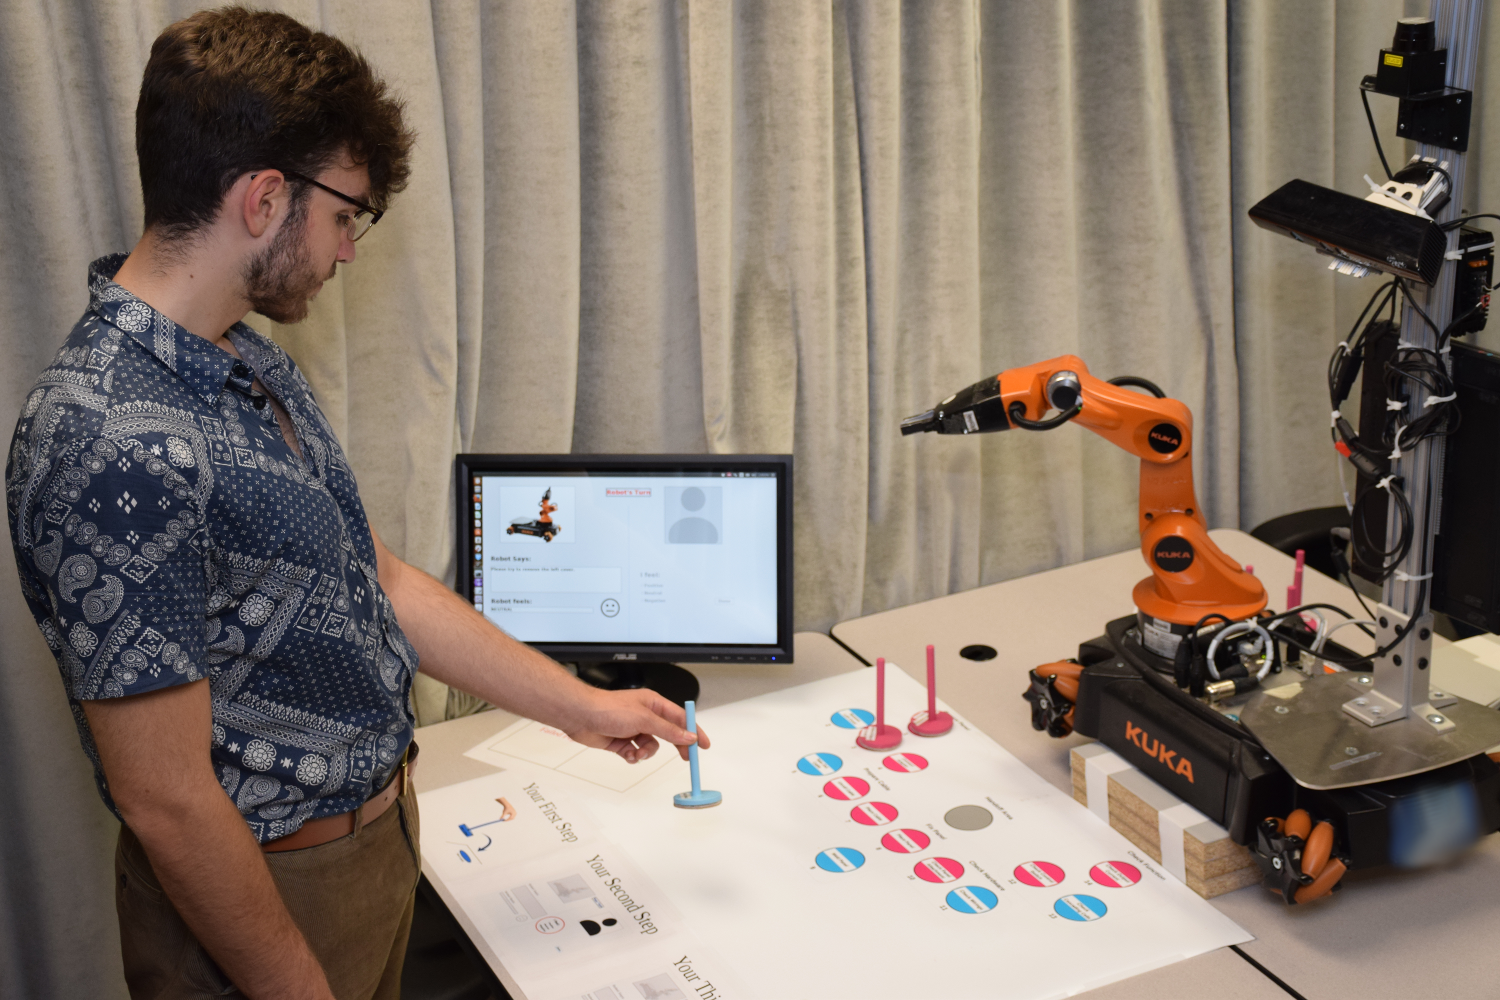
\includegraphics[scale=1.17]{figure/collaborative-robot.png}
    \caption{A robotic arm collaborating with a human to achieve a shared goal
    using \textit{Affective Motivational Collaboration} framework.}
    \label{fig:collaborative-robot}
  \end{figure*}
  
  \item \textbf{Implementing a computational system based on \textit{Affective
  Motivational Collaboration} theory:}

  In order to evaluate our computational models and algorithms within an
  interaction with human collaborators, we needed an overall functional system
  to perceive, process and act in a collaborative environment. we have
  implemented a computational system which employs our models and algorithms for
  \textit{Affective Motivational Collaboration} theory. Our computational system
  implements the key concepts related to \textit{Affective Motivational
  Collaboration} theory as well as minimal implementation of other processes
  which are required for validation of the model but are not part of this
  thesis' contributions. The emphasis of the implementation is on the underlying
  cognitive processes of collaboration and appraisal, however the implementation
  also includes the Perception and the Action mechanisms.

  \item \textbf{Validating \textit{Affective Motivational Collaboration
  Theory:}}

  (Chapter \ref{ch:awareness}) We have conducted two user studies a) to validate
  our appraisal algorithms before further development of our framework, and b)
  to investigate the overall functionality of our framework within an end-to-end
  system evaluation with participants and a robot (see Figure
  \ref{fig:collaborative-robot}). The second user study was also conducted to
  evaluate the benefit of using our computational framework in human-robot
  collaboration. In the first user study, we crowd-sourced questionnaires to
  test our hypothesis that our algorithms will provide answers similar to
  humans' to questions related to different factors within our appraisal
  algorithms. In the second user study, we investigated the importance of
  emotional awareness in human-robot collaboration, and the overall
  functionality of the AMC framework with the participants in our study
  environment.
\end{enumerate}

\chapter{Background and Related Work}
\label{ch:background}

\vspace*{-5mm}
\section{Introduction}
\vspace*{-3mm}
In this chapter, we start by reviewing the background of prominent collaboration
theories including the the SharedPlans theory \cite{grosz:plans-discourse} as
one of the two theoretical foundations of our work. We discuss the similarities
and differences between these theories (see Section
\ref{sec:collaboration-theories-comparison}) as well as related theoretical and
practical work and applications. We continue by discussing the concept of
affective computing and the social and communicative aspects of emotions from a
psychological point of view. Understanding the social aspects of emotions is
important in our work, since our work is focused on collaboration which is a
social phenomenon in human environments. We also present the concept of
artificial emotions and provide some examples of the existing computational
models of emotions. Then, we provide the background of the cognitive appraisal
theory of emotions as the second theoretical foundation in our work as well as
other computational models of emotions and the related concepts such as some
examples of cognitive architectures and the influence of affect in
decision-making procedures. This chapter continues with a description of motives
and related theories in psychology and artificial intelligence. The role of
motives as goal-driven affective components is crucial in our work, since the
collaboration structure is based on the concept of a shared goal between
collaborators. Finally, a brief description and the related work on theory of
mind in psychology and artificial intelligence is provided as another concept
used in a limited scale in our work.

\section{Computational Theories of Collaboration}
The construction of computer systems and robots that are intelligent,
collaborative problem-solving partners is important in Artificial Intelligence
(AI) and its applications. It has always been important to make computer systems
better at helping humans do whatever these systems are designed for. To build
collaborative systems, we need to identify the capabilities that must be added
to individual agents so that they can work with humans or other agents. As Grosz
says, collaboration must be designed into systems from the start; it cannot be
patched on later \cite{grosz:collaborative-systems}.

Collaboration is a special type of coordinated activity in which the
participants work jointly, together performing a task or carrying out the
activities needed to satisfy a shared goal \cite{grosz:collaboration}.
Collaboration involves several key properties at both the structural and
functional levels: most collaborative situations involve participants who have
different beliefs and capabilities; most of the time, collaborators only have
partial knowledge of the process of accomplishing the collaborative activities;
collaborative plans are more than the sum of individual plans; collaborators are
required to maintain mutual beliefs about their shared goal throughout the
collaboration; they need to be able to communicate with others effectively; they
need to commit to the group activities and to their role in it; collaborators
need to commit to the success of others; they need to reconcile between
commitments to the existing collaboration and their other activities; and they
need to interpret others' actions and utterances in the collaboration context
\cite{grosz:mice-menus}. These collaboration properties are captured by existing
computational theories of collaboration.

As mentioned above, to be collaborative, partners, e.g., a robot and a human,
need to meet the specifications stipulated by collaboration theories. These
theories argue for an essential distinction between a collaboration and a simple
interaction or even a coordination \cite{grosz:shared-plans,
lochbaum:collaborative-planning}. This section briefly provides descriptions of
major computational collaboration theories, their similarities and differences,
and their application in AI and robotics. It primarily focuses on Joint
Intention, SharedPlans and hybrid theories of collaboration. In this section, we
do not present the theories in formal language, but rather describe their
features in general terms.

The prominent collaboration theories are mostly based on plans and joint
intentions \cite{cohen:teamwork} \cite{grosz:plans-discourse}
\cite{Litman:discourse-commonsense}, and were strongly influenced by the BDI
paradigm introduced by Bratman \cite{bratman:intentions-plans} which is
fundamentally reliant on folk psychology \cite{ravenscroft:folk}. The two
theories, Joint Intentions \cite{cohen:teamwork} and SharedPlans
\cite{grosz:plans-discourse}, have been used extensively to analyze and
implement teamwork and collaboration.

The SharedPlans theory grew out of the theories of Bratman and Pollack
\cite{bratman:plans-reasoning,pollack:plan-inference,
pollack:plan-mental-attitudes}, who outlined a mental-state view of plans in
which having a plan is not just knowing how to do an action, but also having the
intention to do the actions. Bratman's views of intention goes back to the
philosophical views of Anscombe \cite{anscombe:intention} and
Casta$\tilde{n}$eda \cite{castaneda:thinking} about intention. Also, as Grosz
and Sidner mention in \cite{grosz:plans-discourse} the natural segmentation of
discourse reflects intentional behaviors in each segment.

% These intentions are designated as Discourse Segment Purposes (DSPs) which are
% the basic reasons for engaging in different segments of discourse. DSPs are a
% natural extension of Gricean intentions at the utterance level
% \cite{neale:grice-language}.

Cohen and Levesque also mention that in Joint Intentions theory their view of
intention is primarily future-directed \cite{cohen:intention-commitment} which
makes their view similar to Bratman's theory of intention
\cite{bratman:intention}, and contrary to Searle \cite{searle:collective}.\\

\textbf{Commitment} -- One of the most important concepts in teamwork and
collaboration is commitment. Collaboration theories are required to meet the
notion of commitment, otherwise the participants are just doing some coordinated
activities. Since the prominent computational collaboration theories, reviewed
in this paper, are based on Bratman's view of intention, we briefly provide his
view of commitment here before describing these theories. Bratman defines
certain prerequisites for an activity to be considered shared and cooperative
\cite{bratman:shared-activity}. He stresses the importance of:

\begin{enumerate}[a)]
  \item \textbf{Mutual commitment to joint activity} -- which can be achieved by
  agreement on the joint activity, and prevention of abandoning the activity
  without involving teammates;
  \item \textbf{Mutual support} -- which can be achieved by team members
  if they actively try to help teammate activity;
  \item \textbf{Mutual responsiveness} -- which means team members should take
  over tasks from teammates if necessary.
\end{enumerate}

In the following sections, we will see how each collaboration theory addresses
the notion of commitment.

\subsection{SharedPlans Theory}
\label{sec:sharedplans}

The SharedPlans theory of collaborative action, developed by Grosz and Sidner
\cite{grosz:planning-acting, grosz:collaboration, grosz:plans-discourse}, aims
to provide the theoretical foundations needed for building collaborative
robots or agents \cite{grosz:collaborative-systems}. SharedPlans is a general
theory of collaborative planning that requires no notion of joint intentions
(see Section \ref{sec:joint-intentions}), accommodates multi-level action
decomposition hierarchies and allows the process of expanding and elaborating
partial plans into full plans. SharedPlans theory explains how a group of agents
can incrementally form and execute a shared plan which then guides and
coordinates their activity towards the accomplishment of a shared goal.
SharedPlans is rooted in the observation that collaborative plans are not simply
a collection of individual plans, but rather a tight interleaving of mutual
beliefs\footnote{\color{red}In our framework we also have the notion of
\textit{private} beliefs (vs.\,\textit{shared} beliefs) which the other
collaborator does not know about these beliefs.} and intentions of different
team members. In \cite{grosz:collaboration} Grosz and Kraus use first-order
logic to formalize SharedPlans.

Grosz and Sidner in \cite{grosz:plans-discourse} present a model of plans to
account for how agents with partial knowledge collaborate in the construction of
a domain plan. They are interested in the type of plans that underlie discourse
in which the agents are collaborating in order to achieve a shared goal. They
propose that agents are building a shared plan in which participants have a
collection of beliefs and intentions about the actions in the plan. Agents have
a library of how to do their actions, i.e. recipes. These recipes may partially
specify how an action is executed, or contributes to a goal. Then, each agent
communicates its beliefs and intentions by making utterances about what actions
they can contribute to the shared plan. This communication leads to the
construction of a shared plan, and ultimately termination of the collaboration
with each agent mutually believing that there exists one agent who is going to
execute an action in the plan, and the fact that that agent has intention to
perform the action, and that each action in the plan contributes to the goal
\cite{grosz:plans-discourse} \cite{lochbaum:plan-models}.

Later, we will see that to successfully complete a plan the collaborators must
mutually believe that they have a common goal and have agreed on a sequence of
actions for achieving that goal. They should believe that they are both capable
of performing their own actions and intend to perform those actions while they
are committed to the success of their plans.

\subsubsection{Recipes}
\label{sec:recipe}

The SharedPlans theory differentiates between knowing how to accomplish a goal
(a recipe) and having a plan, which includes intentions. The SharedPlans
definition of mutual beliefs states that when agents have a shared plan for
doing some action, they must hold mutual beliefs about the way in which they
should perform that action \cite{grosz:collaboration,grosz:plans-discourse}.
Following Pollack \cite{pollack:plan-mental-attitudes}, the term recipe refers
to what collaborators know when they know a way of doing an action. Recipes are
specified at a particular level of detail. Although the agents need to have
mutual beliefs about actions specified in the recipe, they do not need to have
mutual beliefs about all levels of performing actions. Therefore, having mutual
beliefs of the recipe means that the collaborators hold the same beliefs
about the way in which an action should be accomplished. Consequently, the
collaborators need to agree on how to execute an action. Recipes are
aggregations of action-types and relations among them. Action-types, rather than
actions, are the main elements in recipes. Grosz and Sidner in their earlier
work \cite{grosz:plans-discourse} have considered only simple recipes in which
each recipe consisted of only a single action-type relation
\cite{lochbaum:plan-models}. Recipes can be partial, meaning they can expand and
be modified over time.

Grosz and Sidner propose that collaboration must have the following three
elements, which also indicates the importance of the shared plan:

\begin{enumerate}
  \item the participants must have commitment to the shared activity;
  \item there must be a process for reaching an agreement on a recipe for the
  group action;
  \item there must be commitment to the constituent actions. 
\end{enumerate}

\textit{Shared plan} is an essential concept in the collaboration context.
The definition of the shared plan is derived from the definition of plans
Pollack introduced in \cite{pollack:plan-inference,
pollack:plan-mental-attitudes} since it rests on a detailed treatment of the
relations among actions and it distinguishes the intentions and beliefs of an
agent about those actions. However, since Pollack's plan model is just a simple
plan of a single agent, Grosz and Sidner extended that to plans of two or more
collaborative agents. The concept of the shared plan provides a framework in
which to further evaluate and explore the roles that particular beliefs and
intentions play in collaborative activity \cite{lochbaum:plan-models}. However,
Pollack's formulation of shared plans (a) could only deal with activities that
directly decomposed into single-agent actions, (b) did not address the
requirement for the commitment of the agents to their joint activities, and (c)
did not adequately deal with agents having partial recipes
\cite{grosz:collaboration}. Grosz and Kraus in \cite{grosz:collaboration},
reformulate Pollack's definition of the individual plans
\cite{pollack:plan-mental-attitudes}, and also revise and expand the SharedPlans
to address these shortcomings.

Figure \ref{fig:plans} shows what we need to add to individual plans in order to
have plans for group actions. The top of the figure lists the main components
for individual plans. First, an individual agent needs to know the recipe for an
action, whereas agents in a group need to have a mutual belief of a recipe for
an action (bottom of the figure). In the case of a group plan, having a mutual
belief of a recipe, leads the agents to agree on how they are going to execute
the action. Then, similar to individual agents that need to have the ability to
perform the constituent actions in an individual plan and must have intentions
to perform them, the participants in a group activity need to have individual or
group plans for each of the constituent actions in the mutually agreed recipe
\cite{grosz:collaborative-systems, grosz:plans-discourse}.

\begin{figure}[tbh]
  \center
  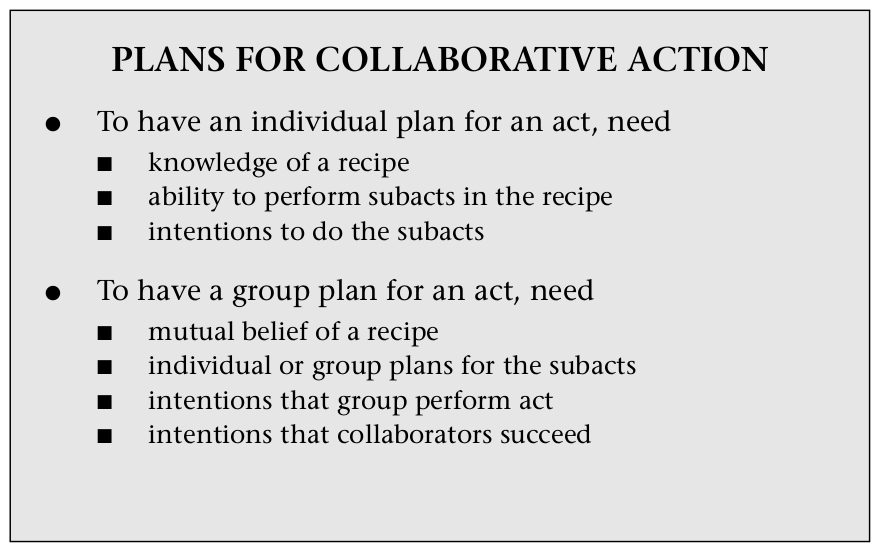
\includegraphics[width=0.8\textwidth]{figure/plans.png}
  \caption{Plans for collaborative action \cite{grosz:collaborative-systems}.}
  \label{fig:plans}
\end{figure}

As shown in Figure \ref{fig:plans} (bottom), plans for group actions include two
essential constituents that do not have correlates in the individual plan.
First, the agents need to have a commitment to the group activity; All the
agents need to intend that the group will do the action. {\color{red}{For
instance, when a robot and an astronaut are collaborating to install a solar
panel, they need to have intentions to install the solar panel together.}} Among
other things, these intentions will keep them both working on the panels until
the panels are installed. Second, the participants need to have some commitment
to the other agents to succeed in their own their actions. For instance, the
robot must have an intention that the astronaut be able to measure the quality
of installation successfully. This intention will prevent the robot from
interrupting the astronaut's measurement action or prevent the robot from using
the astronaut's measurement tool \cite{grosz:collaborative-systems,
grosz:plans-discourse}.

\subsubsection{Full Vs. Partial Shared Plan}
\label{sec:full-partial-plan}

The SharedPlans formalization distinguishes complete (full) plans and partial
plans. A shared plan can be either a \textit{Full Shared Plan (FSP)} or a
\textit{Partial Shared Plan (PSP)}. An \textit{FSP} is a complete plan in which
agents have fully determined how they will achieve a shared goal. A \textit{PSP}
definition provides a specification of the minimal mental state requirements for
collaboration to exist and gives criteria governing the process of completing
the plan.

An \textit{FSP} to do $\alpha$ represents a situation where every aspect of a
joint activity $\alpha$ is fully determined. This includes mutual belief and
agreement in the complete recipe to do $\alpha$. A recipe is a specification of
a set of actions \textit{$A_i$}, which constitutes the performance of $\alpha$
when executed under specified constraints. \textit{FSP(\textbf{P}, $\Theta,
\alpha, T_p, T_\alpha, \textbf{R}_\alpha$)} denotes a group $\Theta$'s plan
\textit{\textbf{P}} at time \textit{$T_p$} to do action $\alpha$ at time
\textit{$T_\alpha$} using recipe \textit{$\textbf{R}_\alpha$}. In short,
\textit{FSP} holds if and only if the following conditions are satisfied:

\begin{enumerate}
  \item All members of group $\Theta$ mutually believe that they intend to do
  $\alpha$.
  \item All members of group $\Theta$ mutually believe that
  \textit{$\textbf{R}_\alpha$} is the recipe for $\alpha$.
  \item For each step \textit{$A_i$} in recipe \textit{$\textbf{R}_\alpha$}:
  \begin{itemize}
    \item A subgroup $\Theta_j$ has an \textit{FSP} for \textit{$A_i$}, using
    recipe \textit{${\textbf{R}_A}_i$}.
    \item Other members of group $\Theta$ believe that there exists a recipe
    such that subgroup $\Theta_j$ can bring about \textit{$A_i$} and have an FSP
    for \textit{$A_i$}.
    \item Other members of group $\Theta$ intend that subgroup $\Theta_j$ can
    bring about \textit{$A_i$} using some recipe.
  \end{itemize}
\end{enumerate}

Most times a team and its members do not possess an \textit{FSP} to achieve
their shared goal. SharedPlans uses the concept of \textit{PSP} as a snapshot of
the team's mental states in different situations, which further leads to
communication and planning to fulfill the conditions of an \textit{FSP}. The
idea behind \textit{PSP} is enabling the agents to modify the shared plan over
the course of planning without impairing the achievement of the shared goals.
Notice that for the same reason recipes also can be partial
\cite{grosz:collaboration, grosz:plans-discourse}.

\subsubsection{Communicating Intentions}
In SharedPlans, Grosz and Sidner are interested in the type of plans that
underlie a discourse in which the agents collaborate to achieve a shared goal.
Here we briefly present their view of discourse structure, since it is related
to the intentions behind collaborators' actions. In
\cite{grosz:plans-discourse}, Grosz and Sidner argue that the SharedPlans theory
recognises three interrelated levels of discourse structure, and the components
of the discourse structure are a trichotomy of linguistic structure, intentions
structure and the attention state. In their work, the linguistic structure of a
discourse is a sequence of utterances aggregating into discourse segments just
as the words in a single sentence form constituent phrases. They also discuss
the idea of the discourse purpose as the intention that underlies engagement in
the particular discourse. They believe this intention is the reason behind
performing a discourse rather than some other actions, and also the reason
behind conveying a particular content of the discourse rather than some other
contents.
%They describe mechanisms for plan analysis looking at Discourse
%Segment Purposes (DSPs). In fact, the DSPs specify how the discourse segments
%contribute to achieving the overall discourse purpose. 
Finally, the third component in their theory, the attentional state, provides an
abstraction of the agent's focus of attention as the discourse unfolds. 
%The focusing structure contains DSPs and the stacking of focus spaces reflects
%the relative salience of the entities in each space during the discourse. 
In short, the focusing structure is the central repository for the contextual
content required for processing utterances during the discourse
\cite{grosz:plans-discourse}. 
%Using discourse plans can help to encode the knowledge about conversation.

\subsubsection{Intention-to and Intention-that}
\label{sec:intend-to-that}

In Grosz and Sidner's SharedPlans theory \cite{grosz:plans-discourse}, two
intentional attitudes are employed: \textit{intending to} (do an action) and
\textit{intending that} (a proposition will hold). The notion of
\textit{intention to}, as an individual-oriented intention, models the intention
of an agent to do any single-agent action while the agent not only believes that
it is able to execute that action, but it also commits to doing so. In short,
it is an intention to perform an action, similar to Bratman's view of intention.
In contrast with \textit{intention to}, an \textit{intention that}, as an
intention directed toward group activity, does not directly imply an action. In
fact, an individual agent's \textit{intention that} is directed towards its
collaborators' action or towards a group's joint action. \textit{Intention that}
guides an agent to take actions (including communication), that enable or
facilitate other collaborators to perform assigned tasks. This leads an agent to
behave collaboratively. Therefore, agents will adopt intentions to communicate
about the plan \cite{grosz:collaboration}. As another difference,
\textit{Intention to} commits an agent to means-end reasoning and acting
\cite{bratman:intentions-plans} while \textit{Intention that} does not
necessarily entail this commitment. The key point about \textit{Intention to}
and \textit{intention that} is that both commit an agent not to adopt
conflicting intentions, and constrain replanning in case of failure. Further, an
agent can \textit{intention that} another agent achieve the specified
proposition.

\subsection{Joint Intentions Theory}
\label{sec:joint-intentions}

Also starting with Bratman's guidelines, Cohen and Levesque propose a different
and more formal approach to building artificial collaborative agents. The Joint
Intentions theory of Cohen and Levesque \cite{cohen:teamwork,
cohen:intention-commitment, cohen:persistence-intention-commitment,
cohen:intentions, levesque:acting-together} represents one of the first attempts
to establish a theory of collaboration expressed in formal logic, and due to its
clarity, is a widely used teamwork theory.

A joint intention is a shared commitment to perform an action while in a group
mental state \cite{cohen:intention-commitment}. Joint Intentions theory is based
on individual and joint intentions (as well as commitments) to act as a team
member. A joint intention is viewed not only as a persistent commitment of the
team to a shared goal, but also implies a commitment on the part of all its
members to a mutual belief about the state of the goal. In other words, Joint
Intentions theory describes how a team of agents can jointly act together by
sharing mental states about their actions while an intention is viewed as a
commitment to perform an action.

In \cite{cohen:teamwork} Cohen and Levesque establish that a joint intention
cannot be defined simply as individual intention with the team regarded as an
individual. The reason is that after the initial formation of an intention, team
members may diverge in their beliefs and their attitudes towards the intention.
Instead, they first present a definition of individual persistent goal and
individual intention. Then, they define team analogues of these concepts by
presenting mutual belief in place of individual belief. The definition of joint
persistent goal requires each team member to commit to informing other members,
if it comes to believe that the shared goal is in its terminal status. As a
result, in Cohen and Levesque's theory, a team with a joint intention is a group
that shares a common objective and a certain shared mental state
\cite{jarvis:teams-multiagent-systems}.

In this theory, once an agent entered into a joint commitment with other agents,
the agent should communicate its private beliefs with other team members if the
agent believes that the joint goal is in its terminal status, i.e., either the
joint goal is achieved, or it is unachievable, or irrelevant
\cite{wilsker:study-theories}. Thus, as we mentioned above, team members are
committed to inform other team members when they reach the conclusion that a
goal is achievable, impossible or irrelevant. For instance, if a robot and an
astronaut are collaborating to install a solar panel, and the robot reaches the
conclusion that the welding tool has a deficiency, it is essential for the robot
to have an intention to communicate with the astronaut and make this knowledge
common. Therefore, according to this theory, in a collaboration, agents can
count on the commitment of other members, first to the goal and then to the
mutual belief of the status of the goal.

\subsubsection{Individual Commitment}
\label{sec:individual-commitment}

As we mentioned earlier, intentions and commitments are the basic ideas of Joint
Intentions theory. Here, we provide the definition of ``individual commitment''
(also called \textit{persistent goal}) by Cohen et.\,al. in
\cite{cohen:team-formation}. According to their definition an agent has a
persistent goal relative to q to achieve p only when:

\begin{enumerate}
  \item agent believes that p is currently false;
  \item agent wants p to be true;
  \item it is true (and agent knows it) that (2) will continue to hold until the
  agent comes to believe either that p is true, or that it will never be true,
  or that q is false.
\end{enumerate}

Note that the condition q is an ``escape'' clause, which can be omitted for
brevity, or it can be used as a reason for the agent to drop a commitment, even
though it could be quite vague.

\subsubsection{Individual Intention}
\label{sec:individual-intention}

As we mentioned above, Joint Intention theory adopts Bratman's view of
future-directed properties of intention. In this theory, an intention is defined
to be a commitment to act in a certain mental state. In other words, an agent
intends relative to some condition to do an action when it has a persistent goal
or commitment (relative to that condition) of having done the action and,
moreover, believing throughout that it is doing that action
\cite{cohen:teamwork}.

Intention inherits all the properties of commitment (e.g., consistency with
mental states). Typically, an agent uses an intention as a decision within a
goal hierarchy to do a particular action. For instance, initially, the agent
commits to p becoming true without having any concern about who or how p is
going to be accomplished. Then, the agent commits to x or y as a mean to
accomplish p. Lastly, the agent selects one of the actions (e.g., x) and forms
an intention to do it. This intention will be given up when for whatever reason
p is accomplished.

% \subsubsection{Joint Commitment}
% \label{sec:jpg}
% 
% Before discussing joint commitment, we provide the definition of the
% \textit{Weak Achievement Goal} (WAG) concept in Joint Intentions theory which
% shows the state of a team member nominally working on a goal. The concept of WAG
% is used to provide the definition of the Joint Commitment in this theory.\\

An agent has a WAG relative to q and with respect to a team to bring about p if
either of the following conditions holds:

\begin{itemize}
  \item The agent has a normal achievement goal to bring about p; that is, the
  agent does not yet believe that p is true and wants p to be true as a goal.
  \item The agent believes that p is true, will never be true, or is irrelevant,
  but has as a goal that the status of p be mutually believed by all the team
  members.
\end{itemize}

% \textbf{Joint commitment} -- A joint intention of a team $\Theta$ is based on
% its joint commitment, which is defined as a \textit{Joint Persistent Goal}
% (JPG). A JPG to achieve a team action p, denoted JPG($\Theta$, p) requires all
% team members to mutually believe that p is currently false and want p to
% eventually be true. A JPG guarantees that team members cannot decommit until p
% is mutually known to be \textit{achieved, unachievable} or \textit{irrelevant}.
% Basically, JPG($\Theta$, p) requires team members to each hold p as a
% \textit{Weak Achievement Goal} (WAG), where WAG($\mu$, p, $\Theta$) in which
% $\mu$ is a team member in $\Theta$, requires $\mu$ to achieve p if it is false.
% However, if $\mu$ privately believes that p is either achieved, unachievable or
% irrelevant, JPG($\Theta$, p) is dissolved, but p is left with a commitment to
% have this belief become $\Theta$'s mutual belief. Such a commitment is required
% to establish mutual belief in $\Theta$; this commitment typically makes an agent
% communicate with its teammates \cite{cohen:teamwork}.
% 
% An important consequence of achieving joint commitment in a team is that it
% predicts future communication which is critical within the course of a
% collaboration. Thus, this communication leads team members to attain mutual
% beliefs which is a fundamental concept in teamwork activities. Notice that
% the minimum mutual belief for team members to attain is the achievement or
% failure of the shared goal which terminates collaboration.

\subsubsection{Joint Commitment and Joint Intention}
A joint intention of a team is based on its joint commitment, which is defined
as a \textit{Joint Persistent Goal} (JPG)\footnote{\color{red}Castelfranchi in
\cite{castelfranchi:commitments-aids} criticizes the necessary and sufficient
conditions for the joint persistent goal. He argues that these conditions are
not sufficient for the collaborators working as a team.}. A JPG to achieve a
team action p, requires all team members to mutually believe that p is currently
false and want p to eventually be true. A JPG guarantees that team members
cannot decommit until p is mutually known to be \textit{achieved, unachievable}
or \textit{irrelevant}. This commitment typically makes an agent communicate
with its teammates \cite{cohen:teamwork}.

Therefore, an important consequence of achieving joint commitment in a team is
that it predicts future communication which is critical within the course of a
collaboration. Thus, this communication leads team members to attain mutual
beliefs which is a fundamental concept in teamwork activities. Notice that
the minimum mutual belief for team members to attain is the achievement or
failure of the shared goal which terminates collaboration.

Joint intention is defined to be a joint commitment to the team members trying
to do a joint action. Based on Cohen and Levesque's definition of joint
intention, a team of agents jointly intends (relative to some escape condition)
to do an action if and only if the members have a JPG (relative to that
condition) of them having the action completed, and having it completed
mutually believing throughout that they are doing it (knowingly)
\cite{cohen:teamwork}.

\subsubsection{Teamwork \& Communication}

In summary, according to Joint Intentions theory, the notion of teamwork is
characterized by joint commitment, also known as joint persistent goal (JPG).
The definition of JPG states that the agents mutually believe they have the
appropriate goal, and that they mutually believe a persistent weak achievement
goal (which represents the one-way commitment of one agent directed towards
another) to achieve it persists until the agents mutually believe that the goal
has either been achieved, or become impossible or irrelevant. 

Joint Intentions theory claims that an efficient collaboration requires
communication. Sharing information through communication is critical given that
collaborators have different capabilities, and each individual often has only
partial knowledge relevant to solving the problem, and sometimes diverging
beliefs about the state of the collaborative activity. Communication is
important in coordinating team members' roles and actions to accomplish their
goal. For instance, it can help team members to establish and maintain a set of
mutual beliefs regarding the current state of the collaboration, and the
respective roles and capabilities of each member.

\subsection{STEAM -- A Hybrid Approach}

Tambe in \cite{tambe:flexible-teamwork} argues that teamwork in complex,
dynamic, multi-agent domains requires the agents to obtain flexibility and
reusability by using integrated capabilities. Tambe created STEAM
(\textbf{S}hell \textbf{TEAM}work) based on this idea. STEAM's
operationalization in complex, real-world domains is the key in its success in
addressing important teamwork issues, some of which are discussed in Section
\ref{sec:applicaiton}. STEAM is founded on the Joint Intentions theory and it
uses joint intentions as the basic building block of teamwork but is also
informed by key concepts from SharedPlans theory.

Building on the well developed theories of Joint Intentions and SharedPlans, the
STEAM teamwork model was operationalized as a set of domain-independent rules
that describe how teams should work together. According to Tambe, there are
several advantages due to his use of Joint Intentions theory, including
achieving a principled framework for reasoning about coordination and
communication in a team. Another advantage is guidance for monitoring and
maintenance of a team activity which the joint commitment concept in joint
intention provides. And lastly, Tambe believes the joint intention in a team can
facilitate reasoning about team activity and team members' contribution to that
activity.

However, he also believes that for a high level team goal, one single joint
intention is not sufficient to achieve all these advantages. STEAM therefore
borrows some of the concepts of SharedPlans theory. First, STEAM uses the
concept of ``intention that'' (see Section \ref{sec:sharedplans}) towards an
activity as well as the fact that SharedPlans theory mandates team members'
mutual belief in a common recipe and shared plans for individual steps in the
common recipe. Thus, in this case, SharedPlans helps STEAM to achieve coherency
within the teamwork. In addition, STEAM uses joint intentions to ensure the
teamwork coherency to build the mental attitudes of team members. In other
words, as the recipe evolves, STEAM requires all team members to agree on the
execution of a step and form joint intentions to execute it while other joint
intentions are formed, leading to a hierarchy. A second concept STEAM borrows
from SharedPlans is the amount of information that a team member needs to know
to perform an action. According to SharedPlans, team members require to know
only that a recipe exists to enable them to perform actions (not the recipe
details -- see Section \ref{sec:recipe}). Similarly in STEAM, team members only
track the subteam or individual team member responsible to perform a specific
step; this tracking does not need detailed plan recognition. The third concept
is parallel to what is called an unreconciled case in SharedPlans theory, which
in STEAM is handled by replanning and communication between team members
assigning the unassigned or unachieved task. The last concept is communication
between team members which also borrows the concept of ``intention that'' from
SharedPlans theory, to help the generalization of STEAM's communication
capabilities beyond what Joint Intentions theory offers.

In summary, STEAM builds on both Joint Intentions theory and SharedPlans theory
and tries to overcome their shortcomings. Based on Joint Intentions, STEAM
builds up hierarchical structures that parallel the SharedPlans theory. Hence,
STEAM formalizes commitments by building and maintaining Joint Intentions, and
uses SharedPlans to formulate the team's attitudes in complex tasks.

In \cite{tambe:flexible-teamwork} Tambe argues that the novel aspects of STEAM
relate to its teamwork capabilities. A key novelty in STEAM is team operators.
In STEAM, when agents select a team operator for execution, they instantiate a
team's joint intentions. Team operators explicitly express a team's joint
activities, unlike the individual operators which express an agent's own
activities. Hence, STEAM agents maintain their own private (to apply individual
operators) and team states, e.g., mutual belief about the world (to apply team
operators).

Tambe added further practical concepts into STEAM's architecture. For instance,
STEAM has a team synchronization protocol to establish joint intention, and it
has constructs for monitoring joint intentions which helps the agent to monitor
team performance. STEAM facilitates this monitoring by exploiting its explicit
representation of team goals and plans. In particular, STEAM allows an explicit
specification of monitoring conditions to determine achievement, unachievability
or irrelevancy conditions of team operators. Finally, in STEAM, communication is
driven by commitments embodied in the Joint Intentions theory, i.e., team
members may communicate to obtain mutual belief while building and disbanding
joint intentions. Thus, joint intentions provide STEAM with a principled
framework for reasoning about communication. Also, STEAM addresses some
practical issues not addressed in other teamwork theories. One of these issues
is STEAM's detailed attention to communication overheads and risks, which can be
significant \cite{tambe:agent-archtecture-teamwork}. Furthermore,
operationalization of STEAM is based on enhancements to the Soar architecture
\cite{laird:soar}, plus a set of about 300 domain-independent Soar rules.

\subsection{Other Approaches}

There are other frameworks, approaches, and models focusing on teamwork and
collaborative agents. For instance, Jennings developed the Joint Responsibility
framework which is specified formally using modal temporal logic. Joint
Responsibility stresses the role of joint intentions (based on Joint Intentions
theory) specifying how both individuals and teams should behave whilst engaged
in collaborative problem solving \cite{jennings:joint-responsibility,
jennings:on-responsible, jennings:joint-intention-hybrid,
jennings:joint-responsibility-dynamic}. Jennings has developed Generic Rules and
Agent model Testbed Environment (GRATE) as a prototype system based on the Joint
Responsibility framework. In \cite{kinny:planned-team} Kinny et.\,al.\,elaborate
the concept of Planned Team Activity and introduce a language for representing joint plans for teams of agents and describe how agents can
organize the formation of a skilled team to achieve a joint goal. They use joint
intentions to capture the mental properties which characterize team activity.

\subsection{Similarities and Differences}
\label{sec:collaboration-theories-comparison}
There are some similarities between SharedPlans and Joint Intentions theories:

\begin{enumerate}
  \item Similar to SharedPlans theory, Joint Intentions theory specifies what it
  means for agents to execute actions as a team
  \cite{subramanian:joint-intention-dialogue}.
  
  \item Both theories follow Bratman's basic ideas about the roles of intention
  in relational actions which prevent the collaborative agents from adopting
  conflicting intentions. Both theories also follow Bratman's BDI model.
  
  \item Just as SharedPlans theory, Joint Intentions theory states that a
  joint action cannot be seen simply as a collection of individual actions, but
  rather as agents working together who need to share beliefs.
  
  \item Both theories in their mature forms emphasize that agents are required
  to communicate to maintain collaboration. SharedPlans theory requires
  collaborators to communicate to establish and maintain the shared plan, which
  is crucial especially when collaborators only have a partial shared plan.
  Similarly in Joint Intentions theory, communication is an explicit requirement
  of collaborative agents until the shared goal is achieved, unachievable or
  irrelevant.
  
  \item Both Joint Intentions and SharedPlans theories are concerned about
  commitment to the joint activity. However, these two theories use different
  concepts to fulfill the requirements of commitment during collaboration.
\end{enumerate}

There are also differences between SharedPlans and Joint Intention theories:

\begin{enumerate}
  \item The crucial components of the SharedPlans theory (see Section  
  \ref{sec:sharedplans}) lack the notion of a joint intention, which is the most
  significant notion within the Joint Intentions theory. For philosophocal
  reasons, Grosz and Sidner do not believe that such a phenomenon (joint
  intention) exists in a collaboration. They believe their notion of ``intention
  that'' and mutual beliefs about states of the collaboration can provide
  similar functionalities as described in Joint Intentions theory (see Section
  \ref{sec:joint-intentions}).
  
  \item In SharedPlans theory teammates agree on the shared plan, whereas in
  Joint Intentions theory teammates agree on intentions.
  
  \item In contrast to Joint Intentions, the SharedPlans theory employs
  hierarchical structures over intentions, thus overcoming the shortcoming of
  a single joint intention for complex team tasks.
  
  \item The SharedPlans theory describes the way to achieve a common goal
  through the hierarchy of plans, whereas the Joint Intentions theory describes
  only this common goal \cite{skubch:modelling-behavior-robots}.
  
  \item Joint Intentions theory assumes that knowledge about the teammates is
  always available, whereas SharedPlans theory uses the concept of partial
  plan/recipe to make the process of dynamically achieving information possible
  throughout the collaboration.
  
  \item Communication requirements are derived from ``intention that'' in
  SharedPlans theory, as opposed to being ``hard wired" in Joint Intentions
  theory.
\end{enumerate}

% \textbf{A critique to Joint Intention theory} -- Castelfranchi criticizes the
% necessary and sufficient conditions (see Section \ref{sec:joint-intentions}) for
% the joint persistent goal which plays a crucial role in the Joint Intentions
% theory. According to his example, if a French scientist and an American
% scientist are both working on an AIDS vaccine and both have the final goal of p
% ``vaccine anti-AIDS be found'' relative to the belief q that ``if vaccine is
% found, AIDS is wiped out'', they both share the mental attitudes described
% in Joint Intentions theory. It means that they mutually believe that p is
% currently false, and they mutually know they both want p to be true, and it is
% true that until they come to believe either that p is true, that p will never be
% true, or that q is false, they will continue to mutually believe that they each
% have a weak achievement goal (see Section \ref{sec:joint-intentions}) relative
% to q and with respect to the team (i.e., the WAG with respect to the team has
% been defined as ``a goal that the status of p be mutually  believed by all the
% team members''). The problem is that we can not claim the French and American
% professors are working as a team. In fact, given their personal goals of finding
% the vaccine, they might come to strongly compete with each other
% \cite{castelfranchi:commitments-aids}.

\subsection{Applications of Collaboration Theories}
\label{sec:applicaiton}

There is significant practical research focusing on different aspects of
collaboration based on different collaboration theories, i.e., SharedPlans,
Joint Intentions, and hybrid theories of collaboration. In this section, we
provide some examples of implemented homogeneous and heterogeneous agent/robot
and human collaborations.

Some work focuses on the concepts of robot assistants
\cite{clancey:agent-assistants-collaboration}, or teamwork and its challenges at
cognitive and behavioral levels \cite{nikolaidis:collaboration-joint-action,
scerri:prototype-distributed-teams}. Some researchers have taken an overall look
at a collaboration concept at the architectural level. In
\cite{garcia:collaboration-emotional-awareness} authors present a collaborative
architecture, COCHI, to support the concept of emotional awareness. In
\cite{esau:integrating-emotion-collaboration} authors present the integration of
emotional competence into a cognitive architecture which runs on a robot, MEXI.
In \cite{sofge:collaboration-humanoid-space} authors discuss the challenges of
integrating natural language, gesture understanding and spatial reasoning of a
collaborative humanoid robot situated in space. The importance of communication
during collaboration has also been considered by some researchers from
human-computer interaction and human-robot collaboration
\cite{clair:action-intention-collaboraiton,
matignon:verbal-nonverbal-collaboration, rich:discourse} to theories describing
collaborative negotiation, and discourse planning and structures
\cite{andriessen:disourse-planning, grosz:discourse-structure,
sidner:discourse-collaborative-negotiation}. There are other concepts such as
joint actions and commitments \cite{grosz:intention-dynamics-collaboration},
dynamics of intentions during collaboration \cite{levesque:acting-together}, and
task-based planning providing more depth in the context of collaboration
\cite{burghart:cognitive-architecture-robot, rich:cea}. The concept of
collaboration has also received attention in industries and academic robotic
laboratories \cite{green:collaboration-literature-review}.

\textbf{Applications of SharedPlans Theory} -- COLLAGEN
\cite{rich:collaboration-manager, rich:discourse} is the first implemented
general tool for collaboration based on the SharedPlans theory. It incorporates
algorithms for discourse generation and interpretation, and is able to maintain
a segmented interaction history, which facilitates the discourse between the
human user and the intelligent agent. The model includes two main parts: (1) a
representation of a discourse state and (2) a discourse interpretation algorithm
for the utterances of the user and agent
\cite{rickel:discourse-theory-dialogue}. In
\cite{heeman:model-collaboration-referring} Heeman presents a computational
model of how a conversational participant collaborates in order to make a
referring action successful. This model is based on the view of language as
goal-directed behaviour, and in his work, he refers to SharedPlans as part of
the planning and conversation literature. In \cite{lochbaum:plan-models},
Lochbaum and Sidner modify and expand the SharedPlan model of collaborative
behavior \cite{grosz:plans-discourse}. They present an algorithm for updating an
agent's beliefs about a partial shared plan and describe an initial
implementation of this algorithm in the domain of network management. Lochbaum,
in \cite{lochbaum:collaborative-planning}, provides a computational model (based
on the collaborative planning framework of SharedPlans
\cite{grosz:collaboration}) for recognizing intentional structure and utilizing
it in discourse processing. CAST (Collaborative Agents for Simulating Teamwork)
\cite{yen:cast} \cite{yin:knowledge-based-sharedplans} is a teamwork framework
based on SharedPlans theory. CAST focuses on flexibility in dynamic environments
and on proactive information exchange enabled by anticipating what information
team members will need. Petri Nets are used to represent both the team structure
and the teamwork process, i.e., the plans to be executed. Researchers in
\cite{hobbs:microsociology-relationship} discuss developing an ontology of
microsocial concepts for use in an instructional system for teaching
cross-cultural communication. They believe being acquainted with one another is
not a strong enough relationship from which to create a society. Hence, there is
a need for commitment and shared plans (as the basis of social life) to achieve
a shared goal. In this work, Grosz and Sidner's SharedPlans theory
\cite{grosz:plans-discourse} is used to explain the concept of shared plans
within the interpersonal relationships of societies in an industrial
environment. In \cite{hunsberger:auction-collaborative} Hunsberger and Grosz
discuss the idea of how rational, utility-maximizing agents should determine
commitment to a group activity when there is an opportunity to collaborate. They
call this problem the ``initial-commitment decision problem'' (ICDP) and provide
a mechanism that agents can use to solve the ICDP. They use the representation
of action, act-types and recipes in the SharedPlans theory in this work. In
\cite{zamfirescu:gdss} an integrated agent-based model for Group Decision
Support Systems is proposed and discussed. The decisional model that authors
outline in this paper is based on the SharedPlans theory. Rauenbusch and Grosz
in \cite{rauenbusch:decision-making-planning} formally define a search problem
with search operators that correspond to the team planning decisions. They
provide an algorithm for making the three types of interrelated decisions by
recasting the problem as a search problem. Their model respects the constraints
on mental states specified by the SharedPlans theory of collaboration. Babaian
et.\,al.\,in \cite{babaian:writers-assistant} describe Writer's Aid, a system
that deploys AI planning techniques to enable it to serve as an author's
collaborative assistant. While an author writes a document, Writer's Aid helps
in identifying and inserting citation keys and by autonomously finding and
caching potentially relevant papers and their associated bibliographic
information from various on-line sources. They believe the underlying concepts
of SharedPlans are relevent since in collaborative interfaces like Writer’s Aid,
the users establish shared goals with the system, and user and the system both
take initiative in satisfying them. In \cite{montreuil:planning-robot-activity}
researchers address high-level robot planning issues for an interactive
cognitive robot that acts in the presence of or in collaboration with a human
partner. They describe a Human Aware Task Planner (HATP) which is designed to
provide socially acceptable plans to achieve collaborative tasks. They use
notions of plans based on SharedPlans theory. In \cite{sidner:enagagement-robot}
Sidner and Dzikovska argue that robots, in order to participate in conversations
with humans, need to make use of the conventions of conversation and the means
to be connected to their human counterparts. They conducted an initial research
on engagement in human-human interaction and applications to stationary robots
performing hosting activities, such as tutoring and sales. They believe hosting
activities are collaborative because neither party completely determines the
goals to be undertaken nor the means of reaching the goal. To build a robot
host, they rely on an agent built using COLLAGEN which is a tool based on the
SharedPlans theory.\\

\textbf{Applications of Joint Intentions Theory} -- In \cite{kinny:planned-team}
authors introduce a language for representing joint plans for teams of agents.
They describe how agents can organize the formation of a suitably skilled team
to achieve a joint goal, and they explain how such a team can execute these
plans to generate complex, synchronized team activity. In this work, authors
adopt the underlying concepts of the Joint Intentions theory as the structure of
their collaborative agents. Breazeal et. al. in \cite{breazeal:humanoid-robots}
present an overview of their work towards building socially intelligent,
cooperative humanoid robots, such as Leonardo, that can collaborate and learn in
partnership with humans. They employ the Joint Intentions theory of
collaboration to implement the collaborative behaviors while performing a task
in collaboration with humans. In \cite{subramanian:joint-intention-dialogue}
the researchers' goal is to develop an architecture, based on the concepts of
Joint Intentions theory, that can guide an agent during collaborative teamwork.
They describe how a joint intention interpreter that is integrated with a
reasoner over beliefs and communicative acts can form the core of a dialogue
engine. Ultimately, the system engages in dialogue through the planning and
execution of communicative acts necessary to attain the collaborative task at
hand. Mutlu et. al. in \cite{mutlu:coordination-robot} discuss key mechanisms
for effective coordination toward informing the design of communication and
coordination mechanisms for robots. They present two illustrative studies that
explore how robot behavior might be designed to employ these mechanisms
(particularly joint attention and action observation) to improve measures of
task performance in human-robot collaboration. Their work uses Joint Intentions
theory to develop shared task representations and strategies for task
decomposition. The GRATE* system by Jennings
\cite{jennings:joint-intention-hybrid} is based on the Joint Intention theory.
GRATE* provides a rule-based modelling approach to cooperation using the notion
of Joint Responsibilities, which in turn is based on Join Intentions. GRATE* is
geared towards industrial settings in which both agents and the communication
between them can be considered to be reliable.\\

\textbf{Applications of Hybrid Theories} -- The domain independent teamwork
system, STEAM, has been successfully applied to a variety of domains.  From
combat air missions \cite{hill:synthetic-battlefield-aircraft} to robot soccer
\cite{kitano:robocup} to teams supporting human organizations
\cite{pynadath:teamwork-heterogeneous-agents} to rescue response
\cite{scerri:robot-agent-person}, applying the same set of STEAM rules has
resulted in successful coordination between heterogeneous agents. The successful
use of the same teamwork model in a wide variety of diverse domains provides
compelling evidence that it is the principles of team-work, rather than
exploitation of specific domain phenomena, that underlies the success of
teamwork based approaches. In \cite{marsella:robocup} authors provide their
RoboCup (robotics soccer testbed) in which their focus is on teamwork and
learning challenges. Their research investigation in RobotCup is based on ISI
Synthetic, a team of synthetic soccer-players. They also investigate the use of
STEAM as their model of teamwork which is influenced by the Joint Intentions and
SharedPlans theories. In \cite{kabil:coordination-mechanisms} researchers
propose a behavioral architecture C$^2$BDI that allows the enhancement of the
knowledge sharing using natural language communication between team members.
They define collaborative conversation protocols that provide proactive behavior
to agents for the coordination between team members. Their agent architecture
provides deliberative and conversational behaviors for collaboration, and it is
based on both the SharedPlans and Joint Intentions theories.

\section{Emotions and Affective Computing}
According to Picard \cite{picard:affective-computing}, the term affective
computing encompasses a new approach in artificial intelligence to building
computers that show human affection. Studies show that the decision making of
humans is not always logical \cite{GrossbergGutowski:affect-cognition}, and in
fact, not only is pure logic not enough to model human intelligence, but it also
shows failures when applied in artificial intelligence systems
\cite{dreyfus:artificial-critique}.

If we want robots and virtual agents to be more believable and efficient
partners for humans, we must consider the personal and social functionalities
and characteristics of emotions; this will enable our robots to coexist with
humans, who are emotional beings. To have a better understanding of applications
of affective computing, we can categorize the existing literature of
computational emotion modeling into four major categories: a) detecting and
recognizing human emotions, b) interpreting and understanding human emotions, c)
generating artificial emotions and applying the underlying processes to exploit
emotion functions, and d) expressing human-perceivable emotions during
interaction.

The major approaches to model emotions are \textit{appraisal, dimensional} and
\textit{discrete (basic)}, some of which have corresponding computational
models, e.g., EMA \cite{marsella:ema-process-model} and WASABI
\cite{becker:wasabi,becker:wasabi-description}. These models have been used in
different domains including AI and robotics. Applying these models can help
robots and virtual agents to achieve communicative, evaluative, interpretive,
and regulatory aspects of emotions in some or all of the four categories
mentioned above.

This section provides descriptions of the major computational emotion theories,
their comparison, and their applications in AI and robotics. It includes the
existing influential computational emotion theories as well as the underlying
psychological theories; {\color{red}we mainly focus on appraisal theory since it
emphasizes and explains the connection between emotion and cognition, although we also
discuss the dimensional theory, and we briefly cover other approaches, e.g.
discrete (basic) emotions.}

\subsection{Affect and Emotions}
Emotion influences not only what people do, but also the way they do it
\cite{cowie:concepts-definitions}. Aristotle in \emph{The Nicomachean Ethics}
reveals his idea about emotions. He says ``Anyone can become angry--that is
easy. But to be angry with the right person, to the right degree, at the right
time, for the right purpose, and in the right way--this is not easy
\cite{aristotle:ethics}.''

Intelligence is a set of mental abilities that enables a human to comprehend,
reason and adapt in the environment, and as a result, act effectively and
purposefully in that environment. Emotions play a crucial role in
scientists' explanation of humans' intelligent behaviors. Emotions significantly
impact the processes of action generation, execution, control, and
interpretation \cite{zhu:emotion-action} in different environments. Emotions are
conceptualized as ongoing processes rooted in dynamic social contexts, which can
shape both implicit and explicit emotional responses
\cite{parkinson:emotion-social-interaction}. An emotion is a dynamic episode
that not only involves changes in cognitive states, but also produces a sequence
of response patterns on body movements, posture, voice and face
\cite{scherer:expression-appraisal}. Emotions typically occur in response to an
event, usually a social event, real, remembered, anticipated, or imagined.
Emotions are associated with distinctive relational meanings
\cite{parkinson:holds-emotion}. These relations can be with the individual's
past experience, the individual's surrounding objects and environment, or the
other individuals with or without mutual beliefs in a dyadic or a group setting.
Emotions are evaluative and responsive patterns that serve the function of
providing appraisal about whether the ongoing event is harmful, threatening or
beneficial for the well-being of an individual \cite{zhu:emotion-action}.
Consequently, intelligence and emotional processes have an integral and a
supportive relationship, rather than an antagonistic or a conflicting one.

A better question than what emotions are, is the question of what they can
do, and how they impact human life. Emotions impact fundamental parts of
cognition including perception, memory, attention and reasoning
\cite{clore:judgement-regulation}. This impact is caused by the information
emotions carry about the environment and event values. The influence of emotions
depends on an individual's focus of attention. For instance, a positive affect
can cause a positive attitude towards an object if the individual's focus is on
the object, whereas the same positive affect can be interpreted as a positive
feedback towards one's partner during the course of a collaboration. As another
example, a positive feedback can promote certain cognitive processes, or it can
inhibit other cognitive processes according to the conditions in the environment
\cite{clore:affective-guidance}. In both cases, emotions play a regulatory role
for cognitive processes \cite{gross:emotion-generation-regulation}. Some of
these effects flow from underlying shifts in the way people perceive and think
under the influence of emotion.

\subsection{Emotion in Social Context}
\label{section-emotion-social}

In this section, we discuss the importance of studying emotions within a social
context. This perspective is important in our research because our work is
focused on collaboration as a particular social setting between individuals.
Understanding the dynamics of collaboration requires one to understand
influential underlying components.

Emotions are involved in developing social contexts. Humans are social and most
of the causations and constitutions of their emotions are social. Brian
Parkinson in \cite{parkinson:emotions-social} argues that many of the causes of
emotions are interpersonal and communicative rather than internal and reactive
phenomena. There are different social aspects of emotions influenced by various
factors such as social context and social relationship type. For instance, a
dominant-submissive social relationship can cause and contain different emotions
with different intensities compared to a reciprocal or a friendship social
relationship. As another example, an emotion can be interpreted in a certain way
when an individual is situated in an environment with other people who are
expressing a particular emotion.

As mentioned earlier, the social context is an important factor influencing
one's emotions. A dyadic interaction is one type of social setting
\cite{coan:emotion-dyadic}. Dyadic interaction tasks make it possible to examine
how individuals experience and express emotions during social interactions and
how emotions shape and are shaped by the reciprocal interactions between
individuals. In addition, eliciting and monitoring emotional processes yields
useful information about the role emotion plays in interpersonal relationships.
Compared with other emotion-eliciting events, events in a dyadic interaction can
better help us study an ongoing emotional relationship between two individuals
in addition to their internal emotional and cognitive processes. Dyadic
interaction tasks are ideal for studying a range of emotional responses because
of the fairly unstructured conversations between the individuals. Thus, dyadic
interaction tasks will generate a wide range of emotions in comparison with the
controlled emotion-eliciting events.

There are numerous ways that emotions can be social \cite{tiedens:social-life}.
There is a consensus on the fact that social events and entities surrounding the
individual play an essential role in the generation of emotion. There are
several ways in which other people elicit emotional responses in us. One is that
we feel the emotions of those around us. Also, we have emotions about actions of
those people around us. Another is we have emotions about the things that happen
to other people. Yet another is our concern about our relationship with others
that elicits emotion in us. The groups to which we belong can also elicit our
emotions. Moreover, we can feel emotion about the success and failure of our own
group or of other groups. In addition, groups or individuals may make salient
cultural concerns or societal expectations that can elicit our emotions.

Beside the fact that social context can elicit emotions in individuals, social
context provides information about what emotion should be expressed, by whom,
and in what situations. For instance, people are well aware of the
inappropriateness of expressing too much emotion to acquaintances
\cite{tiedens:social-life}. However, the social knowledge of emotion expression
is only partially delivered in an explicit fashion. There are studies on the
regulatory role of society and social relationships on emotions, showing that
people's emotions become socialized in implicit and unconscious ways. From this
perspective, social context can control and direct our attention toward certain
types of events and away from others.

Humans are emotional and social beings. Their emotions and the social context
in which they are involved have mutual impacts on each other. Humans can share
their emotions with others just as they share their thoughts, resources and
their environment. Sharing an emotion with others may alter the experience of an
event. For instance, according to the nature of the relationship between the
individuals, the expression of emotions can either restrain them from further
interactions or improve their relationship. Furthermore, individuals sharing
emotions might possess a shared understanding of their environment. Socially
shared and regulated emotions also provide social meanings to the events
happening in the environment \cite{wisecup:sociology-emotions}. For instance,
people are likely to make social inferences based on the presence or absence of
particular emotions in their social environment. Moreover, emotions can provide
a basis for judgment depending on the individual's relationships with others. In
other words, emotions can associate or disassociate an individual, therefore,
they can change or maintain the individual's social relationships
\cite{tiedens:social-life}.

Emotions can also play the role of a motivator in a social context. There is a
subset of social emotions delineated as role-taking emotions. In
\cite{shott:emotion-social-life} Shott provides two categories of
\textit{reflexive} (e.g., shame or pride) and \textit{empathic} (e.g., empathy
or pity) role-taking emotions. Reflexive emotions can motivate the individual's
self-control which depends on the anticipated reactions of others to the
individual's behaviors. For instance, guilt might lead the individual to behave
altruistically to restore a positive social stance for that individual. Empathic
(or vicarious) emotions are based on an individual mentally placing himself in
other's situation to understand how the other feels in that situation. These
emotions motivate prosocial behaviors to maintain an individual's internal
well-being \cite{thoits:socialogy-emotion}.

\subsection{Communicating Emotions}
\label{section-emotion-comm}

Humans need to communicate their emotions within a social context for different
reasons. In \cite{goffman:self-presentation} Goffman argues that human behaviors
around others are performative; i.e., they are often intended to convey
information to others. When a human's actions are visible in a social context,
they behave differently \cite{zajonc:social-facilitation}. The social life of an
individual is comprised of the individual's internal cognitive competencies and
his interactions in the society. Lazarus says, if society is a fabric, then
emotion is its color \cite{lazarus:emotion-adaptation}. Although emotions
undeniably have personal aspects, they are usually experienced in a social
context and acquire their significance in relation to this context
\cite{parkinson:emotion-social-interaction}.

There are several events that can elicit emotions in social contexts. For
instance, during the interaction the cause of an emotion can be verbal (an
utterance during conversation), nonverbal (someone's gesture), personal thoughts
(interpretation of an event), or even emotions themselves (e.g., happiness for a
partner's sense of pride). An utterance can include content and relational
meaning. The content carries the information about the topic or the subject of
the interaction, and the relational meaning reveals the meaning between the
speaker and the hearer. An emotion might seem to be elicited by the content of
the utterance, but in fact it is an individual's response to the relational
meaning \cite{planalp:communicating-emotion}. 

The interpretation of these relational meanings are handled by the appraisal of
the events. Appraisal processes (see Section \ref{sec:appraisal}) also
give us a way of viewing emotion as social \cite{hooft:sharing-emotions}. Meaning is
created by an individual's social relationships and experiences in the social
world. Individuals communicate these meanings through utterances. Utterances in
emotionally charged conversations, by their very nature, are supposed to inform
the others about something novel. Novelty is an essential component of an event
for appraisal. Conversations also possess the concept of consistency, because
utterances with consistent meaning constitute the individual's underlying
beliefs. Relevancy is another component of an event that can be assessed by
appraisal. The degree to which the individual's personal and mutual beliefs are
strong and related controls emotionally rich social contexts. In other words,
the more divergent the individual's beliefs, the more effort is required to
converge (to be understood) which leads to more emotional responses in
individuals. Human speech carries emotional information in the semantics and in
the speech prosody. The semantics or the content of what an individual says
includes obvious expression of emotion. The prosody holds more detailed
emotional information by combining non-semantic cues in spoken language (e.g.,
rhythm and intonation) \cite{luneski:emotion-aware-interaction}.

Interpretation of the events in a social context requires a baseline for the
individual's assessment process. Goals, as the pillar of collaborative
interactions, can provide this baseline for an individual. Goals are crucial in
relational meanings of the events in a social context. The facilitation,
interference and inhibition of goals are each correlated with certain type of
emotions. In most conversations during collaboration, goals can be categorized
into three different groups: goals related to accomplishing a task, goals to
reveal one's personal beliefs, and goals to regulate one's social relationships
\cite{planalp:communicating-emotion}. For instance, for task-related goals,
utterances related to accomplished tasks reveal joyful relational meaning;
utterances related to impeded tasks reveal disappointing relational meanings
which can lead to anger, and utterances related to tasks with no or little
progress reveal the frustration of the individuals. Lastly, all these emotional
responses in a social context will not only regulate or maintain individual's
actions to reveal or hinder an intention, but also can control the way that
action should be taken.

A successful and effective emotional communication necessitates ongoing
reciprocal adjustments between interactants that can happen by interpreting each
other's behaviors \cite{parkinson:emotion-social-interaction}. It not only
requires proper interpretation of the other's expressions, but also correct
assessment of the extent to which others can read an individual's expressions.
In emotional communication, individuals are constantly exchanging messages about
their mental states, and modifying each other's emotional responses as they
occur. Individuals perceive others' emotional states by processing verbal and
nonverbal messages during the interaction. Communication dynamics represent the
temporal relationship between these communicative messages. The verbal and
nonverbal messages from one participant are interpreted inside the context
including the history and the ongoing messages from the other individuals.
Interpersonal dynamics (also known as micro-dynamics in sociology) represent
this influence of relationships between individuals
\cite{louis:communication-dynamic}.

\subsection{Social Functions of Emotions}
\label{section-emotion-social-functions}

Humans are able to communicate their emotions in a social context. The social
functions of emotions are the reason behind why humans try to communicate their
emotions. Ekman in \cite{ekman:argument-emotions} asserts that the primary
function of emotions is to mobilize the organism to deal with important
interpersonal encounters. Darwin in \cite{darwin:emotion-expression} argues the
significance of social communicative functions of emotions. Emotions describe
interpersonal dynamics in a way that they can constitute individuals'
relationships \cite{parkinson:emotions-social, tiedens:social-life}. One aspect
of expressing and communicating emotion in a social context is to express one's
social motives and intentions \cite{hess:darwin-emotion}. Another aspect of
communicating emotions is to reveal the underlying mental states of an
individual \cite{parkinson:emotion-communication}. In other words, emotions
constitute two different functionalities of expressing communicative signals
associated with one's social motives and intentions as well as expressing one's
internal states and how one feels about something. In
\cite{kleef:emotion-regulate-social} Van Kleef has discussed the idea of
inferential processes with which individuals can infer information about others'
feelings, relational orientations and behavioral intentions based on their
emotional expressions. He also argues that emotional expressions can impact
social interactions by eliciting others' affective responses.

Functional accounts vary according to the kind of system being analyzed.
Thus, functional approaches to the emotions vary by level of analysis. Social
functions of emotions can be analyzed in \textit{individual, dyadic, group} and
\textit{cultural} levels. The focus of this research is on social functions in
dyadic interaction (more specifically collaboration); these functions are also
considered at the individual's level especially when interpreting the other
collaborator's behaviors. Studies in all these levels share a few assumptions:
a) individuals are social by nature and pursue solutions to survival problems in
social relationships, b) individuals apply their emotions to coordinate their
social interactions and relationships to address these survival problems, c)
emotions are processes mediating the individuals' relations to their dynamic
environment \cite{keltner:emotion-functions}. In dyadic interactions, studies
focus on how emotions impact the interactions of individuals in meaningful
relationships. In \cite{keltner:emotion-functions} Keltner and Haidt discuss
that in a dyadic setting, researchers mostly focus on communication of emotion
(e.g.\,Scherer \cite{scherer:vocal-expression}, DePaulo
\cite{depaulo:nonverbal-behavior}), properties (e.g.\,emotion contingency,
emotion synchrony) of dyadic emotions (e.g.\,Levenson \& Gottman
\cite{levenson:affective-exchange}), discourse (e.g.\,Bretherton
\cite{bretherton:emotions-functionalist}), and attachments (e.g. Hazan \& Shaver
\cite{hazan:emotion-attachment}).

\subsubsection{Examples of Social Emotions:}

There are many different types of emotions, only some of which are considered
social, since they appear and provide meaning in social context. Here, we
provide four examples of such emotions as well as their social functions to
show how social functions of emotions impact individuals and the groups they
belong to, and what causes them to be expressed by an individual.\\

\noindent \textbf{Guilt} -- The function of guilt is to positively direct our
behavior toward our group. We feel guilt when we hurt someone in our group, or
when we fail to reciprocate care or kindness. Guilt motivates us to not hurt
people in our group and to give back to others who have given to us, and in this
way we strengthen the survival prospects of both the group and ourselves.

\noindent \textbf{Shame} -- The function of shame is twofold. On the one hand,
it keeps us within the rules and norms of society by informing us when we have
done something dishonorable, disgraceful, or in some way condemned by our group.
On the other hand, it informs the other members of our group that we know that
we have dishonored ourselves. The main difference between guilt and shame is
that guilt is focused on a behavior, whereas shame is focused on ourselves.

\noindent \textbf{Embarrassment} -- Embarrassment is related to shame, but
includes some important differences. Embarrassment can only happen in public,
whereas shame can happen when we are alone. We can feel embarrassment about very
minor issues that have no moral implications, such as body odor, whereas shame
typically concerns more grave issues with moral implications.

\noindent \textbf{Pride} -- The function of pride is to reinforce when we or
another person has done or represented something the group finds excellent. In
this way, group values are reinforced and incentivized, which again helps the
group to function better and motivates us to do things the group values. There
is a negative form of pride in which our internal appraisal of our worth is
inflated compared to the opinions of others, which is more correctly called
hubris.

\subsection{Artificial Emotions}
\label{sec:artificial-emotions}
Emotions, as an integral part of rational behavior, provide adaptive values for
an artificial creature. They can control an agent's \textit{attention} to focus
on the most salient and relevant stimulus to solve the immediate problem. They
can also help an agent to \textit{monitor its own performance} so that the agent
can make alterations on goals and plans. Emotions can act as a \textit{memory
filter} allowing a better recall of the events that are congruent with current
cognitive and emotional states \cite{brave:emotion-hci}. \textit{Assisting the
reasoning process} is another role of emotions; they assist the reasoning
process by directing the cognitive information processes to the perceptual cues.
Emotions impact the transformation of the agent's \textit{decision-making
behavior} \cite{gmytrasiewicz:emotion-agent-decision} leading to a particular
type of actions in a certain type of environment \cite{zhu:emotion-action}.
Emotions can \textit{govern behavior tendencies} by providing immediate
emotional responses, e.g., avoidance of elaborate reasoning because of lack of
time or an unconcerned situation. Furthermore, emotions \textit{provide support
for social interactions} by helping the agent to understand others' behaviors as
well as making expressions of the agent's internal states more perceivable
during the interaction \cite{gadanho:learning-emotions}.

The importance of these values of emotions for designing social agents having
artificial emotions is apparent. However, the question is what problems are we
facing in designing an effective social agent? In
\cite{freitas:artificial-emotions-ready} authors discuss some of these problems
and provide references speculating on the nature, function and mechanisms of
emotions. Also, the importance of emotions and the incorporation of emotions in
intelligent systems as well as implementation of emotions in several multi-agent
systems are presented in \cite{miranda:emotions-humans-ai}. Scheutz discusses
the role of emotions in artificial intelligence and how we can determine the
utility of emotions for the design of an artificial agent
\cite{scheutz:emotion-role}. In \cite{botelho:machinery-emotions} the authors
present a definition and theory of artificial emotions viewed as a sequential
process comprising the appraisal of the agent's global state; they also show how
emotions are generated, represented and used in the Salt and Pepper architecture
for autonomous agents. From the behavior perspective, appropriately timed and
clearly expressed emotions are a central requirement for believable agents
\cite{bates:emotion-roles}.

There are several architectures modelling emotions for the purpose of enhancing
the believability and effectiveness of the agents and robots. But the question
is how do we model emotions? Hudlika in \cite{hudlicka:modeling-emotion}
deconstructs the concept of emotion modelling into: (a) fundamental categories
of processes for emotion generation and emotion effects, and (b) identification
of some of the fundamental computational tasks required to implement these
processes. These building blocks can be helpful as a guideline for the
systematic development of new computational models, or for the assessment of
existing computational models of emotions as discussed in
\cite{lin:computational-models-emotion} and \cite{marsella:computational}. There
are also logical formalizations of emotions and emotional attitudes (including
speech acts) and corresponding mental states to provide a systematic analysis
of computational models of emotions \cite{adam:logical-formalization,
grant:model-intention-formation, guiraud:emotions-formalization-speech-acts}.

From another perspective, the necessity of employing emotions in robotics and
more specifically social robots has been argued in
\cite{pfeifer:robotics-emotion} and \cite{sloman:robots-emotion}. Social
robotics and cognitive robotics have many overlapping concepts, especially when
they focus on interaction between a robot and a human. The relationship between
cognition and emotion receives more attention due to the mutual influences they
have on each other
\cite{morse:robotic-modelling-cognition,scheutz:emotional-states-behavior}. For
instance, in \cite{gadanho:learning-emotions} the authors employ emotions in the
learning procedure of a robot, and in \cite{broekens:affect-action-selection} and
\cite{scheutz:emotion-action-behavior} authors discuss the importance of
emotions in the action selection procedure of an agent or a robot, impacting
the behavior arbitration and self-adaptation mechanisms. Ultimately, employing
artificial emotions will impact the context of human-robot/computer interaction
\cite{hudlicka:affect-HRI} and how humans and robots understand each other's
emotions in a social environment
\cite{kirby:social-robots,canamero:emotion-robot-perspective}. In
\cite{rumbell:comparative-emotions-functions} the authors selected twelve
autonomous agents that incorporate an emotion mechanism into the action
selection procedure to compare. They introduced a framework based on
correlations between emotion roles performed and aspects of emotion mechanisms
used to perform those roles. Gratch and Marsella also present a method to
evaluate a computational model of emotion in \cite{gratch:evaluating} which
compares behavior of the model against human behavior.

\subsection{Cognitive Architectures}

There are several integrated cognitive architectures that try to produce all
aspects of behavior as a single system in different domains
\cite{anderson:act-r, laird:soar}. {\color{red}A survey on the comparison of
underlying philosophy and functional description of the most prominent cognitive
architectures introduces several criteria to evaluate such architectures}
\cite{chong:cognitive-architectures-survey,langley:cognitive-architectures,
thorisson:cognitive-architectures-autonomy}. The necessity of integrating these
cognitive architectures into robots has been discussed from the perspective of
developmental psychology \cite{asada:cognitive-robotics-humanoid,
d'mello:computational-functional-modeling,
kelley:cognitive-robotics-psychology}. There are also many examples emphasizing
the importance of cognitive robotics from this perspective, while some of them
also incorporate the concept of affect in their design
\cite{cai:affective-model-psi}. Some of these cognitive architectures are
biologically inspired, e.g., \textit{eBICA}
\cite{samsonovich:emotional-biologically-architecture}, or
\cite{baxter:cognitive-architecture-hri} and
\cite{ray:self-sustaining-architecture}, while some others are inspired by
psychological theories, e.g., $\MakeUppercase{ACT-R\Phi}$
\cite{dancy:actR-physiology-affect}, or
\cite{mirolli:vygotskyan-cognitive-robotics} and
\cite{dominey:shared-intention-cognition}.

\section{Computational Models of Emotions}
There are different types of computational theories of emotion such as
appraisal and dimensional theories. These theories differ in the type of
relationships between their components and whether a particular component plays
the crucial role in an individual emotion. For instance, the basic component of
an emotion can be the behavioral tendencies, the cognitive elements, or the
somatic processes. Emotion theories can also differ based on their
representationial distinctions.

\subsection{Appraisal Theory}
\label{sec:appraisal-theory}

Appraisal theories of emotion were first formulated by Arnold
\cite{arnold:emotion-personality} and Lazarus \cite{lazarus:emotion-adaptation}
and then were actively developed in the early 1980s by Ellsworth and Scherer and
their students \cite{roseman:appraisal-theory}
\cite{sander:systems-approach-appraisal} \cite{scherer:nature-function-emotion}
\cite{scherer:emotions-emergent} \cite{scherer:appraisal-processes}. In
general, the emotional experience is the experience of a particular situation
\cite{frijda:emotions}. Appraisal theory describes the cognitive process by
which an individual evaluates the situation in the environment with respect to
the individual's well-being and triggers emotions to control internal changes
and external actions. In this section, we are going to review sequential and
structural approaches incorporating the appraisal concept.

\begin{figure}[tbh]
  \center
  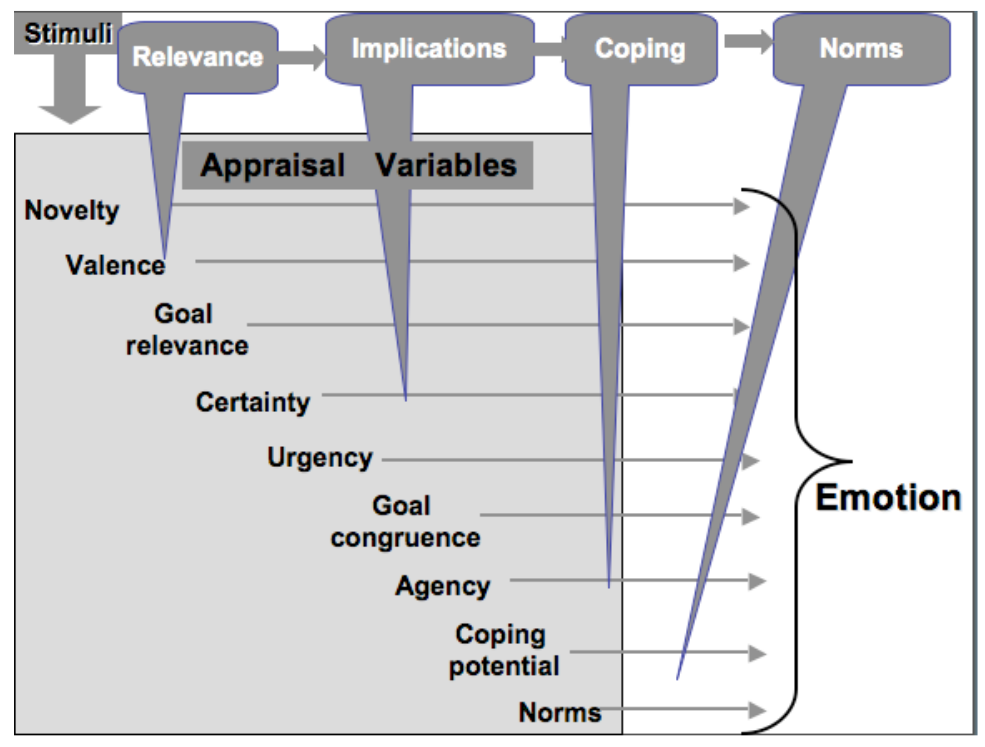
\includegraphics[width=0.8\textwidth]{figure/cpm.png}
  \caption{Schematic view of the componential theory of emotion
  \cite{hudlicka:guidelines-emotions}.}
  \label{fig:cpm}
\end{figure}

\subsubsection{Componential Approach}
\label{sec:componential-theories}

This approach emphasizes the distinct components of emotions, and is often
called the \textit{componential} approach \cite{leventhal:emotion-cognition}.
The ``components" referred to in this approach are the components of the
cognitive appraisal process. These are referred to as \textit{appraisal
variables}, and include \textit{novelty, valence, goal relevance, goal
congruence}, and \textit{coping abilities}
(later in this section some of the appraisal variables used in computational
models are introduced)
\cite{scherer:nature-function-emotion,scherer:appraisal-processes}. A stimulus,
whether real or imagined, is analyzed in terms of its meaning and consequences
for the agent, to determine the affective reaction. The analysis involves
assigning specific values to the appraisal variables. Once the appraisal
variable values are determined by the organism's evaluative processes, the
resulting vector is mapped onto a particular emotion, within the n-dimensional
space defined by the n appraisal variables. The semantic primitives for
representing emotions within this model are thus these individual appraisal
variables. Figure \ref{fig:cpm} shows the relationship of the individual
appraisal dimensions to the broader categories of evaluations taking place
during appraisal (Relevance, Implications, etc.).

\subsubsection{Component Process Model}
\label{sec:cpm}

The Component Process Model (CPM) is Scherer's influential appraisal theory of
emotions
\cite{scherer:sequential-appraisal-process,scherer:appraisal-processes}. This
theory focuses on the dynamic unfolding of emotions. The CPM suggests that an
event and its consequences are appraised with a set of criteria on multiple
levels of processing (the appraisal component). The result of the appraisal will
generally have a motivational effect, often changing or modifying the
motivational state (see Section \ref{sec:affect-motives}) before the occurrence
of the event. Based on the appraisal results and the motivational changes, some
effects will occur in the autonomic and somatic nervous system. The CPM
considers emotions as the synchronisation of many different cognitive and
physiological components. Emotions are identified with the overall process
whereby low level cognitive appraisals, in particular the processing of
relevance, trigger bodily reactions, behaviours and subjective feelings. The
model suggests that there are four major appraisal objectives required to
adaptively react to a salient event \cite{scherer:dynamic-architecture-emotion}:

\begin{enumerate}[a)]
  \item \textbf{Relevance:} How relevant is this event for the agent? Does it
  directly affect the agent or its social reference group?
  \item \textbf{Implications:} What are the implications or consequences of this
  event and how do they affect the agent's well-being and its immediate or
  long-term goals?
  \item \textbf{Coping Potential:} How well can the agent cope with or adjust to
  these consequences?
  \item \textbf{Normative Significance:} What is the significance of this event
  for the agent's self-concept and for social norms and values?
\end{enumerate}

To attain these objectives, the agent evaluates the event and its consequences
on a number of criteria or \textit{Stimulus Evaluation Checks} (SECs), with the
results reflecting the agent’s subjective assessment of consequences and
implications on a background of personal needs, goals, and values
\cite{scherer:appraisal-processes}. Figure \ref{fig:comp-cpm} shows the
postulated sequence, the cognitive and motivational inputs and the effects on
response systems. Also, the bidirectional effects between appraisal and other
cognitive functions are illustrated by the arrows in the upper part of Figure
\ref{fig:comp-cpm}.

\begin{figure}[tbh]
  \center
  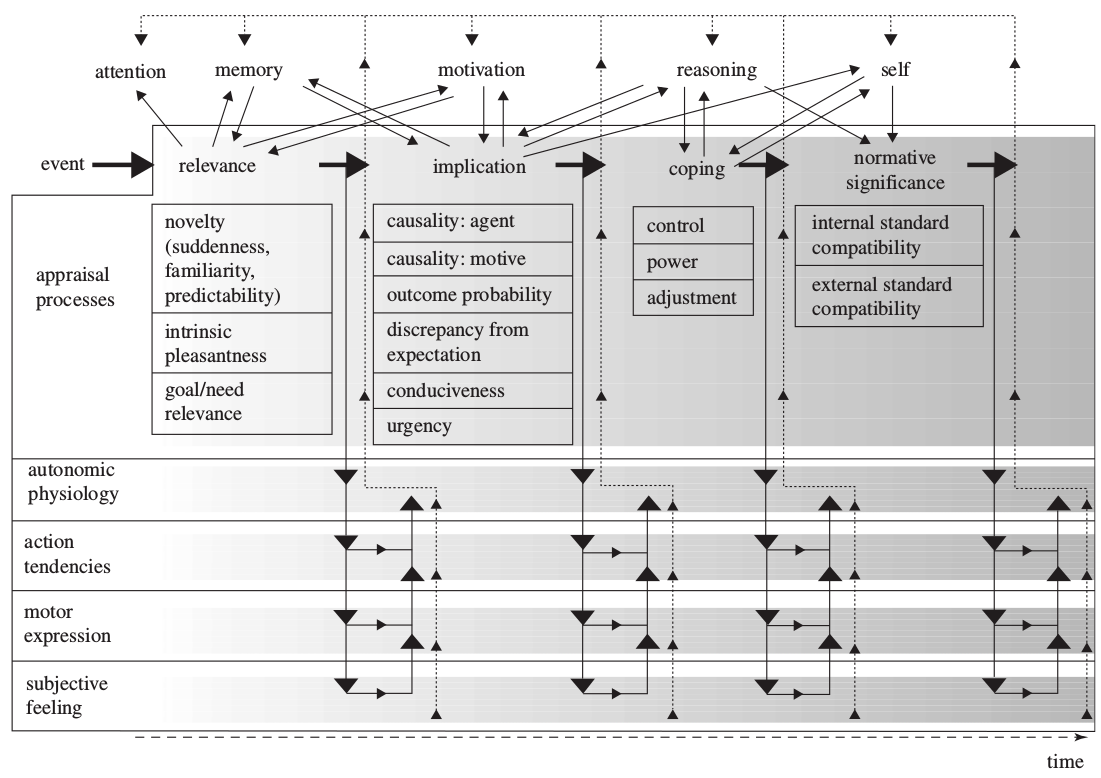
\includegraphics[width=\textwidth]{figure/comprehensive-CPM.png}
  \caption{Comprehensive illustration of the CPM of emotion
  \cite{scherer:dynamic-architecture-emotion,scherer:appraisal-processes}.}
  \label{fig:comp-cpm}
\end{figure}

\subsubsection{Appraisal Process}
\label{sec:appraisal-process}

According to appraisal theory, appraisals are separable antecedents of emotion,
that is, the individual first evaluates the environment and then feels an
appropriate emotion \cite{scherer:appraisal-processes}. The appraisal procedure
begins with the evaluation of the environment according to the internalized
goals and is based on systematic assessment of several elements
\cite{scherer:sequential-appraisal-process}. The outcome of this process
triggers the appropriate emotions. In many versions of appraisal theory,
appraisals also trigger cognitive responses often called \textit{coping
strategies}. In fact, the coping mechanism manages the individual's action with
respect to the individual's emotional state and the existing internal and/or
external demands \cite{folkman:coping-pitfalls-promise}. The majority of
computational models of emotions take this approach. An individual can also use
knowledge about the emotional reactions of others to make inferences about them.
According to the appraisal patterns, different emotions can be experienced and
expressed. Since expression of emotions reflects one's intentions through the
appraisal process, the \textit{reverse appraisal} mechanism helps one to infer
others' mental states based on their expressions.
\cite{gratch:reverse-appraisal, hareli:emotional-reaction-perception}.

The appraisal process is typically viewed as the cause of emotion and the
cognitive and behavioral changes associated with emotion. For instance, a
particular pattern of the appraisal variables (i.e., individual judgements) will
elicit a certain emotion or emotional expressions. Some of the (computational)
appraisal variables include \cite{marsella:ema-process-model}:

\begin{itemize}
  \item \textbf{Relevance:} A relevant event has non-zero utility for an agent.
  This relevancy can either be based on a negative influence of an event on the
  agent or a positive one.
  
  \item \textbf{Perspective:} The point of view in which an event will be
  judged, e.g. self or other.
  
  \item \textbf{Desirability:} A desirable event advances a state of the utility
  for an agent whose perspective is being taken, or if it is an
  undesirable event, inhibits that.
  
  \item \textbf{Likelihood:} A measure of likelihood of the outcome.
  
  \item \textbf{Expectedness:} The extent to which the truth value of a state
  could have been predicted from causal interpretation.
  
  \item \textbf{Causal Attribution:} The agent who deserves the credit/blame.
  
  \item \textbf{Controllability:} Whether the outcome can be altered by the
  agent whose perspective is taken (this variable is related to the coping
  process).
  
  \item \textbf{Changeability:} Whether the outcome can be altered by some other
  causal agent (this variable is related to coping process).
\end{itemize}

\subsubsection{Coping Process}
\label{sec:coping-process}

Another key process involved in appraisal is coping. This process determines
whether and how the agent should respond with respect to the outcome of
appraising the events. There are several coping strategies that computational
models such as EMA \cite{gratch:domain-independent} use as control signals.
These control signals enable or suppress the cognitive processes that operate on
the causal interpretation of the appraisal patterns. The coping process controls
the congruency of the actions according to these patterns. As it is shown below,
in \cite{gratch:domain-independent} coping strategies are organized into two
categories: \textit{problem-focused} and \textit{emotion-focused}.
Problem-focused coping strategies can be applied when the agent must do
something with respect to the problem, whereas emotion-focused coping works by
changing one's interpretation of circumstances. The following is a short list of
a broad range of coping strategies \cite{gratch:domain-independent}:

\begin{description}
  \item[Problem-focused coping] \hfill
	\begin{itemize}
	  \item \textbf{Active coping:} Taking active steps to remove or circumvent the
	  stressor,
	  \item \textbf{Planning:} Coming up w/ action strategies,
	  \item \textbf{Seeking social support for instrumental reasons:} Seeking
	  advice, assistance, or information.
	\end{itemize}
  \item[Emotion-focused coping] \hfill
    \begin{itemize}
	  \item \textbf{Seeking social support for instrumental reasons:} Getting
	  sympathy, moral support or understanding,
	  \item \textbf{Acceptance:} Accepting the stressor and learning to live with
	  it,
	  \item \textbf{Restraint coping:} Waiting till the appropriate opportunity
	  (holding back).
	\end{itemize}
\end{description}

\subsubsection{OCC, a Structural Appraisal Model of Emotion}

OCC (Ortony, Clore and Collins) model, similar to Lazarus'
\cite{lazarus:cognitive-theory-emotion} and Scherer's
\cite{scherer:nature-function-emotion} cognitive views, considers emotions to
arise from affective or valenced reactions subsequent to the appraisal of a
stimulus as being beneficial or harmful to one's concern \cite{occ:structure}.
OCC model categorizes emotions based on their underlying appraisal patterns.
These patterns are fundamental criteria a person employs for evaluating a
situation. They involve the person's focus of attention, her concern, and
her appraisal preceding an affective reaction. Figure \ref{fig:occ-model} shows
the main building blocks of OCC model.

\begin{figure}[tbh]
  \center
  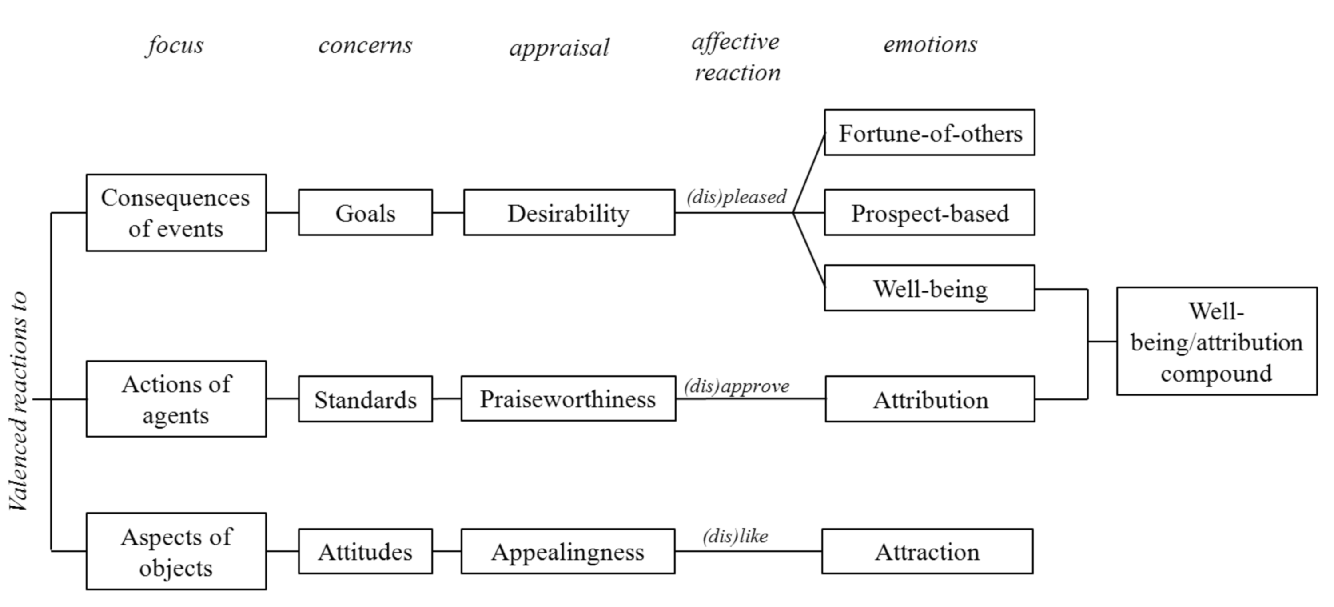
\includegraphics[width=\textwidth]{figure/occ.png}
  \caption{A simple visualization of OCC model \cite{occ:structure}.}
  \label{fig:occ-model}
\end{figure}

As shown in Figure \ref{fig:occ-model}, a person could alternatively have three
types of focus. These types of focus are the consequence of events, actions of
agents, and aspects of objects. A person evaluates the significance of the
causes behind these three types of focus based on her personal concerns. As a
result, an affective reaction will be elicited, resulting in an emotion. Various
combinations of the elements depicted in Figure \ref{fig:occ-model} create
specific patterns resulting in six main groups of emotions in which all emotion
types in a group share the same cognitive pattern (see Figure
\ref{fig:occ-structure}). Emotion groups are \textit{fortune-of-others,
prospect-based, well-being, attribution, well-being/attribution- compound}, and
\textit{attraction}. The OCC model introduces 22 emotion types. Each of these
emotions is introduced as a representative of a family of similar emotions
with various intensities (since relying on a list of discrete emotions that is
understood by everyone equally is impossible due to people's language barriers
and various interpretations of the actual words)\footnote{In stark contrast to
basic emotion theories discussed in Section \ref{sec:discrete-emotions}.}. For
instance,  while they all share the same eliciting conditions, happiness can be
referred to by many other emotion terms such as joy, cheerfulness, gladness and
delighted. Thus the emotion types used in the model (e.g., relief, love, pride,
and shame) are meant to represent an emotional experience rather than a lexical
taxonomy.

For instance, as shown in Figure \ref{fig:occ-model}, the appraisal criterion
for consequences of event’s is their \textit{desirability} for achieving one's
goals. This generates the affective reaction of being \textit{pleased} in
positive cases, or \textit{displeased} in negative ones. Figure
\ref{fig:occ-structure} shows the resulting emotion groups in OCC model such as
\textit{fortune-of-others} (e.g., gloating, pity), \textit{prospect-based}
(e.g., satisfaction, relief), and \textit{well-being} (e.g., joy, distress)
\cite{occ:structure}. The appraisal of the praiseworthiness of the actions of an
agent against one's personal standards, as well as the appealing aspects of
objects happens in the same way as shown in Figure \ref{fig:occ-model}.

\begin{figure}[tbh]
  \center
  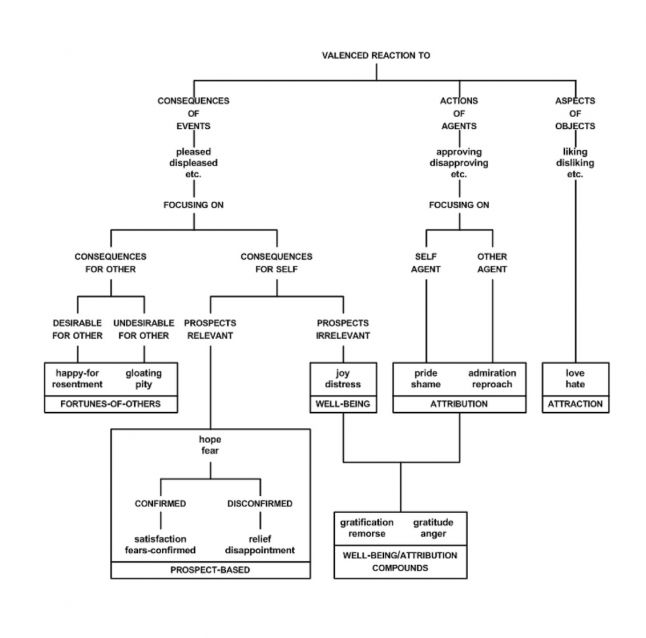
\includegraphics[width=0.978\textwidth]{figure/occ-structure.jpg}
  \caption{OCC taxonomy of emotion triggers and emotions \cite{occ:structure}.}
  \label{fig:occ-structure}
\end{figure}

Finally, the OCC model introduces some global variables of an emotion's
intensity to distinguish all types of emotions that a person could experience when
encountering events, agents or objects. These variables are as follows

\begin{enumerate}
	\item Sense of reality (representing the degree to which the event, agent or
	object in focus appear real to the person),

	\item Proximity variable (representing the psychological proximity of an event,
	agent or object),

	\item Unexpectedness (representing how surprising an event is for one, either
	positive or negative),

	\item Arousal (representing how arousing an event, agent or object is).
\end{enumerate}

\subsection{Other (Non-Appraisal) Computational Models}

\subsubsection{Constructivist (Dimensional) Emotion Theories}
\label{sec:dimensional-emotions}

The components and dimensions of emotions have been the subject of much
speculation since the 19th century. Dimensional models of emotion attempt to
conceptualize human emotions by defining where they lie in two or three
dimensions. Dimensional theories of emotion argue that emotions should be
conceptualized as points in a continuous dimensional space, rather than looking
at them as discrete entities \cite{carver:affect-behavior}
\cite{mehrabian-russell:pad} \cite{russell:core-affect}
\cite{watson:consensual-structure-mood}.

\begin{figure}[tbh]
  \center
  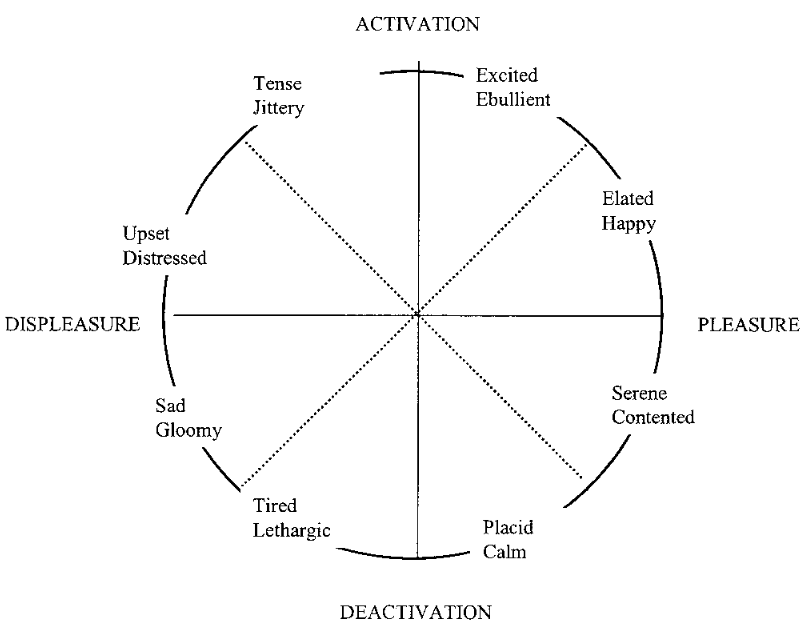
\includegraphics[width=.7\textwidth]{figure/core-affect.png}
  \caption{Russell's suggested affective states based on core affect
  \cite{russell:core-affect}.}
  \label{fig:core-affect}
\end{figure}

Two dimensions that are commonly proposed to describe emotions are valence and
physiological arousal \cite{arnold:emotion-personality}
\cite{lazarus:cognitive-theory-emotion} \cite{russell:circumplex-affect}. Models
based on dimensional theories introduce the emotion concept as a non-relational
construct summarizing a unique overall state of the individual. The models based
on dimensional theories contrast theories of basic emotion (see Section
\ref{sec:discrete-emotions}), which propose that different emotions arise from
separate neural systems \cite{posner:circumplex-affect}. Also, models based on
dimensional theories contrast appraisal theories, which propose that appraisals
are the relational constructs characterizing the relationship between one's
mental state and a specific stimulus. Many dimensional theories argue that
discrete emotion categories (e.g., sadness, fear and anger) have no ``reality''
in that there are no specific brain regions or functions that correspond to
specific emotions \cite{barrett:emotions-natural}. Therefore, dimensional
theories do not emphasize the term emotion.

\begin{figure}[tbh]
  \center
  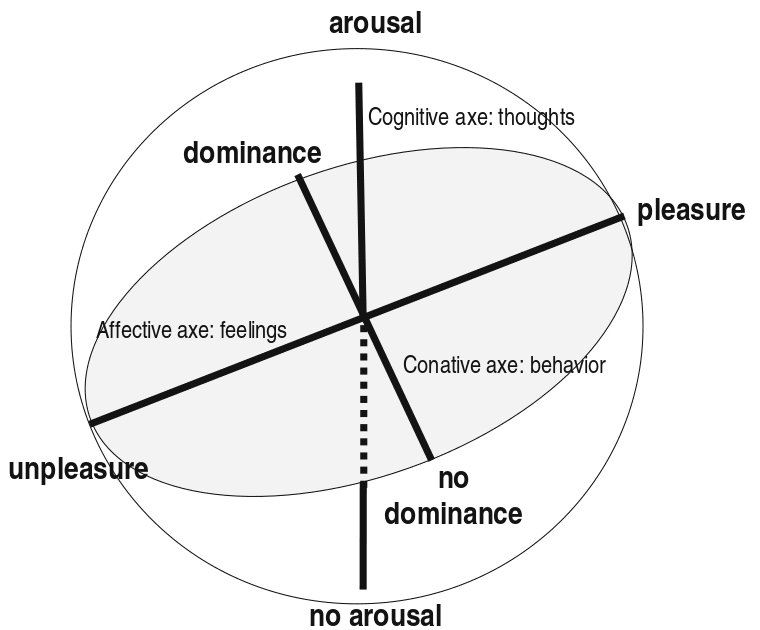
\includegraphics[width=.6\textwidth]{figure/dimensional2.png}
  \caption{Three dimensional model of pleasure, arousal and dominance as
  tripartite view of experience \cite{mehrabian:pad}.}
  \label{fig:pad}
\end{figure}

One of the most prominent two-dimensional models is Russell's circumplex model
\cite{russell:circumplex-affect}. Russell suggested that affective states are
all related to each other systematically through what is called core affect
\cite{russell:circumplex-affect,russell:core-affect} (see Figure
\ref{fig:core-affect}) and emotions are best described as a change in core
affect which, in turn, is describable as a point in a space of two dimensions.
One dimension is \textit{valence} or how good or bad objects and events are for
a being (ranging from pleasant to unpleasant). The other dimension is
\textit{arousal}, ranging from calm to excited. Russell put a number of
affective states around a circular space between those two dimensions (see
Figure \ref{fig:core-affect}) which is also known as \textit{circumplex},
representing the variety of core affects
\cite{russell:circumplex-affect,russell:core-affect}. Since sometimes
two-dimensional space cannot easily differentiate among emotions that share the
same values of arousal and valence, e.g., anger and fear (both characterized by
high arousal and negative valence), some of the dimensional models incorporate
valence and arousal as well as \textit{intensity}, or \textit{dominance} or
\textit{stance} dimensions. Many computational dimensional models build on the
three dimensional “PAD” model of Mehrabian and Russell
\cite{mehrabian-russell:pad} where these dimensions correspond to pleasure (a
measure of valence), arousal (indicating the level of affective activation) and
dominance (a measure of power or control). Figure \ref{fig:pad} shows these
three dimensions.

\begin{figure}[tbh]
  \center
  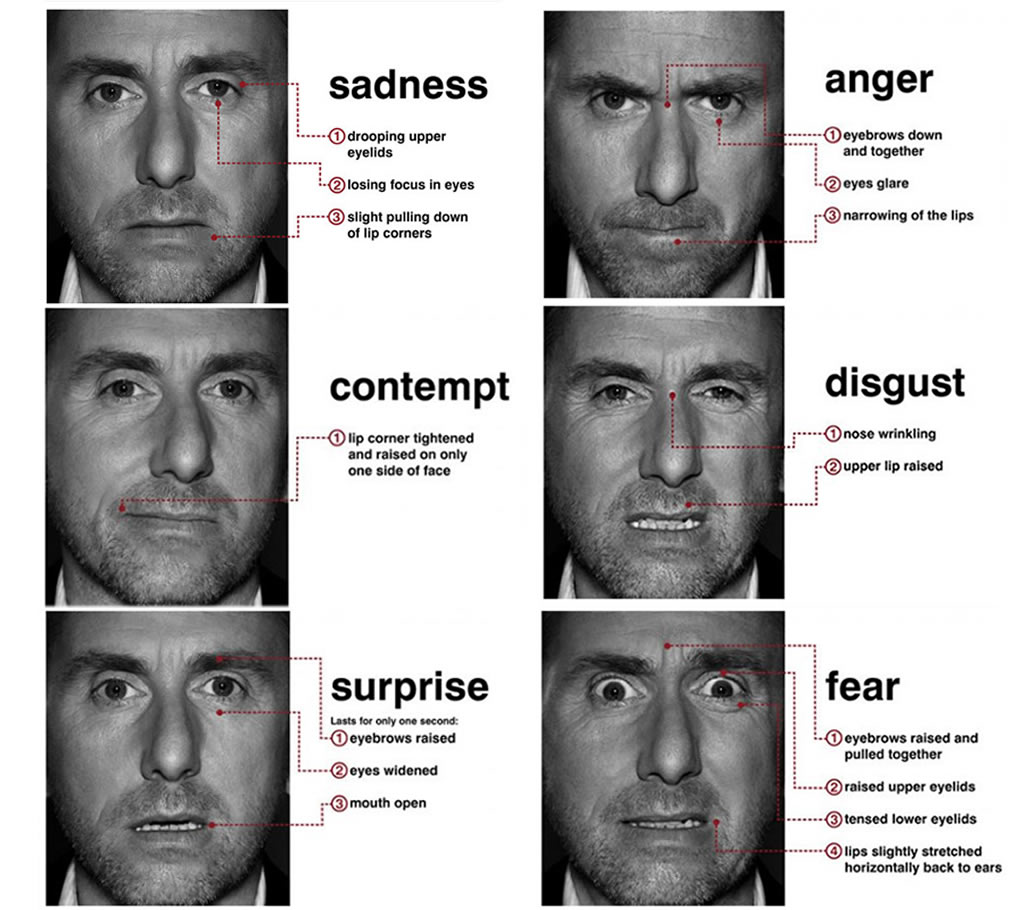
\includegraphics[width=.9\textwidth]{figure/basic-emotions.jpg}
  \caption{Basic emotions and corresponding expressions.}
  \label{fig:basic-emotions}
\end{figure}

\subsubsection{Basic (Discrete) Emotion Theories}
\label{sec:discrete-emotions}

Basic emotion theories are inspired by Tomkins' \cite{tomkins:affect}
rediscovery of Darwin's work
\cite{darwin:emotion-expression,hess:darwin-emotion} which were later developed
further by Ekman \cite{ekman:argument-emotions} and Izard
\cite{izard:human-emotions}. These theories emphasize a small set of discrete
and fundamental emotions. The underlying assumption of this approach is that
these emotions are mediated by associated neural circuitry, with a hardwired
component \cite{ekman:argument-emotions}. Different emotions are then
characterized by stable patterns of triggers, behavioral expression, and
associated distinct subjective experiences. The emotions addressed by these
theories are typically called the \textit{basic} emotions. Emotions including
happiness, sadness, fear, anger, surprise, and disgust are often considered to
comprise the most prototypical basic emotions \cite{ekman:argument-emotions}.
The theory of basic emotions holds that there is a set of emotions shared by all
humans that evolved to deal with ancestral life challenges
\cite{ekman:argument-emotions}. For instance, disgust evolved to address the
challenge of avoiding noxious stimuli, and fear evolved to address the challenge
of avoiding dangers. Because of the emphasis on discrete categories of states,
this approach is also termed the \textit{categorical} approach
\cite{panskepp:affective-neuroscience}. Much of the supporting evidence offered
for the theory comes from experiments that show how certain facial expressions
are universally associated with specific basic emotions, regardless of the
observer's cultural background. This universality has a production side and a
recognition side. On the production side, a particular emotional state is said
to elicit a facial expression comprised of a specific set of facial muscles. On
the recognition side, observers are able to infer the emotional state of the
person who expresses an emotion, due to the direct correspondence between
emotional states and the facial expressions they cause. Computational models
inspired by the basic emotions or discrete approach often focus on low-level
perceptual-motor tasks and encode a two-process view of emotion that argues for
a fast, automatic, undifferentiated emotional response and a slower, more
differentiated response that relies on higher level reasoning processes (e.g.,
\cite{armony:computational-modeling-emotion}). \\

% \subsection{Other Approaches}

There are other approaches that different researchers take based on their
emphasis on the applicability of emotions in their systems.

\subsubsection{Rational Approaches}

Rational approaches start from the question of what adaptive functions emotions
serve and then attempt to incorporate these functions into a model of
intelligence. Emotion, within this approach, is simply another set of processes
and constraints that have adaptive value. Models of this sort are most naturally
directed towards the goal of improving theories of artificial intelligence
\cite{anderson:newell-cognition} \cite{scheutz:affect-agent}
\cite{simon:motivation-emotion-cognition}.

\subsubsection{Communicative Approaches}

Communicative theories of emotion argue that emotion processes function as a
communicative system. They can function first, as a mechanism for informing
other individuals of one's mental state (thereby facilitating social
coordination), and second, as a mechanism for requesting/demanding changes in
the behavior of others. Communicative theories emphasize the
social-communicative function of expressions \cite{gratch:emotion-intention}.
Computational models inspired by communicative theories focus on machinery that
decides when an emotional expression can have a desired effect on a human
counterpart.

\subsection{Similarities and Differences}
\label{sec:comparison}

Different theoretical perspectives should not be viewed as competing for a
single truth. Instead, they should be seen as perspectives arising from
particular research areas (e.g., biological vs. social psychology), focusing on
different sets of affective phenomena, considering different levels of
resolution and fundamental components (e.g., emotions vs. appraisal variables).
These different perspectives provide different degrees of support for the
various processes of emotion, e.g., the componential theories provide extensive
details about cognitive appraisals \cite{hudlicka:guidelines-emotions}.
Therefore, this section provides a pairwise comparison between these fundamental
theories. Note that a separate pairwise comparison will not be provided for
appraisal vs.\,discrete (basic) emotion theories as the important points are
adequately covered in the comparisons presented below.

\subsubsection{Dimensional Vs. Discrete (Basic) Emotion Theories}

The fundamental assumption of the basic emotion theory is that a specific type
of event triggers a specific affect program corresponding to one of the basic
emotions and producing characteristic expression patterns and physiological
response configurations \cite{scherer:emotions-emergent}. Dimensional theories'
main criticism of basic emotions theory is based on the observation that
affective phenomena appear to be both qualitatively and quantitatively diverse.

Russell in \cite{russell:core-affect} argues the labels such as ``fear",
``anger'', ``happiness'' do not capture this diversity. For instance, one might
say: a) a person being chased by an assailant brandishing a knife, b) a person
who retreats from an insect moving across the floor, and c) a person who is
concerned they will never find a fulfilling career, are all in a state of
fear. On the basic emotions account, an emotional episode involves fixed
patterns of neurophysiological and facial expression changes in response to an
eliciting stimulus that are distinct between emotions, but are the same within
the same emotional category \cite{ekman:argument-emotions}. If this were the
case, one would expect that the three individuals described above would respond
to their eliciting stimuli in the same way, yet a similarity of behavioral
responses between these three cases seems unlikely. Dimensional theorists, in
contrast, would argue that the individuals in the above three cases are applying
the concept of fear to experience, despite the fact that each individual has a
unique core affect. While basic emotion theorists would hold that since all
three individuals are experiencing fear, they would perform the same behavioral
responses to the stimuli, dimensional theorists would argue this is not the
case, as each individual bears a core affective state that is distinguished from
the other two. For instance, the individual's arousal in response to an armed
assailant should be higher than the individual in response to an insect, as the
former case poses a threat to their life. As a result, the individual in the
first case would likely make every effort to escape from the assailant,
including trying to negotiate and plead with the assailant, while the individual
in the second case would be relatively less dedicated to escaping the insect. 

In sum, a dimensional theory is compatible with the differences in the
behavioral responses to eliciting stimuli, while basic emotions theory only
allows for a single fixed behavior of responses to a given emotion. Furthermore,
dimensional theories can represent instances of basic emotions (see Figure
\ref{fig:dimensional-discrete}), for example, fear elicited by a snake (green
rectangle), in terms of variation along affective dimensions, i.e., arousal and
valence.

\begin{figure}[tbh]
  \center
  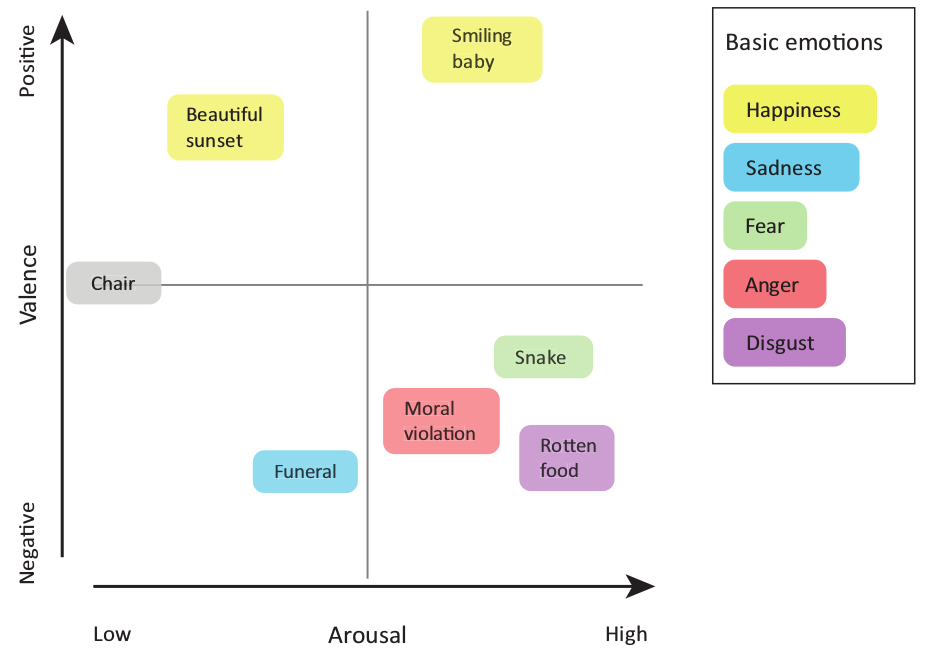
\includegraphics[width=.9\textwidth]{figure/dimensional-discrete.png}
  \caption{Representing basic emotions within a dimensional framework
  \cite{hamann:mapping-discrete-dimensional}.}
  \label{fig:dimensional-discrete}
\end{figure}

Also, basic emotion theory fails to account for affect that lacks
object-directedness \cite{russell:core-affect}. In the basic emotions approach,
an emotion is supposed to have an intentional object it is directed towards (e.g.,
being angry at someone, or being sad for someone). The dimensional theory argues
that emotion may not necessarily be aimed at a particular object. For instance,
an individual can experience a certain type of emotion (e.g., anger) without
knowing of anything in particular that has offended her. Dimensional models of
emotion are therefore capable of accounting for a wider range of affective
phenomena than basic emotions theory.

Another difference between dimensional and basic emotion theories is that the
basic emotion categorization of emotions captures facets of the experience of
an emotion not conveyed by the dimensional description, such as elicitation of a
facial expression of the emotion. In fact, this attribute of the basic
emotions theory is one of the major differences with all other emotion theories.
It is argued in basic emotion theory that basic emotions are hard-wired to their
corresponding facial expressions. Ekman, who elaborated the concept of basic
emotions, developed the \textit{Facial Action Coding System} (FACS) which
encodes movements of individual facial muscles and it is a common standard to
systematically categorize the physical expression of emotions
\cite{ekman:facial-movement}.

\subsubsection{Appraisal Vs. Dimensional Emotions Theories}

Dimensional theories struggle to adequately distinguish emotions because of the
existence of limited dimensions.

To compare the appraisal and dimensional theories of emotion, we argue that
there is a relationship between the dimensions in the dimensional theories of
emotion and the appraisal dimensions. For instance, the pleasure dimension
roughly maps onto appraisal dimensions that characterize the valence of an
appraisal-eliciting event, (e.g., intrinsic pleasantness --desirability--, or
goal congruence), dominance roughly maps onto the appraisal dimension of coping
potential, and arousal can be considered as a measure of intensity. However,
these dimensions and corresponding appraisal variables have quite different
meanings. Appraisal (as mentioned earlier) is a relational construct
characterizing the relationship between some specific object/event in the
environment and the individual's mental constructs including beliefs, motives
and intentions. Also, several appraisals may be simultaneously active, whereas
emotions in dimensional emotion theory are non-relational constructs, each
summarizing a unique overall state of the individual.

Furthermore, dimensional emotion theories emphasize different components of
emotion than appraisal theories and link these components quite differently.
In contrast to appraisal theories, dimensional emotion theories do not address
affect's antecedents in detail. Dimensional theorists question the tight causal
linkage between appraisal and emotion that is central to appraisal accounts. As
mentioned earlier, dimensional theorists believe that the emotion is not
necessarily about some object (as in ``I am angry \underline{at him}''). In such
theories, many factors may contribute to a change in emotion including
intentional judgments (e.g., appraisal). However, in dimensional emotion
theories, the link between any preceding intentional meaning and emotion is
broken and most of the time cannot be recovered correctly. For example, Russell
argues for the following sequence: some external event occurs (e.g., a bear
walks out of the forest), it is perceived in terms of its affective quality;
this perception results in a crucial change in core affect; this change is
attributed to some ``object" (e.g., the bear); and only then is the object
cognitively appraised in terms of its goal relevance, causal antecedents and
future prospects \cite{marsella:computational-models}.

We can also compare dimensional emotion theories to the OCC model as a cognitive
appraisal model. The major similarity between these two models is that they both
consider emotions to descend from valenced reactions to the stimuli.
Furthermore, they acknowledge the role of arousal in determining emotional
reactions. As mentioned in Section \ref{sec:dimensional-emotions}, Russell
considered arousal as one of the two key dimensions of emotions which could be
used to partially discriminate emotional states
\cite{russell:circumplex-affect}. In a different manner, the OCC model
recognizes arousal as a necessary condition for eliciting emotions, and regards
arousal as a major determinant of the elicited emotion's intensity which
distinguishes among various emotions of a particular type (e.g., fearful versus
scared). In \cite{scherer:what-emotions} Scherer speculates that the arousal
dimension in dimensional models gives little information about the underlying
appraisal of the elicited emotion and proposes to replace it with coping
potential, which is an appraisal dimension referring to the individual's
perceived control in a given situation.

Models based on dimensional emotion theories pursue the idea of eliciting an
emotion according to the joint features in circumplex space (2D or 3D -- see
Section \ref{sec:dimensional-emotions}), while OCC or other models of appraisal
theory are based on patterns of antecedents of emotions. This is the fundamental
difference between OCC, or appraisal theories in general, and the circumplex
approach of Russell \cite{russell:circumplex-affect} or Mehrabian's PAD model
\cite{mehrabian:pad,mehrabian-russell:pad}. Also, models based on appraisal
theory of emotions employ causation, attribution and eliciting conditions in
order to distinguish emotions, while the eliciting conditions are not directly
accessible from a dimensional approach. A dimensional model may fall short in
establishing why certain emotions are elicited. However, when the objective is
to identify the generated emotions and their level of pleasantness and
intensity, a circumplex model presents an excellent opportunity
\cite{ahmadpour:occ-dimensional-comparison}.

\begin{figure}[tbh]
  \center
  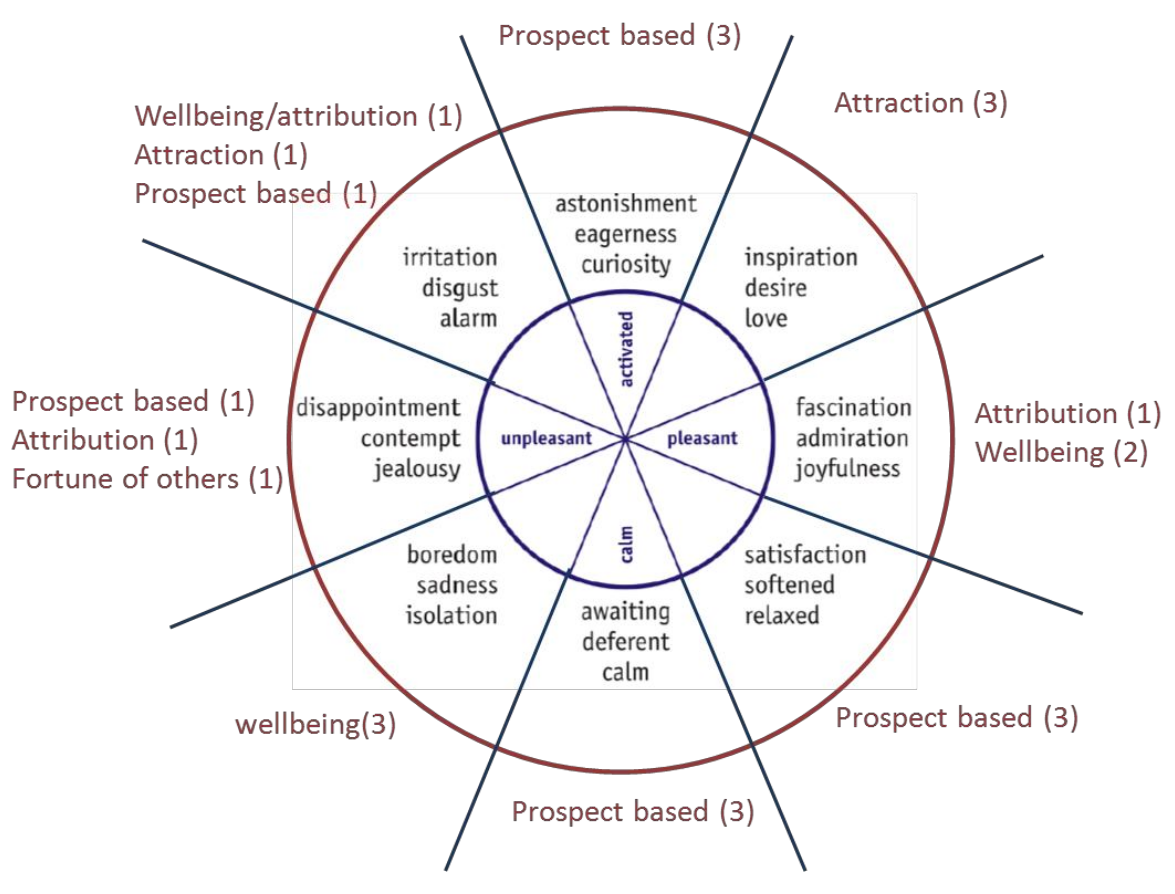
\includegraphics[width=.9\textwidth]{figure/occ-circumplex-mapping.png}
  \caption{A rough projection of emotion groups of OCC on the circumplex of
  affect \cite{ahmadpour:occ-dimensional-comparison}.}
  \label{fig:occ-circumplex}
\end{figure}

Finally, we consider how a model based on dimensional emotions (i.e., Russell's
2D circumplex) relates to a cognitive model based on appraisal theory (i.e.,
OCC). Figure \ref{fig:occ-circumplex} shows the relationship between Russell's
circumplex and the OCC model in terms of the categorization of actual emotions.
The number of emotions in a section of Russell's circumplex that fall into an
emotion group of OCC is shown in parentheses. For instance, all three emotions
in the top section (highly excited, neutrally valenced emotions) fall into
prospect-based emotion group. Or, as another example, emotions in the left
section (neutral arousal value, negative valenced emotions) make a one to one
relationship between disappointment and the prospect based emotion group,
contempt and attribution emotion group, and jealousy and fortune of others
emotion group (hence number (1) is indicated in front of each).

\subsection{Applications in Autonomous Agents and Robots}
\label{sec:applications}

There are many research areas, including robotics and autonomous agents, that
employ the structure and/or functions of emotions in their work with a variety
of reasons for modeling emotions \cite{wehrle:motivations-modeling-emotion}.
Some of this work is inspired by specific psychological theories, while some are
freely using the concept of emotion without a theoretical grounding in social
sciences; some are using a combination of concepts from different psychological
theories. For instance, in PECS \cite{urban:pecs}, which is designed for
modeling human behaviors, the agent architecture is not based on any specific
social or psychological emotion theory. In fact, it is intentionally designed
and described in a way which enables the integration of a variety of theories.
The PECS' design enables an integrative modeling of physical, emotional,
cognitive and social influences within a component-oriented agent architecture.
Also, in \cite{miranda:teamwork-multiagent-system} the computational
architecture, which is designed to provide information about the possible
overall behavior of a work team, is not based any specific theory. As mentioned
earlier, some researchers apply combinations of emotion theories in their work
\cite{kiryazov:modeling-appraisal-pad}. For instance, in
\cite{canamero:designing-activity-selection} Ca$\tilde{n}$amero shows how an
agent can use emotions for activity selection while taking into account both
dimensional and discrete approaches in an action selection mechanism.

We can also see the application of emotion theories in designing companion
robots capable of expressing emotions and social behaviors, as well as robots
which can convey certain types of emotion products, e.g., empathy
\cite{breazeal:expressive-behavior} \cite{leite:empathy-hri}
\cite{paiva:emotion-modeling} \cite{shayganfar:methodology}. Robots also use
emotion theories for automatic affect recognition using different modalities
\cite{hegel:empathic-robot} \cite{zeng:affect-recognition}. Moreover, in some
work, researchers have explored the user's affective state as a mechanism to
adapt the robot's behaviors during the interaction
\cite{breazeal:sociable-robot} \cite{liu:affect-robot-behavior}.\\

\textbf{Applications of Appraisal Theory} -- The emphasis of models derived from
appraisal theories of emotion is on making appraisal the central process.
Computational appraisal models often exploit elaborate mechanisms for deriving
appraisal variables such as decision-theoretic plans
\cite{gratch:domain-independent} \cite{marsella:ema-process-model}, reactive
plans \cite{rank:appraisal-story-world} \cite{neal:modeling-antecedents}
\cite{staller:emotion-social-norm}, Markov-decision processes
\cite{elnasr:flame} \cite{si:modeling-appraisal-tom-journal}, or detailed
cognitive models \cite{marinier:behavior-emotion}. However, emotion itself is
sometimes treated less elaborately, simply as a label to which behavior can be
attached \cite{elliott:affective-reasoner}. Appraisal is usually modeled as the
cause of emotion being derived via simple rules applied to a set of appraisal
variables.

Computational appraisal models have been applied to a variety of uses including
contributions to psychology, robotics, AI, and HCI. For instance, Marsella and
Gratch have used EMA \cite{marsella:ema-process-model} to generate specific
predictions about how human subjects will appraise and cope with emotional
situations and argue that empirical tests of these predictions have implications
for psychological appraisal theory \cite{gratch:assessing-appraisal}
\cite{marsella:assessing-coping}. There are other examples in artificial
intelligence and robotics of applying appraisal theory
\cite{adam:bdi-emotional-companion} \cite{kim:model-hri-appraisal}
\cite{marsella:ema-process-model}. In robotics, appraisal theory has been used
to establish and maintain a better interaction between a robot and a human. For
instance in \cite{kim:model-hri-appraisal} researchers use a computational model
of emotion generation based on appraisal theory to have a positive human-robot
interaction experience. In \cite{sander:systems-approach-appraisal} the authors
describe a system approach to appraisal processes based on Scherer's work on
appraisal and the CPM \cite{scherer:nature-function-emotion}. They show how the
temporal unfolding of emotions can be experimentally tested. They also lay out a
general domain-independent computational model of appraisal and coping. In
\cite{vogiatzis:robot-museum} researchers consider their robot, INDIGO's,
emotion, speech and facial expressions as key features to establish effective
communication between the robot and a human during their interaction. They apply
concepts of appraisal theory in INDIGO's emotion modeling. MAGGIE, a sociable
robot, also applies an appraisal theory of emotions to consider fear in its
decision making system \cite{castro:autonomous-robot-fear}. Velasquez developed
Cathexis, which is a distributed computational model for generation of emotions
and their influence in the behavior of the autonomous agents
\cite{velasquez:emotions-motivations-agents}. The emotion model in this work is
based on Roseman's work on appraisal theory. Marinier and Laird in
\cite{marinier:emotion-reinforcement} focus on the functional benefits of
emotion in a cognitive system. In this work, they integrate their emotion theory
(which is based on appraisal theory) with the Soar cognitive architecture, and
use emotional feedback to drive reinforcement learning. In
\cite{hudlicka:emotinos-reasons} Hudlicka provides a generic mechanism mediating
the affective influences on cognition based on cognitive appraisal. This model
is implemented within a domain-independent cognitive-affective architecture
(MAMAID).

In the virtual agents community, empathy is a research topic that has received
much attention in the last decade \cite{brave:emotion-hci}
\cite{scott:modeling-empathy-agent} \cite{paiva:agent-care}
\cite{prendinger:empathic-companion} \cite{bickmore:longterm-relationship}. In
\cite{pontier:women-robot-men} researchers developed an agent with the
capability of affective decision-making based on appraisal theory to establish a
relationship with its users. Then, they compared the performance of their agent
with a human (based on a WoZ study) in a speed-dating experiment. In HCI,
appraisal theory has been primarily used for the creation of interactive
characters that exhibit emotions in order to make characters more believable
\cite{neal:believable-agents}, more realistic \cite{mao:social-causality}
\cite{traum:negotiation-teams-training}, more capable of understanding human
motivational states \cite{conati:evaluating-student-affect} or more able to
induce desirable social effects in human users \cite{paiva:learning-feeling}.

\textbf{Applications of Dimensional Theory} -- The emphasis of models influenced
by dimensional theories is on processes associated with core affect which is
usually represented as a continuous time-varying process, and can be represented
at a given time by a point in a 2D or 3D-space as a response to the eliciting
events. Generally, there are detailed mechanisms in computational dimensional
models which determine how this point changes over time, e.g., decay to some
resting state, and incorporating the impact of dispositional tendencies such as
personality or temperament \cite{gebhard:alma}
\cite{marsella:computational-models}. Models based on dimensional theories have
also been used in robotics. For instance, researchers in
\cite{lim:mei-motherese-ei} apply PAD's three-dimensional space to rate the
pleasure, arousal and dominance of their Multimodal Emotional Intelligence robot
(MEI) in each interaction with human subjects. Their goal is to introduce the
first steps in MEI which can understand and express emotions in voice, gesture
and gait. In \cite{zhang:service-robot-dimensional} researchers want to
understand the effect of different interface features for a service robot. They
use valence and arousal dimensions in their questionnaires to assess the
perceived anthropomorphism of their service robot by subjects. In
\cite{klug:emotion-based-hri} researchers introduce the implementation of a
dynamic personality for a robot based on a dimensional emotion model. They use
WASABI's architecture \cite{becker:wasabi,becker:wasabi-description} as their
emotional model. In \cite{lisetti:affect-socially-intelligent} Lisetti describes
an affective knowledge representation scheme to be used in the design of a
socially intelligent artificial agent. Lisetti uses the valence-arousal two
dimensional model of emotion in this work. This model has been applied in an
emotion-based architecture of Lisetti's autonomous robots as well as a
multimodal affective user interface agent. ROMAN, an expressive robotic head,
uses a behavior-based emotional control architecture. The approach to the
emotional component of the architecture is based on the dimensional emotion
theory \cite{hirth:roman}.

\textbf{Comparison of Applications of Emotion Theories} -- Researchers often use
computational dimensional models for behavior generation of animated characters.
The reason might be because it is easier to translate emotions to a limited
number of dimensions that can be readily mapped to continuous features of
behavior such as the spatial extent of a facial expression. For example, PAD
models describe all behavior in terms of only three dimensions of pleasure,
arousal and dominance, whereas researchers using appraisal models whould need to
either associate each behavior with a large number of appraisal variables
\cite{scherer:expression-appraisal}
\cite{smith:computational-facial-expression}, or try to map appraisal variables
into a limited and small number of discrete expressions
\cite{elliott:affective-reasoner}. For a similar reason, dimensional models are
also frequently used as a representational framework for systems that attempt to
recognize human emotional behavior. There is some evidence that they may better
discriminate user affective states than approaches that rely on discrete labels
\cite{barrett:emotions-natural}.

There is also a relationship between dimensional and appraisal theories. Some of
the computational models of emotion that incorporate dimensional theories have
viewed appraisal as the mechanism that initiates changes to core affect. For
instance, ALMA \cite{gebhard:alma} includes OCC inspired appraisal rules
\cite{occ:structure}, and WASABI \cite{becker:wasabi} includes appraisal
processes inspired by Scherer's sequential-checking theory into a PAD-based
emotion model. Moreover, some computational models explore how core affect in
dimensional models can influence cognitive processes. For example, HOTCO 2
\cite{thagard:emotional-coherence} allows explanations to be biased by
dimensional affect \cite{marsella:computational-models}.

\section{Affect and Motives}
\label{sec:affect-motives}
Motives are essential mental components in decision-making procedures and
applying them in an affect-driven collaborative agent is part of this thesis'
contribution. In this section, we review related work on computational models
of motivation and discuss the nature of motives. We also explain three of the
important social motives which will be used in our work. Finally, we discuss
how humans' beliefs, emotions and motives are related and influence each other. 

Motivation principles and mechanisms, as the reasons behind one's intentions and
actions, and the influences of motives on cognition have been discussed in
philosophy, neuroscience, psychology and artificial intelligence
\cite{bach:motivaitional-system-ai, berridge:motivation-concepts-neuroscience,
brody:motivation-goal-action, simon:motivation-emotion-cognition,
sloman:motivation}. There are several examples in AI of computational models for
different psychological theories of motivation. Bach's MicroPsi agent
architecture describes the interaction of emotion, motivation and cognition of
agents based on Dietrich D$\ddot{o}$rner's Psi theory
\cite{bach:micropsi-agent-architecture, bach:psi, bach:motivaitional-system-ai,
bach:next-generation-micropsi}. Merrick and Shafi provide a computational model
for motivation based on Henry Murray's theory
\cite{murray:personality-exploration} describing the three important social
motivations of \textit{achievement, affiliation} and \textit{power}. They focus
on the role of motivation in a goal-selection mechanism
\cite{merrick:acheievement-affiliation-power}. There are other examples focusing
on the impact of motives on different cognitive processes in robots and
artificial agents \cite{breazeal:motivation-regulating-hri,
dolores:socially-emotional, deSevin:motivational-model-agent,
sellers:comprehensive-emotion-theory, velasquez:emotions-motivations-agents,
wright:implementation-agent-architecture}. The motivation mechanism in our work
is inspired by Murray's theory and Bach's approach on D$\ddot{o}$rner's theory.
It is focused on the role of motives in cognitive processes, e.g.,
intention formation in coping, during collaboration, which will be discussed in
Chapters \ref{ch:amct} and \ref{ch:appraisals}.

\subsection{Motives}

A motive consists of an urge (that is, a need indicating a demand) and a goal
that is related to this urge \cite{bach:psi}. Motives shape cognition and
behavior \cite{schultheiss:implicit-motive}. To be motivated means to be moved
to do something \cite{ryan:intrinsic-extrinsic-motivations}. Motives direct
behaviors towards particular goals, which makes the agent more persistent in
actions it takes. They also affect cognitive processes by increasing the level
of attention. Motive, as the outcome of the motivation process, initiates,
directs and maintains goal-oriented behaviors.

Motives are goal-driven and they move the agent towards the attainment of
corresponding sets of intentions. In other words, motives as an essential part
of affect can lead the agent to empower an intention. They are essentially
mechanisms that in light of beliefs tend to produce, modify or select between
actions and their reciprocal intentions. Some of motives are transient, like
helping the Astronaut to hold the panel, while some are long term, like reaching
to the shared goal of the collaboration in our ongoing example, installing
solar panels and satisfying the Astronaut's needs in the field constitutes
the shared goal (see Section \ref{sec:example-scenario}).

\subsection{Motivation Theory}
\label{section-motivation-theory}

There are several prominent motivation theories in psychology
\cite{beck:motivation, graham:motivation, laming:understanding-motivation}, some
of which have received attention as the basis for computational models. In
\cite{murray:personality-exploration}, Murray described and studied 20 different
human motives, of which three have received attention in psychology and
artificial intelligence as social motives
\cite{merrick:acheievement-affiliation-power,
zurbriggen:linking-motives-emotions}. {\color{red}Our work on motives has been
inspired by some of these work in the literature. However, we have developed our
own motive types and their computational models (see Section
\ref{sec:motivation_mechanism}).} The following is a brief description of these
three social motives, \textit{achievement, affiliation} and \textit{power}
\cite{atkinson:motives-action-society,zurbriggen:linking-motives-emotions}
which will be used in this thesis:

\begin{itemize}
  \item \textbf{Achievement motivation:}
  Achievement motivation drives humans to strive for excellence by improving on
  personal and societal standards of performance. It involves a concern for
  excellence, for doing one's best. In artificial agents, achievement
  motivation has potential roles in focusing agent behavior and driving the
  acquisition of competence.
  
  \item \textbf{Affiliation motivation:}
  Affiliation refers to a class of social interactions that seek contact with
  formerly unknown or little known individuals and maintain contact with those
  individuals in a manner that both parties experience as satisfying,
  stimulating, and enriching. It involves a concern with developing friendly
  connections with others through the two contrasting emotional components of
  hope of affiliation and fear of rejection. These two components become more
  crucial in the collaboration domain due to the importance of social emotions
  and their impact on beliefs and intentions.
  
  \item \textbf{Power motivation:}
  Power can be described as a domain specific relationship between two
  individuals, characterized by the asymmetric distribution of social
  competence, access to resources, or social status. It involves concern with
  having an impact on other people or on the world at large. There are different
  aspects of fear or avoidance of power which channel and moderate the
  expression of power into socially acceptable behavior, working as inhibitions
  to unseemly tendencies. Power motivation can be considered with respect to the
  probability of success which makes it relevant to the cognitive appraisal of
  emotions during collaboration.
\end{itemize}

In \cite{zurbriggen:linking-motives-emotions} it is shown that success of a
power goal is associated with anger, confusion and disgust; success at an
affiliation goal is associated with interest, happiness and feeling loved; and
success at an achievement goal is associated with interest, surprise, happiness,
excitement and a sense of focus. In other words, succeeding at a particular
motive is associated with experiencing particular emotions.

\section{Theory of Mind}
\label{section-tom-bg}

Theory of Mind (ToM), as a crucial component in human's social interaction,
plays an important role in our computational model. It concerns one's beliefs
about others as intentional agents. Beside the immediate effect, an individual's
action also depends on her beliefs about other's perception of that action as
well as the reaction they take. In this thesis, we use the ToM concept whenever
the agent needs to anticipate a human's mental states. We will also use the
term \textit{user model} as a standard collection of properties to describe
others.

The concept of theory of mind has received much attention in social psychology
and artificial intelligence. Eligio et al.\,explore what collaborators
understand about each other's emotions and conclude that being aware of each
other's emotions helps collaborators to improve their performance
\cite{eligio:emotion-understanding-collaboration}. Fussell and Kraus discuss the
importance of perspective taking in a successful communication in a social
setting \cite{fussell:knowledge-coordination-communication}. Scassellati
discusses the importance of attribution of beliefs, goals and desires to others.
He presents two psychological theories on the development of theory of mind in
humans and their potential application in building robots with similar
capabilities \cite{scassellati:tom-humanoid-robot}. Hiatt and Trafton present a
cognitive model which borrows mechanisms from three different postulates of
theory of mind and show that their model produces behaviors in accordance with
various theories of experiences \cite{hiatt:cognitive-model-tom}. Si, Marsella
and Pynadath discuss PsychSim, an implemented multi-agent-based simulation tool
for modeling social interaction, which has its own beliefs about its environment
and a recursive model of other agents \cite{pynadath:modeling-tom-appraisal}.
They also investigate the computational modeling of appraisal in a multi-agent
decision-theoretic framework using POMDP based agents
\cite{si:modeling-appraisal-tom, si:modeling-appraisal-tom-journal}. Since
applying the concept of theory of mind is crucial in social interaction and
collaboration, this thesis includes a simple ToM mechanism inspired by this
previous work.

\section{Conclusion}

In this chapter, we started by defining the concept of collaboration based
on Grosz and Sidner's work \cite{grosz:plans-discourse}, and listed a number of
collaboration properties. Then, we provided the background of two prominent
computational theories of collaboration which helped develop a better
understanding of the theories and how they relate to each other. Next, we
presented the SharedPlans theory and its main properties, e.g., partial shared
plan, recipe, and two notions of intention. Afterwards, we discussed the key
concepts of the Joint Intentions theory including joint commitment and joint
intention. Then, we continued with the hybrid approach of modeling collaboration
and discussed one of the most well-established models, STEAM. We also briefly
mentioned some other approaches. Later, we presented two different lists to
compare similarities and differences between SharedPlans and Joint Intentions
collaboration theories. We ended this document with different categories of
applications of these theories in agent/robot and human collaboration areas.

We believe the SharedPlans and Joint Intentions collaboration theories are the
most well-defined and well-established theories in computer science. We found
SharedPlans theory more convincing than the other major and subordinate
approaches, with respect to its inclusive explanation of the collaboration
structure and its association to discourse analysis which directly improves the
communicative aspects of a collaboration theory. We also understand the value of
Joint Intentions theory due to its clarity and closeness to the foundations of
collaboration concepts. These specifications of the Joint Intentions theory can
make it applicable in multi-agent system designs and human-robot collaboration.
We also consider hybrid approaches valuable, such as STEAM, if they clearly
understand drawbacks with existing theories and successfully achieve better
collaborative agents by infusing different concepts from different theories.
Although all these theories are well-defined and properly introduce
collaboration concepts, they mostly explain the structure of a collaboration and
they lack the underlying domain-independent processes with which collaborative
procedures could be defined more systematically and effectively in different
applications.

We have also discussed the description of affective computing and the importance
of the concept of emotion in general and in social context. We reviewed the
importance of communicating emotions as well as emotions' social functions.
Then, we provided some examples of agents and robots using artificial emotions
in their decision making process. We also briefly provided a few examples of
cognitive architectures producing different aspects of behaviors in robotics.

There are major theories of emotions explaining the concept of emotion. We
discussed these major theories in detail separately, providing their
psychological background and underlying concepts. Following the explanation of
these theories, we were able to discuss the similarities and differences between
these major theories. Finally, we provided applications of these theories in
robotics and AI.

We have developed our work based on computational models of emotions, it is
good to follow well-established (in comparison with others) theoretical
foundations. These theories can be a guideline for our computational models, and
they can explain more details of the structure or the processes involved in
affective situations. However, we do not necessarily think that the
computational models must exactly follow only one theory and its descriptions.
Meaning, different aspects of models can represent different theories. For
instance, appraisal theory is a good representation of the interpretive aspect
of emotions and basic emotion theories provide detailed systematic methods for
expressive application. More importantly, we believe the interpersonal functions
of emotions should be our first concern and we should try to relate them to the
structure of our domain, i.e., collaboration. In conclusion, we can see the
importance of interpretive, communicative and regulatory aspects of emotion
functions in this proposed work.

\chapter{Affective Motivational Collaboration Theory}
\label{ch:amct}
\vspace*{-5mm}
Current computational collaboration theories specify the structure of
collaborative activities, but are weak on the underlying processes that generate
and maintain these structures. {\color{red}In addition, current computational
models of emotion (specifically appraisal models) provide antecedents (e.g.,
beliefs and goals) of appraisal processes and clearly distinguish between
different appraisals, but do not describe the differences of appraisal in a
collaboration context.} We argue that emotions are crucial to these underlying
processes and we have developed a new computational theory, called
\textit{Affective Motivational Collaboration} theory, that combines
emotion-based processes, such as appraisal and coping, with collaboration
processes, such as planning, in a single unified framework. {\color{red}In this
chapter, we provide a general argument about our AMC theory, major functions of
emotions that can be applied in collaboration context, as well as the components
in our architecture and how each component (mechanism) deals with the events in
a collaborative environment. We also provide the definition of elements of
mental state and their attributes. Later in Chapter \ref{ch:appraisals}, we use
all these information in the new algorithms we have developed, e.g., appraisal
processes, as part of a new overall computational model.}

This work is implemented to build robots capable of generating and recognizing
emotions in order to be better collaborators. We have investigated the mutual
influences of affective and collaborative processes in a cognitive theory to
support interaction between humans and robots or virtual agents. We build
primarily on the \textit{cognitive appraisal} theory of emotions and the
\textit{SharedPlans} theory of collaboration to investigate the structure,
fundamental processes and functions of emotions in a collaboration.

Although existing collaboration theories specify the important elements of a
collaboration structure, the underlying processes required to dynamically
create, use, and maintain the elements of this structure are largely
unexplained. For instance, a general mechanism has yet to be developed that
allows an agent to effectively integrate the influence of its collaborator's
perceived or anticipated emotions into its own cognitive mechanisms to prevent
shared task failures while maintaining collaborative behavior. Therefore, a
process view of collaboration must include certain key elements. It should
inherently involve social interactions since all collaborations occur between
social agents, and it should contain a means of modifying the content of the
social interaction as the collaboration unfolds. The underlying processes of
emotions possess these two properties, and social functions of emotions explain
some aspects of the underlying processes in collaboration.

There is also a communicative aspect of emotions. For instance, emotions are
often intended to convey information to others \cite{goffman:self-presentation}.
Emotions are also involved in verbal behaviors. For instance, an utterance can
include both content and relational meaning. An emotion might appear to be
elicited by the content of the utterance, but in fact be an individual's
response to the relational meaning \cite{planalp:communicating-emotion}. The
interpretation of these relational meanings are handled by the appraisal of
events. Appraisal processes give us a way to view emotion as social
\cite{hooft:sharing-emotions}. Meaning is created by an individual's social
experiences in the social world, and individuals communicate these meanings
through utterances. Consequently, the meaning of these utterances and the
emotional communication change the dynamic of social interactions. A successful
and effective emotional communication necessitates ongoing reciprocal
adjustments between interactants that can happen based on interpretation of each
other's behaviors \cite{parkinson:emotion-social-interaction}. This adjustment
procedure requires a baseline and an assessment procedure. While the components
of the collaboration structure, e.g., shared plan, provide the baseline,
emotion-related processes (e.g., appraisal) provide the assessment procedure.

\textit{Affective Motivational Collaboration} theory is about the interpretation
and prediction of the observable behaviors in a dyadic collaborative
interaction. The theory focuses on the processes regulated by emotional states.
These observable behaviors represent the outcome of processes related to the
interpretation of the self's relationship to the collaborative environment.
The processes are triggered by the events occurring in the collaborative
environment. Thus, \textit{Affective Motivational Collaboration} theory explains
how emotions regulate the underlying processes when the events occur during
collaboration.

Emotion-regulated processes operate based on the self's mental states including,
the anticipated mental states of the other. These mental states include beliefs,
intentions, goals, motives and emotion instances. Each of these mental states
possesses multiple attributes impacting the underlying processes of
collaboration and ultimately the relation between cognition and behavior of the
agent. The nature of these attributes will be discussed in Section
\ref{sec:mental-states-attributes}.

\begin{figure}[h!] 
  \centering
  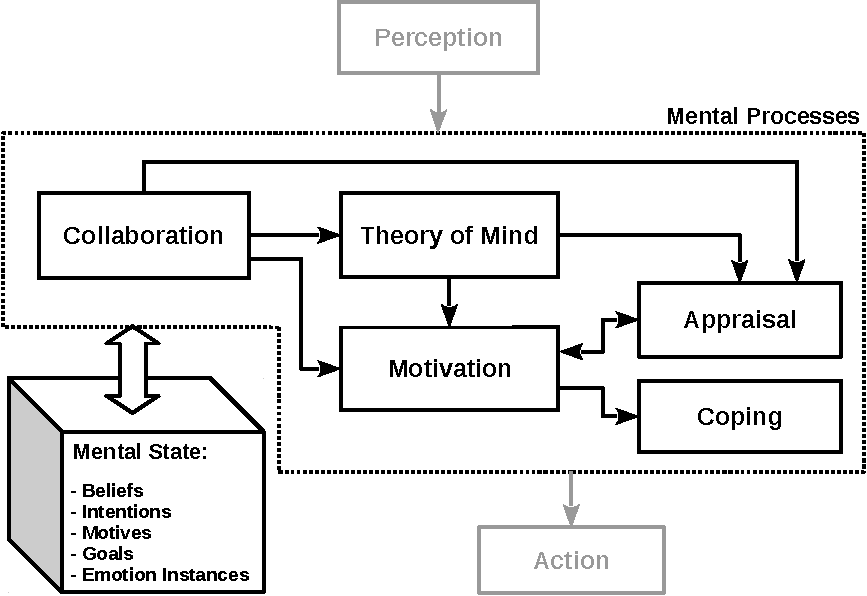
\includegraphics[scale=1]{figure/theory-general-croped.pdf}
  \caption{Primary influence of mechanisms in \textit{Affective Motivational
  Collaboration Theory}.}
  \label{fig:theory}
  \vspace*{-2mm}
\end{figure}

There are several theories discussed in Chapter \ref{ch:background}, which
describe the underlying structure of a collaboration based on mental states of
the collaborators. The collaboration structure of \textit{Affective Motivational
Collaboration Theory} is based on the SharedPlans theory
\cite{grosz:shared-plans}. \textit{Affective Motivational Collaboration} theory
focuses on the processes that generate, maintain and update this structure
based on mental states. The collaboration structure is important because social
agents/robots ultimately need to co-exist with humans, and therefore need to
consider humans' mental states as well as their own internal states and
operational goals.

\section{Overview of Mechanisms}

{\color{red}In this section, we introduce all mechanisms and the connections
between them in our architecture. The \textit{perception} and the
\textit{Action} mechanisms are only the source (to produce sensory information)
and the sink (to show proper behavior) of data in our architecture. These two
mechanisms function based on the same events introduced in Section
\ref{sec:events}.}

{\color{red}The \textit{Appraisal} and \textit{Coping} mechanisms are two major
mechanisms in our computational framework that are tightly coupled. The
Appraisal mechanism is responsible for evaluating changes in the self's Mental
States, the anticipated Mental States of the other, and the state of the
collaboration environment. Consequently, the Appraisal mechanism is connected to
a) the Theory of Mind mechanism, to serve as an evaluator whenever the self
applies the Appraisal mechanism to the mental states attributed to the human
collaborator, b) the Collaboration mechanism, to interpret the progress and
changes in the collaboration plan and associated Mental States, and to make
changes to the shared plan if required, c) the Motivation mechanism, to generate
and assess the self's new goal-driven motives whenever a new motive or intention
is required, e.g., following the failure of a task, and d) the Perception
mechanism, to interpret the external events from the collaboration environment.
In general, our appraisal algorithms are developed based on the data available
in a collaboration structure. This feature makes our algorithms unique and
different than other computational appraisal models. The details about our
algorithms are provided in Section \ref{sec:appraisal}. The Coping mechanism
provides the self with different coping strategies associated with changes in
the self's mental states with respect to the state of the collaboration. In
other words, the Coping mechanism produces cognitive responses by forming new
intentions based on the appraisal patterns. The Coping mechanism is also
inspired by other work; however, it is developed to enable an agent to cope with
the events in a collaborative environment which also distinguishes our work from
other computational models of coping. Details about our coping mechanism can be
found in Section \ref{sec:coping-mechanism}.}

The \textit{Motivation} mechanism provides motives to influence the coping
process in terms of the collaborative agent's or the human collaborator's needs.
The Motivation mechanism uses the Appraisal mechanism to compute attributes (see
Section \ref{sec:mental-states-attributes}) of competing motives. Also, the
Motivation mechanism can serve the Theory of Mind mechanism by helping the self
to infer the motive behind the other's current action. Moreover, the Motivation
mechanism applies the beliefs associated with the Appraisal mechanism to
generate and compare a new set of motives related to the status of the
collaboration. The outcome of the Motivation mechanism is involved in forming a
new intention to cope with the current event. As a result, the self can take an
action based on the new intention to sustain the collaboration progress.

The \textit{Theory of Mind} mechanism is responsible for inferring a model of
the other's anticipated Mental States. The self will progressively update this
model during the collaboration. The refinement of this model helps the self to
anticipate the other's mental state more accurately, which ultimately impacts
the quality of the collaboration and the achievement of the shared goal.
Furthermore, the self can make inferences about the motive (or intention) behind
the other's actions using the Motivation mechanism. This inference helps the
self to update its own beliefs about the other's mental state. In the reverse
appraisal process (see Sections \ref{sec:appraisal-process} and
\ref{sec:theory-of-mind-implementation}), the self also applies the Appraisal
mechanism together with updated beliefs about the other's Mental States to make
inferences about the other's current mental state based on the other's emotional
expression. Finally, the Collaboration mechanism provides the collaboration
structure, including status of the shared plan with respect to the shared goal
and the mutual beliefs to the Theory of Mind mechanism. Consequently, any change
to the self's model of the other will update the self's mental state.

The \textit{Collaboration} mechanism maintains constraints on actions. These
constraints include constraints on task states and on the ordering of tasks. The
Collaboration mechanism also provides processes to update and monitor the shared
plan. These processes depend on the Appraisal mechanism to evaluate the current
Mental States with respect to the current status of the collaboration. The self
also shifts its focus of attention according to the outcome of the Appraisal
mechanism. Moreover, the Collaboration mechanism can help the self to identify the
failure of a task. The Appraisal and Motivation mechanisms provide interpretation
of task failure and the formation of new Mental States (e.g.\,intentions)
respectively. Ultimately, the Coping mechanism allows the self to perform behavior
appropriate to the current state of the collaboration.

\section{Example Scenario}
\label{sec:example-scenario}
We now provide the following scenario in a robotic domain to illustrate a
collaborative interaction. In the scenario, there is an astronaut, who has had a
high success rate in accomplishing space missions. She is capable of operating
the manipulator system and supporting equipment. She works as a commander in the
field during the operation. She is trained to collaborate with general-purpose
field operation robots.

There is also a robot which is assigned to the mission to provide services to
the astronaut. It has been tested in extreme environmental conditions and has
a low failure rate. It is capable of communicating with the astronaut and
understanding the astronaut's nonverbal behavior. It has the ability to identify
and assess its own emotions and those of the astronaut.

The robot and the astronaut will collaborate with each other to achieve their
shared goal, which is to install two solar panels. They will face various
difficulties, ranging from the task being unpleasant and challenging to
conflicts of their private and/or shared goals occurring because of a blocked or
a protracted sub-task. The robot and the astronaut will go through a series of
assessment processes to figure out a) how did the current blocking happen? b)
why is the current task blocked? and c) what is the next action they are going
to take? The robot uses its cognitive and affective abilities and its
communication skills to overcome these problems and to motivate the astronaut to
propose alternative tasks. The following is part of an interaction between the
astronaut and the robot during their collaboration on installing solar panels.

\begin{enumerate}
  \item \textit{\textbf{Astronaut}}: Please hold the panel on this structure. 
  
  [\textit{Robot holds the panel and Astronaut begins to work on the panel.}]

  [\textit{Both the Robot and the Astronaut continue their collaboration to
  achieve their shared goal.}]

  \item \textit{\textbf{Astronaut}}: At this point you should be careful how you
  hold the panel. Turn the right side 45 degrees towards me.

  \item \textit{\textbf{Robot}}: Is this what you want?

  \item \textit{\textbf{Astronaut}}: Yes, do not move it.

  [\textit{Astronaut finishes attaching the panel onto the structure and checks
  the connectors to make sure they are working.}]

  \item \textit{\textbf{Astronaut}}: The connectors on this panel have problems
  and we might not be able to finish this task.

  \item \textit{\textbf{Robot}}: Don't worry! I can replace the connectors in
  about 4 minutes. We definitely can finish this task after that.

  \item \textit{\textbf{Astronaut}}: Okay, go ahead and fix the connectors.

  [\textit{Robot fixes the issue with the connectors and passes them to the
  Astronaut. Astronaut connects the wires to the connectors.}]

  \item \textit{\textbf{Astronaut}}: I need you to begin welding this panel and
  also prepare the measurement tool for me.

  \item \textit{\textbf{Robot}}: Do you want me to prepare the measurement tool
  first? Then, I can begin welding afterwards.

  \item \textit{\textbf{Astronaut}}: Yes, that's fine!

  [\textit{Astronaut waits for the Robot to weld the panel and prepare the
  measurement tool for him. Robot finishes the welding task after a long time,
  then prepares and passes the measurement tool to the Astronaut. But, the
  measurement tool has an accuracy problem.}]

  \item \textit{\textbf{Astronaut}}: Oh no! Finishing the quality check of our
  installation with this measurement problem is so frustrating. I think we
  should stop now!

  \item \textit{\textbf{Robot}}: I see. But, I can help you with the measurement
  and we can finish the task as originally planned.

  \item \textit{\textbf{Astronaut}}: That would be great!

  [\textit{Robot helps the Astronaut to finish the measurement task with its
  own measurement tool.}]
  
  [\textit{Then, the Robot goes back to its own goal, which is to fetch the
  second panel to finish the overall task.}]

\end{enumerate}

\section{General Argument}

\textit{Affective Motivational Collaboration} theory focuses on
emotion-regulated processes involved in collaboration and builds on two
well-established theories in this context. The first is Grosz and Sidner's
SharedPlans collaboration theory, which is based on the concepts of mutual
belief and shared plans \cite{grosz:shared-plans, grosz:plans-discourse}.
Secondly, we build on the computational model of the appraisal theory of
emotions by Marsella and Gratch \cite{gratch:domain-independent,
gratch:evaluating, marsella:ema-process-model, marsella:computational} which
explains how emotions arise from an individual's interpretation of its
relationship with the environment, and specifies the dimensions of appraisal and
the appraisal patterns characteristic of different emotions
\cite{scherer:appraisal-processes}; {\color{red}although our algorithms are
inspired by their work, our focus is to employ other concepts that are
involved in appraisal of an event due to the collaboration context. For
instance, as discussed in Section \ref{sec:relevance}, we believe not only the
relevance of an event is influenced by the utility of the event, but it is also
influenced by the perceived emotion of the other collaborator. The details of
these differences are described in Section \ref{sec:appraisal}.}

Existing collaboration theories (including SharedPlans) consider the nature of a
collaboration to be more than a set of individual acts. These theories argue for
an essential distinction between a collaboration and a simple interaction or
even a coordination in terms of commitments \cite{grosz:shared-plans,
lochbaum:collaborative-planning}. We believe there is also a need for a
computational theory to specify and characterize the underlying cognitive
processes of collaborative activities. The study of these cognitive processes
helps explain why and how humans collaborate with each other. For instance,
SharedPlans theory can describe our scenario in Section
\ref{sec:example-scenario} in terms of fundamental Mental States, such as mutual
beliefs, intentions, and shared plans. However, it does not explain the
underlying processes leading to these Mental States. \textit{Affective
Motivational Collaboration} theory extends the SharedPlans theory by describing
these processes. {\color{red}As another example, all of the prominent
computational models of appraisal are able to clearly define the antecedents of
appraisals, and how each appraisal process can evaluate a particular aspect of
an event. However, no appraisal model provides the required factors for each
appraisal process in the context of collaboration.} Furthermore, emotions, due
to their evaluative and regulatory nature, provide fundamental functions (see
Section \ref{sec:emotion-functions}) each of which plays an essential role in
maintaining a collaboration's structure and status. In other words, these
functions explain the dynamics of a collaboration structure.

\textit{Affective Motivational Collaboration} theory specifies the processes
involved in the progress of a collaboration and how they impact the
collaboration's underlying structure. For example in the exchange below, the
Robot needs to respond appropriately to the Astronaut's new request, to maintain
progress during collaboration. The emotion function, i.e., goal management, is
involved in such situations. {\color{red}Our computational model starts with
high-level semantic representation of events (including utterances), i.e.,
natural language processing is out of the scope of this work:}\\

  8. \textbf{\textit{Astronaut}}: I need you to begin welding this panel and also
  prepare the measurement tool for me.

  9. \textbf{\textit{Robot}}: Do you want me to prepare the measurement tool
  first? Then, I can begin welding afterwards.\\

What is the nature of the processes involved in a collaboration? For example, in
the exchange below, the Robot changes its focus of attention to something
important to the Astronaut because of its perception of the Astronaut's negative
emotion:\\

  5. \textbf{\textit{Astronaut}}: The connectors on this panel have problems and
  we might not be able to finish this task.

  6. \textbf{\textit{Robot}}: Don't worry! I can replace the connectors in 4
  minutes. We definitely can finish this task after that.\\

And, how do these processes impact the social characteristics of a
collaboration? For instance, in the exchange below, emotions and the Appraisal
mechanism can influence the self's awareness during collaboration:\\

  11. \textbf{\textit{Astronaut}}: Oh no! Finishing the quality check of our
  installation with this measurement problem is so frustrating. I think we
  should stop now!

  12. \textbf{\textit{Robot}}: I see. But, I can help you with the measurement
  and we can finish the task as originally planned.\\

Finally, \textit{Affective Motivational Collaboration} theory incorporates
motivation as an emotion-regulated and goal-driven mechanism, by which the self
can form a new intention based on its own beliefs about self and the other, as
well as the result of an Appraisal mechanism. In general, a new motive can
be involved in formation of a new intention and the self can take a new action
based on the new intention. The Motivation mechanism also connects the outcome
of the Appraisal mechanism and the Collaboration mechanism by applying the
self's belief structure and appraisal patterns. The result of this process
generates a set of competing motives, each of which can influence the
formation of self's intention. The self can store its own motives as well as the
other's motives along with their corresponding attributes which can impact the
Appraisal mechanism. In the following example extracted from the scenario, the
Astronaut informs the Robot of a new problem, and the Robot forms a new
intention to solve the problem:\\

  5. \textbf{\textit{Astronaut}}: The connectors on this panel have problems and
  we might not be able to finish this task.

  6. \textbf{\textit{Robot}}: Don't worry! I can replace the connectors in 4
  minutes. We definitely can finish this task after that.\\
  
In the same example that we saw earlier, the Astronaut faces a problem in his
own task and informs the Robot of his decision. The Robot forms a new intention
to help the Astronaut to overcome his problem and ultimately, make progress in
their collaboration:\\
 
  11. \textbf{\textit{Astronaut}}: Oh no! Finishing the quality check of our
  installation with this measurement problem is so frustrating. I think we
  should stop now!

  12. \textbf{\textit{Robot}}: I see. But, I can help you with the measurement  
  and we can finish the task as originally planned.

\section{Events}
\label{sec:events}

The \textit{events} occurring in a collaborative environment include a)
\textit{utterances} spoken by the collaborators, b) \textit{primitive actions}
executed, deferred, or aborted, and c) observable \textit{emotion instances}.
These events are the events that our affective collaborative agent perceives. We
will discuss below the operation of individual processes in our theory based on
these events. Each of the following five sub-sections describe how an individual
mechanism in Figure \ref{fig:theory} handles these events.

\subsection{Collaboration Mechanism and Events}

The Collaboration mechanism is responsible for maintaining the internal
structure of a collaboration, including the focus of attention, constraints on
actions, updating the shared plan and, in general, monitoring the collaboration.
All of these structures require updating each time the self perceives an
external event. For instance, an utterance by the other can impact the self's
focus of attention during the collaboration, or the effect of a primitive action
can influence the self's view of an impasse on a task. As another example, the
perception of the other's emotion instance can cause significant changes in the
self's collaboration monitoring.

\subsection{Appraising Events}
\label{sec:appraisal-event}

The other's \textit{utterances}, the effect(s) of the collaborators'
\textit{primitive actions}, and the other's \textit{emotion instances}
(expressed verbally or nonverbally) are the three types of events perceived by
the self during collaboration. The Appraisal mechanism receives the output of
the Perception and Collaboration mechanisms as well as the requisite Mental
States related to the current event. It appraises the event, in terms of
appraisal variables using the collaboration structure and the history of the
self's related Mental State. The collaboration structure contains information
about the collaboration's shared plan and the collaborators' shared goal, the
temporal and the hierarchical constraints of the tasks, and the current focus of
attention. Moreover, the self progressively generates and updates various types
of Mental States (discussed in Section \ref{sec:mental-states-attributes})
during collaboration. The occurrence of a new event causes a change in the
self's Mental States. The construct of the new mental state, e.g., beliefs, are
semantically connected to the older ones. The Appraisal mechanism uses the
history of the Mental States to consistently evaluate a new external event.

\subsection{Coping with Events}

Events do not directly cause the self's Coping mechanism to operate. Instead, it
is the formation of Mental States that cause the Coping mechanism to choose an
appropriate cognitive response to these events. The cognitive responses (also
known as ``coping strategies'') are considered to act upon the self's
relationship to the world and its own Mental States. Events also trigger other
processes, which impact the self's Mental States. The changes in Mental States
cause the Coping mechanism to provide consistent and appropriate cognitive
responses to the world. For instance, suppose the self perceives an utterance
and evaluates it in terms of the appraisal variables. The values of these
variables and the corresponding emotion instances will cause new beliefs and
intentions to be formed, which then cause the Coping mechanism to appropriately
choose the self's behavior.

\subsection{Motivation and Events}
The Motivation mechanism acts to regulate the self's Mental State and
goal-directed behaviors for internal and social purposes. The Appraisal mechanism
evaluates the state of self, the environment, or the anticipated mental state of
the other. In each of these cases, the outcome of the Appraisal mechanism might
indicate the need for internal or behavioral regulation. In such cases, the
Motivation mechanism uses the Mental States associated with the state of self,
the environment or the other's anticipated Mental States as well as the pattern
provided by the Appraisal mechanism to generate motives aligned with private or
shared goals. Thus, via the Appraisal mechanism the Motivation mechanism
implicitly responds to the events. The attributes of the generated motives (see
Section \ref{sec:mental-states-attributes}) will be updated every time a new
event occurs. For instance, the Appraisal mechanism may evaluate the outcome of
the current task as \textit{unexpected, undesirable, uncontrollable} and
\textit{urgent} which is indicative of the failure of a task. Then, the
Motivation mechanism provides goal-directed motives, each of which can
influence the formation of an intention. {\color{red}The Motivation mechanism
is important because it can distinguish between what the self needs to do and
what the self can do.}

\subsection{Theory of Mind and Events}
Theory of Mind operates when an event occurs and the self wants to infer and
interpret the other's mental state. Thus, Theory of Mind helps the self to
choose the behavior best matched to the other's anticipated Mental States.
The Theory of Mind mechanism infers the mental state of the other, which helps
the self to update the user model of the other. The Motivation and the Appraisal
mechanisms are also involved in this procedure. For instance, the self can infer
the other's mental state through a reverse appraisal procedure (see Sections
\ref{sec:appraisal-process} and \ref{sec:theory-of-mind-implementation}). The
Motivation mechanism includes another inverse procedure to infer the other's
active motives, which can lead to inferring the other's goal, beliefs, motives
and intentions.

\section{Functions of Emotions}
\label{sec:emotion-functions}

We have talked about the crucial role of emotions in communicating Mental
States, motivating actions, and evaluating and interpreting internal states and
the environment. Emotions, generally speaking, provide a set of intra- and
interpersonal functions which regulate internal processes and the self's
relationship to the other during the collaboration. Emotions have meanings in a
social context which can be interpreted by an observer. The self uses these
emotion meanings to trigger appropriate emotion functions with respect to the
current social context. Ultimately, the elicited emotion's functions impact the
self's Mental States and consequently behaviors. In the rest of this section, we
briefly describe how ten different emotion functions are related to the
collaboration context. There are other emotion functions, such as learning and
memory control, which are outside of the scope of this thesis. {\color{red}We
have implemented some of these emotion functions such as social regulation,
motivation, focus of attention, and goal management in our computational
framework (see Chapter \ref{ch:appraisals}). Other functions are described here
with their relationship to the collaboration context, but they are beyond the
implementation of this thesis.}

\subsection{Action Selection} Action selection is the function in which
emotion instances influence choosing the most appropriate action out of a
repertoire of possible actions at a point in time. This function influences the
Coping mechanism and results in consistency of the self's actions based on
anticipated emotional responses of the other and the satisfaction of the shared
goal.

\subsection{Adaptation} Adaptation is the raison d'\^{e}tre of emotions. It
helps the self to properly respond to changing challenges in a dyadic social
context by adjusting its behavior. Adaptation is a specialized problem-solving
technique implicating the necessity of the self's emotional states for short and
long term behavior changes during collaboration.

\subsection{Social Regulation} Social regulation by emotions is the process
which enables the self to communicate internal Mental States through the
expression of emotions in a social context. It can assist the self to regulate
various social interactions required in the course of a collaboration, such as
conflict resolution and negotiation. Emotional expressions influence the other's
behavior by triggering the other's inferential processes and emotional reactions
\cite{kleef:emotion-regulate-social}.

\subsection{Sensory Integration} Sensory integration can guide the self
through the course of a collaboration by sustaining rich-sensory tasks to
demonstrate more effective collaborative behaviors. It benefits the self by
anticipating a certain type of inferential process to the other's mental and
emotional states. For instance, perceiving fear in the other can lead to an
increased focus of attention on the ongoing task, or discerning anger can raise
the probability of avoiding current events (generated by the self) by the other.

\subsection{Alarm} \label{sub:emotion-alarm} The alarm function is a purely
reactive and pattern-driven process \cite{sloman:beyond-shallow}. It accounts
for persuading the self that an undesired or unsatisfactory condition happened
in the past, and since then, has persisted in the self's mental states. The
alarm function also provides the self with a rapid reaction to the external or
the internal events. The self will be able to interrupt deliberative processes
and show quick behavioral reactions. For instance, the self can consider
corrective actions when a high probability of anticipated failure occurs during
the collaboration.

\subsection{Motivation} Motivation is a goal-driven emotion function
associated with the self's behaviors. There is a motive behind every intentional action
created by the Motivation mechanism. This motive is computed based on underlying
beliefs relying on the evaluative role of emotions. Therefore, the motive behind
any behavior carries an anticipated value of the future consequence for that
behavior. It also reveals the belief foundation of a behavior. Consequently, the
self can apply this function of emotions to a) cope with certain types of
problems, and b) infer the other's mental state based on each action.

\subsection{Goal Management} The goal management function identifies the
existence or the need for a high priority goal for the self. These goals
include both private goals and shared goals. Emotions provide an evaluation
mechanism for the self to choose or reprioritize goals at each point in time.
This function of emotions can impact the self's behavior with respect to the
dynamics of interaction during the course of a collaboration.

\subsection{Focus of Attention} Emotion instances and the patterns generated
by the Appraisal mechanism are directly linked to the focus of attention of the
self. Both positive and negative results of a cognitive evaluation of events can
change, maintain, or intensify the self's focus of attention. For instance,
negative emotions, e.g., fear or anger, can influence the self's focus of
attention by orienting the self towards the events
\cite{faucher:fear-attention}. Positive emotions, e.g., happiness, can broaden
or expand the self's focus of attention from details of the events to their
general features \cite{fredrickson:positive-emotion-attention}.

\subsection{Strategic Processing} The occurrence of new events can lead the
self to rapid and/or strategic responses. The Coping mechanism contains various
strategies associated with different components of the Mental States, e.g.,
belief or intention-related strategies. The content of the self's Mental States
changes as time passes, which causes the Coping mechanism to choose an
appropriate action. The Appraisal mechanism allows the self to demonstrate a
rapid response or strategically prioritize the current internal events generated
based on the changes in the Mental States. For instance, is a mild, reactive
facial expression an adequate response to the other's current utterance or does
the self need to show a stronger behavior? Is it the new belief about the
current state of the collaboration, or is it the new intention pursuing the
self's private goal that the self needs to cope with? Thus, appraisal patterns
and emotion instances impact the self's strategic processing.

\subsection{Self Model} Emotions can be a representation of how the self
interprets the collaboration environment. The self can generate or update
beliefs about its self-model when faced with unambiguous events and apply the
same self-model when confronted with events possessing more ambiguity and
uncertainty. Creating a self-model can also help the self to demonstrate more
consistent and coherent behaviors when similar situations occur during the
collaboration. This reliability in the self's behavior can help the other to
predict the self's responses during collaboration.

\section{Components of the Architecture}
\label{sec:architecture-components}

The \textit{Affective Motivational Collaboration} model consists of seven
mechanisms (see Figure \ref{fig:theory}) most of which directly store and fetch
the data in the Mental States. The Mental States will keep all the required data
about the self (agent), other (human) and the environment (including events). In
this section we explain each of the mechanisms and the Mental States in more
detail.

\subsection{Collaboration}

\begin{itemize}
  \item \textbf{Input:} The input to the \textit{Collaboration} mechanism
  includes all the data that affects the execution of individual tasks in the
  collaboration plan. This data will be provided via the different elements of
  Mental States including beliefs, intentions and goals. These Mental States
  will establish the agent's initial plan and will be updated throughout the
  collaboration process by the Perception mechanism and other processes.
  
  \item \textbf{Output:} The output of \textit{Collaboration} includes all the
  data that is modified or created during execution of a plan in the form of
  elements of Mental States. These Mental States will be used by the internal
  processes in the Theory of Mind mechanism. Additionally, the Appraisal
  mechanism will use these elements of Mental States to evaluate the events
  during collaboration. These elements of Mental States also will be used by
  other processes, e.g. goal management, for the purpose of maintaining the
  collaboration.
  
  \item \textbf{Function:} The \textit{Collaboration} mechanism will construct a
  hierarchy of tasks and also manage and maintain the constraints and other
  required details of the collaboration specified by the plan. These details
  include the inputs and outputs of individual tasks, the \textit{preconditions}
  specifying whether it is appropriate to perform a task, and the
  \textit{postconditions} specifying whether a just-completed task was
  successful (which can be used as an indication of an impasse or failure).
  \textit{Collaboration} also keeps track of the focus of attention, which
  determines the salient objects, properties and relations at each point of the
  collaboration. Moreover, \textit{Collaboration} has the ability to shift the
  focus of attention during the collaboration. All the other mechanisms in the
  overall \textit{Affective Motivational Collaboration Model} are influenced by
  changes in the collaboration plan.
  The \textit{Collaboration} mechanism in general performs various logical
  deductions required by other processes in our computational model. It is
  designed to ameliorate the shortcomings of the existing Collaboration theories
  by providing required inferences such as dynamic planning based on the recent
  changes in the collaboration environment and the internal changes in the
  agent's Mental States. For instance, in our scenario (see Section
  \ref{sec:example-scenario}), when the Astronaut interrupts the Robot asking
  for a new and urgent task, the Robot needs to alter the collaboration plan to
  continue. \textit{Collaboration} also supports essential monitoring processes
  during the collaboration such as event monitoring.
\end{itemize}

\subsection{Appraisal}

\begin{itemize}
  \item \textbf{Input:} The most significant part of \textit{Appraisal's} input
  data is based on the activity of the Collaboration mechanism. This data
  includes all the required Mental States associated with the Collaboration
  mechanism. For instance, the beliefs and their strengths will be used by
  algorithms inside of \textit{Appraisal} to compute the value of the appraisal
  variables. \textit{Appraisal} also receives data from the Theory of Mind
  mechanism. This data helps the agent use \textit{Appraisal} for inferring
  the human's intentions and motives based on a reverse appraisal procedure.
  The input data from the Perception mechanism is generally needed to support
  the evaluation of the events. \textit{Appraisal} also uses the information
  about the motives in the underlying processes.
   
  \item \textbf{Output:} The output of \textit{Appraisal} can directly and
  indirectly impact other mechanisms. The Motivation mechanism uses this data to
  generate and maintain motives based on the current appraisal of the
  environment.
  
  \item \textbf{Function:} \textit{Appraisal} is a subjective evaluation process
  based on individual processes each of which computes the value of the
  appraisal variables used in our computational model. The Collaboration
  mechanism needs the evaluative assistance of \textit{Appraisal} for various
  reasons. The course of a collaboration is based on a full or a partial plan
  which needs to be updated as time passes and collaborators achieve, fail at or
  abandon a goal assigned to them. The failure to achieve a goal should not
  destroy the entire collaboration. Appraising the environment and the current
  events helps the agent to update the collaboration plan and avoid further
  critical failures during collaboration.  \textit{Appraisal} also helps the
  agent to have a better understanding of the human's behavior by making
  inferences based on appraisal variables. Furthermore, in order to collaborate
  successfully, a collaborator cannot simply use the plan and reach to the
  shared goal; there should be an adaptation process not only for updating the
  plan but also the underlying Mental States. For instance, there are beliefs
  about the appraisal of the self and the other that augment the model of what
  collaborators have done, and what and how they are planning to achieve the
  current shared goal based on their emotional states. This process will be
  discussed in more detail under the Motivation mechanism (see Section
  \ref{section-motivation-mechanism}). Additionally, the beliefs formed based on
  the appraisals can impact other mechanisms such as the Theory of Mind,
  Motivation and Coping, essentially including the whole computational model.
\end{itemize}

\subsection{Coping}

\begin{itemize}
  \item \textbf{Input:} The \textit{Coping} mechanism operates based on the data
  stored in different aspects of the Mental State. This data includes changes
  in the agent's beliefs as well as the agent's intentions (whether they are
  created or altered during the collaboration), and the private or shared goals.
  
  \item \textbf{Output:} The output of the \textit{Coping} mechanism is the data
  specifying the intention for a behavior which the agent needs to perform based
  on the current state of the collaboration.
  
  \item \textbf{Function:} The \textit{Coping} mechanism is responsible for
  interpreting ongoing changes in the Mental States and adopting the appropriate
  behavior with respect to these changes. This component includes rules
  categorized into four coping strategies which are \textit{Belief-related,
  Intention-related, Attention-related} and \textit{Desires-related} strategies
  \cite{marsella:ema-process-model}. These rules will apply to the attributes
  and structures of the Mental States to cope with the internal changes as well
  as the demands of the environment. For example, the \textit{Coping} mechanism
  will utilize certain beliefs about the self to regulate the agent's internal
  states, while using mutual beliefs to maintain progress in the existing
  collaboration. As another example, motives' attributes can guide the
  \textit{Coping} mechanism by voting for a particular behavior.
\end{itemize}

\subsection{Motivation}
\label{section-motivation-mechanism}

\begin{itemize}
  \item \textbf{Input:} The most essential part of the input to
  \textit{Motivation} is the Mental States, and more specifically the private
  and shared goals associated with the collaboration. \textit{Motivation} also
  uses data from two other mechanisms, namely, Theory of Mind and Appraisal.
  Input from Theory of Mind is used by \textit{Motivation} whenever new motives
  need to be generated or compared according to the shared goal. Input from
  Appraisal is used whenever the motive attributes are involved in the internal
  processes of the \textit{Motivation}.
  
  \item \textbf{Output:} The output of \textit{Motivation} includes the data
  required to form new intentions to reach the private or the shared goals.
  The motives which are the output of the \textit{Motivation} mechanism
  are also used by the Coping mechanism to choose appropriate behavior according
  to the goals of the collaboration plan.
  
  \item \textbf{Function:} The \textit{Motivation} mechanism works closely  
  with the Appraisal mechanism. The purpose of this component is to generate new
  motives which will be added to the Mental States. These motives are generated
  based on what the agent believes about the environment including self and the
  other collaborator and the corresponding appraisals. The agent uses these
  motives to achieve a private or shared goal according to new conditions, to
  interact better with a human who needs social interactions, or to evaluate the
  success of task performances. The \textit{Motivation} mechanism consists of
  several processes. These processes generate several motives with respect to
  the agent's current Mental States. Then, these motives will be used to make a
  decision to form an intention in the Coping mechanism.
\end{itemize}

\subsection{Theory of Mind}
\label{sec:}
\begin{itemize}
  \item \textbf{Input:} \textit{Theory of Mind} receives its input from the
  Mental State as well as the Collaboration and Perception mechanisms. This
  mechanism uses the current Mental State to infer the other's Mental State
  (which is simpler than the Mental State associated with self). The
  Collaboration mechanism provides the structure of the collaboration plan,
  including the constraints which can be used in the internal inference
  processes of \textit{Theory of Mind}, such as reverse appraisal. The
  Perception mechanism also helps \textit{Theory of Mind} with the input data
  from the sensory system.
  
  \item \textbf{Output:} The output of \textit{Theory of Mind} will be stored in
  the Mental State. The Motivation mechanism can use this output to generate
  new motives according to the current state of the collaboration.
  
  \item \textbf{Function:} The agent uses the \textit{Theory of Mind} mechanism
  to infer and attribute beliefs, intentions, motives and goals to its
  collaborator. The agent can also infer the Mental State of the other based on
  the reverse appraisal of the other's behavior. Another internal process of
  the \textit{Theory of Mind} is to infer the other's motives on the basis of
  his behavior.
\end{itemize}

\subsection{Perception}

We consider the \textit{Perception} mechanism only as a source of data to our
computational model (see Figure \ref{fig:theory}). Thus, our computational
model starts with high-level semantic representation of events (including
utterances), i.e., natural language processing is out of the scope of this work.

\begin{itemize}
  \item \textbf{Output:} Predefined utterances will be used for verbal
  communication with the agent. These utterances will be a part of the output
  data of the \textit{Perception} mechanism. The output of the
  \textit{Perception} mechanism will be given to the Collaboration, Theory of
  Mind and Appraisal mechanisms. We will provide a unified perception
  representation across all of these mechanisms.
  
  \item \textbf{Function:} The \textit{Perception} mechanism is responsible for
  producing the sensory information used by other processes in our model.
\end{itemize}

\subsection{Action}

We consider the \textit{Action} mechanism only as a sink of data in our
computational model (see Figure \ref{fig:theory}).

\begin{itemize}
  \item \textbf{Input:} The input to the \textit{Action} mechanism is provided by
  the Coping mechanism. This data will cause the \textit{Action} mechanism to
  execute an appropriate behavior of the agent. This data has the same level of
  abstraction as the output of the Perception mechanism, i.e., it includes agent's
  utterances, primitive actions and emotional expressions.
  
  \item \textbf{Function:} The \textit{Action} mechanism functions whenever the
  agent needs to show a proper behavior according to the result of the internal
  processes of the collaboration procedure.
\end{itemize}

\subsection{Mental State and Emotion Instances}
\label{sec:mental-states}
The Mental State shown in Figure \ref{fig:theory} comprise the knowledge
base required for all the mechanisms in the overall model. {\color{red}This
Mental State includes: beliefs, intentions, motives, goals, and emotion
instances for both self and the other.}

\textit{Beliefs} are a crucial part of the Mental State. We have two different
perspectives on categorization of beliefs. In one perspective, we categorize
beliefs based on whether they are shared between the collaborators. The
SharedPlans \cite{grosz:plans-discourse} theory is the foundation of this
categorization, in which, for any given proposition the agent may have: a)
private beliefs (the agent believes the human does not know these), b) the
inferred beliefs of the human (the agent believes the human collaborator has
these beliefs), and c) mutual beliefs (the agent believes both the self and the
human have these same beliefs and both of them believe that). From another
perspective, we categorize beliefs based on who or what they are about. In this
categorization, beliefs can be about the self, the other, or they can be about
the environment. {\color{red}Beliefs about the environment can be about the
outcomes of a new appraisal, or even the human's offer, question or request, and
general beliefs about the environment in which the agent is situated.} Beliefs
can be created and updated by different processes. They also influence how these
processes function as time passes.

\textit{Intentions} are mental constructs directed at future actions. They play
an essential role in: a) taking actions according to the collaboration plan, b)
coordination of actions with the human collaborator, c) formation of beliefs
about self and anticipated beliefs about the other, and d) behavior selection in
the Coping mechanism. First, taking actions means that the agent will intend to
take an action for primitive tasks that have gained the focus of attention,
possess active motives, have satisfied preconditions, and for which required
temporal predecessors have been successfully achieved. Second, intentions are
involved in action coordinations in which the human's behavior guides the agent
to infer an anticipated behavior of the human. Third, intentions play a role in
belief formation mainly as a result of the permanence and commitment inherent to
intentions in subsequent processes, e.g., appraisal of the human's reaction to
the current action and self regulation. And lastly, intentions are involved in
selecting intention-related strategies, e.g., planning, seeking instrumental
support and procrastination; these strategies are an essential category of the
strategies in the Coping mechanism. Intentions possess a set of attributes, e.g.
\textit{Involvement, Certainty, Ambivalence} (see Section
\ref{section-intention-attributes}), which moderate the consistency between
intention and behavior. The issue of consistency between the intentions (in
collaboration) and the behaviors (as a result of the Coping mechanism in the
appraisal cycle) is important because neither of these two mechanisms alone
provides a solution for consistency.

\textit{Motives} are mental constructs which can initiate, direct and maintain
goal-directed behaviors. They are created by the emotion-regulated Motivation
mechanism. Motives can cause the formation of a new intention for the agent
according to: a) its own emotional states (how the agent feels about something),
b) its own private goal (how an action helps the agent to make progress), c) the
collaboration goal (how an action helps to achieve the shared goal), and d) the
other's anticipated beliefs (how an action helps the other). Motives also
possess a set of attributes, e.g., \textit{Insistence} or \textit{Failure
Disruptiveness} (see Section \ref{section-motive-attributes}). These attributes
are involved in the comparison of newly generated motives based on the current
state of the collaboration. Ultimately, the agent forms or updates a belief
about the winning motive in the Mental State.

\textit{Goals} help the agent to create and update its collaboration plan
according to the current private and shared goal content and structure, i.e.,
the \textit{Specificity, Proximity} and \textit{Difficulty} of the goal. Goals
direct the formation of intentions to take appropriate corresponding actions
during collaboration. Goals also drive the Motivation mechanism to generate
required motive(s) in uncertain or ambiguous situations, e.g., to minimize the
risk of impasse or to reprioritize goals. 

% The \textit{Specificity} of goals has
% two functions for the agent. First, it defines the performance standard for
% evaluating the progress and quality of the collaboration. Second, it serves the
% agent to infer the winner of competing motives. The \textit{Proximity} of goals
% distinguishes goals according to how ``far'' they are from the ongoing task.
% Proximal (or short-term) goals are achievable more quickly, and result in higher
% motivation and better self-regulation than more temporally distant (or
% long-term) goals. Goals can influence the \textit{Strength} of beliefs, which is
% an important attribute for regulating the elicitation of social emotions. The
% \textit{Difficulty} of goals impacts collaborative events and decisions in the
% appraisal, reverse appraisal, motive generation and intention formation
% processes. For instance, overly easy goals do not motivate; neither are people
% motivated to attempt what they believe are impossible goals.

\textit{Emotions instances}  that are elicited by the Appraisal mechanism (see
Section \ref{section-emotion-instances} for list of emotion types used in this
model). These emotion instances include the agent's own emotions as well as
the anticipated emotions of the other which are created with the help of the
processes in the Theory of Mind mechanism.

\section{Attributes of Mental State Elements}
\label{sec:mental-states-attributes}

Mental states are conscious states of the mind providing the content for
cognitive processes. As we discussed \textit{Affective Motivational
Collaboration Theory} operates with the following Mental States: beliefs,
intentions, motives, goals and emotion instances. These Mental States possess
attributes, each of which provides a discriminating and unique interpretation of
the related cognitive entities. These Mental States' attributes are used in
different cognitive processes such as the Appraisal mechanism and the Motivation
mechanism. We provide more details about these attributes in this section.

\subsection{Attributes of Beliefs}

The attributes of a belief are involved different processes in \textit{Affective
Motivational Collaboration} theory. They impact the evaluation of an event by
the Appraisal mechanism, generation of new motives, updates on the collaboration
plan, activation of coping strategies and ultimately the self's behavior. The
following six attributes of beliefs are most related to \textit{Affective
Motivational Collaboration} theory.

\begin{itemize}
  \item \textbf{\textit{Strength:}} Belief strength is about how strong the self
  holds salient beliefs about an object, an entity, or an anticipated behavior.
  It can be measured through scales, for instance, how probable or likely that
  belief is, or just whether it is true or false. The strength of a belief can
  impact the self's appraisal processes, e.g. relevance (see Relevance algorithm
  in Chapter \ref{ch:appraisals}). A belief may be strong, but not necessarily
  accurate, and vice versa.
  
  \item \textbf{\textit{Saliency:}} The saliency of a belief is a cognitive
  attribute that pertains to how easily the self becomes aware of a belief.
  This property of a belief has a prominent influence on the self's attention
  during collaboration. It directs the self's focus of attention to the most
  pertinent spatio-temporal salient event (see Relevance algorithm in Chapter
  \ref{ch:appraisals}).
  
  \item \textbf{\textit{Persistence:}} It is argued that beliefs form and change
  due to cognitive and social considerations \cite{carley:belief-persistence}.
  Persistent beliefs are very resistant to these changes. However, even
  persistent beliefs can change. Persistence of goal-related belief(s)
  influences the appraisal of the relevancy of an event (see Relevance
  algorithm in Chapter \ref{ch:appraisals}).
  
  \item \textbf{\textit{Recency:}} The recency of a belief refers to how
  temporally close a particular belief is to the current state of collaboration.
  The recency attribute of the self's belief can bias (recency effect) the
  evaluation processes of the cognitive mechanism during collaboration. It can
  create a tendency to weight recent events more than earlier ones whenever it
  is required according to self's Mental States (see satisfaction drive in
  Chapter \ref{ch:appraisals}). The recency of a belief can ultimately impact
  adopting an appropriate Coping mechanism.
  
  \item \textbf{\textit{Accuracy:}} Accuracy of a belief is the relation between
  that belief and the truth which that belief is about. The accuracy of a belief
  can be measured by looking at how closely that belief can relate to the truth.
  The accuracy of a belief as a gradational property can be used in evaluative
  processes of the self, i.e., Appraisal. It can also impact the self's other
  goal-driven processes and triggering of an emotion function.
  
  \item \textbf{\textit{Frequency:}} The frequency of a belief is related to how
  regularly it appears as the result of the occurrence of an event. The
  frequency of beliefs can impact attributes of the self's other Mental States.
  For instance, beliefs forming or maintaining intentions with direct
  experiences (see Section \ref{section-intention-attributes}) are more likely
  to occur frequently.
\end{itemize}

\subsection{Attributes of Goals}
\label{section-goal-attributes}

The attributes of a goal impact the processes in \textit{Affective Motivational
Collaboration Theory}, especially the processes involved in Motivation and
Appraisal mechanisms. The attributes of a goal are important because the
Motivation and the Appraisal mechanisms in this theory are goal-driven and
attribution of the goals according to the self's standards provides coherency of
the processes and their outcomes. We discuss the three most relevant goal
attributes in this section.

\begin{itemize}
  \item \textbf{\textit{Proximity:}} Goals can be distinguished by how far they
  project into the future during the collaboration. Proximal (short-term) goals
  result in more related motives and subsequently better self and
  social-regulation than temporally distant goals. Proximal goals can impact
  the self's behaviors by influencing the goal management process (see Section
  \ref{sec:goal-management} in Chapter \ref{ch:appraisals}). As a result, the
  self can determine and maintain the collaboration progress towards the shared
  goal more accurately while operating based on proximal goals.
  
  \item \textbf{\textit{Specificity:}} Goals incorporating specific performance
  standards are more likely to enhance the self's self-evaluation than general
  goals. Specific goals raise the self-evaluation performance, because they
  provide a more accurate baseline for the mechanisms, e.g., Appraisal or
  Collaboration (see Section \ref{sec:goal-management} in Chapter
  \ref{ch:appraisals}), or any arbitration process that the self needs for
  self-evaluation during collaboration. Consequently, by increasing the
  self-evaluation performance, the self can improve the level of satisfaction
  within the collaboration. As an example, holding an object A in a particular
  position with respect to an object B for a certain amount of time and welding
  them with a material C is a more specific goal than a general goal of
  installing an object on another one.
  
  \item \textbf{\textit{Difficulty:}} Goals that are moderately difficult have
  the most impact on the self and social regulation processes of the self.
  Conversely, overly easy or impossible goals usually do not motivate an
  individual to achieve the goal. Difficult goals increase the probability of a
  motive's \textit{failure disruptiveness}, and overly easy goals decrease the
  \textit{importance} of the related motive; in both cases the goals have less
  chance to be pursued. The existence of a partial shared plan, dependency on
  the other to perform a task, the failure of the same or similar task in the
  past all increase the difficulty level of a goal. See Section
  \ref{sec:goal-management} in Chapter \ref{ch:appraisals} for the influence of
  difficulty of a goal on the goal management process.
\end{itemize}

\subsection{Attributes of Motives}
\label{section-motive-attributes}

According to Sloman, motives can be compared on various dimensions
\cite{sloman:motivation}. This comparison is based on motive attributes. In
\textit{Affective Motivational Collaboration Theory} motives are formed based on
the self's existing Mental States under the influence of the Appraisal
mechanism. The existence of different Mental States, and the results of self
appraisal as well as the reverse appraisal of the other can cause a variety of
motives to be formed. The Motivation mechanism needs a set of attributes to
compare newly generated motives and choose the one which is most related to the
current state of the collaboration. We have chosen the following five motive
attributes as most related to the collaboration context.

\begin{itemize}
  \item \textbf{\textit{Importance:}} The importance of a motive is determined
  by the corresponding beliefs about the effects of achieving or not achieving
  the associated goal (see Section \ref{sec:relevance} in Chapter
  \ref{ch:appraisals}). It is a function of belief attributes (e.g., saliency)
  and the current goal. For instance, if a motive is supported by a belief about
  the current goal with relatively high attribute values, that motive will
  become important for the self.
  
  \item \textbf{\textit{Urgency:}} The urgency of a motive defines how much time
  the self has to acknowledge and address that motive before it is too late.
  The urgency of a motive is a function of beliefs about the other's mental
  and emotional state (see Section \ref{sec:relevance} in Chapter
  \ref{ch:appraisals}). For instance, the self responds to an urgent motive due
  to the existence of an important anticipated outcome for the other, and
  limited time to accomplish the corresponding tasks, even if those tasks are
  not important for the self.
  
  \item \textbf{\textit{Insistence:}} The insistence of a motive defines the
  ``interrupt priority level'' of the motive, and how much that motive can
  attract the self's focus of attention. This dimension of motive is associated
  with what the Appraisal mechanism considers as \emph{relevance} and
  \emph{desirability} when evaluating an event. Beliefs about successive
  subgoals and the other's anticipated Mental States influence the insistence
  attribute of a motive. Insistent motives have higher priority and are able to
  interrupt the self's ongoing tasks.
  
  \item \textbf{\textit{Intensity:}} The intensity of a motive determines how
  actively and vigorously that motive can help the self to pursue the goal if
  adopted. Motives with higher intensity will motivate the self to apply
  certain types of coping processes for an obstructed goal to avoid termination
  of the collaboration. Motives with higher intensity cause the self to find
  alternative solutions for the problem rather than abandoning the goal and
  ultimately the collaboration.
  
  \item \textbf{\textit{Failure Disruptiveness:}} The failure disruptiveness
  attribute of a motive determines how disruptive failure is to achieving the
  corresponding goal. In other words, it gives the self a measure of the
  pleasantness of achieving a related goal. This attribute directs the self's
  behavior toward positive and negative outcomes during collaboration.
\end{itemize}

\subsection{Attributes of Intentions}
\label{section-intention-attributes}

The attributes of an intention influence several processes in \textit{Affective
Motivational Collaboration Theory}. They can be involved in mechanisms such as
Appraisal and Coping. One of the most important uses of intention attributes is
to moderate the intention-behavior relations
\cite{cooke:intention-behavior-consistency}. Ultimately, the self can show more
consistent behavior with respect to its own preceding behaviors and current
state of the collaboration. We decided to include the following five intention
attributes extracted from the psychology literature in \textit{Affective
Motivational Collaboration Theory}.

\begin{itemize}
  \item \textbf{\textit{Temporal Status:}} The temporal status of an intention
  can be defined as the extent to which an intention remains consistent over
  time. The self needs to maintain the stability of its intentions as time
  passes until the task is performed. Temporally stable intentions helps the
  other to accurately predict the self's behavior. The anticipated cognitive
  load of perceiving the self's task by the other impacts the temporal stability
  of the self's intention. In other words, the temporal stability of an
  intention moderates the intention-behavior relation of the self during
  collaboration.
  
  \item \textbf{\textit{Direct Experience:}} The direct experience of an
  intention refers to whether the self previously has performed a task based on
  a similar intention. The self can refer to the corresponding Mental States
  of the intention directly experienced in the past before taking a new action.
  The Mental States associated with the prior experience of an intention can
  influence the appraisal of a new event requiring the self to perform the same
  task. For instance, the existence of a direct experience of an intention
  can impact the degree of the \textit{expectedness} and
  \textit{controllability} of an event during the collaboration which ultimately
  guides the Coping mechanism to produce an appropriate behavior.
  
  \item \textbf{\textit{Certainty:}} The certainty of an intention is determined
  by the quality of the underlying motive and the beliefs associated with that
  motive. The more \textit{strong, accurate, frequent, recent, salient} and
  \textit{persistent} a set of pertinent beliefs of the self are, the more
  chance the related motive has to be selected. Since the certainty of an
  intention depends on the associated motive, the nature of the pursued goal also
  implicitly impacts the certainty of that intention. A goal with a higher
  \textit{specificity} (see Section \ref{section-goal-attributes}) value
  influences the certainty of the affiliated intention. The certainty of an
  intention is an important moderator of the self's intention-behavior
  consistency.
  
  \item \textbf{\textit{Ambivalence:}} The Mental States of the self might
  contain contradictory intentions towards the pursuit of the same goal, which
  makes those intentions ambivalent. For instance, the self might already have
  an intention to perform a task according to the shared plan, while the Appraisal
  and the Motivation mechanisms dynamically cause formation of a new opposing
  intention. Furthermore, ambivalent intentions can occur because of the
  contrast between the self's private goal and the shared goal during the
  collaboration. The ambivalence attribute of an intention is inversely related
  to the intention-behavior consistency of the self.
  
  \item \textbf{\textit{Affective-Deliberative Consistency:}} The self's
  intentions possess an affective and a deliberative component. The affective
  component refers to the emotion instance and in general the affective
  evaluation of the self's intention towards its own behavior. However, the
  deliberate component refers to the self's actual intention which is formed
  either based on the existing shared plan or under the influence of a new
  motive generated by the Motivation mechanism. For instance, as an example of
  affective-deliberative inconsistency, the self can appraise an event as an
  \textit{urgent} and \textit{uncontrollable} one (which leads the self's
  emotion towards anger), despite the fact that pursuing the goal related
  to this intention is required for the satisfaction of the shared plan. In
  general, mutually consistent affective and deliberate components of an
  intention positively impacts the consistency of the self's intention and
  behavior.
\end{itemize}

\subsection{Emotion Instances}
\label{section-emotion-instances}

Each emotion has its own functionality at either the intrapersonal or
interpersonal level. Emotions not only regulate the self's internal processes,
but also assist the self to anticipate the other's Mental State. In this
section, we provide the description of some of the emotions that can be elicited
during collaboration, and are involved in our scenario (see Section
\ref{sec:example-scenario}). In this theory, to avoid the controversial issue of
whether virtual agents or robots can feel emotions, we are going to use the
convention of having emotions by the agent or the robot. The agent can also
possess beliefs about an emotion instance which is similar to having beliefs
about any other proposition.

\begin{itemize}
  \item \textbf{\textit{Joy:}} Joy is the state of an individual's well-being
  and is associated with the sense of successful achievement of a goal. Joy
  reveals one's sense of pleasure which implies an impending gain for the
  individual.
  
  \item \textbf{\textit{Anger:}} Anger can be elicited by an unfair obstacle,
  hindering the individual's goal attainment and it is usually triggered by some
  external event (e.g., threat) which provokes a behavioral reaction. Anger
  functions to set boundaries or escape from dangerous situations, and implies
  an urgent desire for justice.
  
  \item \textbf{\textit{Hope:}} Hope is the result of an optimistic evaluation
  of an event by an individual having expectations of positive and desirable
  future outcomes related to that event. It is usually a poignant assimilation
  of the present discontent and the future content implying an imagined or
  anticipated successful future goal state.
  
  \item \textbf{\textit{Guilt:}} Guilt is based on self-condemnation in response
  to a negative outcome of one's self performance evaluation. It is caused by
  the violation of others' beliefs about the self, and others' standards and
  bearing significant responsibility for that violation. The occurrence of
  guilt usually implies the desire to atone in social context.
  
  \item \textbf{\textit{Pride:}} Pride is a product of the satisfied sense of
  one's own actions or decision outcomes. It implies the self-approval of the
  evaluation oucomes of one's own actions. Pride is associated with the
  achievement motivation (see Section \ref{section-motivation-theory}) wherein
  succeeding at a particular goal motivates the corresponding action.
  
  \item \textbf{\textit{Shame:}} Shame is produced when one evaluates one's own
  actions or behaviors and attributes failure to oneself. The individual focuses
  on specific features of the self which led to failure. Shame implies the
  existence of remorse.
  
  \item \textbf{\textit{Worry:}} Worry is one's emotional attempt to avoid
  anticipated potential threats or unidentified undesirable events. The
  individual's concern can be about a real or an imagined issue. Worry implies a
  fear of a future failure about which one should make a decision or take an
  action at present.
  
\end{itemize}

\chapter{Computational Framework}
\label{ch:appraisals}

\vspace*{-2mm}
\section{Introduction}
\vspace*{-3mm}
{\color{red}Our computational framework includes all the mechanisms discussed in
Chapter \ref{ch:amct}. The emphasis of our implmentation is on Appraisal, Coping,
Collaborartion, and Motivation mechanisms, and in general the reciprocal
influence of Appraisal and Collaboration mechanisms (see Section
\ref{sec:goal-management}). In this chapter, we provide concrete algorithms for
the theoretical concepts discussed in Chapter \ref{ch:amct}. These algorithms
have been implemented as part of the AMC framework. We also evaluated these
algorithms and the overall system in an end-to-end system evaluation user study
(see Chapter \ref{ch:awareness}).}

There are several appraisal models (e.g., EMA \cite{marsella:ema-process-model})
contributing in different applications such as social sciences, virtual agents,
and robotics. However, none of these models have focused on the appraisal
processes during collaboration. We believe appraisal plays a key role in
collaboration due to its regulatory and evaluative nature. Also, collaboration
induces some changes to appraisal processes due to its unique nature. For
instance, although the appraisal models mostly use utility to compute the
relevance of an event, we have found new cognitive components involved in
determining utility because of the influence of the collaboration. These
components, such as the recurrence of a belief by the human collaborator or the
influence of the human collaborator's perceived emotion on the robot's decisions
emphasize the fact that collaboration requires additional procedures in
appraisal processes. One of our contributions is to ground general appraisal
concepts in the specific context and structure of collaboration.

Furthermore, we believe collaboration and appraisal have reciprocal influences
on each other (see Figure \ref{fig:appraisal-on-collaboration}). In this
chapter, we also talk about the influence of appraisal on collaboration through
the goal management process. Also, we discuss our coping mechanism and
strategies within the collaboration context. Then, we provide our computational
model of three different motives used in our framework. Finally, we briefly
discuss other mechanisms in our framework.

\section{Collaboration Mechanism}
\label{sec:collaboration-mechanism}
The Collaboration and Appraisal mechanisms (see Figure \ref{fig:theory}) have
reciprocal influences on each other. In this section, we focus on information
about the collaboration structure which will be incorporated in appraisal
processes in Section \ref{sec:appraisal}. We describe some of the methods in our
Collaboration mechanism which are used to retrieve information about the
collaboration structure.

\begin{figure}[t]
  \centering
  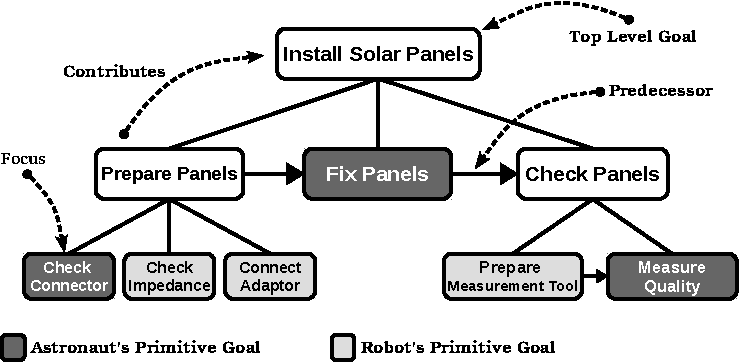
\includegraphics[width=0.97\textwidth]{figure/collaborationStructure-small-croped.pdf}
  \caption{Example of collaboration structure.}
  \label{fig:cs}
  \vspace*{-2mm}
\end{figure}

The Collaboration mechanism constructs a hierarchy of goals associated with
tasks in the form of a hierarchical task network (see Figure \ref{fig:cs}), and
also manages the constraints and other required details of the collaboration
including the inputs and outputs of individual tasks, the \textit{preconditions}
(specifying whether it is appropriate to perform a task), and the
\textit{postconditions} (specifying whether a just-completed task was
successful). Collaboration also keeps track of the focus of attention, which
determines the salient objects, properties and relations at each point, and
shifts the focus of attention during the interaction. For example in Figure
\ref{fig:cs}, ``Check Connector'' is the current (focused) goal\footnote{The
focused goal is the goal that the robot currently pursues.}.

Here, we describe the methods which retrieve information about the collaboration
structure, and are used in our algorithms to compute the values of appraisal
variables. Some of these methods use the \textit{focus stack} which includes a
stack of goals and the top goal on the focus stack represents the current
pursuing goal. In these methods, $\varepsilon_t$ is the event corresponding to
time \textit{t}, and $g_t$ is a given goal at time \textit{t}.

\begin{itemize}
  \setlength\itemsep{1mm}
  \item \textit{getPrimitiveGoal($\varepsilon_t$)} returns the unique primitive
  goal to which the given event (action, utterance, or emotional expression)
  \textit{directly} contributes; it is only one goal since the robot can only do
  one primitive action at a time in our collaboration model, i.e, in the goal
  tree, a given primitive action can only directly contribute to one parent
  goal. The method returns \textsc{ambiguous} if it does not find a goal in
  the plan\footnote{Ambiguity introduces some extra complexities which are
  beyond scope of this thesis.}.
  
  \item \textit{getGoalStatus($g_t$)} returns whether $g_t$'s status is
  \textsc{achieved, failed, blocked, inapplicable, pending,} or
  \textsc{inprogress}.
  
  \item \textit{getTopLevelGoal($g_t$)} returns $g_t$'s top level goal.

  \item \textit{precondStatus($g_t$)} returns the status of the precondition for
  the given goal; whether it is \textsc{satisfied, unsatisfied} or
  \textsc{unknown}. For instance, the precondition for attaching a panel is
  whether the panel is appropriately located on its frame.
  
  \item \textit{isLive($g_t$)} returns \textit{true} iff all the predecessors of
  $g_t$ are \textsc{achieved} and all the preconditions are {\textsc{satisfied}
  &\myeq \textsc{pending} \bigvee \textsc{inprogress}}
  
  \item \textit{isFocusShift($g_t$)} returns \textit{true} iff the given
  goal was not the previous focus (at time t-1).
  
  \item \textit{isNecessaryFocusShift($g_t$)} returns \textit{true} iff the
  status of the previous focus was \textsc{achieved}
  \cite{rich:focused-unfocused-users}.
  
  \item \textit{isPath($g_1$, $g_2$)} returns \textit{true} iff there is a path
  between $g_1$ and $g_2$ in a plan tree structure.
  
%   \item \textit{doesContribute($g_t$)} returns whether the given goal
%   contributes to another goal in the higher level of the plan hierarchy. For
%   instance, an abstract (nonprimitive) goal of ``Bring Panels'' contributes to
%   the higher level goal of ``Install Solar Panels''.
  
  \item \textit{getContributingGoals($g_t$)} returns $g_t$'s children in plan
  tree.
  
  \item \textit{getPredecessors($g_t$)} returns $g_t$'s predecessors in plan
  tree.
  
  \item \textit{getInputs($g_t$)} returns all required inputs for $g_t$. For
  example, the goal ``Attach Panels'' requires the inputs \textit{welding tool}
  and \textit{panel}.
  
  \item \textit{isInputAvailable($g_t$)} returns whether the given input is
  available. For instance, whether the \textit{welding tool} is available for
  the goal ``Attach Panels''.
  
%   \item \textit{isAchieved($g_t$)} returns whether the given goal is achieved,
%   i.e., whether all the postconditions of the given goal are \textsc{satisfied}.
  
  \item \textit{isFocused($g_t$)} returns whether $g_t$ is the current focus.
  
  \item \textit{getResponsible($g_t$)} returns responsible agent(s) for $g_t$.
  In a dyadic collaboration, both of the agents jointly can be responsible for
  a nonprimitive goal, while only one agent (self or other) is responsible for
  each primitive goal. For instance, both the Robot and the Astronaut are
  responsible for the nonprimitive goal of ``Install Solar Panels'', whereas it
  is only the Robot who is responsible for the primitive goal of ``Prepare
  Measurement Tool''.
\end{itemize}

\section{Appraisal Mechanism and Underlying Processes}
\label{sec:appraisal}
In this section, we focus on the specific problem of appraising the
\textit{Relevance} (since other appraisals are only computed for relevant
events), \textit{Desirability} (since it discriminates facilitating and
inhibitory events towards the collaboration progress), \textit{Expectedness}
(since it underlies a collaborative robot's attention), and
\textit{Controllability} (since it is associated with the agent's coping
ability) of events within a collaborative interaction. There are other appraisal
variables introduced in psychological \cite{scherer:appraisal-processes} and
computational literature \cite{gratch:domain-independent}. We believe most of
these variables can be straightforwardly added to our appraisal mechanism
whenever they are required. All of the algorithms in this section use the mental
state of the robot (discussed in Section \ref{sec:mental-states}) which is
formed based on the collaboration structure (see Figure
\ref{fig:appraisal-collaboration}). These algorithms use the corresponding
primitive goal to the most recent event at each turn.

\begin{figure}[tbh]
  \centering
  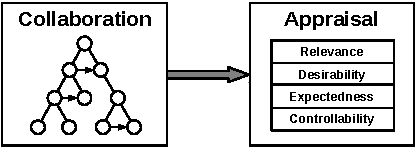
\includegraphics[width=0.8\textwidth]{figure/appraisal-collaboration-croped.pdf}
  \caption{Using Collaboration structure in Appraisal (mechanisms in our
  framework).}
  \label{fig:appraisal-collaboration}
\end{figure}

\subsection{Relevance}
\label{sec:relevance}
Relevance is a key appraisal variable since the other appraisal variables
are meaningful only for relevant events. Relevance as an appraisal variable
measures the significance of an event for the self. An event can be evaluated to
be relevant if it has a non-zero utility \cite{marsella:ema-process-model}.
However, the utility of an event is also influenced by the other collaborator's
emotional expressions as the reflection of the other collaborator's mental state
with respect to the status of the collaborative environment. Other appraisal
models only consider the utility of an event based on the self's goal and plan.

Algorithm \ref{alg:relevance} determines the relevance of the given event with
respect to the current mental state. The relevance of the event depends on the
significance of the event with respect to the collaboration status, which is
determined based on the utility of the event as presented in
\cite{gratch:domain-independent,marsella:ema-process-model}. Our algorithm for
computing the relevance of an event during collaboration involves other factors
that other appraisal models do not consider. For instance, the human's
perceived emotion, recurrence of a belief, or occurrence of a belief about an
unrelated goal by the human play important roles by influencing the utility
of an event during collaboration. As a result, evaluating the relevance of
events can cause a collaborative robot to respond effectively which can
positively impact the status of the shared goal, without dedicating all its
resources to every event.

After perceiving an event, the belief about that event represents the event in
the robot's mental state. \textit{getPrimitiveGoal} returns the goal to which
the current event contributes, unless it is \textsc{ambiguous}; $g_{t}$
represents the shared goal at time (turn) $t$ within the shared plan. 

\vspace*{-4mm}
\subsubsection{Utility of an Event}
We compute the utility ($-1 \leq \mathcal{U} \leq 1$) of the event using the
values of the attributes associated with the existing beliefs, and the
attributes of the motive associated with the recognized goal (see details
below). We use three belief attributes (i.e., \textit{Strength, Saliency,} and 
\textit{Persistence} -- see Section \ref{sec:mental-states}) to compute the
belief-related part of the utility:

\begin{algorithm}
	\caption{(Relevance)}
	\label{alg:relevance}
	\begin{algorithmic}[1]
		\Function{IsEventRelevant}{Event $\varepsilon_t$}
 			\Statex
			\State $\mathit{g}_{t} \gets \textit{getPrimitiveGoal}{(\varepsilon_t)}$
 			\Statex
			\State $\mathcal{U} \gets \Call{getEventUtility}{\mathit{g}_{t}}$
			\State $\tau_{t} \gets \Call{getEmotionalThreshold}{\mathit{g}_{t}}$
 			\Statex
			\If {$(\tau_{t} \leq |\mathcal{U}|)$}  
 				\State \Return {{\fontsize{7}{8}\selectfont RELEVANT}}
			\Else 
 				\State \Return {{\fontsize{7}{8}\selectfont IRRELEVANT}}
			\EndIf
		\EndFunction
	\end{algorithmic}
\end{algorithm}

We provide the utility function ($\mathcal{U}$) in Equation \ref{eqn:utility}.
This function uses: saliency (\textit{S}) and persistence (\textit{P}) of the
belief related to the recognized goal, the recognized goal's status
($\upsilon$), and the aggregation of belief and motive attributes ($\Psi$)
according to Equation \ref{eqn:utility}.

\begin{equation}
    \mathcal{U}(g_t)= 
    \begin{dcases}
       \upsilon\!P\cdot S^{\Psi} & \Psi \textgreater 0 \\
       0               			 & \Psi = 0
    \end{dcases}
    \label{eqn:utility}
\end{equation}

Intuitively, we use $\upsilon$ to generate positive and negative utility values.
The $\upsilon$'s value becomes +1 if the status of the corresponding goal is
\textsc{achieved}, \textsc{pending}, or \textsc{in progress}, and $\upsilon$'s
value becomes -1 if the status of the corresponding goal is \textsc{failed,
blocked}, or \textsc{inapplicable}. The \textit{P} influences the value of
utility only as a coefficient since recurrent beliefs are not formed frequently
during collaboration. The $\Psi$ value indicates the magnitude of the influence
of beliefs and motives using their attributes. Hence, the $\Psi$ value impacts
the saliency value of beliefs exponentially, helping to differentiate between
beliefs.

\begin{itemize}
  \setlength\itemsep{1mm}
  \item \textit{Strength}: The extent to which the preconditions ($\alpha$),
  postconditions ($\beta$), predecessors ($\lambda$), and contributing goals
  ($\mu$) of a goal are known (\textsc{satisfied} or \textsc{unsatisfied}) makes
  beliefs about the goal stronger. An \textsc{unknown} pre and postcondition
  status of a goal and its predecessors and contributing goals forms weaker
  beliefs. For instance, if one knows all predecessors of a pursued goal (e.g.,
  ``Check Panels'') are \textsc{satisfied} (i.e., ``Fix Panels'' and ``Prepare
  Panels''), failure of the pursued goal will elicit one's negative emotion (due
  to the strong beliefs related to the goal); whereas not knowing the status of
  the goal-related factors (e.g., whether the Astronaut could find the tool to
  fix a panel) causes one to form weaker beliefs about the goal.
\end{itemize}
In equation \ref{eqn:exponent}, the subscript \textit{k} refers to the
\textit{known} goal-related factors (\textsc{satisfied} or
\textsc{unsatisfied}); whereas the subscript \textit{all} includes both
\textit{known} and \textit{unknown} goal-related factors. In this equation, both
urgency ($\gamma$) and importance ($\eta$) attributes of motives can impact the
outcome of the goal-related belief attributes' ratio, and ultimately the $\Psi$
value.

\begin{equation}
    \Psi = \frac{\alpha_{_k} + \beta_{_k} + \lambda_{_k} +
    \mu_{_k}}{\alpha_{_{all}} + \beta_{_{all}} + \lambda_{_{all}} +
    \mu_{_{all}}} + \eta + \gamma
    \label{eqn:exponent}
\end{equation}

\begin{center} 
    $\eta, \gamma \in \mathbb{N}, \qquad\qquad \eta, \gamma \geq 0$\\
    $\alpha_{_k}, \beta_{_k}, \lambda_{_k}, \mu_{_k} \in \mathbb{N},
    \qquad\qquad \alpha_{_k}, \beta_{_k}, \lambda_{_k}, \mu_{_k} \geq 0$\\
    $\alpha_{_{all}}, \lambda_{_{all}}, \mu_{_{all}} \in \mathbb{N},
    \qquad\qquad \alpha_{_{all}}, \lambda_{_{all}}, \mu_{_{all}} \geq 0$\\
    $\beta_{_{all}} \in \mathbb{N}, \qquad\qquad \beta_{_{all}} \geq 1$
\end{center}

\begin{itemize}
  \setlength\itemsep{1mm}
  \item \textit{Saliency (S)}: Beliefs related to the focused goal are more
  salient than beliefs related to any other goal in the plan; according to
  Figure \ref{fig:cs}, if one of the collaborators is preparing a solar panel,
  beliefs related to all of the other \textit{live} (\textsc{pending} or
  \textsc{in progress}) goals (e.g. ``Connect Adaptor'') will be less salient
  than beliefs related to the focused goal, i.e., ``Check Connector''. Beliefs'
  saliency decreases according to their corresponding \textit{live} goal's
  distance from the focused goal in the shared plan. \textit{Non-live} goals
  will not be salient.
  \item \textit{Persistence (P)}: The recurrence of a belief over time (turns)
  increases the persistence of the belief. Beliefs occurring only once have the
  lowest value of persistence. For instance, if the Astronaut repeatedly says
  that she can not find the measurement tool to check the connector, the Robot
  could pursue a new goal outside of the shared plan to acknowledge Astronaut's
  concern.
\end{itemize}

\noindent We also use two motive attributes discussed in Section
\ref{sec:mental-states} to compute the motive related part of the utility
($\mathcal{U}$):

\begin{itemize}
  \setlength\itemsep{1mm}
  \item \textit{Urgency ($\gamma$)}: There are two factors impacting the urgency
  of a motive: a) whether the goal directing the given motive is the predecessor of
  another goal for which the other collaborator is responsible, and b) whether
  achieving the goal directing the given motive can mitigate the other
  collaborator's negative valenced emotion. For instance, if the Robot has a
  private goal to fetch another panel while the Astronaut is waiting for the
  Robot to connect the adaptor, connecting the adaptor will be more urgent than
  Robot's private goal.
  \item \textit{Importance ($\eta$)}: A motive is important if failure of the
  directing goal causes an impasse in the shared plan (i.e., no further goal is
  available to achieve), or achievement of the directing goal removes an
  existing impasse. For example, if the Robot cannot find the adaptor (an
  impasse to connect the adaptor), and the Astronaut provides another adaptor
  (external motive), the new motive becomes important to remove the impasse in
  the shared plan.
\end{itemize}

The significance of an event in a collaborative environment is based on the
utility of the event and the human's perceived emotion. The human's perceived
emotion influences the relevance of the event in the form of a threshold value
$\tau_{t}$ in Algorithm \ref{alg:relevance}. In Equation \ref{eqn:threshold}, we
use the valence of the perceived emotion ($\mathcal{V}_{e_h}$) to compute
$\tau_{t}$.

\begin{equation}
    \tau_{t}= 
    \begin{dcases}
       1-\mathcal{V}_{e_h} & \mathcal{V}_{e_h} > 0 \\
       |\mathcal{V}_{e_h}| & \mathcal{V}_{e_h} \leq  0
    \end{dcases}
    \label{eqn:threshold}
\end{equation}

\begin{center} 
    $\mathcal{V}_{e_h} \in \mathbb{R}, \qquad\qquad -1 \leq \mathcal{V}_{e_h}
    \leq 1$
\end{center}

Hence, perceiving human's positive emotion (e.g., happiness) reduces the
threshold value which makes the robot find an event \textsc{relevant} with even
a slightly positive utility. Similarly, an event can be considered
\textsc{irrelevant} even though the utility has a relatively positive value,
because of perceiving the human's negative emotion.

\subsection{Desirability}
Desirability characterizes the value of an event to the robot in terms of
whether the event facilitates or thwarts the collaboration goal. Desirability
captures the valence of an event with respect to the robot's preferences
\cite{gratch:domain-independent}. In a collaborative robot, preferences are
biased towards those events facilitating progress in the collaboration.
Desirability plays an important role in the overall architecture; it makes the
processes involved in the other mechanisms (e.g., Motivation and Theory of
Mind) and consequently the robot's mental state, congruent with the
collaboration status which is a collaborative robot's desire. Therefore, it
causes the robot to dismiss events causing inconsistencies in the robot's
collaborative behavior. Moreover, desirability is also crucial from the
collaboration's point of view.

% A collaborative robot needs to know whether its own and the other collaborator's
% actions, utterances, and emotional expressions are desirable in terms of their
% consistence with the status of the current shared goal. In other words, the
% collaboration mechanism uses the appraisal process of desirability to coordinate
% what the self or the other does, says, and expresses during collaboration.
% Reciprocally, the appraisal mechanism and in this case the desirability process
% use the collaboration structure to obtain their required information.

\begin{algorithm}[tbh]
	\caption{(Desirability)}
	\label{alg:desirability}
	\begin{algorithmic}[1]
		\Function{IsEventDesirable}{Event $\varepsilon_t$}
			\Statex
			\State $\mathit{g}_{t} \gets \textit{getPrimitiveGoal}{(\varepsilon_t)}$
			\State $\mathit{g}_{top} \gets \textit{getTopLevelGoal}{(\mathit{g}_{t})}$
			\Statex
			\If {(\textit{getGoalStatus($g_{top}$)} =
			{\fontsize{8}{9}\selectfont ACHIEVED})}
			\State \Return {{\fontsize{8}{9}\selectfont MOST-DESIRABLE}} 
			\ElsIf {(\textit{getGoalStatus($g_{top}$)} =
			{\fontsize{8}{9}\selectfont FAILED})} 
			\State \Return {{\fontsize{8}{9}\selectfont MOST-UNDESIRABLE}}
			\ElsIf {(\textit{getGoalStatus($g_{top}$)} =
			{\fontsize{8}{9}\selectfont BLOCKED}) \OR\\
			\hspace*{19.5mm}(\textit{getGoalStatus($g_{top}$)} =
			{\fontsize{8}{9}\selectfont INAPPLICABLE})}
			\State \Return {{\fontsize{8}{9}\selectfont UNDESIRABLE}} 
			\ElsIf {(\textit{getGoalStatus($g_{top}$)} =
			{\fontsize{8}{9}\selectfont PENDING}) \OR\\
			\hspace*{19.5mm}(\textit{getGoalStatus($g_{top}$)} =
			{\fontsize{8}{9}\selectfont INPROGRESS})}
				\Statex
				\If {(\textit{getGoalStatus($g_{t}$)} =
				{\fontsize{8}{9}\selectfont ACHIEVED})}
				\State \Return {{\fontsize{8}{9}\selectfont DESIRABLE}}
				\ElsIf {(\textit{getGoalStatus($g_{t}$)} = {\fontsize{8}{9}\selectfont
				FAILED})} 
				\State \Return {{\fontsize{8}{9}\selectfont MOST-UNDESIRABLE}}
				\ElsIf {(\textit{getGoalStatus($g_{t}$)} = {\fontsize{8}{9}\selectfont
				BLOCKED}) \OR \\
				\hspace*{25.5mm}(\textit{getGoalStatus($g_{t}$)} =
				{\fontsize{8}{9}\selectfont INAPPLICABLE})} 
				\State \Return {{\fontsize{8}{9}\selectfont UNDESIRABLE}}
				\ElsIf {(\textit{getGoalStatus($g_{t}$)} =
				{\fontsize{8}{9}\selectfont PENDING}) \OR \\ \hspace{1mm} 
				\hspace*{23.5mm}(\textit{getGoalStatus($g_{t}$)} =
				{\fontsize{8}{9}\selectfont INPROGRESS})} 
				\State \Return {{\fontsize{8}{9}\selectfont NEUTRAL}}
				\EndIf
			\EndIf
		\EndFunction
	\end{algorithmic}
\end{algorithm}

Algorithm \ref{alg:desirability} defines a process in which the desirability of
an event is computed with regard to the status of the shared goal; i.e., it
operates based on whether and how the event changes the status of the current
shared goal. It distinguishes between the top level goal and the current goal
because the top level goal's change of status attains a higher positive or
negative value of desirability. For instance, failure of the top level goal
(e.g., installing solar panel) is more undesirable than failure of a primitive
goal (e.g., measuring the quality of the installed panel).

% An \textsc{ambiguous} goal is a goal associated with the current event
% ($\varepsilon_t$) which is not recognized in the robot's plan; therefore it is
% \textsc{undesirable} for a collaborative robot. 

A top level goal's status must be \textsc{achieved} (i.e., \textsc{satisfied}
postcondition) to consider the event \textsc{most-desirable}. When the goal's
status is \textsc{failed} (i.e., \textsc{unsatisfied} postcondition) or
\textsc{blocked}, the associated event has the \textsc{most-undesirable} or
\textsc{undesirable} values respectively. A goal is \textsc{blocked} if any of
the required goals or goals recursively through the parent goal are not
\textsc{achieved}. An \textsc{inapplicable} goal is also considered as
\textsc{undesirable}. A goal is \textsc{inapplicable} if any of its predecessors
are not \textsc{achieved}, and/or its preconditions are not \textsc{satisfied}.
For \textsc{pending} and \textsc{inprogress} top level goals, the status of the
current goal associated with the top level goal determines the status of the
event $\varepsilon_t$. Only a non-primitive goal can have \textsc{inprogress}
status, if it has been started but is not yet completed. A goal can be
\textsc{pending} if it is live, or if it is a non-primitive goal that has not
been started yet. \textsc{Achieved} current goals mark an event
($\varepsilon_t$) as \textsc{desirable}, while \textsc{failed} or
\textsc{blocked} current goals render the event associated with them as
\textsc{most-undesirable} and \textsc{undesirable} respectively.
\textsc{Pending} or \textsc{inprogress} current goals mark their associated
events as \textsc{neutral}.

\subsection{Expectedness}
Expectedness is the extent to which the truth value of a state could have been
predicted from a causal interpretation of an event. In the collaboration
context, the expectedness of an event evaluates the congruency of the event with
respect to the existing knowledge about the shared goal. Thus, expectedness
underlies a collaborative robot's attention. The collaboration mechanism uses
expectedness to maintain the robot's attention and subsequently its mental state
with respect to the shared goal. Reciprocally, the appraisal mechanism uses the
underlying information of the collaboration structure to evaluate the
expectedness of an event \cite{shayganfar:appraisal-short}.

\begin{algorithm}
	\caption{(Expectedness)}
	\label{alg:expectedness}
	\begin{algorithmic}[1]
		\Function{IsEventExpected}{Event $\varepsilon_t$}
			\Statex
			\State $\mathit{g}_{t} \gets \textit{getPrimitiveGoal}{(\varepsilon_t)}$
			\State $\mathit{g}_{top} \gets \textit{getTopLevelGoal}{(\mathit{g}_{t})}$
			\Statex
			\If {$(\textit{isLive}{(\mathit{g}_{t})})$}
				\If {$(\neg \textit{isFocusShift}{(\mathit{g}_{t})}\hspace*{2mm}\OR$ 
				$\textit{isNeccessaryFocusShift}{(\mathit{g}_{t})})$}
				\State \Return {\fontsize{7}{8}\selectfont MOST-EXPECTED}
				\Else
					\State \Return {\fontsize{7}{8}\selectfont EXPECTED}
				\EndIf
			\Else
				\If {$(\textit{isPath}{(\mathit{g}_{t}, \mathit{g}_{top})})$}
					\State \Return {\fontsize{7}{8}\selectfont UNEXPECTED}
				\Else
					\State \Return {\fontsize{7}{8}\selectfont MOST-UNEXPECTED}
				\EndIf
			\EndIf
		\EndFunction
	\end{algorithmic}
\end{algorithm}

In Algorithm \ref{alg:expectedness} we define the process of computing the
expectedness based on the shared plan and status of the shared goal. The key
point in this algorithm is the status of the current shared primitive goal
($\mathit{g}_{t}$), which is associated with the event $\varepsilon_t$ and its
relationship with the top level goal ($\mathit{g}_{_{top}}$).

The intuition captured here is that one expects the current goal to be finished
before undertaking another activity, but the goals that can be the next focus of
attention are also to be expected. Therefore, if the goal is live, the algorithm
checks whether the goal has not changed, or whether the interpretation of the
last event results in a necessary focus shift. Shifting the focus to a new goal
is necessary when the former goal is achieved and a new goal is required.
Consequently the new event is the \textsc{most-expected} one. However, even if
the focus shift is not necessary, the new event can be considered as
\textsc{expected}, since the corresponding goal is already live. For goals that
have not yet been started (that is, are not live), the algorithm must determine
how unexpected it would be to pursue one now; if the goal is at least in the
plan, i.e., on the path to the top level goal, it is just \textsc{unexpected}
while any others are \textsc{most-unexpected}.

\subsection{Controllability}
\label{sec:controllability}
Controllability is the extent to which an event can be influenced; it is
associated with a robot's ability to cope with an event
\cite{gratch:domain-independent}. Thus, a robot can determine whether an event's
outcome can be altered by actions under either of the collaborators' control. In
other words, controllability is a measure of a robot's ability to maintain or
change a particular state as a consequence of an event.

\begin{algorithm}
	\caption{(Controllability)}
	\label{alg:controllability}
	\begin{algorithmic}[1]
		\Function{IsEventControllable}{Event $\varepsilon_t$}
 			\State $\mathit{g}_{t} \gets \textit{getPrimitiveGoal}{(\varepsilon_t)}$
  			\Statex
			\State $\mathcal{M} \gets \Call{GetAgencyRatio}{\mathit{g}_{t}}$ 
			\State $\mathcal{R} \gets \Call{GetAutonomyRatio}{\mathit{g}_{t}}$
 			\Statex
			\State $\mathcal{P} \gets \Call{GetSuccPredecessorsRatio}{\mathit{g}_{t}}$
			\State $\mathcal{I} \gets \Call{GetAvailableInputs}{\mathit{g}_{t}}$
  			\Statex
			\State $\mathcal{V}_{e_h} \gets \Call{getEmotionValence}{\mathit{g}_{t}}$ 
			\State $\omega \gets \Call{getWeights}{\mathit{g}_{t}}$
			\Statex
			\State $\mathcal{X} \gets
			\frac{\omega_{0}\cdot \mathcal{M} + \omega_{1}\cdot \mathcal{R} +
			\omega_{2}\cdot \mathcal{P} + \omega_{3}\cdot \mathcal{I}}{\omega_{0} +
			\omega_{1} + \omega_{2} + \omega_{3}} + \mathcal{V}_{e_h}$
  			\Statex
% 			\State $\tau_{t} \gets \Call{getEmotionalThreshold}{\mathit{g}_{t}}$
 			\Statex
			\If {$(\mathcal{X} > 0)$}
 				\State \Return {{\fontsize{7}{8}\selectfont CONTROLLABLE}}
			\Else 
 				\State \Return {{\fontsize{7}{8}\selectfont UNCONTROLLABLE}}
			\EndIf
		\EndFunction
	\end{algorithmic}
\end{algorithm}

Controllability is important for the overall architecture. For instance, the
robot can choose to ask or negotiate about a collaborative task which is not
controllable, or form a new motive to establish an alternative goal for the
current uncontrollable event. In general, other mechanisms in the architecture
use the controllability output in their decision-making processes; while
controllability uses information from the collaboration structure, e.g.,
predecessors of a goal.

An important determinant of one's emotional response is the sense of control
over occurring events. This sense of subjective control is based on one's
reasoning about the self's power. For instance, the robustness of one's plan for
executing actions can increase one's sense of power and subsequently the sense
of control. In the collaboration context, we have translated the sense of control
into a combination of four different factors including a) \textit{agency} and b)
\textit{autonomy} of the robot, as well as the ratios of c) \textit{successful
predecessors}, and d) the \textit{available inputs} of a given goal
(i.e., $\mathit{g}_{t}$) in the shared plan.

In Algorithm \ref{alg:controllability}, we partially compute the controllability
of an event based on the above four factors. We use weighted averaging of these
factors to determine their impact on the controllability of an event (line 9).
The value of all these weights are set to \textit{1.0} for the purpose of
simplicity (\textbf{$\Call{getWeights}{}$}). These weights can be adjusted after
further investigating the influence of these factors, and implementing other
mechanisms in the overall architecture. We believe that the human's perceived
emotion also impacts the controllability of an event
(\textbf{$\Call{getEmotionValence}{}$}). The ($-1.0 \leq \mathcal{V}_{e_h} \leq
1.0$) is the valence value of the human's perceived emotion. Positive emotions,
e.g., happiness, possess positive values, and negative emotions, e.g., anger,
have negative values. The magnitude of this value can change with respect to the
intensity of the perceived emotion. Thus, a positive controllability value
indicates that an event is \textsc{controllable}; otherwise
\textsc{uncontrollable}.

% \renewcommand\thealgorithm{4\alph{algorithm}}
% \setcounter{algorithm}{0}
% 
% \begin{algorithm}
% 	\caption{(Get Agency Ratio)}
% 	\label{alg:agency}
% 	\begin{algorithmic}[1]
% 		\Function{GetAgencyRatio}{Event $\varepsilon_t$}
% 			\Statex
% 			\State $\mathit{g}_{t} \gets \textit{recognizeGoal}{(\varepsilon_t)}$
% 			\Statex
% 			\State $\mathcal{M}_{t} \gets \textit{getActiveMotive}{(\mathit{g}_{t})}$
% 			\Statex
% 			\If {$(\mathcal{M}_{t} \neq \emptyset)$}
% 				\If {$(\mathcal{M}_{t}\cdot type = $
% 				{{\fontsize{8}{8}\selectfont INTERNAL}}$)$} \State \Return {1.0}
% 				\Else
% 					\State \Return {0.0}
% 				\EndIf
% 			\Else
% 				\State \Return {0.0}
% 			\EndIf
% 		\EndFunction 
% 	\end{algorithmic}
% \end{algorithm}

$\Call{\textbf{GetAgencyRatio}}{}$: \textit{Agency} is the capacity of an
individual to act independently in a given environment. In a collaborative
environment collaborators are sometimes required to act independently of each
other. Hence, they need to have some internal motives that are formed based on
their own mental states rather than motives that are reinforced by the other.
These internal motives will lead the collaborators to acquire new intentions
when required. If the robot's mental state possesses only an internal motive
supporting the recognized goal, we consider a maximum agency value denoted as
$\mathcal{M}$ in Algorithm \ref{alg:controllability} (i.e., $\mathcal{M}=1.0$);
otherwise we consider the minimum agency value (i.e., $\mathcal{M}=0.0$). 

% \renewcommand\thealgorithm{4\alph{algorithm}}
% \setcounter{algorithm}{1}
% 
% \begin{algorithm}
% 	\caption{(Get Autonomy Ratio)}
% 	\label{alg:autonomy}
% 	\begin{algorithmic}[1]
% 		\Function{GetAutonomyRatio}{Event $\varepsilon_t$}
% 			\Statex
% 			\State $\mathit{g}_{t} \gets \textit{recognizeGoal}{(\varepsilon_t)}$
% 			\Statex
% 			\State $\Phi_{\mathit{g}} \gets
% 			\textit{extractContributingGoals}{(\mathit{g}_{t})}$
% 			\Statex
% 			\ForAll {$\phi_{\mathit{g}}^i \in \Phi_{\mathit{g}}$}
% 				\If {$(\textit{getResponsible}{(\phi_{\mathit{g}}^i)} =$
% 				{\fontsize{8}{8}\selectfont SELF})} 
% 					\State $count_{self} \gets count_{self} + 1$
% 				\EndIf
% 			\EndFor
% 			\Statex
% 			\State \Return 
% 			${count_{self} \mathbin{/} {{\Phi_{\mathit{g}}}.total()}}$
% 		\EndFunction 
% 	\end{algorithmic}
% \end{algorithm}

$\Call{\textbf{GetAutonomyRatio}}{}$: \textit{Autonomy} is the ability to make
decisions without the influence of others, and implies acting on one's own and
being responsible for that. In a collaborative environment, tasks are delegated
to the collaborators based on their capabilities. Therefore, each collaborator
is responsible for the delegated task and the corresponding goal. In Algorithm
\ref{alg:controllability}, $\mathcal{R}$ denotes the value of autonomy with
regard to the goal $\mathit{g}_{t}$. This value $(0.0 \leq \mathcal{R} \leq
1.0)$ is the ratio of the number of goals contributing to $\mathit{g}_{t}$ for
which the robot is responsible over the total number of contributing goals, if
the goal associated with the current event is a nonprimitive goal. However, if
the associated goal of the current event corresponds to a primitive goal the
value of $\mathcal{R}$ would be 0.0 (if the human is responsible) or 1.0 (if the
robot is responsible). In general, higher autonomy leads to a more positive
value of controllability.

% \renewcommand\thealgorithm{4\alph{algorithm}}
% \setcounter{algorithm}{2}
% 
% \begin{algorithm}
% 	\caption{(Get Successful Predecessors Ratio)}
% 	\label{alg:predecessors}
% 	\begin{algorithmic}[1]
% 		\Function{GetSucPredecessorsRatio}{Event $\varepsilon_t$}
% 			\Statex
% 			\State $\mathit{g}_{t} \gets \textit{recognizeGoal}{(\varepsilon_t)}$
% 			\Statex
% 			\State $\Theta{\mathit{g}} \gets
% 			\textit{extractPredecessors}{(\mathit{g}_{t})}$
% 			\Statex
% 			\ForAll {$\theta_{\mathit{g}}^i \in \Theta_{\mathit{g}}$}
% 				\If {$(\textit{isAchieved}{(\theta_{\mathit{g}}^i)})$}
% 					\State $count_{achieved} \gets count_{achieved} + 1$
% 				\EndIf
% 			\EndFor
% 			\Statex
% 			\State \Return
% 			${count_{achieved} \mathbin{/} {\Theta{\mathit{g}}.total()}}$
% 		\EndFunction 
% 	\end{algorithmic}
% \end{algorithm}

$\Call{\textbf{GetSuccPredecessorsRatio}}{}$: The structure of a shared plan
contains the order of the required \textit{predecessors} of a goal. Predecessors
of a goal, $g_t$, are goals that the collaborators should achieve before trying
to achieve goal $g_t$. We use the ratio of successfully achieved predecessors of
the associated primitive goal over the total number of predecessors of the same
goal. If all of the predecessors of the given goal are achieved, then
$\mathcal{P}=1.0$ which is the maximum value for $\mathcal{P}$. On the contrary,
failure of all of the predecessors will lead to $\mathcal{P}=0.0$. Therefore, a
higher $\mathcal{P}$ value positively impacts the value of controllability for
the current event.

% \renewcommand\thealgorithm{4\alph{algorithm}}
% \setcounter{algorithm}{3}
% 
% \begin{algorithm}
% 	\caption{(Get Available Input Ratio)}
% 	\label{alg:inputs}
% 	\begin{algorithmic}[1]
% 		\Function{GetAvailableInputRatio}{Event $\varepsilon_t$}
% 			\Statex
% 			\State $\mathit{g}_{t} \gets \textit{recognizeGoal}{(\varepsilon_t)}$
% 			\Statex
% 			\State $\mathcal{X}_{\mathit{g}} \gets
% 			\textit{extractInputs}{(\mathit{g}_{t})}$
% 			\Statex
% 			\ForAll {$\chi_{\mathit{g}}^i \in \mathcal{X}_{\mathit{g}}$}
% 				\If {$(\textit{IsAvailable}{(\chi_{\mathit{g}}^i)})$}
% 					\State $count_{available} \gets count_{available} + 1$
% 				\EndIf
% 			\EndFor
% 			\Statex
% 			\State \Return
% 			${count_{available} \mathbin{/} \mathcal{X}_{\mathit{g}}.total()}$
% 		\EndFunction 
% 	\end{algorithmic}
% \end{algorithm}

$\Call{\textbf{GetAvailableInputs}}{}$: Finally, \textit{inputs} of a task are
the required elements that the collaborators use to achieve the specified goal
of the task. These inputs are also part of the structure of a shared plan. We
compute the ratio of the available required inputs over the total required
inputs of the goal associated with the current event. This value (denoted as
$\mathcal{I}$ in Algorithm \ref{alg:controllability}) will be set between 0.0
and 1.0. Similar to the other factors in the controllability process, the closer
the value of $\mathcal{I}$ gets to 1.0, the more positive impact it has on the
overall controllability value of the event.\\

In summary, the output of these four appraisal processes serves as critical
input for the other mechanisms of the Affective Motivational Collaboration
framework, shown in Chapter \ref{ch:amct}. By providing adequate interpretation
of events in the collaborative environment, the appraisal mechanism enables the
robot to carry out proper collaborative behaviors.

\section{Goal Management}
\label{sec:goal-management}

A collaborative robot needs to be able to regulate and manage shared goals
during collaboration. Emotion has a crucial influence on this goal management
process. In this section, we provide a cost function that we use to choose the
goal in the shared plan with the lowest cost value out of a set of alternative
goals. This cost function is a) based on the goal attributes, b) with respect to
the reverse appraisal of the perceived emotion, and c) the appraisal of the
collaborative environment. Adding goal management process to Collaboration
mechanism is one of our contributions.

Goals represent a key part of the context during collaboration. However, not all
goals are appropriate to pursue at the moment, depending on conditions. In fact,
it can be destructive for a collaboration to pursue a plausible goal in a poor
context. Therefore, a collaborative robot must be able to manage shared goals
during collaboration. The goal management process has a critical influence on a
collaborative robot's behavior by maintaining or shifting the focus of attention
to an appropriate goal based on the collaboration status.

Changes in a collaboration environment alter the relative importance of
alternative goals. These changes can reflect the collaborators' internal changes
and the influence of their actions. In a collaboration environment, emotions
represent the outcome of underlying mental processes of the collaborators.
Emotions have many different functions
\cite{scheutz:architectural-action-selection} including goal management.
Goal-oriented emotions such as anger, frustration and worry regulate the mental
processes influenced by one's internal goals. In our ongoing example, a robot
and an astronaut are collaborating to install solar panels. When one of the
astronaut's goals is blocked, the robot must manage the shared goals in order to
prevent failure of the collaboration. By using reverse appraisal
\cite{gratch:reverse-appraisal} of the astronaut's emotion and its own appraisal
of individual goals, the robot is able to successfully shift the focus of
attention from the blocked goal (eliciting worry in the astronaut) to an
appropriate one to maintain the collaboration. A similar example is provided in
Chapter \ref{ch:awareness}.

\begin{figure}[t]
  \centering
  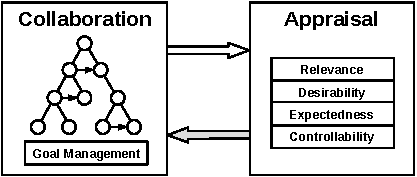
\includegraphics[width=0.8\textwidth]{figure/goal_management_croped.pdf}
  \caption{Using Appraisals' outcome to influence Collaboration structure
  (mechanisms in our framework).}
  \label{fig:appraisal-on-collaboration}
\end{figure}

Here, we describe the goal management process in our framework using an
astronaut-robot collaboration example. We introduce the goal management process
based on a cost function including the influence of affective appraisal and
reverse appraisal processes. Goal management is a crucial part of our
investigation of the reciprocal influence of appraisal on a collaboration
structure (see Figure \ref{fig:appraisal-on-collaboration}).

As we mentioned earlier, we use four appraisal variables including: relevance,
desirability, expectedness and controllability. The outcome of each appraisal
process is a specific value for the corresponding appraisal variable. The vector
containing these appraisal variables can be mapped to a particular emotion
instance at each point in time when required (see Algorithms in Section
\ref{sec:appraisal}). Moreover, the functions of emotions, such as goal
management, in a social setting and the meaning of the collaborator's perceived
emotion in collaboration context are also important.

A collaboration structure provides a hierarchy and constraints of the shared
goals in the form of a shared plan which contains both the robot and the human
collaborator's goals. The robot pursues the goals for which the robot is
responsible in the shared plan. However, there can be several live goals
available for the robot to pursue at each point in time during collaboration. A
goal is live \textit{iff} all of its predecessors are achieved and all of its
preconditions are satisfied. Therefore, a collaborative robot requires a
mechanism to choose between a set of live goals. We believe appraisal processes
are crucial to choose between the available live goals, since the appraisals are
the immediate outcome of the robot's assessment of the collaboration environment.

\begin{figure}[tbh]
  \centering
  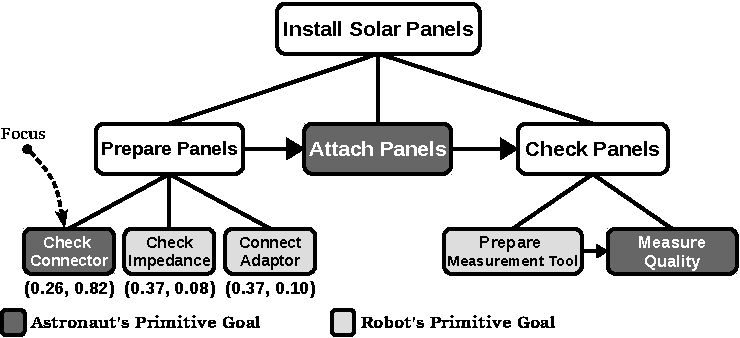
\includegraphics[width=1\textwidth]{figure/goal_management_collaboration_structure-croped.pdf}
  \caption{Cost values indicated by tuples with (second number) and without
  (first number) the influence of emotions.}
  \label{fig:task-model-astronaut}
\end{figure}

For instance, Figure \ref{fig:task-model-astronaut} shows a non-primitive
``Prepare Panels'' goal decomposed into three unordered primitive goals.
Therefore, if ``Prepare Panels'' is live, its primitive goals can be pursued by
the responsible agent. In our example, the astronaut is responsible for the
``Check Connector'' goal; the robot is responsible for the remaining two
primitive goals. According to the collaboration mechanism in our overall
framework, ``Check Connector'' is in focus, with the astronaut pursuing this
goal. Suddenly, however the astronaut tells the robot that she can not find the
connector and she is \textit{worried} about failure of this goal. The robot's
response to this situation will be explored below as we discuss details of our
cost function.

Equation \ref{eqn:cost} shows the function to calculate the cost of each live
goal. Goal management algorithm chooses the minimum cost goal. The base in the
equation calculates the cost of pursuing any given goal. The three functions
used to calculate the cost are: \textit{proximity} $P(g)$, \textit{difficulty}
$D(g)$, and \textit{specificity} $S(g)$ (see equations \ref{eqn:proximity} to
\ref{eqn:specificity}).

\begin{equation}
{\fontsize{6}{9}\selectfont Cost(g) =
\big(\omega_0.P(g)+\omega_1.D(g)+\omega_2.\frac{1}{S(g)+1}\big)}^{\Gamma}
\label{eqn:cost}
\end{equation}

\noindent For simplicity in this example, we assume equal values for the
weights:
$\omega_i$=1.

\begin{equation}
\Gamma=-C[(R_r+1)D_r + \alpha(R_h+1)D_h]
\label{eqn:power}
\end{equation}

The exponent part of our cost function (Equation \ref{eqn:power}) captures a)
the influence of the human's perceived emotional instance, and b) the influence
of self appraisal of the given goal. $R_h\in[0,1]$ and $D_h\in[-1,1]$ are the
relevance and desirability values respectively, which are based on the
\textit{reverse} appraisal of the human's perceived emotion. For instance, if
the astronaut is \textit{worried}, $D_h$ is negative, e.g., -0.8 (depending on
how undesirable the event is according to reverse appraisal), and $R_h$ will be
1 for the active goal and its value descends to 0 for other live goals depending
on their distance to the active goal in the shared plan (e.g., 0.1).

$R_r\in[0,1]$ and $D_r\in[-1,1]$ are relevance and desirability values, provided
by the \textit{self} appraisal functions for all of the live goals. For
instance, for the active goal for which the astronaut was \textit{worried},
$D_r$ can be positive, e.g., 0.8 (depending on the self's desirability appraisal
function); $R_r$ can be 1, since the active goal is relevant for the robot.
These values will change for the other live goals depending on how
relevant they are with respect to the collaboration status (e.g., 0.9 and 0.8).
Finally, $C\in[1,\infty)$ is a constant (e.g., 2) used to control the influence
of affect on cost value. It is negative since undesirability (negative values)
should increase the cost. $\alpha\in[1,\infty)$ is another constant (e.g., 3)
used to control the importance of reverse appraisal relative to self appraisal.

The \textit{proximity} of a goal indicates how far the goal is from the current
active goal in the shared plan. It is calculated by the distance function
(Equation \ref{eqn:proximity}) which returns the number of edges between the
current active goal $g_{_{act}}$, and the given goal $g$ in the shared plan. In
our example, $P(g)$ is 2 for both ``Check Impedance'' and ``Connect Adaptor''
goals.

\begin{equation}
P(g) = max\big\{1, distance(g_{_{act}},g)\big\}
\label{eqn:proximity}
\end{equation}

The \textit{difficulty} of a goal is a function of three parameters (Equation
\ref{eqn:difficulty}) which consider the difficulty based on a) topology of the
shared plan tree (domain independent), and b) the amount of effort required to
pursue a given goal (domain dependent). The $\sum pred_e(g)$ is the sum of
efforts that all the \textit{predecessors} of a given goal $g$ require. The
$\sum desc_e(g)$ is the sum of efforts that all the \textit{descendants} of a
given goal $g$ require. The effort values represent the amount of effort for the
goals with respect to the domain. In our example, we assume the values of all
the goal efforts are 1 for simplicity. The $H(g)$ is the height of the given
goal $g$. The heights of all primitives under ``Prepare Panel'' goal are 0 in
our example.

\begin{equation}
D(g) = \Big(H(g)+1\Big)\times\left[\sum\limits_{m=0}^{M} pred_e(g) +
\sum\limits_{n=0}^{N} desc_e(g)\right]
\label{eqn:difficulty}
\end{equation}

The \textit{specificity} of a goal is the function of \textit{depth} (distance
from the root) and \textit{degree} (number of children in the graph) of a given
goal $g$. The first non-primitive goal (root) is the least specific goal, and
the primitives (leaves) are the most specific goals. As calculated based on
Figure \ref{fig:task-model-astronaut}, the values of $S(g)$ for the three
primitives under the ``Prepare Panels'' are 2.

\begin{equation}
S(g) = \frac{depth(g)}{degree(g)+1}
\label{eqn:specificity}
\end{equation}

The tuples below the three leftmost primitive goals in Fig.
\ref{fig:task-model-astronaut} indicate cost values of each goal: the first
number in each tuple is the normalized cost value without the influence of the
affective part of the cost function, i.e., the exponent is equal to 1 in
Equation \ref{eqn:cost}; the second number of each tuple indicates the
normalized value of the cost including the influence of affective appraisal and
the astronaut's perceived emotion.

Based on our cost function, the cost of completing the primitive goal ``Check
Connector'' is 0.82 (see Figure \ref{fig:task-model-astronaut}). As shown, when
affect is not considered the cost is 0.26; the negative emotion of the astronaut
(worry) significantly increases the cost of the current goal, and also impacts
the other two primitive live goals under the same parent. Therefore, instead of
insisting on pursuing the same blocked goal which has caused the astronaut's
negative emotion, the robot can mitigate the astronaut's emotions by adapting to
her worry. The robot shifts the focus of attention to ``Check Impedance'' to
maintain progress and prevent failure of the collaboration. We use our proposed
cost function in our goal management algorithm to integrate affective appraisal
into the collaboration mechanism in our framework.

\section{Coping Mechanism and Strategies}
\label{sec:coping-mechanism}
We have developed an algorithm for the Coping mechanism to determine how the
agent would respond to events using our framework. Our Coping mechanism includes
a set of coping strategies that can be triggered based on different conditions
(see Table \ref{fig:coping_strategies}). All of these coping strategies are
known in the literature, however, none of these strategies are applied in
collaboration context. Some of our coping strategies, i.e., \textit{planning},
\textit{active coping} and \textit{seeking social support for instrumental
reasons}, are categorized as problem-focused and others, i.e.,
\textit{acceptance}, \textit{mental disengagement}, and \textit{shifting
responsibility}, are categorized as emotion-focused strategies as described in
\cite{gratch:domain-independent}. {\color{red}Coping operates based on the
antecedents of the appraisals and includes strategies that the agent chooses to make changes,
directly or indirectly, that would have desired impact on the appraisal. In
our computational framework, the output of Coping is one or multiple
intentions.} We implemented these six coping strategies because they let our
agent demonstrate distinct behaviors with respect to the output of the appraisal
mechanism and the agent's mental state in our framework.

{\color{red}As shown in Table \ref{fig:coping_strategies}, there are three
conditions involved in our algorithm to select a specific coping strategy. First condition
is the conjunction of the robot and the human's valence of emotions. The valence
value can be \textit{negative, neutral} or \textit{positive}. For instance, if
the valence value of the robot's emotion (e.g., happy) is positive, and the
valence value of the human's emotion is neutral, then only planning and seeking
social support for instrumental reasons have the chance to be selected based on
our algorithm. The second condition is the influence of motives on selecting a
specific coping strategy. This condition is the conjunction of robot's
satisfaction motive value with the disjunction of robot's achievement motive and
the external motive values. For instance, if the robot's achievement motive's
value is relatively low, the seeking social support for instrumental reasons
coping strategy will be selected instead of the planning coping strategy. While
the robot's motives representing the robot's ``need'' to select a particular
coping strategy, the ability of the robot to pursue a goal also plays a key role
in selection of these strategies. Thus, the third condtion is the influence of
the controllability value of an event on selecting a particular coping strategy.
For instance, if pursuing a given goal is uncontrollable for the robot, planning
does not have a chance to be selected; whereas acceptance and mental
disengagement have the chance to be selected as the current coping strategy. The
behaviors and underlying processes associated with these coping strategies are
described as follows.}

\subsection{Planning}
The \textit{planning} coping strategy works based on the shared plan and the
task structure introduced as an input to our framework. The task structure
includes the hierarchy and ordering of the tasks, the required inputs of
each task as well as the preconditions and postconditions of individual tasks.
We use this task structure to create our shared plan which includes the
primitive and non-primitive goals that our agent and its collaborator want to
achieve throughout their collaboration. Therefore, our agent executes actions
related to its own goals based on this shared plan, and uses the same shared
plan to associate goals and their status with the human collaborator. To achieve
a goal the agent is required to execute an action, and to execute an action the
agent needs to have the right intention. In our framework, whenever this coping
strategy is activated the Coping mechanism provides the selected intention to
the Action mechanism. The Action mechanism executes an action based on the given
intention to achieve the corresponding goal in the shared plan.

\begin{sidewaystable}
  \centering
  \caption{Conditions for selecting candidate coping strategies}
  \label{fig:coping_strategies}
  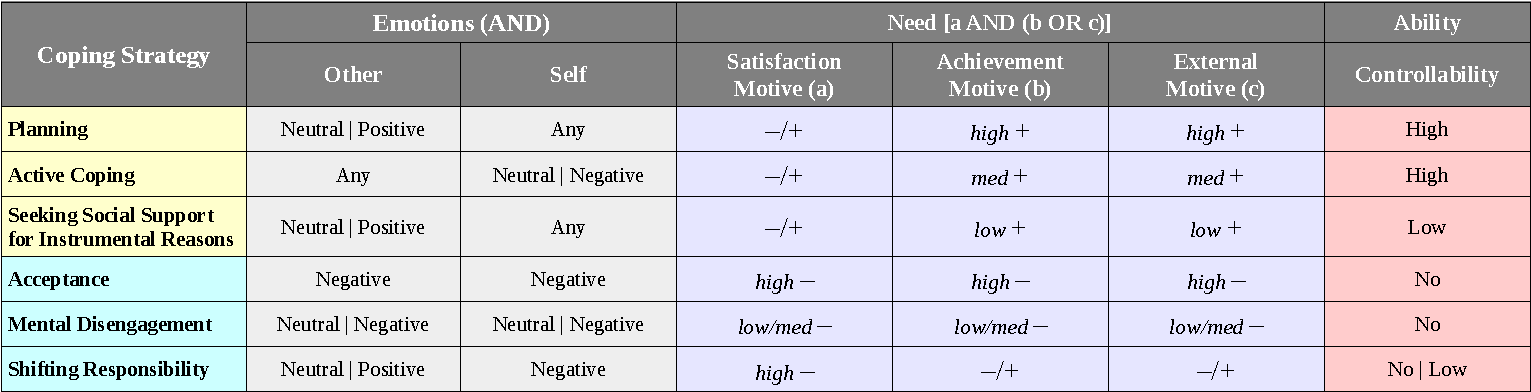
\includegraphics[width=1\textwidth]{figure/coping_algorithms_short_croped.pdf}
\end{sidewaystable}

\subsection{Active Coping}
\label{sec:active-coping}
The \textit{active} coping strategy can provide one or all of the following
three different intentions with respect to whether this coping strategy is
activated and the required conditions are provided. Firstly, this coping
strategy can provide an intention to \textit{acknowledge} the human's emotions.
For instance, if the human expresses an emotion with negative valence, the agent
can acknowledge human's negative emotion accordingly. Secondly, the active
coping strategy can provide an intention to \textit{respond} to the human if
the human asks a question. Currently, in our framework, the agent can respond to
the human if the human asks the agent: a) what input is required to achieve a
goal, b) how to do a task to achieve a goal, c) to achieve a goal, d) who is
responsible to achieve a given goal. For instance, if the human asks the agent
to achieve a goal, the active coping strategy forms an intention to either
accept the human's proposal (if achieving the given goal is controllable for the
agent), or reject the human's proposal (if it is not controllable for the
agent). Thirdly, the active coping strategy can form an intention to
\textit{delegate} a task to the human collaborator. The intention for task
delegation can be formed if the agent fails to achieve its own goal, and the
human's perceived emotion is not negative. As mentioned earlier, any or all of
these intentions can be formed if active coping is selected. The agent acts
accordingly by passing these intentions to the Action mechanism. For instance,
if the human is frustrated about a failure that occurred when using a tool to
perform its own task and asks the agent whether the agent can provide its own
tool, the active coping strategy forms a new intention to acknowledge the
human's frustration and responds to the human by providing the right tool
(input) to use and fulfill the task. In this example, there will be no new
intention to delegate a new goal to the human since the agent perceives the
human's negative emotion.

\subsection{Seeking Social Support for Instrumental Reasons}
The \textit{seeking social support for instrumental reasons} strategy forms new
intentions for the agent whenever the agent needs the human's help and needs to
ask questions from the human collaborator to make progress in collaboration. The
questions that our agent can ask are the reciprocal of those questions that the
human can ask and the human can respond as we mentioned in Section
\ref{sec:active-coping}. Therefore, our agent can ask a) what input is required
to achieve a goal, b) how to do a task to achieve a goal, c) the human to
achieve a goal, d) who is responsible to achieve a given goal. Reciprocally,
again, the agent expects the human collaborator to accept or reject the agent's
proposals. In our framework, whenever this strategy is activated the agent
considers human's perceived emotion. For instance, if the human is worried about
the outcome of a task failure, the agent does not form an intention to ask
questions about any of the above cases and consequently prevents asking for more
help.

\subsection{Acceptance}
The \textit{acceptance} coping strategy forms an intention to drop the
intention of pursuing a goal. In our framework, if this strategy becomes
activated, the intention to pursue the current goal will be dropped; see Table
\ref{fig:coping_strategies}. {\color{red}For instance, if the human has failed
to achieve a goal due to the lack of a required input, and the agent is not able to pursue
another goal and the agent is not able to provide the required input, this
strategy becomes activated.} The acceptance strategy also forms an intention to
inform the human collaborator about the agent's decision on not pursuing the
current goal.

\subsection{Mental Disengagement}
The \textit{mental disengagement} coping strategy forms new intention to lower
the negative emotional intensity associated with a goal in the event of a
failure or an impasse. We use our goal management algorithm (see section
\ref{sec:goal-management}) as the result of selecting this strategy to
dissociate from the current goal in the collaboration process and subsequently
disengage the collaborator from a negative event (e.g., failure to achieve a
goal). This disengagement helps the agent to lower the utility of an
unsuccessful goal achievement attempt and focus on other achievable goals with
respect to their costs to facilitate progress of collaboration. In our
framework, this coping strategy forms an intention to run the goal management
process. As the result of mental disengagement activation, the Coping mechanism
also forms another intention to inform the human about the outcome of the goal
management process, i.e., whether the agent proposes switching to pursue another
goal with lower cost, or if there is not much the agent can do since there is no
other goal with a lower cost to pursue. The process and example of choosing
another goal with a lower cost are shown in Section \ref{sec:goal-management}.

\subsection{Shifting Responsibility}
The \textit{shifting responsibility} strategy forms a new intention to shift the
blame from the agent to another entity. In our framework, we use this strategy
to mitigate the influence of negative events causing negative emotions in the
agent or the human collaborator. For instance, if this strategy becomes
activated as a result of a failure, a new intention will be formed to blame the
other collaborator, or the third person who provided the input (if the task
needed a tool as an input). It can also form an intention to give the credit to
the human collaborator to mitigate human's negative emotions.

\subsection{Activation of Coping Strategies}

In our Coping mechanism, there are three activation criteria for each coping
strategy. The first criterion is the conjunction of emotion valences of the self
and the other collaborator (see Emotion Valence column in Table
\ref{fig:coping_strategies}). For instance, if the valence of the human
collaborator's emotion is \textit{negative} \textbf{and} the valence of the
agent's emotion is also \textit{negative}, the active coping ($2^{nd}$ row), the
acceptance ($4^{th}$ row), and the mental disengagement ($5^{th}$ row) coping
strategies are the coping strategy candidates that have potential to become
activated if the other activation criteria also exist for any of them. For
example, if the human collaborator is frustrated and the agent's elicited
emotion is guilt, the three above mentioned coping strategies become potential
candidates to be selected as the agent's active coping strategy. The second
criterion is the need for the agent to cope with an event. The values of our
three different motives (i.e., \textit{satisfaction}, \textit{achievement}, and
\textit{external}) are involved in the decision of whether there is a need for a
particular coping strategy to become activated. We use conjunction of
satisfaction motive's value with the disjunction of achievement and external
motives. For instance, if we have highly negative values for all three motives
for the potential candidates of coping strategies based on the example we
mentioned above, the acceptance coping strategy will be selected as the strategy
with the highest need for the agent. For example, this kind of condition can
occur when the agent fails doing its own task and pursuing the current goal
(negative satisfaction motive), and can not find another goal to overcome the
impasse (negative achievement motive). The details about how the motive values
are computed is presented in Section \ref{sec:motivation_mechanism}. Finally,
the ability to cope with an event is the third criterion that impacts the
decision of whether the selected coping strategy can be activated. The
controllability of an event represents whether the agent is able to control the
situation occurring with the given event. In our example, if the agent finds the
event uncontrollable, the acceptance coping strategy becomes activated (see
Table \ref{fig:coping_strategies}).

\section{Motivation Mechanism}
\label{sec:motivation_mechanism}
As we discussed in Chapters \ref{ch:background} and \ref{ch:amct}, motives are
goal-driven emotion-regulated constructs indicating an urge related to their
goal. There are several motives in psychological and computational literatures
as we reviewed in Chapter \ref{ch:background}. However, none of these
computational models have particularly focused on the application of motives in
the collaboration context. {\color{red}We believe motives have a key role to
fill the gap between the Appraisal and Coping mechanisms in a collaborative
environment. In fact motives can improve the intention formation process with
respect to the urge of pursuing a goal by considering the emotional states of
the collaborators. As shown in Table \ref{fig:coping_strategies}, it is not
enough to choose a particular coping strategy only by knowing how controllable
is pursuing the given goal. For instance, motive values can help the agent to
choose between \textit{Acceptance} and \textit{Mental Disengagement} when
pursuing a goal is not controllable.}

{\color{red}As mentioned in Chapter \ref{ch:background}, we provided three types
of prominent motives in the literatue; i.e., \textit{achievement, affiliation} and
\textit{power}. However, due to the fact that not all of these motives fit to
the dyadic collaboration context, we developed our own computational models of
motives in our framework, including: \textit{satisfaction},
\textit{achievement}, and \textit{external} motives. Our approach in general is
inspired by the Merrick and Shafi's work in
\cite{merrick:acheievement-affiliation-power} modeling motives using curves
generated by sigmoid functions. In our work, curves are influenced by the
valence of human collaborator's perceived emotion. This section provides more
details about how different curves model different motives in our computational
framework.} We use the values of these three motives in other mechanisms
including the Coping mechanism as we described in Section
\ref{sec:coping-mechanism} and show in Table \ref{fig:coping_strategies}.

\subsection{Satisfaction Motive}
The satisfaction motive indicates the satisfaction level with the collaboration
for the agent and its human collaborator. The satisfaction motive process maintains
the value of \textit{satisfaction drive} throughout the collaboration. The
satisfaction drive is the quantitative weighted accumulation of desirability
values between -1 and +1 over time. For instance, if the desirability values of
the agent's appraisal over three consecutive turns are \{0.75, 0, -0.25\}, and
their corresponding weights are \{0.25, 0.5, 1.0\}, the satisfaction drive value
will be (0.25)(0.75) + (0.5)(0) + (1.0)(-0.25) which is -0.0625. Notice that
the latest desirability values get higher weights. Intuitively, it is because
older desirable events have less influence on overall desirability and
consequently the satisfaction level of the collaboration. The same process
computes the satisfaction drive values for the agent and the human collaborator.
Only the sources of desirability values are different, i.e., appraisal for the
agent and reverse appraisal for the human collaborator. Then, the satisfaction
motive process computes the difference between the current and the previous
(t-1) satisfaction drives, called the delta of satisfaction drive value,
$\delta_{sat}$. As shown in equation \ref{eqn:satisfaction_motive}, we use the
$\delta_{sat}$ value in all three functions to compute the overall satisfaction
motive's value $\mathcal{M}_{sat}$. We also use three different functions with
respect to the valence value of the the human collaborator's perceived emotion.
Our satisfaction motive's model has three domain dependent parameters
$\mathcal{S}_{sat} \in [0, 1.5]$, i.e. strength of motive,
$\mathcal{B}^\mathcal{L}$ where $\mathcal{B}$ is the base parameter of the
function in $(1,\infty)$ and $\mathcal{L}$ is the exponential parameter of the
same function in $(0, \infty)$; together $\mathcal{B}$ and $\mathcal{L}$ define
\textit{unsatisfiability} value. Currently we set $\mathcal{S}_{sat}$ value to
1.5, $\mathcal{B}$ to 3.0, and $\mathcal{L}$ to 2.0.

\begin{equation}
    \mathcal{M}_{sat}(\varepsilon_t)= 
    \begin{dcases}
       arctan (\mathcal{S}_{sat} \times \delta_{sat})      & valence = 0 \\
       \mathcal{B}^{\mathcal{L} \times (\delta_{sat}-1)}   & valence > 0 \\
       -\mathcal{B}^{-\mathcal{L} \times (\delta_{sat}+1)} & valence < 0
    \end{dcases}
    \label{eqn:satisfaction_motive}
\end{equation}

{\color{red}The curves, shown in Figure \ref{fig:satisfaction-motive-functions},
suitably represent the change in magnitude of satisfaction motive based on
different valence values of human collaborators emotion.}
Intuitively, if the human collaborator does not express any emotion, the
satisfaction motive's value can vary between -1 and +1 (blue curve in Figure
\ref{fig:satisfaction-motive-functions}). However, if the agent perceives
positive emotion, there will be no negative satisfaction value since the other
collaborator is in positive state of mind (red curve in Figure
\ref{fig:satisfaction-motive-functions}), and in contrast, if the agent
perceives negative emotion, the satisfaction motive value only changes between
-1 and 0 (green curve in Figure \ref{fig:satisfaction-motive-functions}) with
respect to how satisfied the agent is according to the status of its own goals
during collaboration.

\begin{figure}[tbh]
  \centering
  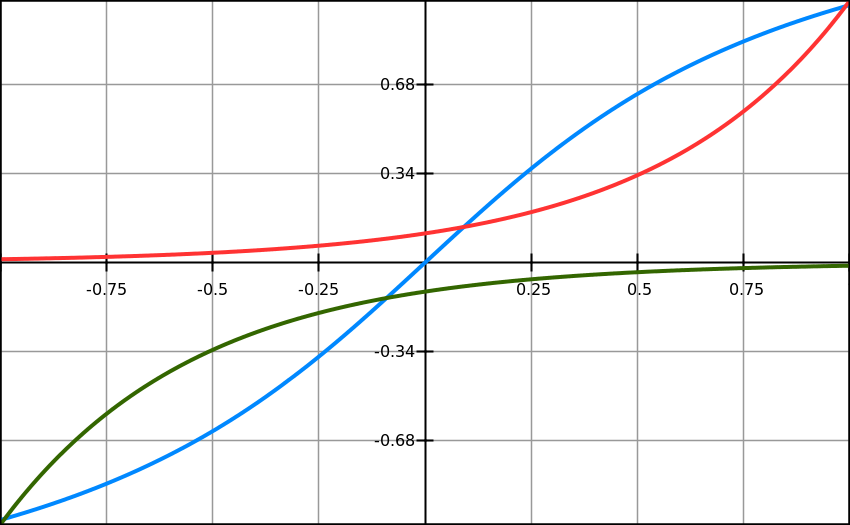
\includegraphics[width=1\textwidth]{figure/satisfaction_motive_functions.png}
  \caption{Three functions of satisfaction motive for different values of
  valence (blue: valence = 0, red: valence = positive, green: valence =
  negative). The x-axis indicates the satisfaction drive's delta value in [-1,
  +1], and the y-axis indicates the magnitude of satisfaction motive in [-1,
  +1].}
  \label{fig:satisfaction-motive-functions}
\end{figure}

\subsection{Achievement Motive}
The achievement motive drives the agent's need to achieve a goal during the
collaboration. According to the literature, e.g.
\cite{merrick:acheievement-affiliation-power}, the achievement motive is based
on the estimation of success probability and the difficulty of achieving a goal.
In our framework, we compute the probability of success as the product of the
\textit{controllability} and \textit{expectedness} appraisal values.
Intuitively, the more controllable and expected the events are, the probability
of successful achievement of their related goal is higher.

\begin{figure}[tbh]
  \centering
  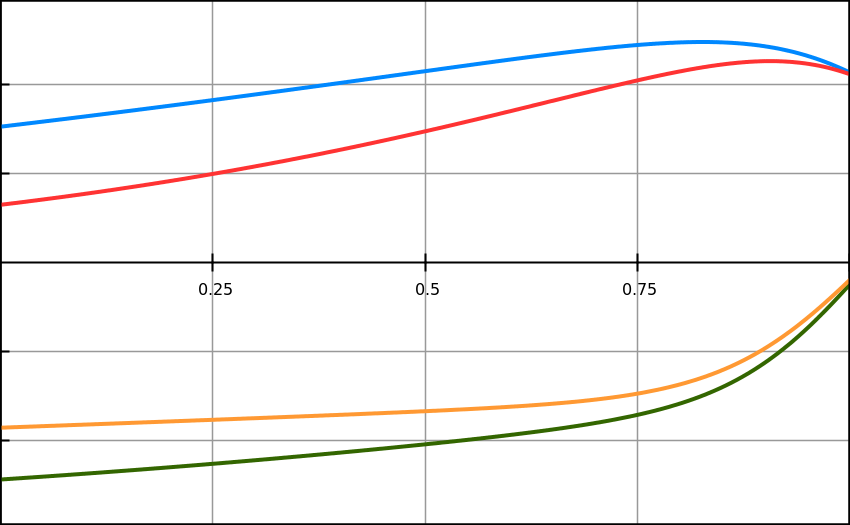
\includegraphics[width=1\textwidth]{figure/achievement_motive_functions.png}
  \caption{Two functions of the achievement motive for different values of
  valence (blue: valence = +1, red: valence = 0, green: valence = -1, orange:
  valence = close to zero from negative side). The x-axis indicates the success
  probability value of achieving a goal which is in [0, +1], and the y-axis
  indicates the magnitude of achievement motive in [-1, +1].}
  \label{fig:achievement-motive-functions}
\end{figure}

In our framework we use two sigmoid-based functions to compute the achievement
motive's value. These functions values change based on the probability of
success and valence of the human collaborator's emotion. We use Equation
\ref{eqn:achievement-motive-valence-positive} when the perceived emotion of the
human has positive or zero valence value, and we use Equation
\ref{eqn:achievement-motive-valence-negative} when the perceived emotion
of the human has a negative valence value. As shown in Figure
\ref{fig:achievement-motive-functions}, when the value of the valence changes
between 0 and +1, the output of $\mathcal{M^{+}}_{ach}$ function changes between
the red and the blue lines respectively. Conversely, when the value of the
valence changes between -1 and a small negative number (close to zero), the
output of $\mathcal{M^{-}}_{ach}$ function changes between the green and the
orange lines.

\begin{equation}
\mathcal{M^{+}}_{ach}(\varepsilon_t)=
\frac{2.0}{1+e^{(2.0-valence)\times(1.05-p(success))}}
- \frac{1.0}{1+e^{(12.0-valence)\times(1.2-p(success))}}
\label{eqn:achievement-motive-valence-positive}
\end{equation}

\begin{equation}
\mathcal{M^{-}}_{ach}(\varepsilon_t)=
\frac{1.0}{1+e^{(0.5+valence)\times(1.05)-p(success)}}
- \frac{1.0}{1+e^{(12.0+valence)\times(p(success)-1.02)}}
\label{eqn:achievement-motive-valence-negative}
\end{equation}

By intuition, as the probability of success increases the agent is more
motivated to achieve a goal and this motive gets higher when the human's
emotion is positive or at least neutral. The human's negative emotions cause
lower values of achievement motive since taking care of and acknowledging the
human's negative emotion should have higher priority for a collaborative agent
than achieving a goal.

\subsection{External Motive}
The external motive drives the agent's need to achieve a proposed goal by the
human collaborator during the collaboration. In our framework, the external
motive is also based on the estimation of success probability and the difficulty
of achieving a goal, but this goal is proposed by the human collaborator. The
probability of success for the external motive is computed the same way as the
achievement motive's probability of success, i.e. the product of
\textit{controllability} and \textit{expectedness} appraisal values.

The only difference from the achievement motive is that we use Equations
\ref{eqn:achievement-motive-valence-positive} and
\ref{eqn:achievement-motive-valence-negative} in reverse order for the external
motive; i.e., we use Equation \ref{eqn:achievement-motive-valence-negative}
when the valence of human's perceived emotion is positive, and Equation
\ref{eqn:achievement-motive-valence-positive} when the valence of the human's
perceived emotion is negative or zero.

\begin{figure}[tbh]
  \centering
  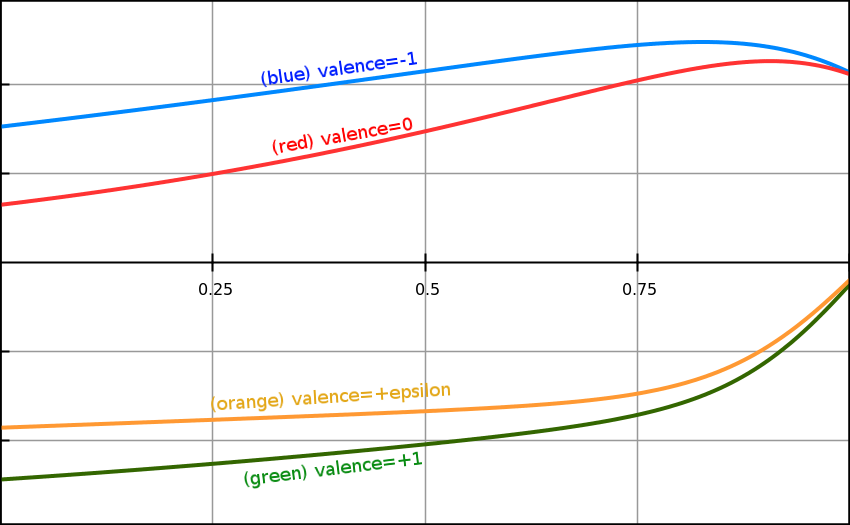
\includegraphics[width=1\textwidth]{figure/external_motive_functions.png}
  \caption{Two functions of external motive for different values of valence
  (blue: valence = -1, red: valence = 0, green: valence = +1, orange: valence =
  close to zero from negative side). The x-axis indicates the success
  probability value of achieving a proposed goal which is in [0, +1], and the
  y-axis indicates the magnitude of the achievement motive in [-1, +1].}
  \label{fig:external-motive-functions}
\end{figure}

Intuitively, when the human proposes a new goal while expressing a negative
emotion the agent should be more motivated to acknowledge human's proposal and
pursue the proposed goal to mitigate human's negative emotion and maintain the
collaboration. {\color{red}For example, when the human collaborator is worried
about the failure of attaching a solar panel due to a malfunction of a tool,
and proposes the robot to attach the panel, the high value of the external
motive causes the robot to accept the human's proposal.}

\section{Theory of Mind}
\label{sec:theory-of-mind-implementation}
{\color{red}The Theory of Mind mechanism uses the collaboration structure and
functions described in Section \ref{sec:collaboration-mechanism} as well as appraisal
processes to form anticipated beliefs about the human's mental and emotional
states. In other words, since our agent knows about the human's goals (as part
of the shared plan), it can apply the human goals to the same algorithms during
the human's turn of the collaboration. The agent uses the collaboration
structure during the human's turn to compute appraisal values with respect to
the human's current emotional state and the current goal in the shared goal
structure. The outcome of the reverse appraisal forms beliefs about the
anticipated mental and emotional state of the human collaborator.

\subsubsection{Reverse Appraisal}
We use the same \textit{relevance}, \textit{expectedness} and
\textit{controllability} algorithms for the reverse appraisal as those
algorithms we described in Section \ref{sec:appraisal}. In these three
algorithms the Theory of Mind mechanism substitutes the agent's required goal
and its corresponding constraints and information with the human's goal and its
corresponding information which is provided to the agent within the shared plan
structure.  However, only for the reverse appraisal of \textit{desirability} we
chose to simply use the valence value of the human's perceived emotion and
interpret negative, neutral and positive valence values as undesirable, neutral
and desirable values respectively. In this way, our agent could directly infer
whether the occurrence of the current event and its corresponding goal is
desirable for the human. The outcome of all of these processes is a vector of
reverse appraisal values that could be used by other mechanisms in our
framework.}

\section{Elicitation of Emotion Instances}
We have modeled 10 different emotion instances that can be elicited by the agent
or anticipated from the human during collaboration in our framework (see Table
\ref{fig:emotion_elicitation}). {\color{red}We chose these 10 emotions because
we believe they are good examples of social emotions that can occur during a
collaboration.} These emotion instances have meanings in social context and more
specifically in collaboration. There are two components involved in selecting a
particular emotion: appraisal variables and collaboration context.

We use the outcome of the four appraisal processes discussed in section
\ref{sec:appraisal} to determine the potential emotion instance to be elicited
(if the agent wants to express an emotion), or to anticipate a potential emotion
from the human collaborator (if the human response is anticipated). The outcome
of appraisal processes can be one of the values presented in Table
\ref{fig:appraisal_values} with respect to the corresponding process.
{\color{red}For instance, relevance can only obtain either of two values,
i.e., \textsc{relevant} or \textsc{irrelevant}., or the controllability can
obtain one of the three values in Table \ref{fig:appraisal_values}; i.e.,
\textsc{high\_controllable, low\_controllable} or \textsc{uncontrollable}.}

\vspace*{5mm}
\begin{table}[tbh]
  \centering
  \caption{Appraisal values for relevance, desirability, expectedness and
  controllability.}
  \label{fig:appraisal_values}
  \vspace*{-3mm}
  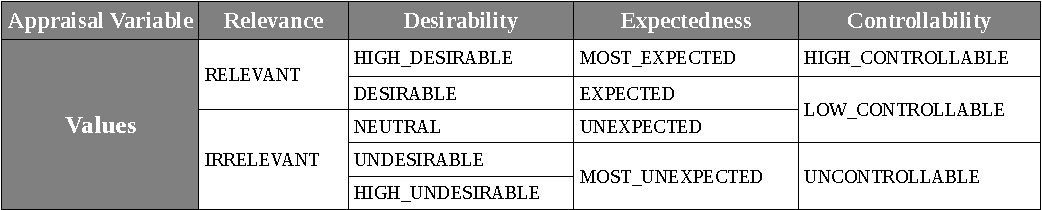
\includegraphics[width=1\textwidth]{figure/apraisal_values_croped.pdf}
\end{table}

We also use the collaboration context as our second determinant to select a
particular emotion. We define the collaboration context based on: \textit{goal
achievement} (\textsc{human\_achieved} and \textsc{agent\_achieved}),
\textit{goal failure} (\textsc{human\_failed} and \textsc{agent\_failed}),
\textit{proposal of a goal} (\textsc{human\_proposed} and
\textsc{agent\_proposed}), \textit{acceptance of the proposed goal}
(\textsc{human\_accepted} and \textsc{agent\_accepted}), and \textit{rejection
of the proposed goal} (\textsc{human\_rejected} and \textsc{agent\_rejected}).
All of these situations can occur by either of the collaborators, i.e., agent or
human (see Table \ref{fig:emotion_elicitation}). There is only one exception
and it is when the desirability value is neutral the associated emotion to the
event is always neutral without considering the collaboration context and the
values of other appraisal variables (see first row in Table
\ref{fig:emotion_elicitation})\footnote{{\color{red}Empty cell in Table
\ref{fig:emotion_elicitation} indicate that the value of the cell does not
influence the selection of the emotion in the corresponding row.}}.
{\color{red}In summary, the outcome of four appraisal processes and the inferred
context of a collaboration can lead the agent to elicit its own emotion or
anticipate the human collaborator's emotion.}

{\color{red} In the following interaction based on our example scenario in
Section \ref{sec:example-scenario}:\\

  5. \textbf{\textit{Astronaut}}: The connectors on this panel have problems and
  we might not be able to finish this task.

  6. \textbf{\textit{Robot}}: Don't worry! I can replace the connectors in 4
  minutes. We definitely can finish this task after that.\\

The agent finds the Astronaut's goal \textsc{uncontrollable},
\textsc{unexpected}, \textsc{undesirable} and \textsc{relevant} (see all
possible values of appraisal variables in Table \ref{fig:appraisal_values}).
Also, the agent finds the current context of collaboration as
\textsc{human\_proposed}; therefore, the agent infers that Astronaut's
perceived negative emotion instance can be \textit{worry}. Thus, since the agent
have access to working connectors (required inputs to the Astronaut's task),
first, the agent acknowledges the Astronaut's negative emotion, then informs
the Astronaut with proper solution to mitigate the Astronaut's negative
emotion.}


\begin{sidewaystable}
  \centering
  \caption{Conditions for selecting emotion instances.}
  \label{fig:emotion_elicitation}
  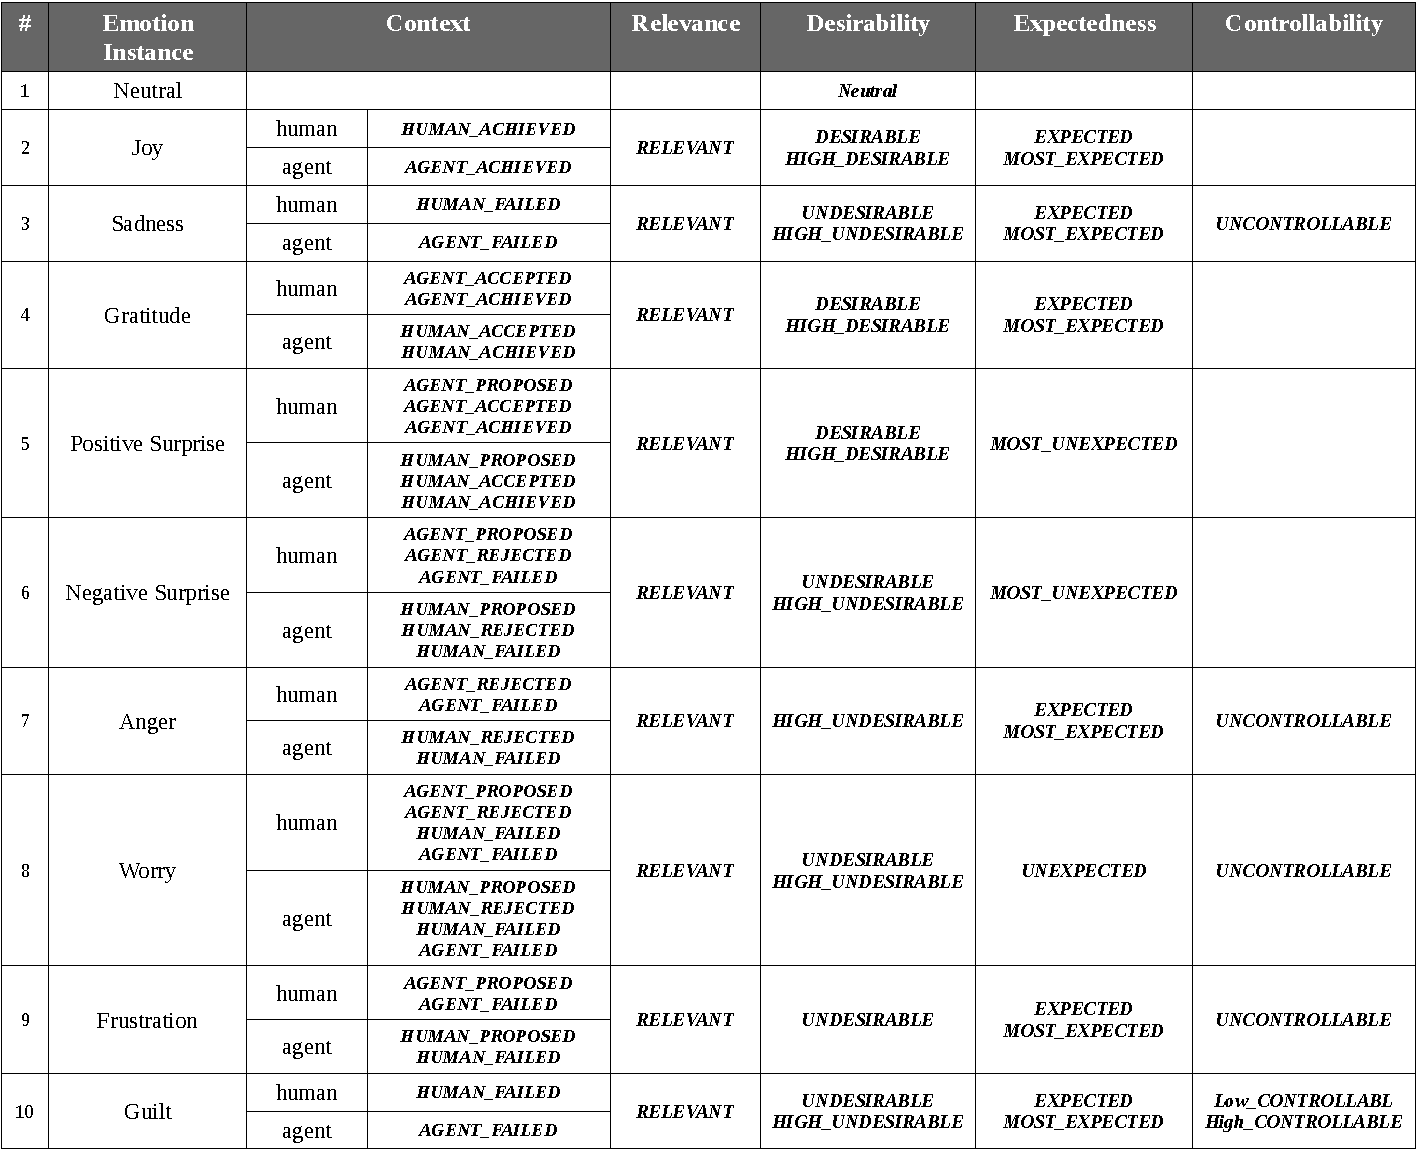
\includegraphics[width=1\textwidth]{figure/emotion_elicitation_croped.pdf}
\end{sidewaystable}

\chapter{Evaluation}
\label{ch:awareness}

In this chapter, we provide the explanation and results of two different user
studies. The first user study (see Section \ref{sec:crowd-sourcing}) was
conducted online to evaluate our appraisal algorithms. Specifically, the goal of
this study was to validate the effectiveness of the factors involved in our
appraisal algorithms. We prepared online questionnaires and asked participants
to tell us what their decision would be in the simple situations provided. The
participants' answers to our questionnaires were compared with the results of
our algorithms for the given situations. The results are provided in Section
\ref{sec:crowd-sourcing}. The second user study (see Section
\ref{sec:end-to-end}) was conducted in the laboratory The goal of this user
study was to provide an end-to-end system evaluation using our overall
framework. We provided pre- and post-study questionnaires as well as an
open-ended questionnaire to study the humans' evaluation of a robot
collaborating using our framework. The results are provided in Section
\ref{sec:end-to-end}.

\section{Implementation}
As described in Chapter \ref{ch:amct}, the Perception and Action mechanisms are
not part of our theoretical work. Therefore, we only implemented these
mechanisms to the extent to which they could help us to run and test our
framework. The Perception mechanism only redirects the input values from the
system's users to the framework. For instance, in our user study described in
Section \ref{sec:end-to-end}, the Perception mechanism only receives the valence
of human's emotion from the input and provides it to the framework.
On the other hand, the Action mechanism executes some functions based on the
intentions formed and provided by the Coping mechanism described in this
section. We group all of these functions into three categories in our framework.
The first group of functions includes all of the functions capable of executing
some actions with respect to the domain. The second category includes all of the
functions involved in revealing the agent's utterances by writing on the screen or
conveying through the agent's voice and text to speech systems. The last
category includes all of the functions to express the agent's emotion. The
emotions can be expressed through colors, emoticons, voice and text. For
example, in the user study described in Chapter \ref{ch:awareness}, we expressed
the agent's emotions by using emoticons and utterances through the text on the
screen as well as the agent's voice.

\section{Evaluating Appraisal Algorithms (Crowd Sourcing)}
\label{sec:crowd-sourcing}
In this section, we present a crowd-sourced user study and the results, which
we conducted to validate the components of our appraisal processes.

\subsection{Experimental Scenario}
We developed an experimental scenario in which participants were asked to
envision a sequence of hypothetical collaborative tasks between themselves and
an imaginary friend, Mary, in order to accomplish their shared goal. To minimize
the background knowledge necessary for our test subjects, we used a simple
domestic example of preparing a peanut butter and jelly sandwich, and a hard
boiled egg sandwich for a hiking trip. The tasks did not require the
participants to do any deep problem solving; rather, the tasks were part of
simple daily activities that should be familiar to all participants. 
% 
% \subsection{Tasks}
% Participants were asked to carry out a sequence of hypothetical collaborative
% tasks between them and an imaginary friend, Mary, in order to accomplish their
% goal of preparing two sandwiches. All the tasks were simple and did not require
% the participants to solve a particular problem rather accomplish something as
% they do in their day to day life.
% 
% \section{Evaluation}

\subsection{Hypothesis and Methodology}

\subsubsection{Hypothesis}
We conducted this user study to test our hypothesis that humans and our
algorithms will provide similar answers to questions related to different
factors used to compute four appraisal variables: relevance, desirability,
expectedness, and controllability.

\begin{figure*}[tbh]
  \centering
  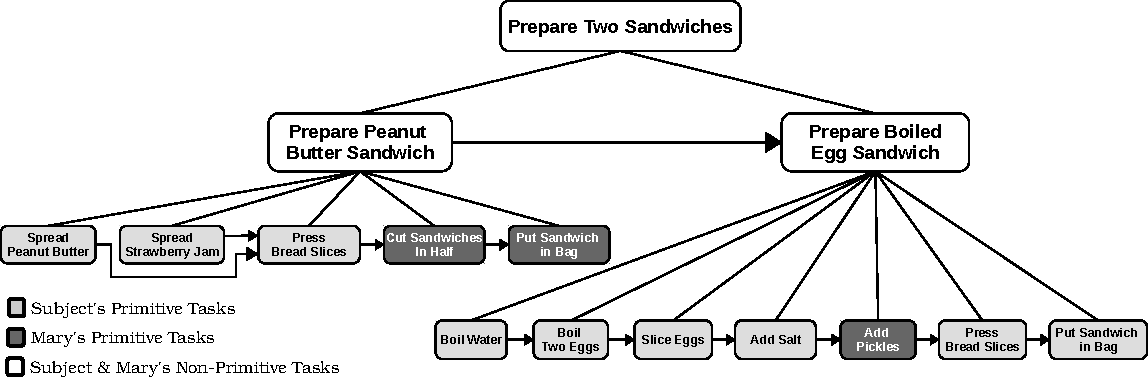
\includegraphics[width=1\textwidth]{figure/taskModel-croped.pdf}
  \caption{Collaboration task model for the evaluation.}
  \label{fig:taskModel}
\end{figure*}

\subsubsection{Procedure}
 We conducted a between-subject user study using an online crowdsourcing website
 -- CrowdFlower\footnote{http://www.crowdflower.com}. We had a questionnaire for
 each appraisal variable. There were 12 questions (including 2 test questions)
 in the controllability and expectedness questionnaires, 14 questions (including
 2 test questions) in the desirability questionnaire, and 22 questions
 (including 3 test questions) in the relevance questionnaire.
 
We provided textual and graphical instructions for all questionnaires; Figure
\ref{fig:taskModel} shows the corresponding task
model\footnote{{\color{red}Figure \ref{fig:taskModel} was not given to the
participants.}}. The instructions, provided in the Appendix A, presented a
sequence of hypothetical collaborative tasks to be carried out by the test subject and an imaginary friend, Mary, in
order to accomplish their goal of preparing two sandwiches. We also provided a
simple definition and an example of each appraisal variable. The collaboration
structure and the instructions were the same for all questionnaires. The
questions introduced specific situations related to the shared plan, which
included blocked tasks and failure or achievement of a shared goal. Each
question provided three answers which were counterbalanced in the questionnaire.
We provided an option like C in all questions (see Figure \ref{fig:qs1}),
because we did not want to force participants to choose between two options when
they did not have a good reason. {\color{red}We derived two questions for
different factors invoved in each algorithm (see Section \ref{sec:appraisal}).
For instance, we prepared two questions about the influence of the strength of a
belief as a key factor involved in relevance algorithm.} The questions were
randomly placed in the questionnaire. Figure \ref{fig:qs1} shows an example
question from the relevance questionnaire which was designed to test whether
participants perceive saliency as a factor in relevance. The input for our
algorithms was the task model depicted in Figure \ref{fig:taskModel}.

\subsubsection{Participants}
Each participant group originally had 40 participants. We limited the
participant pools to those with the highest confidence level on the
crowdsourcing website in the United States, Britain, and Australia. Test
questions were included to check the sanity of the answers. We eliminated
participants providing wrong answers to our sanity questions, and participants with
answering times less than 2 minutes. The final number of accepted participants
in each group is provided in Table \ref{tbl:statistics}.

\begin{table}[htbp]
\centering
\caption{Number of participants}
\begin{tabular}{|c|c|c|c|c|} \hline
appraisal variables & \# of participants\\ \hline 
Relevance &  29\\ \hline
Desirability & 35\\ \hline 
Expectedness & 33\\ \hline 
Controllability & 33\\ \hline
\end{tabular}
\label{tbl:statistics}
\end{table}

% \begin{table}[htbp]
% \vspace*{-3mm}
% \centering
% \caption{Number of Participants}
% \begin{tabular}{|c|c|c|c|c|} \hline
% appraisal variables & \# of participants & mean & stdev & \textit{p}-value\\ \hline 
% Relevance &  29 & 0.713 & 0.107 & $<$0.001\\ \hline
% Desirability & 35 & 0.778 & 0.150 & $<$0.001\\ \hline 
% Expectedness & 33 & 0.785 & 0.120 & $<$0.001\\ \hline 
% Controllability & 33 & 0.743 & 0.158 & $<$0.001\\ \hline
% \end{tabular}
% \label{tbl:statistics}
% \vspace*{-3mm}
% \end{table}
% 

\subsection{Results}
\label{sec:results-crowdsourcing}
Each question in our questionnaires was designed based on different factors that
we use in our algorithms (see Section \ref{sec:appraisal}).  For each of the
four questionnaires we provide an example question, and describe how each
question relates to a specific factor within the corresponding algorithm. The
input for our algorithms was the task model depicted in Figure
\ref{fig:taskModel}. The complete list of questions is provided in the Appendix
A. Additionally, we provide the p-value for each question, using a binomial
distribution, with a probability of success of 0.33, which is the probability of
selecting the right answer if the participant is simply guessing.

\subsubsection{Expectedness}
\label{sec:expectedness-crowdsourcing}
Figure \ref{fig:qs1} shows an example question from the expectedness
questionnaire. In this example, with respect to Algorithm \ref{alg:expectedness}
(line 6), option A is more expected because the task related to this option
provides the next available task in the focus stack (see the task model in
Figure \ref{fig:taskModel}). Although the task in option B is part of the
existing task model, it is considered as \textsc{unexpected} by our algorithm,
since it is not live in the plan. We provided option C to determine whether the
participants will differentiate between these two options. This question was
presented to the participants to determine whether their decision for the
expectedness of this event is similar to the output of the expectedness
algorithm. For this question, the human decision was 97\% similar to the
algorithm's output.

\vspace*{3mm}
\begin{table}[tbh]
  \centering
  \caption{Expectedness results {\color{red}(Equally Expected column indicates
  for which questions our algorithm provides option C as the response)}.}
  \label{fig:expectedness_result}
  \vspace*{-3mm}
  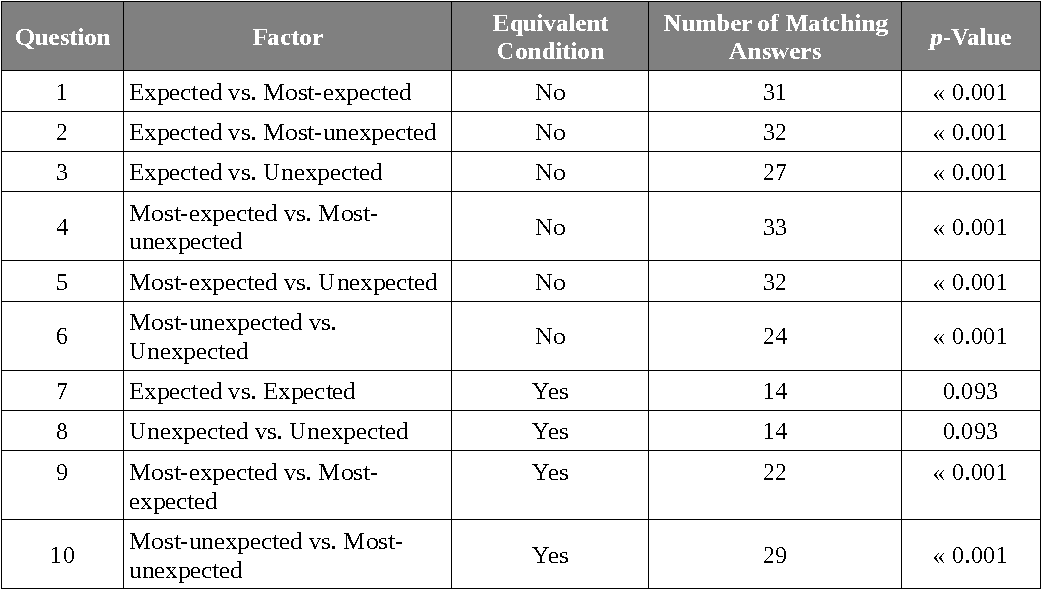
\includegraphics[width=1\textwidth]{figure/expectedness_result_croped.pdf}
\end{table}

Results for the expectedness questionnaire are presented in Table
\ref{fig:expectedness_result}. As shown in this table, the results are
statistically significant; in fact, for questions 1-6 and 9-10, human
participants showed between 67 and 100 \% agreement with our algorithms, with
p-values of $\ll$0.001. Questions 7 and 8 were the only two questions that did
not show a statistically significant p-value. It should be noted that these
questions are comparing equally expected or equally unexpected situations, none
of which our algorithms would consider most-expected or most-unexpected.


\begin{figure}[tbh]
  \centering
  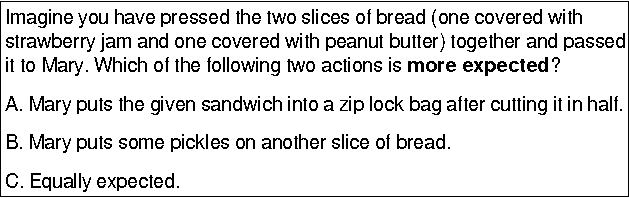
\includegraphics[width=0.85\textwidth]{figure/question-sample-croped.pdf}
  \caption{{Example expectedness question.}}
  \label{fig:qs1}
\end{figure}

\subsubsection{Controllability}
\label{sec:controllability-crowdsourcing}
Figure \ref{fig:qs2} shows an example question from the controllability
questionnaire. The algorithm's output is option B, and is determined by
Algorithm \ref{alg:controllability} (line 3), similarly to the expectedness
example above. In this example, option B is more controllable than option A,
because the self over total ratio of the responsibility of the predecessors of
the given task (see \textit{Autonomy} in Section \ref{sec:controllability}) is
higher than the ratio in option A, i.e., self is responsible to spread peanut
butter on one slice of bread and strawberry jam on another slice of bread. In
this question, the humans decision was 90\% in agreement with the algorithm's
output.

\vspace*{3mm}
\begin{table}[tbh]
  \centering
  \caption{Controllability results {\color{red}(Equally Controllable column
  indicates for which questions our algorithm provides option C as the response)}.}
  \label{fig:controllability_result}
  \vspace*{-3mm}
  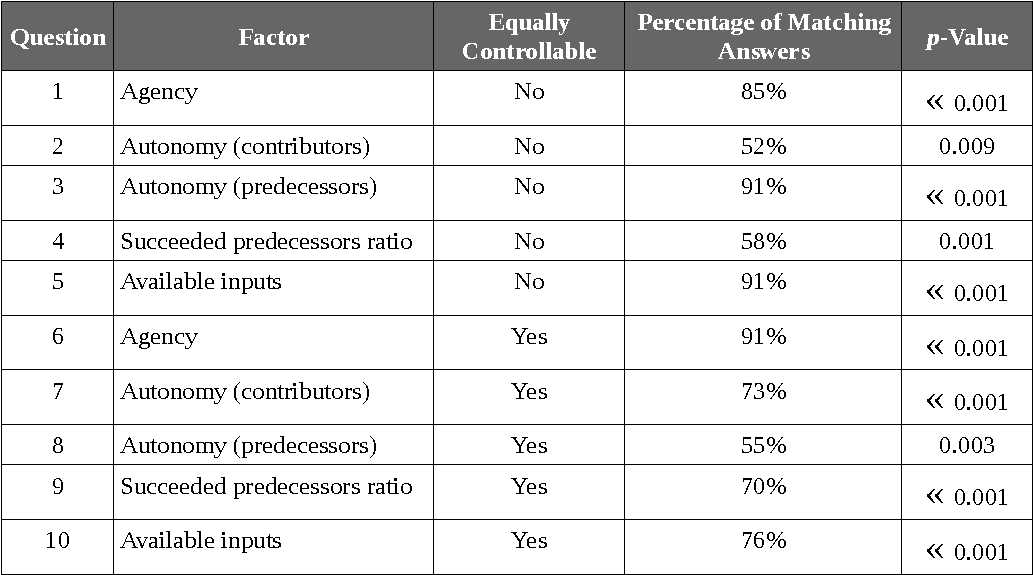
\includegraphics[width=1\textwidth]{figure/controllability_result_croped.pdf}
\end{table}

Results for the controllability questionnaire are presented in Table
\ref{fig:controllability_result}. As shown in the table, the p-value is $<$0.01
for each of the ten questions. The two questions with the lowest human agreement
with the algorithms both relate to autonomy (Questions \#2 and \#8) of the
participants with 52\% and 55\%.

\begin{figure}[tbh]
  \centering
  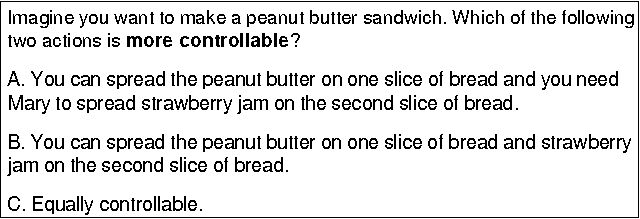
\includegraphics[width=0.85\textwidth]{figure/question-sample2-croped.pdf}
  \caption{{Example controllability question.}}
  \label{fig:qs2}
\end{figure}

\subsubsection{Desirability}
\label{sec:desirability-crowdsourcing}
Figure \ref{fig:qs3} shows an example question from the desirability
questionnaire. The output based on the Algorithm \ref{alg:desirability}
(line 14) is option C, since in both option A and option B, the focus goal
has been achieved successfully. Therefore, in this example, both options A and B
are desirable. The humans' decision was 77\% in agreement with the algorithm's
output in this question.

\begin{table}[tbh]
  \centering
  \caption{Desirability results {\color{red}(Equally Desirable column indicates
  for which questions our algorithm provides option C as the response)}.}
  \label{fig:desirability_result}
  \vspace*{-3mm}
  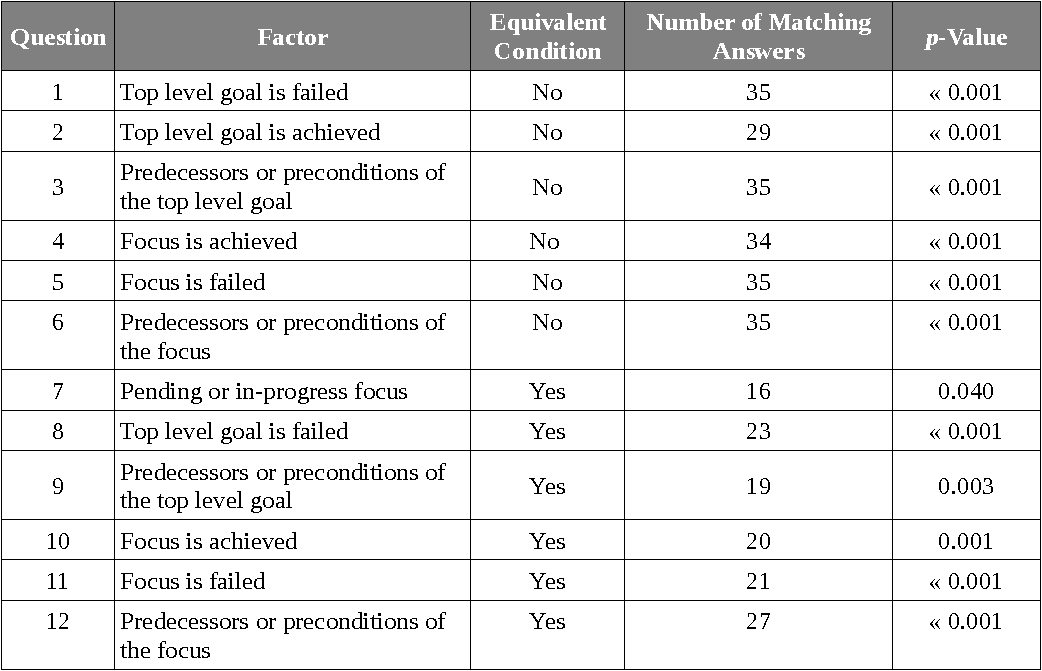
\includegraphics[width=1\textwidth]{figure/desirability_result_croped.pdf}
\end{table}

The results of the desirability questionnaire are presented in Table
\ref{fig:desirability_result}. As shown in the results table, the p-value is
less than 0.05 for all of the desirability questions. However, an interesting
trend is that human participants had a level of agreement of 83\%-100\% when the
algorithm's output selected one alternate as more desirable than another
alternate. When the algorithm's output chose option C (i.e. rating two
situations as equally desirable), the human participants only showed 46\%-77\%
agreement. This may indicate that a higher level of granularity is required in
the algorithm when evaluating options with similar levels of desirability.

\begin{figure}[tbh]
  \centering
  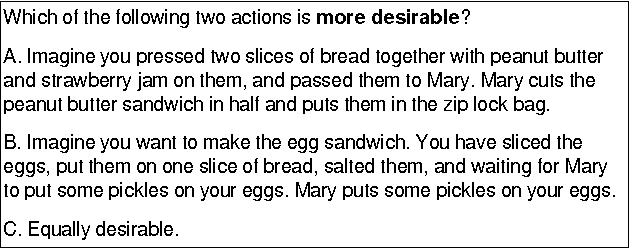
\includegraphics[width=0.85\textwidth]{figure/question-sample3-croped.pdf}
  \caption{{Example desirability question.}}
  \label{fig:qs3}
\end{figure}

\subsubsection{Relevance}
\label{sec:relevance-crowdsourcing}
In the example shown in Figure \ref{fig:qs4}, with respect to Algorithm
\ref{alg:relevance}, option A is relevant because of Mary's perceived negative
emotion (see Equation \ref{eqn:utility}). Although option B is relevant (since
it achieves the next goal in the shared plan), 83\% of participants consider it as
less relevant than option A; we believe this is due to the effect of Mary's
perceived negative emotion which also generates a higher utility value in our
relevance algorithm. Another question also tested belief saliency. However, the
options provided only related to the shared plan (i.e., no human emotions in the
options). In this case 87\% of participants chose the option that accomplished the
next goal in the shared plan. Interestingly, when confronted with a negative
emotion from their collaborator, human participants deviated from the shared plan
and found their collaborator's emotion more relevant than the original plan. It
is noteworthy that in both the absence and the presence of emotions the
participants chose the more salient option with respect to our definition of
saliency, which was not referenced or provided in the questionnaire.

\begin{table}[tbh]
  \centering
  \caption{Relevance results {\color{red}(Equally Relevant column indicates
  for which questions our algorithm provides option C as the response)}.}
  \label{fig:relevance_result}
  \vspace*{-3mm}
  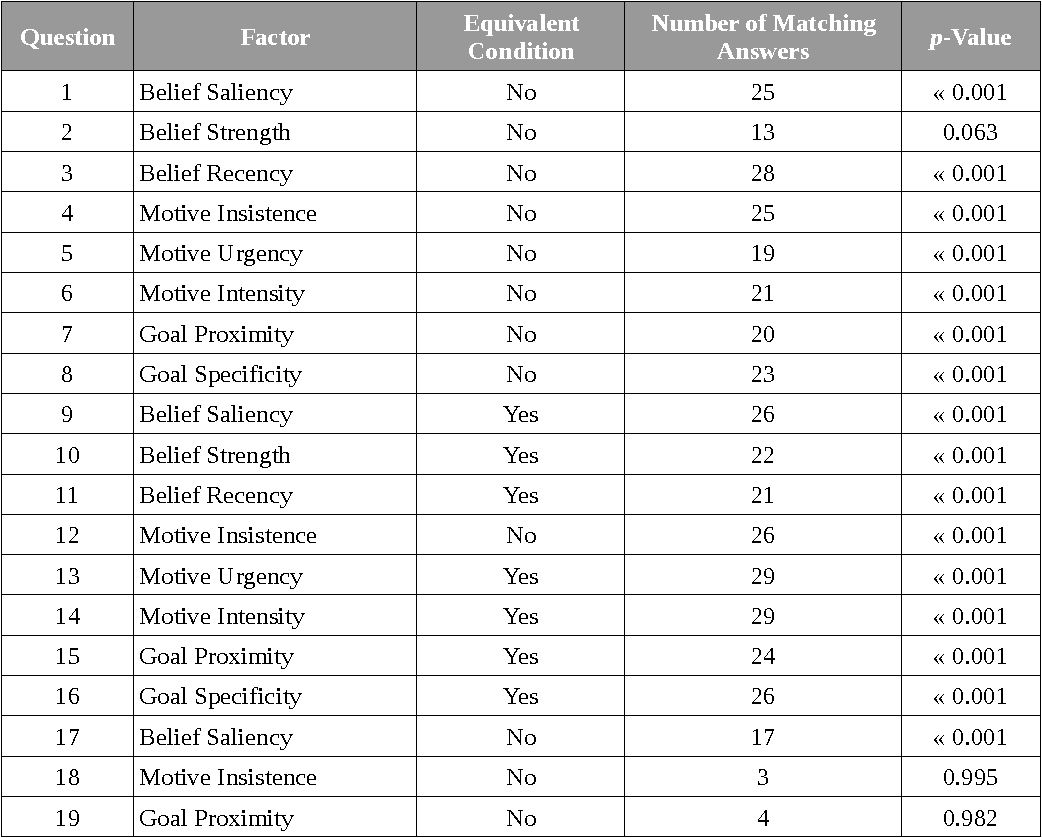
\includegraphics[width=1\textwidth]{figure/relevance_result_croped.pdf}
\end{table}

The complete summary of results for the relevance questionnaire is provided in
Table \ref{fig:relevance_result}. As shown in the table, all questions show
59\%-100\% agreement with our algorithms and statistically significant p-values
except for questions 2, 18 and 19. Question 2 addresses belief strength.
{\color{red} This question presents a situation in which participants must
choose whether a self related goal, or collaborator's goal is more relevant.}
Questions 18 and 19 address motive insistence and goal proximity, respectively;
both of these questions present situations in which participants must choose
whether an intense emotional circumstance, or adherence to the collaboration
plan is more relevant (the questionnaire is provided in the Appendix A). Our
algorithms choose that the strong emotional circumstance will be more relevant;
however, human participants generally selected adherence to the collaboration
plan to be more relevant.

\begin{figure}[tbh]
  \centering
  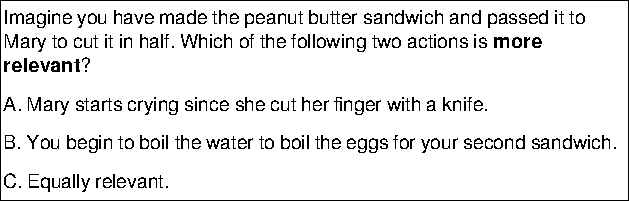
\includegraphics[width=0.85\textwidth]{figure/question-sample4-croped.pdf}
  \caption{{Example relevance question.}}
  \label{fig:qs4}
\end{figure}

\subsection{Discussion}
\label{sec:discussion-crowdsourcing}
As shown in the preceding results tables, the human participants agreed 100\%
on some questions, while on some other questions there was a much lower level of
agreement. Our results indicate that people largely performed as our hypothesis
predicted. The very small \textit{p}-values indicate that the data set is not
random; in fact, the high percentage of similarity confirms our hypothesis and
shows that the algorithms can help us to model appraisal in a collaboration. The
very low level of agreement on a handful of questions may indicate algorithm
components that require further refinement before implementation. {\color{red}We
made changes to our algorithms in light of this study.}

% \section{Conclusions}
% \label{sec:conclusions-crowdsourcing}


% \section{Improving Human-Robot Collaboration Using Emotional-Awareness}
\section{End-to-End System Evaluation}
\label{sec:end-to-end}

As mentioned earlier, collaborative robots need to take into account humans'
internal states while making decisions during collaboration. Humans express
emotions to reveal their internal states in social contexts including
collaboration \cite{breazeal:sociable-interactive-robots}. Due to the existence
of such expressions, robots' emotional-awareness can improve the quality of
collaboration in terms of humans' perception of performance and preferences.
Hence, collaborative robots need to include affect-driven mechanisms in their
decision-making processes to be able to interpret and generate appropriate
responses and behaviors. Our aim in this experiment was to study the importance
of emotional awareness and the underlying affect-driven processes in human-robot
collaboration. We examined how emotional-awareness impacts different aspects of
humans' preferences by comparing the results from our participants collaborating
with an emotion-aware versus an emotion-ignorant robot.

% \section{Collaborative Behaviors and Emotional-Awareness}
% 
% \subsection{Goal Postponement}
% 
% \subsection{Goal Management}
% 
% \subsection{Task Delegation}
% 
\subsection{Experimental Setup}
The setup of this user study included three separate parts. The first
part incorporated the Affective Motivational Collaboration framework consisting
of all Mental Processes (see left-side of Figure \ref{fig:framework}) as we
described in Chapters \ref{ch:amct} and \ref{ch:appraisals}. The second part was
implemented to receive action commands from the framework and forward them to
the robot to control joints and actuators (see right-side of Figure
\ref{fig:framework}). A wizard was the third part of this setting. The wizard
did nothing but inform the robot/framework whether the current task performed by
either the robot or the participant was achieved successfully. The wizard was
completely invisible to the participants, and the wizard had no impact on the
robot's decision other than providing input regarding tasks' failure or success.

\begin{figure*}[tbh]
  \centering
  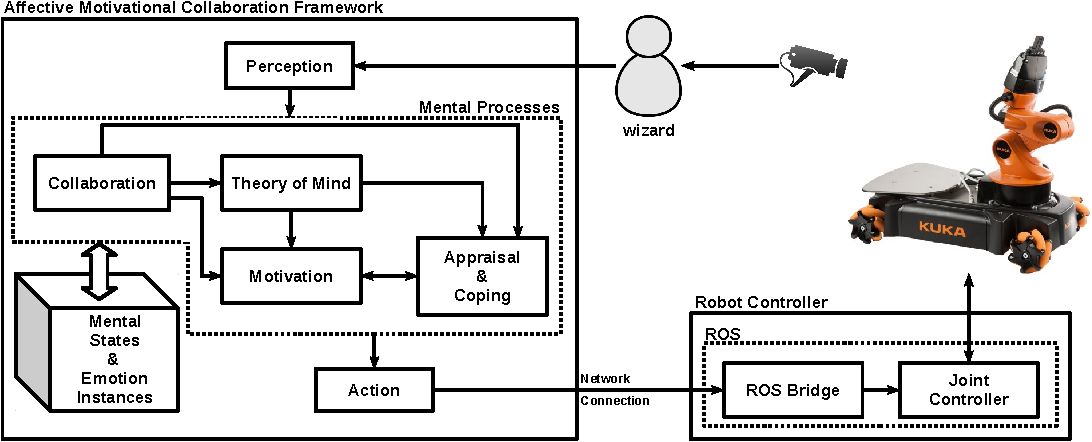
\includegraphics[width=\textwidth]{figure/framework-croped.pdf}
  \caption{Experimental setup for end-to-end system evaluation.}
  \label{fig:framework}
\end{figure*}

\subsubsection{Environment and Tasks}

The environment was set up in a laboratory and included the robot, the
collaboration board on top of a desk, and the participant standing in front of
the robot on the other side of the board (see Figure \ref{fig:environment}). One
of the experimenters monitored the interactions using a live stream of a camera
in a different room. The experimenter provided only the required perception,
i.e., decision on success or failure of the tasks for the robot, through the
entire time of the collaboration (see Section \ref{sec-interaction-paradigms}).
{\color{red}We also had a supervisor, whose purpose was to provide help to the
collaborators when requested after a task failure.}

The tasks were defined based on the collaboration structure shown in Figure
\ref{fig:collaboration_structure} and were executed in a turn-taking fashion by
either of the collaborators\footnote{{\color{red}Figure
\ref{fig:collaboration_structure} was not given to the participants.}}. For each
task either the robot or the participant was responsible for picking up one of
the corresponding pegs from their own inventory and placing it on the right spot
which was colored and tagged the same as the associated peg. Some pegs and
corresponding spots on the board had hidden magnets which prevented the pegs
from standing upright. Any peg that fell over was considered a failed task.

\begin{figure*}[tbh]
  \centering
  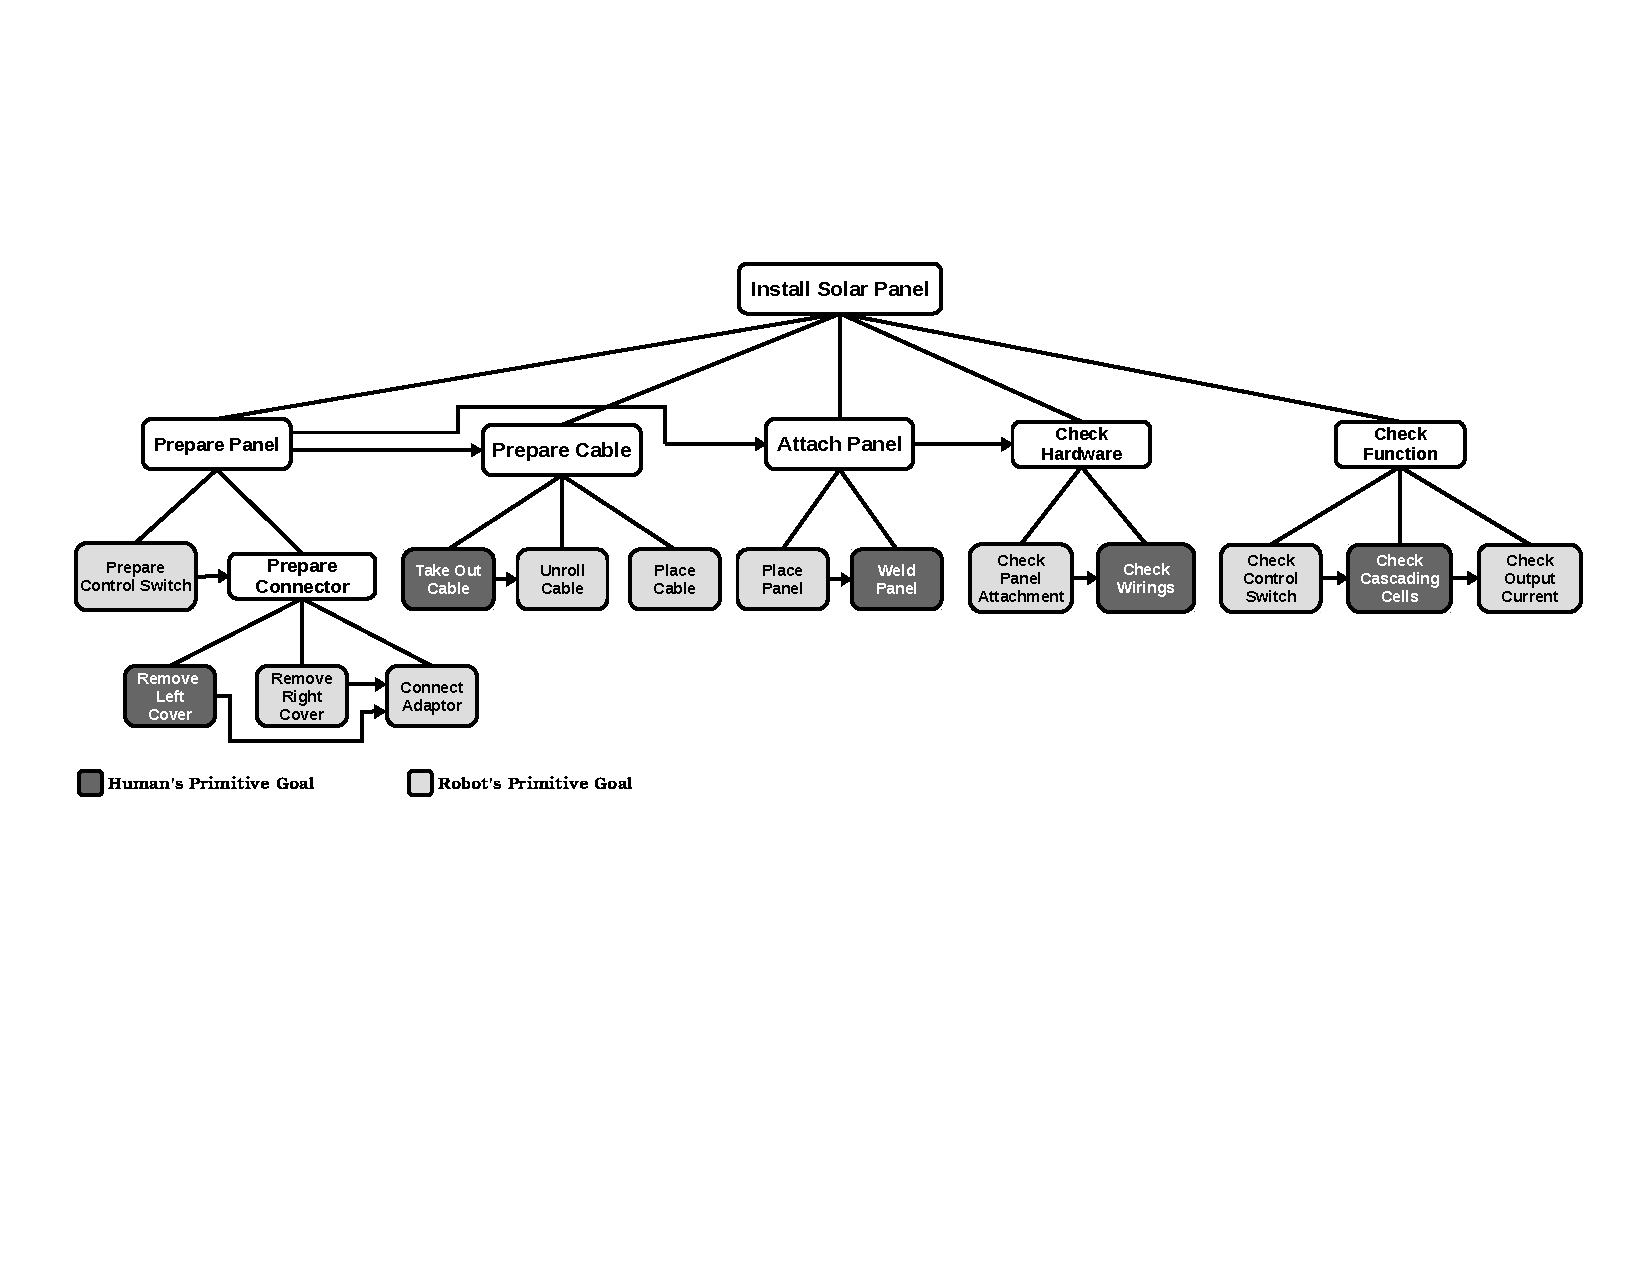
\includegraphics[width=1\textwidth]{figure/collaborationStructure.pdf}
  \caption{Collaboration structure used as the task model.}
  \label{fig:collaboration_structure}
\end{figure*}

\subsubsection{Framework}
\label{sec:theory}
The framework includes all of the mechanisms depicted as mental processes in
Figure \ref{fig:framework} along with the mental states. The mental
states shown in Figure \ref{fig:framework} comprise the knowledge base required
for all of the mechanisms in the overall model. The details about these mental
processes and mental states are described in Chapters \ref{ch:amct} and
\ref{ch:appraisals}. In this user-study, the Collaboration mechanism uses a
hierarchy of goals associated with tasks in the hierarchical task network
structure depicted in Figure \ref{fig:collaboration_structure}.

\subsubsection{The Robot}

We conducted our experiment with a KUKA Youbot (see Figure
\ref{fig:environment}). The robot was stationary on top of a desk and was able
to pick up and place available pegs corresponding to the robot's task. The robot
was operated based on Robot Operating System (ROS -- indigo) and was receiving
commands through the ROS-bridge from our Affective Motivational Collaboration
framework (see Figure \ref{fig:framework}). We provided a simple GUI using a
touch-screen monitor (see Figure \ref{fig:gui}) to a) express the robot's
positive, negative or neutral emotion through an emoticon, b) display the
robot's utterances, c) control turn-taking process of the collaboration, and d)
let the participants express (report) their positive, negative or neutral
emotion for each turn. The robot used the MaryTTS\footnote{http://mary.dfki.de/}
text-to-speech platform to provide corresponding speech for its utterances in
English.

\subsubsection{Robot Controller}
The robot controller is comprised of two major components: 1) ROS-bridge and 2)
joint controller (see Figure \ref{fig:framework}).
ROS-bridge\footnote{http://wiki.ros.org/rosbridge\_suite} provides an API to ROS
functionality for non-ROS programs which enables us to send action commands from
our framework (implemented in JAVA) to the robot's joint controller. The joint
controller receives action commands and translates them into actual joint and
actuator commands and sends them to the robot (see Figure \ref{fig:environment}).

\subsection{Experimental Design}

Our scenario was based on a table top turn-taking game that we designed to
simulate the installation of a solar panel. Participants collaborated one-on-one
with our robot to complete all the given tasks required to install the solar
panel. Each participant worked with the robot in two conditions, in a within
subject study. Each primitive task consisted of picking up and placing pegs on
predefined spots on the board (see Figure \ref{fig:game_board}). Each
pick-and-place was associated with the robot's or the participant's task. The
robot and the participants had their own unique primitive tasks that they had to
accomplish in their own turns. The final goal of installing a solar panel
required the robot and the participants to accomplish their own individual
tasks. Failure of any task could create an impasse during the collaboration.

\begin{figure}[tbh]
  \centering
  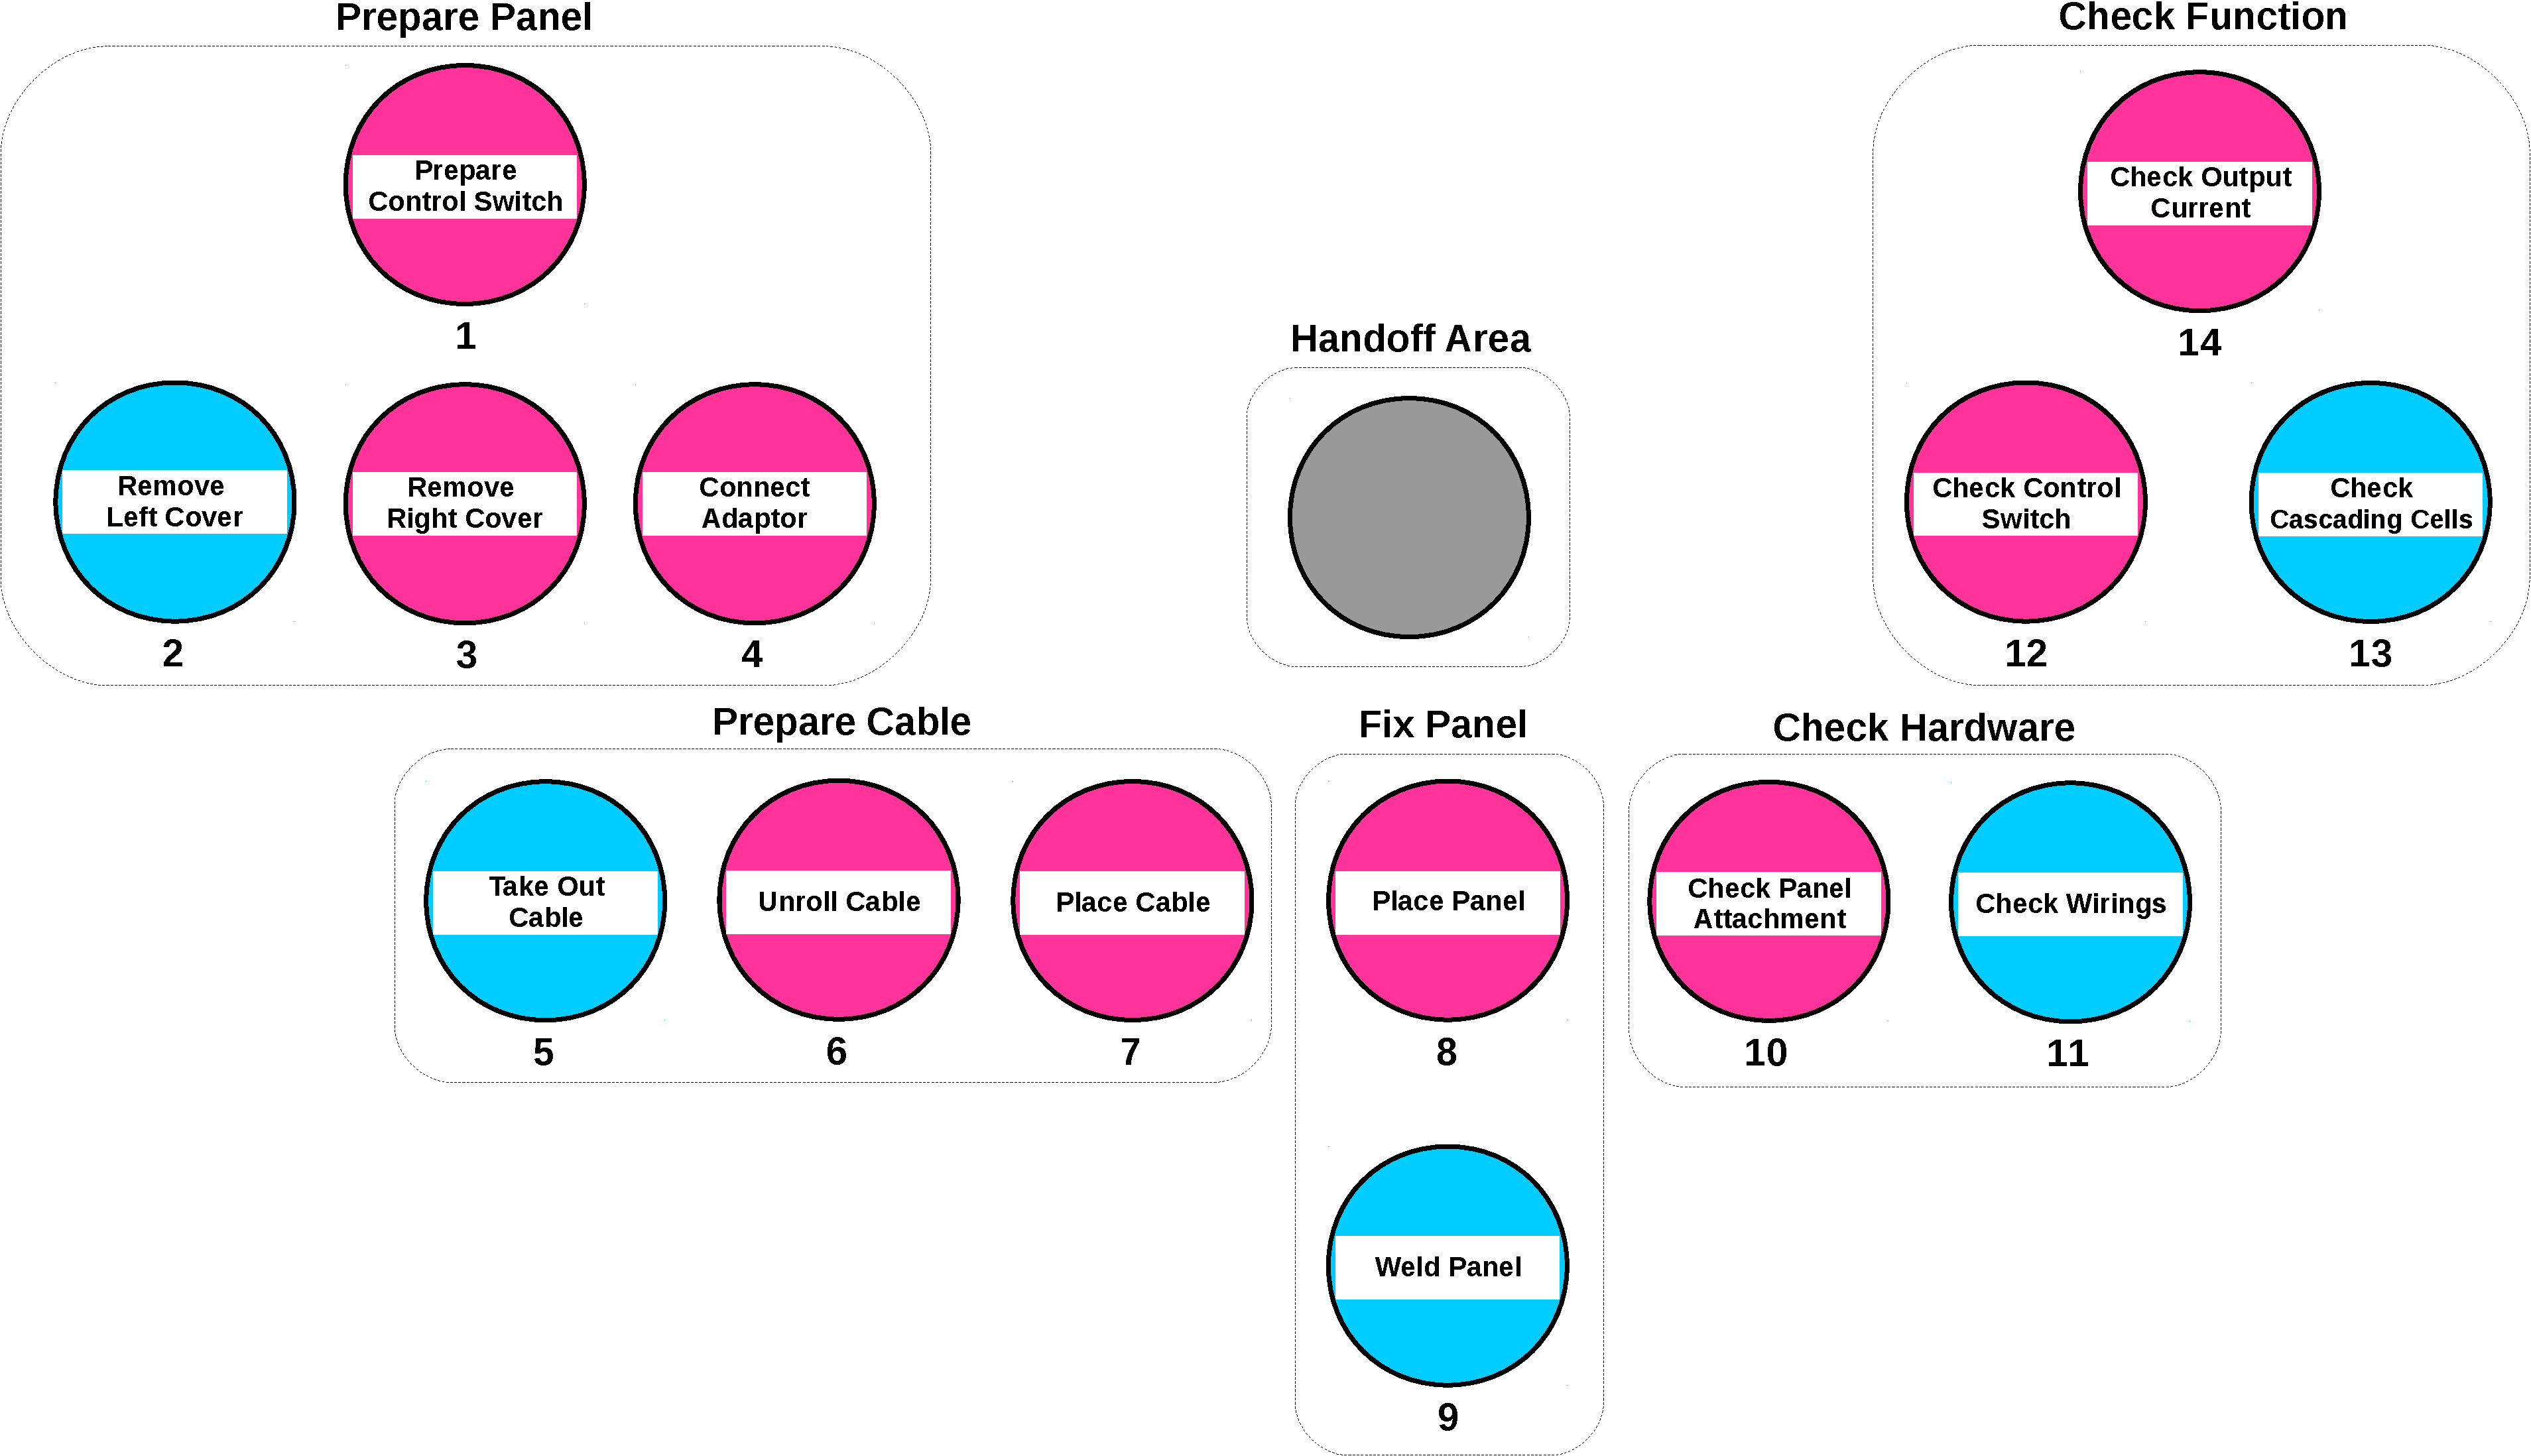
\includegraphics[width=1\textwidth]{figure/gameBoard.pdf}
  \caption{The layout of the available spots for the human and the robot to
  place their pegs during the collaboration.}
  \label{fig:game_board}
\end{figure}



\begin{figure}
\centering
\begin{subfigure}{.5\textwidth}
  \centering
  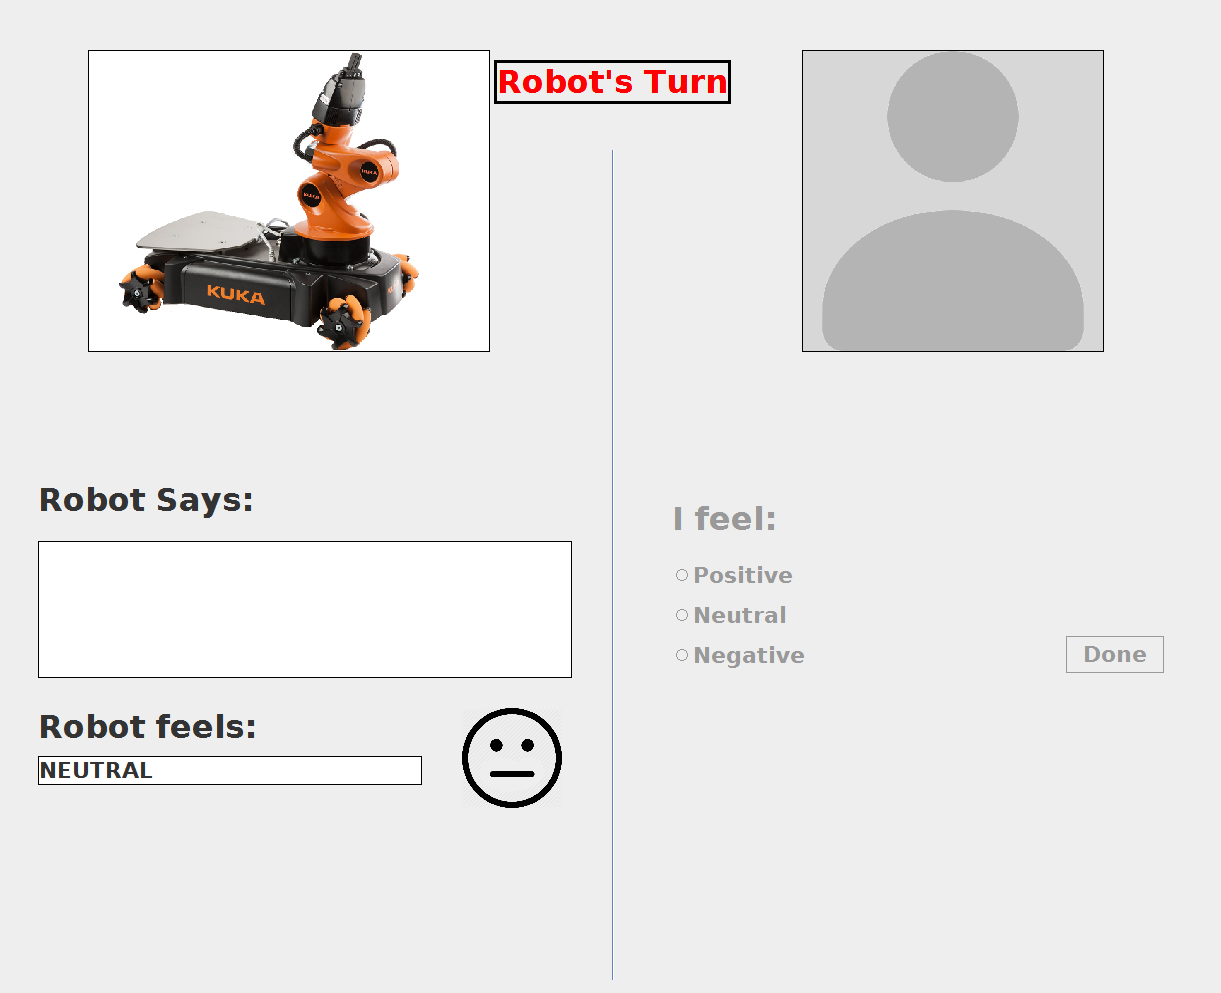
\includegraphics[width=.95\linewidth]{figure/robot-turn-gui.png}
  \label{fig:gui-robot}
\end{subfigure}%
\begin{subfigure}{.5\textwidth}
  \centering
  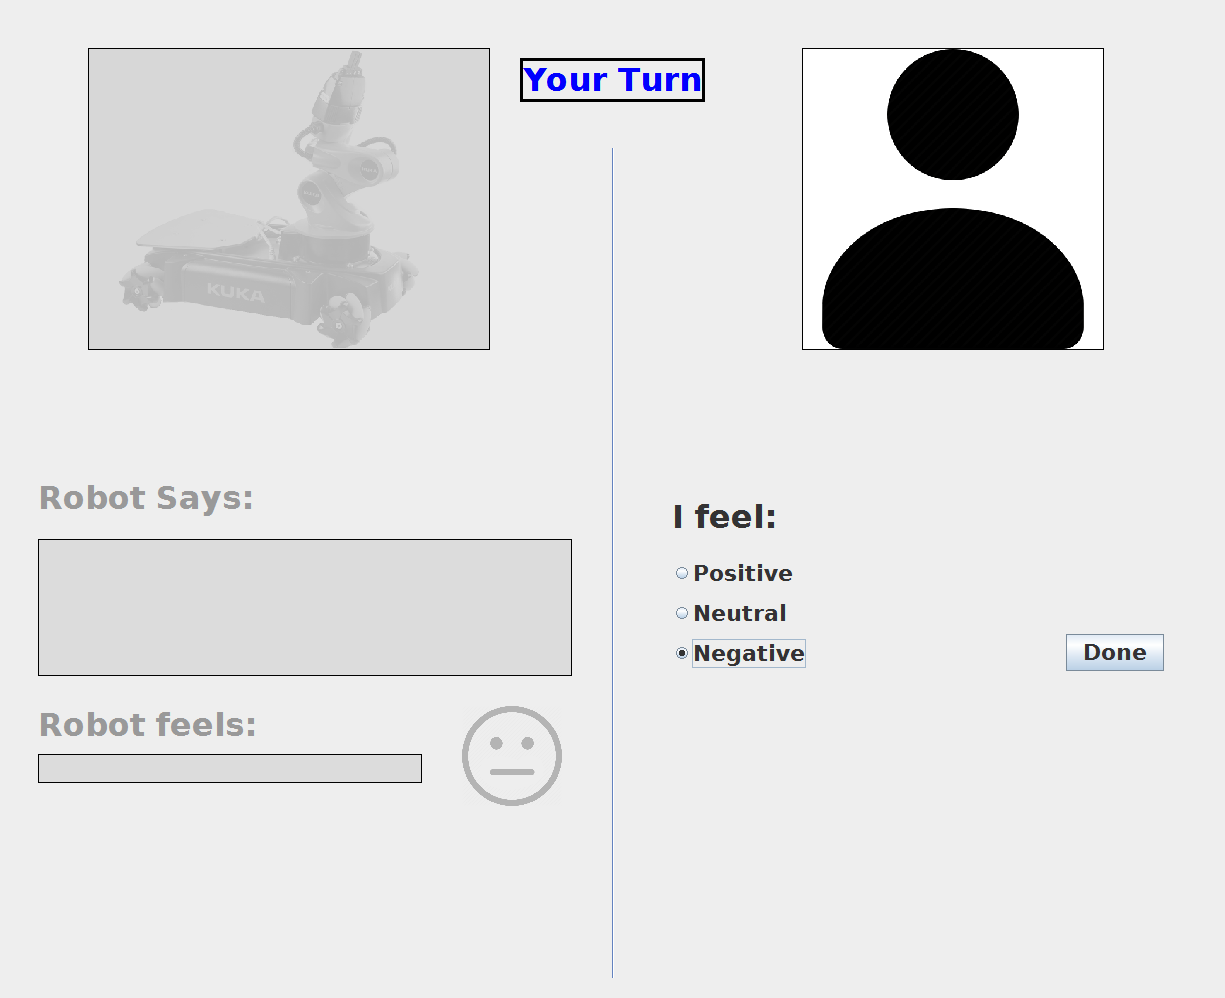
\includegraphics[width=.95\linewidth]{figure/human-turn-gui.png}
  \label{fig:gui-human}
\end{subfigure}
\caption{The Graphical User Interface (GUI) used during interaction.}
\label{fig:gui}
\end{figure}

\subsubsection{Interaction Paradigms}
\label{sec-interaction-paradigms}
At the beginning of each collaboration the robot asked each participant to
achieve the overall shared goal, i.e., ``installing the solar panel''. Then,
before working towards a new goal, the robot informed the participant about the
higher level nonprimitive goal (e.g. Prepare Panel -- see Figure
\ref{fig:collaboration_structure}) of which the primitives were going to be
working towards. The same procedure was used by the robot if there was a
decision to switch to another nonprimitive due to the failure of a task in
achieving the current goal. After achieving a new primitive goal, the robot
either informed the human that it would pursue the next goal, or it informed and
passed the turn to the human to execute the next task with respect to the
human's goal. In case of the human's turn, the robot waited for the human to do
a task, then the wizard let the robot know whether the human's goal was achieved
or not. Afterwards the robot made a decision about which goal to pursue and
informed the human accordingly. There were two conditions of the robot: 1)
emotion-aware and 2) emotion ignorant. The same procedure was applied to both
conditions.

The robot interacted via a) speech, b) the corresponding utterance on the
screen, c) negative, positive and neutral expression of emotion through an
emoticon on the screen. The robot used only neutral expression in the case of
emotion-ignorance. The interaction was controlled autonomously by the framework
we discussed in Section \ref{sec:theory} in both the emotion-ignorant and the
emotion-aware cases. The reasoning about which task should be done and
controlling the robot was entirely autonomous. Only the perception of the task
failure or achievement by the robot or by the participant was done by a wizard
monitoring the collaboration outside of the test area. The interaction was
structured based on the same collaboration structure (see Figure
\ref{fig:collaboration_structure}) for both conditions. The robot used the same
utterances in both conditions. In the emotion-aware condition the robot used a
different behavior in comparison with the emotion-ignorant condition only if the
participant was expressing a negative emotion in the event of a failure; i.e.,
the robot's utterances were identical in emotion-ignorant and emotion-aware
cases if in the latter the participant reported (expressed) a positive or a
neutral emotion.

Three different behaviors could be generated only in the emotion-aware
condition as a result of the Coping mechanism (planning, active coping, seeking
social support for instrumental reasons, and mental disengagement coping
strategies were involved to generate these three behaviors). These three
behaviors were 1) mitigating the human's negative emotion and postponing its own
task to help the human, 2) goal-management to switch to another goal which had
lower cost with respect to the human's negative emotion, and 3) task delegation
to the human to overcome the impasse. In each run, the human had two
predetermined task failures, and the robot had one. If the human expressed
negative emotion after the first human task failure, the robot responded by
mitigating the human's negative emotion by saying  ``It was not your fault. I
can help you with this task" and helping the human by providing a peg to fulfill
the human's task. If the human expressed negative emotion after the second human
task failure, the robot informed the human that they could proceed with another
task to save time while simultaneously requesting a new peg (i.e., help) from
the supervisor. If the human expressed negative emotion as a result of the
robot's task failure, the robot requested help from the human (who had the
correct peg). In the event that the human expressed positive or neutral emotion
during these three failures, the robot behaved identically in the
emotion-ignorant and the emotion-aware cases, by asking the supervisor for help.

\begin{figure}
  \centering
  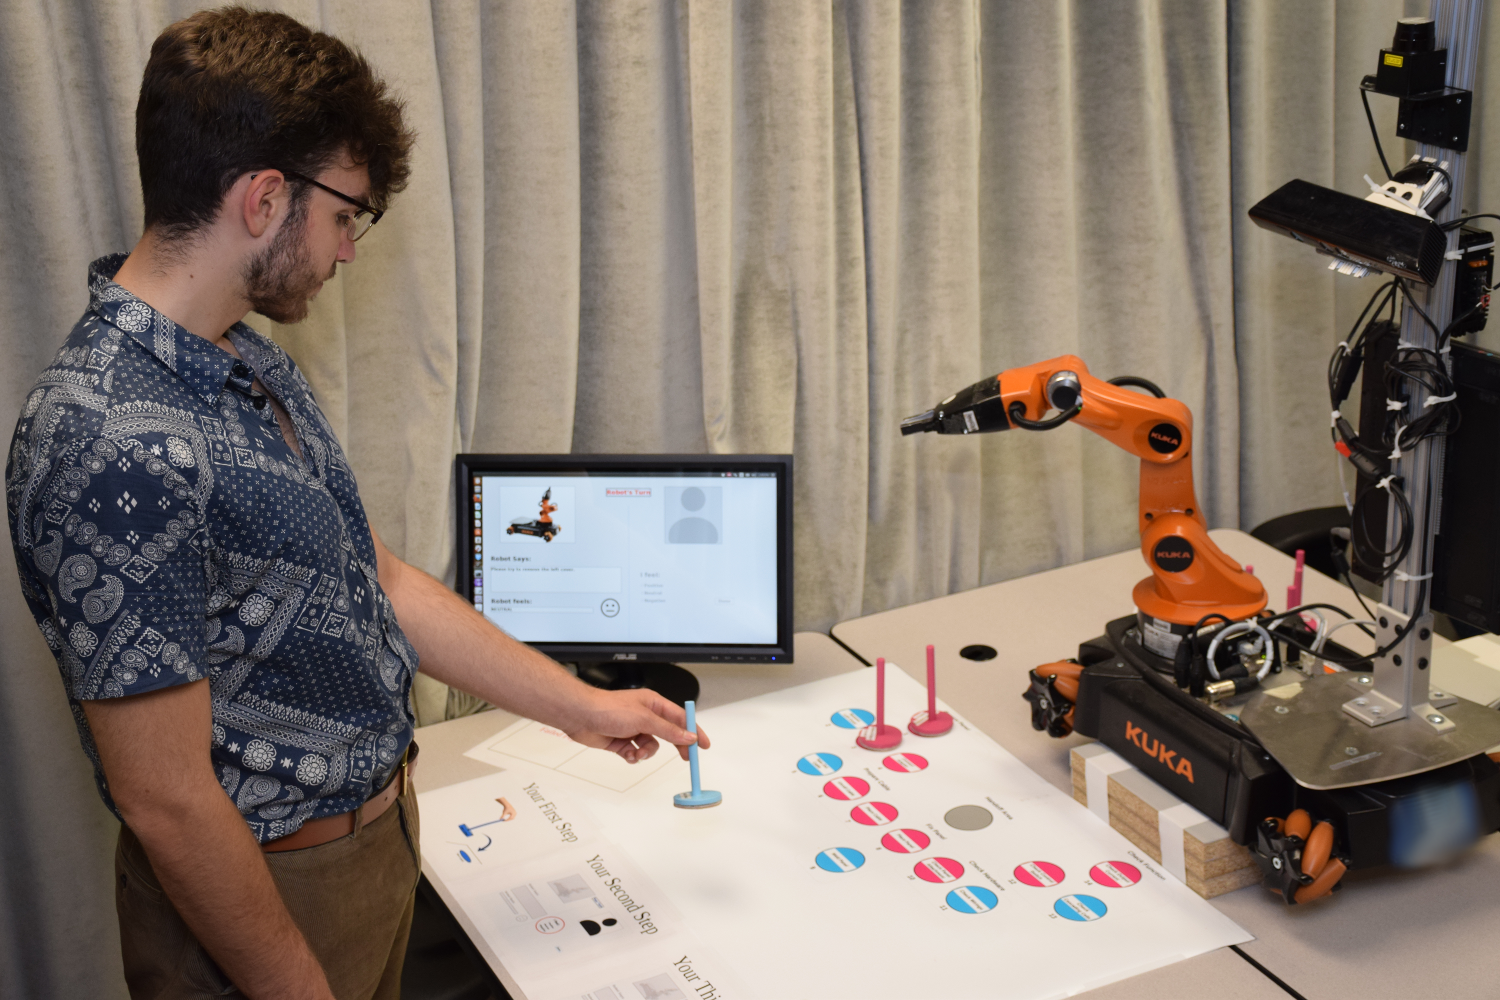
\includegraphics[width=0.9\textwidth]{figure/environment.png}
  \caption{Experimental setup.}
  \label{fig:environment}
\end{figure}

\subsection{Hypotheses}
\label{sec:hypotheses}
The non/social functions of emotions impact a collaboration process. Human
collaborators prefer to collaborate with others whose behaviors are influenced
by these functions of emotions depending on the context. We developed seven
specific hypotheses regarding the positive influence of emotion-awareness and
the usefulness of emotion function during collaboration:

\textit{\textbf{Hypothesis 1.}} Participants will feel closer to the emotion-aware
robot rather than the emotion-ignorant robot.

\textit{\textbf{Hypothesis 2.}} Participants will find the emotion-aware robot to be
more trustworthy than the emotion-ignorant robot.

\textit{\textbf{Hypothesis 3.}} Participants will find the emotion-aware robot to
have better performance in collaboration than the emotion-ignorant robot.

\textit{\textbf{Hypothesis 4.}} Participants will find the emotion-aware robot to be
more understanding of their feelings than the emotion-ignorant robot.

\textit{\textbf{Hypothesis 5.}} Participants will find the emotion-aware robot to be
more understanding of their goals than the emotion-ignorant robot.

\textit{\textbf{Hypothesis 6.}} Participants will feel more satisfied about the
collaboration when working with the emotion-aware robot rather than
emotion-ignorant robot.

\textit{\textbf{Hypothesis 7.}} Participants will perceive higher level of mutual
satisfaction with the emotion-aware robot than emotion-ignorant robot.

\subsection{Procedure}
\label{sec:procedure}
Participants were first given a brief description of the purpose of the
experiment. After the short introduction, they were asked to review and sign a
consent form. Participants were then provided with a written instruction of
their task and the rules for collaborating with the robot. Then, one of the
experimenters lead them into the experiment room and asked the participants
to asked to answer pre-experiment questionnaires. Afterwards, the experimenter
went through all the details of the instructions with the participants
standing in front of the collaboration board and the robot. The experimenter
confirmed participants' correct understanding of the tasks and informed them
of the types of task failures (i.e., fallen peg) that might occur during the
collaboration. Participants were told that researchers were developing a
collaborative robot and would like their help in evaluating their design.
Participants were provided with identical instructions and randomly assigned to
complete either the emotion-aware or the emotion ignorant condition first. They
were told that, after their collaboration with the robot, they would be asked to
answer a questionnaire on their experience. After completing the first round of
collaboration, participants answered a post-experiment questionnaire that
measured their perceptions of the robot, the task, and the collaboration
procedure. After answering the first post-experiment questionnaire, participants
were told that they were going to collaborate with the robot one more time and
the robot might not necessarily have the same collaborative behavior. After
completing the second round of collaboration, participants were asked to answer
the second post-experiment questionnaire which consisted of the same questions
as the first post-experiment questionnaire. Finally, participants were asked
to answer an open-ended questionnaire which measured their perception of
difference between two runs, their preference of collaborative robot between two
runs, and their reasons of preference.

\subsubsection{Measurements}
\label{sec:Measurements}
In our study two basic conditions of the robot were tested: a) the
emotion-ignorant condition, b) the emotion-aware condition. We measured
participants' recall of the collaborative behaviors presented by the robot using
an open-ended post-experiment questionnaire. We also specifically asked the
participants what behavior of the robot they liked during their collaboration.
We also evaluated participants' levels of satisfaction, trust, goal achievement,
mutual understanding of goals, mutual understanding of feelings, mutual
agreement, and also participants' beliefs about the efficiency of collaboration
and their feeling of robot's collaborative behaviors. Seven-point Likert scales
were used in these questionnaire items.

\subsubsection{Participants}
\label{sec:Participants}
A total of 37 participants participated in the experiment in 74 trials.
Participants were recruited from Worcester Polytechnic Institute's students and
staff as well as other people recruited from outside of the campus. The ages
of the participants varied between 19 and 74 with an average of 34.2 years
before our screening of 4 participants based on our sanity check questions. After
this screening, the ages of the participants varied between 19 and 54 with an
average of 30.8 years old. Of the 33 participants, 21 were female and 12
were male. Each participant participated in 2 trials. In one trial the robot was
aware of human's emotion and in the second trial the robot was ignoring human's
emotion. The order of these two trials were randomly assigned to each
participant. Overall, we used emotion-ignorant robot first in 16 experiments,
and emotion-aware robot first in 17 experiments.

\subsection{Results}

As discussed in Section \ref{sec:Measurements}, results of the user study were
gathered through a 31-question Likert-scale survey that was given to each
participant after each run with the robot, and through a 5-question open-ended
summary questionnaire at the end of the experiment.

\subsubsection{7-Point Likert Scale Survey Results}
As mentioned previously, the 7-point Likert scale survey was administered at
the end of the emotion-ignorant run and at the end of the emotion-aware run for
each participant. The 31 questions are generally categorized in accordance
with the seven hypotheses listed in Section \ref{sec:hypotheses} to evaluate the
humans' perceptions of the following seven categories, with 3-7 questions per
group: (1) the likability of the robot (2) the level of trust the human feels in
the robot (3) the human's perception of the robot's performance (4) the human's
perception of the robot's understanding of human's emotions (5) the human's
perception of the robot's understanding of human's and collaboration's goals and
objectives (6) the human's feeling about the collaboration and (7) the human's
perception of the human's and robot's mutual satisfaction with each other as
collaborative partners. The questions presented are provided in Table
\ref{fig:31questions-table}.

\begin{table}
 \centering
 \caption{The 31 Likert scale questions organized according to their
 categories (hypotheses).}
 \label{fig:31questions-table}
 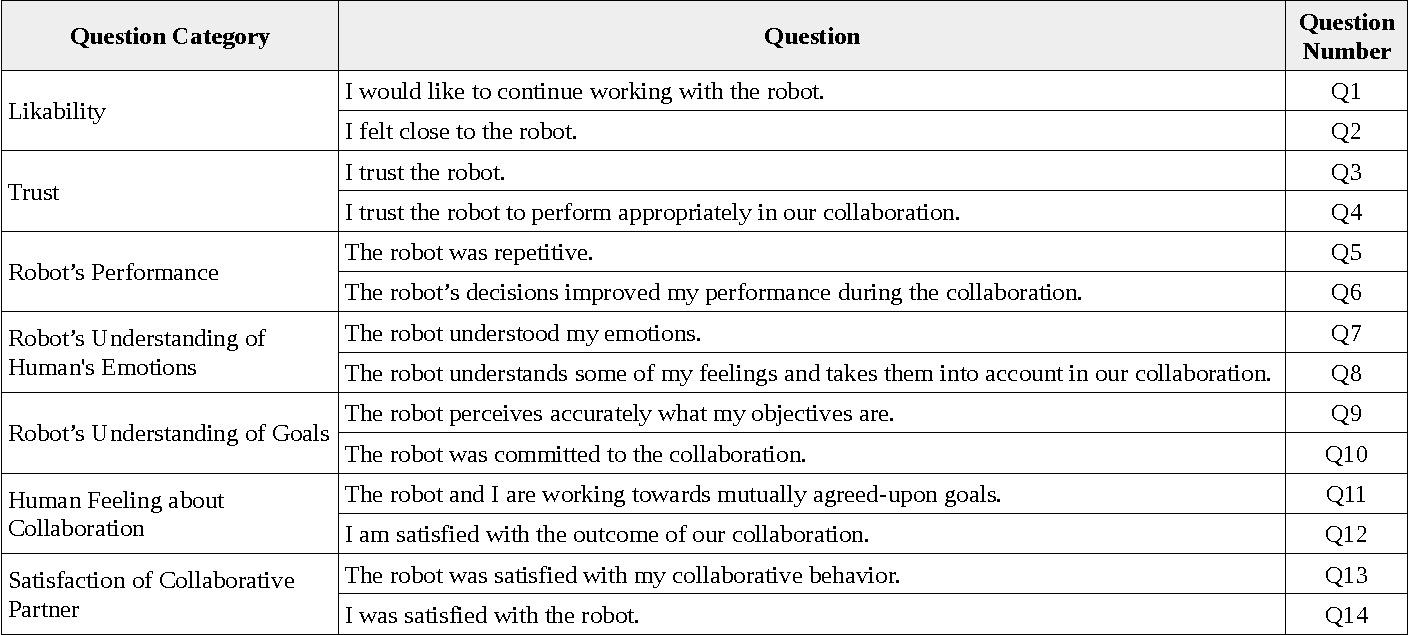
\includegraphics[width=1\textwidth]{figure/table1-croped.pdf}
\end{table}
\clearpage

The results were analyzed using a two-tailed paired t-test to analyze the
difference of means between the emotion ignorant and the emotion-aware
condition. Refer to Figures \ref{fig:overall-performance} -
\ref{fig:overall-satisfaction} for the results. Analysis of the results revealed
no statistically significant difference or consistent pattern based on which
condition the participant completed first.

\begin{figure*}[ht]
 \centering
 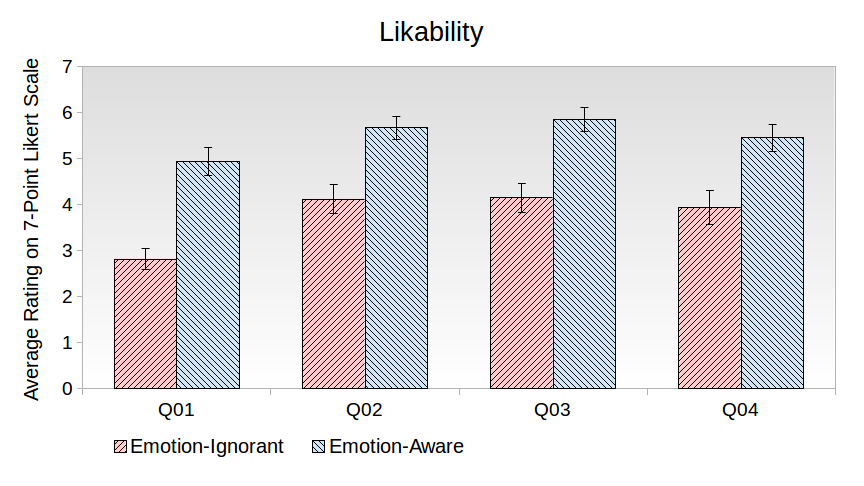
\includegraphics[width=0.8\textwidth]{figure/Overall-Likability.png}
 \vspace*{-5mm}
 \caption{Results of the Likert scale survey for Likability questions. The
 p-value for the difference between means is $\ll$0.001 for all questions.}
 \label{fig:overall-likability}
\end{figure*}

\hspace*{-8mm} \textbf{Likability of the Robot}
\label{sec:Likability}
\\Questions 1 through 4 addressed the likability of the robot. As shown in
Figure \ref{fig:overall-likability}, participants rated the emotion-aware robot
1.5-2.1 points higher than the emotion-ignorant robot. These results
indicate that participants felt closer with and preferred working with the
emotion-aware robot; these results support Hypothesis 1, which stated that
humans would prefer to work with the emotion-aware robot over the
emotion-ignorant robot. \\

\hspace*{-8mm} \textbf{Human Trust in the Robot}
\label{sec:Trust}
\\ Questions 5-9 were designed to measure the degree of trust that the human
participants felt in the robot. As shown in Figure \ref{fig:overall-trust},
participants trusted the emotion-aware robot, on average, a minimum of 1.4
points more than the emotion-ignorant robot, both in general and in terms of
collaboration performance. In Question 5, participants rated a
general statement of trust 1.5 points higher in the emotion-aware
case. Additionally, in Question 7, participants rated their trust in the
emotion-aware robot to perform appropriately during collaboration an average of
5.9 on a 7-point Likert scale, where 7.0 would indicate maximum trust; this
indicates an acceptable level of trust in the robot's collaborative
abilities. These results support Hypothesis 2, that posits that human
participants would find the emotion-aware robot to be more trustworthy than the
emotion-ignorant robot.\\

\begin{figure*}[h]
\centering
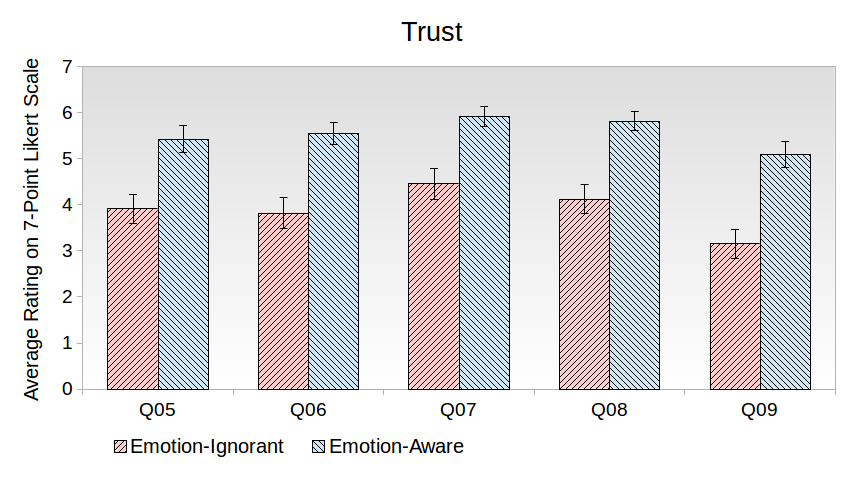
\includegraphics[width=0.8\textwidth]{figure/Overall-Trust.png}
\caption{Results of the Likert scale survey for questions related to trust. The
p-value for the difference between means is $\ll$0.001 for all questions.}
\label{fig:overall-trust}
\end{figure*}

\begin{figure*}[h]
\centering
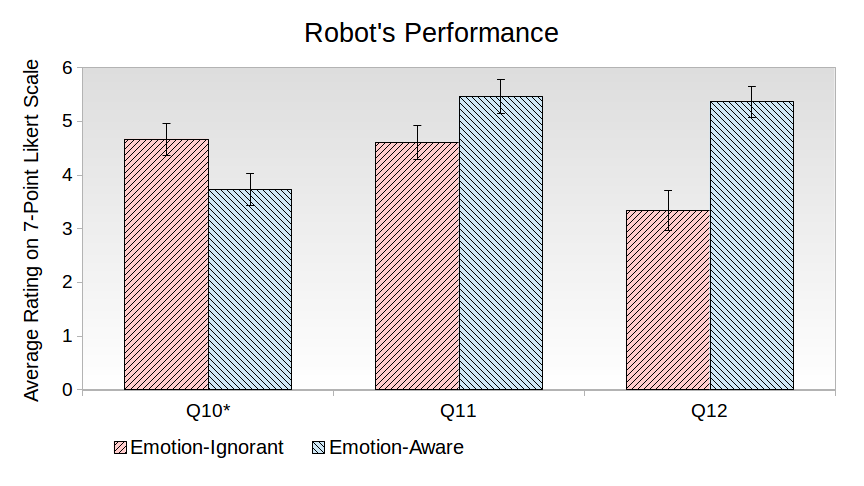
\includegraphics[width=0.8\textwidth]{figure/Overall-Performance.png}
\vspace*{-5mm}
\caption{Results of the Likert scale survey for questions related to the robot's
performance. The p-value for the difference between the means for questions 10,
11 and 12 are 0.001, 0.063 and $\ll$0.001, respectively.}
\label{fig:overall-performance}
\end{figure*}

\hspace*{-8mm} \textbf{Perception of the Robot's Performance} 
\label{sec:Performance}
\\Question 10 (which is reverse-scored) measures the participant's perception of
repetitiveness in the robot during the collaboration. In both conditions,
participants rated the robot as moderately repetitive, with the emotion-ignorant
robot's average response being about 1.1 points higher than the emotion-aware.
This result correlates with several of the open-ended responses which described
the emotion-aware robot's behaviors as ``cute'' and ``interesting'', refer to
Section \ref{sec:Open-Ended}. Question 11, which asks about the efficiency of
the robot's decisions is the only question of the 31 questions that did not have
a statistically significant difference between the emotion-aware and the
emotion-ignorant case. This correlates with the result of the open-ended
question asking which condition of the robot exhibited behaviors that could
prevent human error (refer to \ref{sec:Open-Ended}); in response to this
question, several respondents stated that it may be quicker or simpler to call
the supervisor in the event of a task failure, rather than changing the order of
the tasks. According to the results from Question 12, the participants felt that
the emotion-aware robot's decisions during collaboration improved their own
performance, with an average rating of 5.4, while the emotion-ignorant robot
only received an average rating of 3.3, indicating that participants felt it was
not able to interact in such a way as to increase the human's performance; refer
to results from Question 6. These results support Hypothesis 3, which posited
that humans will perceive the emotion-aware robot as being more capable than the
emotion-ignorant robot. \\

\hspace*{-8mm} \textbf{Robot's Understanding of Human Emotions} 
\label{sec:Emotions}
\\In Questions 13 through 17, participants evaluate the robot's understanding of
humans' emotions. In questions 13, 15, and 16, participants rated the
emotion-aware robot, on average, a minimum of 1.8 points higher than the
emotion-ignorant robot. In response to questions 14 and 17, which are
reverse-scored, participants ranked the emotion-ignorant robot 1.2 and 2.0
points higher, respectively, than then emotion-aware robot. The results
of all five questions in this category support Hypothesis 4. \\

\begin{figure*}[tbh]
\centering
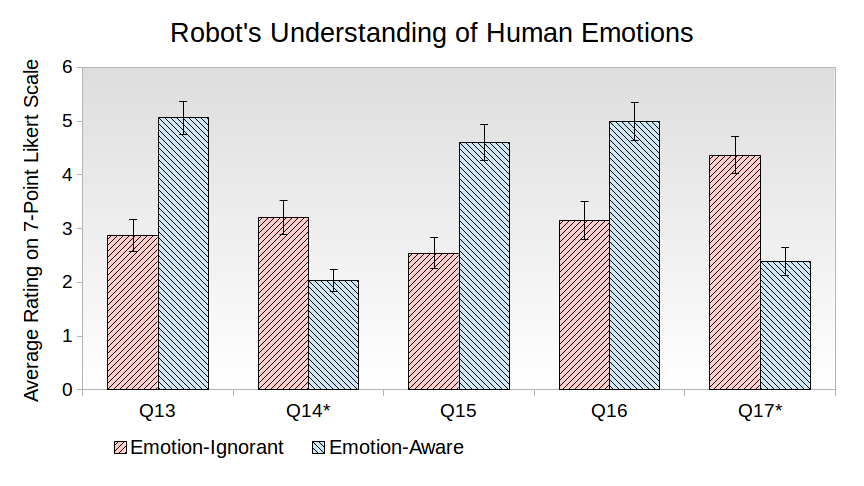
\includegraphics[width=0.8\textwidth]{figure/Overall-Emotions.png}
\vspace*{-5mm}
\caption{Results of the Likert scale survey for the questions related to the
robot's understanding of human emotions. The p-value for the difference between
the means is $\ll$0.001 for all of the questions except Question 14, for which
the p-value is 0.003.}
\label{fig:overall-emotions}
\end{figure*}

\hspace*{-8mm} \textbf{Robot's Understanding of Human and Collaboration Goals}
\label{sec:Goals}
\\Questions 18 and 19 were reverse-scored questions intended to determine
whether the humans felt that the robot understood the shared collaboration goal and the
human's personal goal, respectively. For both conditions of the robot, the
average scores were lower than 3.5, indicating that the human's perceived the
robot as having some understanding of the goals. For both questions, the
emotion-ignorant robot's average score was significantly higher than the
emotion-aware robot's score. Similarly, Question 20 was a measure of whether the
human perceived that the robot correctly perceived the human's goal.
On average, participants provided an average rating for the emotion-aware robot
that was 1.5 points higher than that for the emotion-ignorant robot. Question 21
measured the human perception of the robot's commitment to the collaboration;
for this measure, the average participant score assigned to the emotion-aware
robot was 6.2 points out of a maximum of 7 points, indicating that the
participants felt that the emotion-aware robot was strongly committed to the
collaboration. The emotion-ignorant robot received an average rating of 4.4
points, indicating only moderate commitment. These results strongly support
Hypothesis 5, which posits that humans will feel that the emotion-aware robot
will better understand their goals than the emotion-ignorant robot.\\

\begin{figure*}
\centering
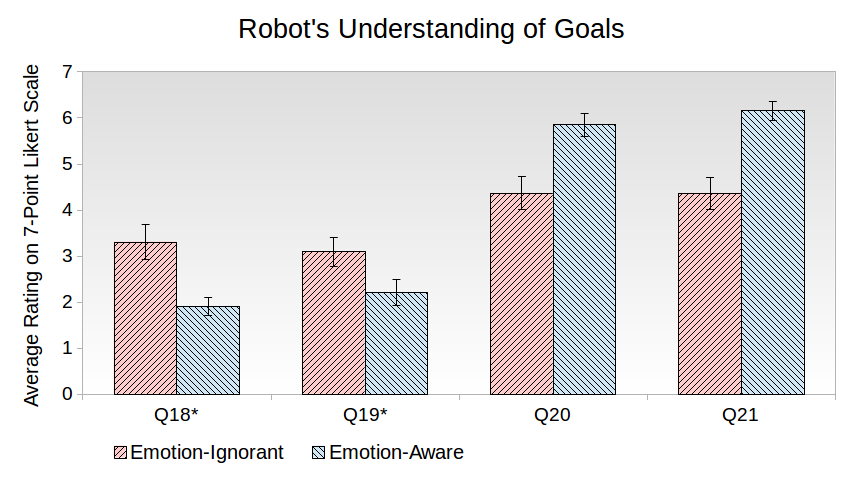
\includegraphics[width=0.8\textwidth]{figure/Overall-Goals.png}
\caption{Results of the Likert scale survey for questions related to the robot's
understanding of goals. The p-value for the difference between the means for all
questions is $\ll$0.001, except Question 19, for which the p-value is 0.006.}
\label{fig:overall-goals}
\end{figure*}

\begin{figure*}
\centering
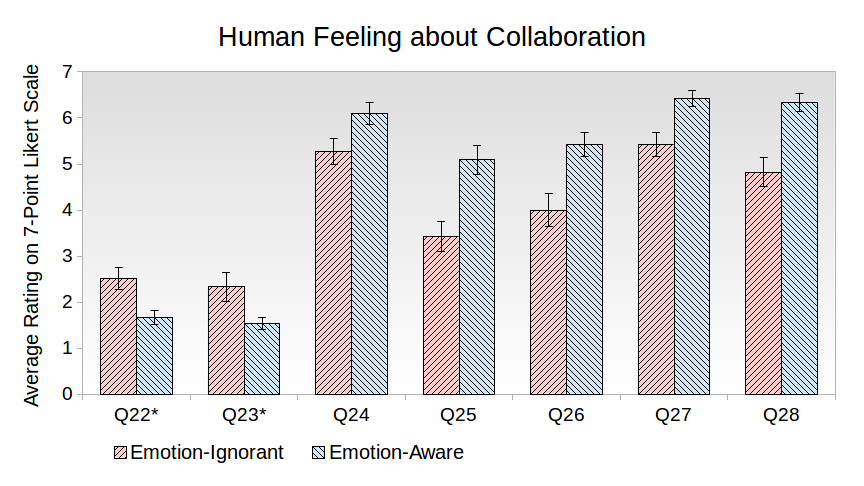
\includegraphics[width=0.8\textwidth]{figure/Overall-Collaboration.png}
\caption{Results of the Likert scale survey for questions related to the human's
feeling about the collaboration. The p-value for the difference between the
means is $\ll$0.001 for questions 22, 25, 26, and 28. The p-value for Questions
23, 24 and 27 are 0.02, 0.008 and 0.001, respectively.}
\label{fig:overall-collaboration}
\end{figure*}

\hspace*{-8mm} \textbf{Human's Feeling about the Collaboration}
\label{sec:Collaboration}
\\Questions 22 through 28 were designed to gauge how the human participants
felt about the partnership within the collaboration and the outcome of the
collaboration. For each of the 7 questions, the participants ranked the
emotion-aware robot as better than the emotion-ignorant robot, by a minimum,
on average, of 0.8 points. Questions 24, 27 and 28 addressed whether the robot
and the participant were working toward mutually agreed-upon goals and on the
outcome of the collaboration; in the emotion-aware condition, participants rated
the robot a minimum of 6.1 points, on average, while rating the emotion-ignorant
robot 1-1.6 points lower, indicating that the participants felt a very strong
sense of collaboration with the emotion-aware robot, and only a moderate sense
of collaboration with the emotion-ignorant robot. Questions 25 and 26 address
whether the robot and the participant set the collaboration goals together;
these two questions have lower scores than Questions 24, 27 and 28, for both the
emotion-aware and the emotion-ignorant case. The lower overall scores are
likely due to the fact that the robot decides the task order or action in the
event of failure in both conditions; however, the higher score in the
emotion-aware case may indicate that emotional awareness can increase a feeling
of collaboration. These results support Hypothesis 6 that humans will feel
a greater sense of mutual collaboration and understanding about the
collaboration with the emotion-aware robot.\\

\hspace*{-8mm} \textbf{Human Perception of Mutual Satisfaction with
Collaborative Partner}
\label{sec:MutualSatisfaction}
\\ Questions 29, 30 and 31 were designed to measure the human's perception
of the robot's satisfaction with the human, the human's satisfaction with the
robot and the mutual understanding between the human and the robot,
respectively. The participants provided an average response in the emotion-aware
condition of 5.8, 5.9 and 5.7 to Questions 29, 30 and 31, respectively,
indicating a high level of mutual satisfaction; all three answers were
about 1.4-1.9 points lower, on average, in the emotion-ignorant condition. These
results indicate a higher level of satisfaction working with the robot in the
emotion-aware condition, and strongly support Hypothesis 7, which posited that
humans will feel a greater sense of mutual satisfaction with the emotion-aware
robot than the emotion-ignorant robot.

\begin{figure*}
\centering
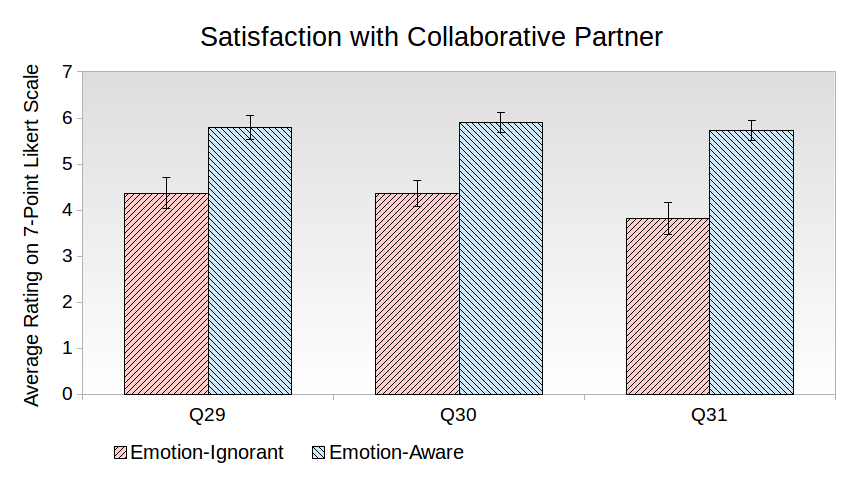
\includegraphics[width=0.8\textwidth]{figure/Overall-Satisfaction.png}
\caption{Results of the Likert scale survey for questions related to
satisfaction with collaborative partner. The p-value for the difference between
means is $\ll$0.001 for all questions.}
\label{fig:overall-satisfaction}
\end{figure*}

\subsubsection{Results from the Open-Ended Questionnaire} 
\label{sec:Open-Ended}
As described in Section \ref{sec:procedure}, each participant answered an
open-ended questionnaire at the end of the study. Table
\ref{fig:Open-Ended-Table} summarizes the questionnaire and which condition
users preferred for certain conditions (i.e. emotion-ignorant or emotion-aware).
Note that some users chose not to state a preference regarding which condition
they preferred for certain conditions; because we were specifically interested
in whether users preferred the emotion-aware case, we considered the ambiguous
responses to be failures in the binomial analysis. The binomial analysis is
based on a population size of 33. 

\begin{table}[tbh]
  \centering
  \caption{Open-ended questionnaire questions and results. (*Note: Because we
  are evaluating whether humans prefer an emotion-aware robot, these results are
  taken as negative test results when calculating the p-value using the binomial
  distribution. Only those participants who clearly indicated a preference for
  the emotion-aware robot are taken as positive test results.)}
  \label{fig:Open-Ended-Table}
  \vspace*{-3mm}
  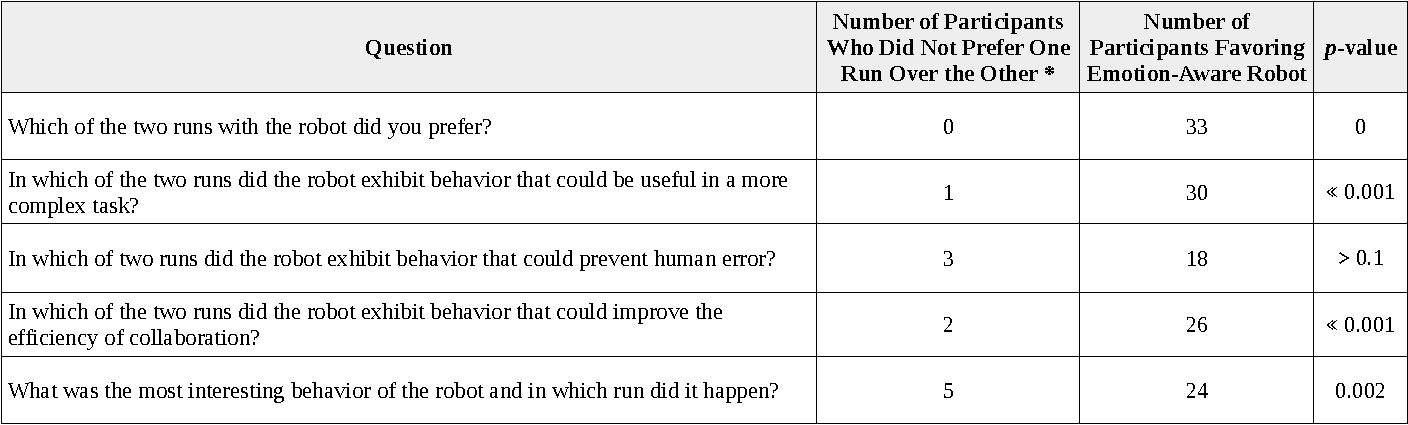
\includegraphics[width=1\textwidth]{figure/table2-croped.pdf}
\end{table}

As shown in Table \ref{fig:Open-Ended-Table}, 100\% of users unambiguously
preferred the run with the emotion-aware robot. In general, this preference
stemmed from a feeling of closeness and partnership, as seen in these responses:
``the robot had emotions and responded to my emotions. Also, ``what it said about
my failing was cute and aimed to make me feel better.'' Another example is ``I
liked feeling needed and accounted for; I felt closer to the robot.'' Finally,
``I saw the changes in its feeling, which motivated me to care more about my
act...I also liked that he asked me to correct its failure, although it could
ask the supervisor.''  

When asked in which of the two runs the robot exhibited behavior that could be
useful in a more complex task, 90.9\% chose the emotion-aware robot. In general,
respondents thought that the emotion-aware robot was better at problem solving,
more adaptable, and more capable of handling the social complexities that occur
in collaboration, as shown in responses such as ``The robot explained
motives...which is important to keep a team communicating and on the same
pace.'' Also, ``When we failed he initially switched to a new task and then came
back to the originally failed task. It kept me from getting irritated and
negative.'' Finally, ``The more complex, the more necessary it is to understand
how humans think and operate...an empathetic robot can adapt, encourage and
help.'' It is worth noting that one respondent preferred the emotion-ignorant
case, saying ``In a more complex task it might be better for the robot to take
control and simply tell me what to do; trying to be understanding and
collaborative wouldn't be as important as doing the task correctly.''

The only question that did not provide statistically significant support in
favor of the emotion-aware robot related to which case the robot exhibited
behavior that could prevent human error. About 36.4\% of respondents thought
that the emotion-ignorant robot was more likely to prevent human error; however, all
but one of these cited calling the supervisor as the main method of preventing
human error, in spite of the fact that the instructions indicated that the
robot's need to call the supervisor counted against the collaboration. Of the
54.5\% who thought that the emotion-aware robot was better at preventing human
error, most cited the robot's ability to console the human as the main behavior
that could prevent human error. Respondents indicated that this enabled them to
move on and feel better about the collaboration, as with this response: ``The
robot switched to a different task and we came back to an error later. This
allowed my mind to move away from being frustrated. I was able to complete a
different task which felt like a win - then come back and finish the error.
Making my mind move away from frustration could definitely prevent more
errors.''

When asked in which of the runs the robot exhibited behavior that could improve
the efficiency of the collaboration, 78.8\% responded with the emotion-aware
case; of these, the vast majority stated that this was because of the robot's
ability to change the order of tasks in the event of a failure, and to ask the
human for help.

Finally, when asked in which run the most interesting behavior occurred,
72.7\% chose the emotion-aware condition. Of these respondents, 12
individuals stated that the robot's attempt to console the human by saying ``It
was not your fault'' in response to the human's negative emotion that occurred
as a consequence of the human's failed task was the most interesting behavior,
and a majority mentioned that it actually made them feel more positive. Six
participants referred to the robot's ability to understand and express emotion.
Several participants referred to the robot's ability to communicate, including
the ability to ask questions. Of those who responded with the emotion-ignorant
case, most found the ability to call the supervisor, and mechanical functions,
such as gripping, to be most interesting.

\subsubsection{Impact of Demographics} 
As mentioned in Section \ref{sec:Participants}, we recorded the age and gender
of each participant. Although it was not the primary purpose of the study, we
investigated the Likert scale results to determine if there were any relevant
trends based on the demographics of the participants.

Age did reveal an interesting pattern. We divided the participants into two
groups, below 30 years of age and 30 or above. While question-by-question
comparisons revealed only a few statistically significant differences based on
age, a general pattern emerged. For all but four of the 31 questions presented,
the younger age group reported higher scores than the older age group (or lower,
in the case of reverse-scored questions)for the emotion-aware robot. In the
emotion-ignorant case, the younger group tends to score the robot nearer to
the same value as the older age group for all but seven questions, leading to a
pattern in which the score drop between the emotion-aware and the
emotion-ignorant case was more for the younger group than for the older group;
the seven questions that broke this pattern were 7, 9, 11, 12, 18, 19 and 22.

\begin{figure*}[tbh]
\centering
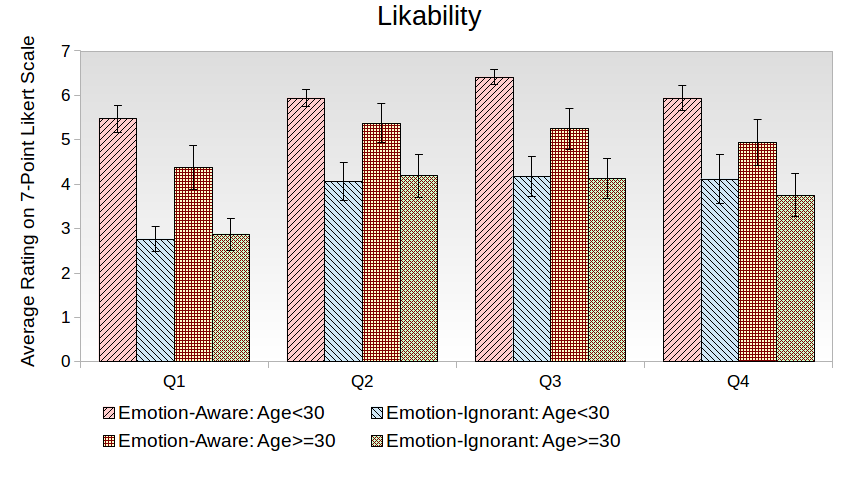
\includegraphics[width=0.9\textwidth]{figure/Age-Likability.png}
\caption{Impact of age on results of Likert scale questions related to
likability.}
\label{fig:age-likability}
\vspace*{15mm}
\end{figure*}

\begin{figure*}[!h]
\centering
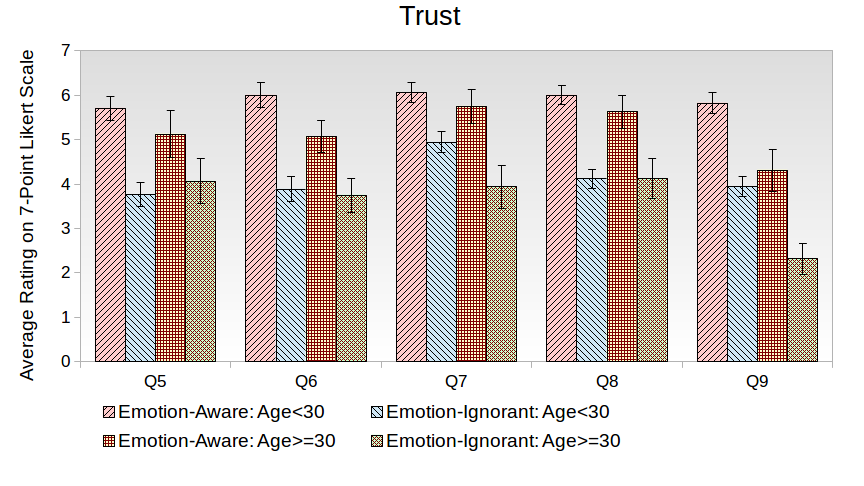
\includegraphics[width=0.9\textwidth]{figure/Age-Trust.png}
\caption{Impact of age on results of Likert scale questions related to trust.}
\label{fig:age-trust}
\vspace*{15mm}
\end{figure*}

\begin{figure*}[!h]
\centering
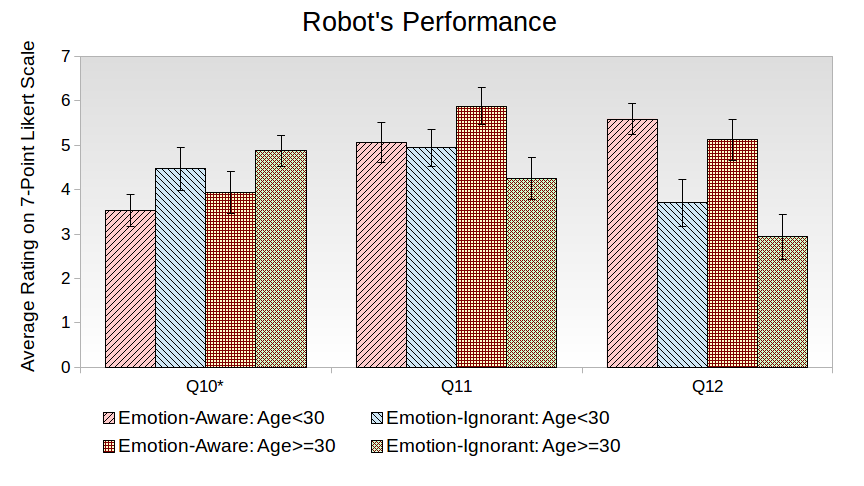
\includegraphics[width=0.9\textwidth]{figure/Age-Performance.png}
\caption{Impact of age on results of Likert scale questions related to
performance.}
\label{fig:age-performance}
\vspace*{15mm}
\end{figure*}

\begin{figure*}[!h]
\centering
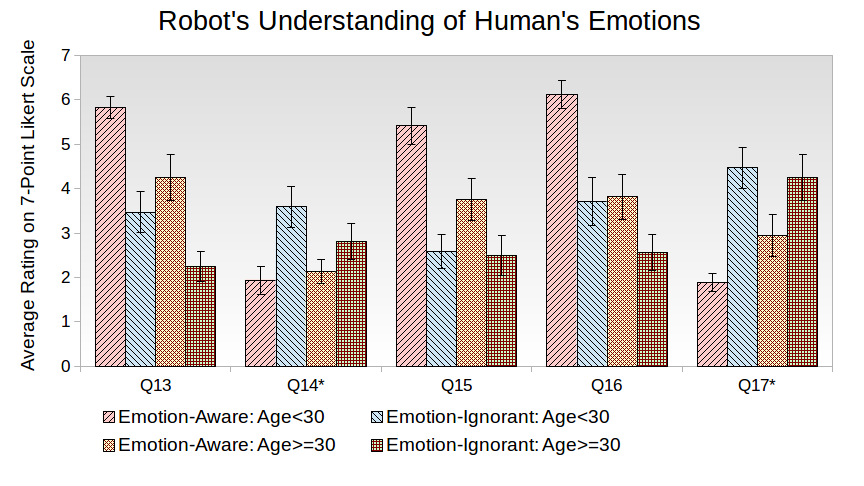
\includegraphics[width=0.9\textwidth]{figure/Age-Emotions.png}
\caption{Impact of age on results of Likert scale questions related to robot's
understanding of human's emotions.}
\label{fig:age-emotions}
\vspace*{15mm}
\end{figure*}

\begin{figure*}[!h]
\centering
\includegraphics[width=0.9\textwidth]{figure/Age-Goals.png}
\caption{Impact of age on results of Likert scale questions related to robot's
understanding of goals.}
\label{fig:age-goals}
\vspace*{10mm}
\end{figure*}

\begin{figure*}[!h]
\centering
\includegraphics[width=0.9\textwidth]{figure/Age-Collaboration.png}
\caption{Impact of age on results of Likert scale questions related to human's
feeling about collaboration.}
\label{fig:age-collaboration}
\vspace*{15mm}
\end{figure*}

\begin{figure*}[!h]
\centering
\includegraphics[width=0.9\textwidth]{figure/Age-Satisfaction.png}
\caption{Impact of age on results of Likert scale questions related to
satisfaction with collaborative partner.}
\label{fig:age-satisfaction}
\end{figure*}

\subsection{Discussion}
Based on the results, all participants prefer to work with the emotion-aware
robot. Humans find the emotion-aware robot more likable and more trustworthy, as
indicated in the Likert-scale responses and the open-ended questionnaire
responses. Based on the responses, the emotional interaction with the robot can
help create a sense of closeness and enjoyment that makes humans want to
continue working with the robot.

The results also indicate that the emotion aware robot can better maintain a
collaborative relationship. Both Likert-scale responses and Open-Ended
Questionnaire responses indicate this. Humans felt a stronger sense of the
robot's commitment to the collaboration, and greater understanding of their
goals and emotions from the robot. Several open-ended responses also indicated
that the robot was able to successfully motivate people and maintain their
commitment to the collaboration, especially when tasks failed. Additionally, as
shown in Section \ref{sec:Performance}, humans rated the emotion-aware case much
higher than the emotion-ignorant case when asked which robot's decisions
improved their performance, in essence acknowledging that their collaborator's
(i.e., the robot's) decisions had a significant impact on their performance. As
some of the open-ended responses indicated, successfully managing emotions
within the collaboration can help keep the collaboration on track, and prevent
distractions due to guilt and other negative emotions.

Finally, the emotion-aware robot developed a stronger sense of  partnership
through greater communication. The participants felt better understood by the
emotion-aware robot, and felt that the goals were more mutually agreed-upon,
refer to Section \ref{sec:Collaboration}. As evidenced in the following
response, the emotion-aware robot was successfully able to create a sense of
partnership through its more open communication style: ``Communication is very
important. In the first run (i.e. emotion-aware) the robot states what tasks he
is working on, it is clear and straight-forward. Also during the first run the
robot cares about the human(me)'s feelings and cheers me up when I failed at the
tasks, I think that could also improve efficiency of collaboration, because it
would be more like a team or partnership.''

\chapter{Conclusion}
\label{ch:conclusion}

\section{Discussion}
This thesis presents the Affective Motivational Collaboration (AMC) theory and
our computational framework. The AMC is built on the SharedPlans theory of
collaboration \cite{grosz:plans-discourse} and the cognitive appraisal theory of
emotions \cite{marsella:ema-process-model}
\cite{scherer:appraisal-processes}. Our motivation to develop AMC was the lack
of a theory describing the processes involved in a dyadic collaboration as well
as their relationship and influences on each other. In particular, in this
thesis we emphasized the reciprocal influence of the collaboration structure and
the appraisal processes in collaboration. We provided algorithms to compute
appraisal variables and their influence on collaboration processes, e.g., goal
management. In general, our contribution in this thesis was to provide a theory
which describes emotion-regulated goal-driven behaviors within a dyadic
collaboration. A further contribution of this thesis is to account for the
influence of motives on the coping processes in collaboration. We validated our
individual appraisal algorithms as well as our overall computational framework
by conducting an online crowd-sourcing user study and a laboratory emd-to-end
system user study, respectively. The first study investigated whether humans and
our appraisal algorithms provide similar answers to questions with respect to
factors involved in our appraisal algorithms. The second study investigated a)
the importance of emotional-awareness in collaboration, and b) the overall
functionality of the AMC framework to autonomously control interactions of a
collaborative robot.

After our introduction in Chapter \ref{ch:introduction}, we presented the
theoretical background on the two major foundations of our theory in Chapter
\ref{ch:background}. First, we reviewed the prominent computational
collaboration theories including SharedPlans and Joint Intentions. We focused on
the main concepts characterizing requirements of a collaboration introduced by
these theories. We also analyzed the similarities and differences between these
theories in terms of their essential concepts as well as their theoretical and
practical applications. These applications involved the fields of robotic and
artificial agents. Then, we continued discussing what emotions are and more
importantly how they can influence one's cognition and social life. We also
discussed the role of emotions in communicating one's internal states to others
as the basic rationale behind different social emotions. We confined our
discussion about emotion to artificial emotions in social robots or agents.
Third, we reviewed existing computational models of emotions, including
appraisal theory, analyzing their similarities, differences and applications in
robotics and artificial agents. Finally, we reviewed the concept of motives,
work in related fields and described three social motives based on the
psychological theories.

Next, we introduced Affective Motivational Collaboration theory in Chapter
\ref{ch:amct}. We discussed all the mechanisms involved in our theory. These
mechanisms include various processes, each of which provides particular
information required in overall operation of the system. Among these mechanisms
our focus was on the Collaboration, Appraisal and Coping mechanisms. However,
other mechanisms such as Motivation also play important roles in influencing the
overall behavior of the agent using our framework. We also discussed the
external events that we consider in a collaborative environment including
utterances, primitive actions and observable behaviors. We described how each
mechanism handles these events. We believe it is important to focus on functions
of emotions and their influence on collaboration processes. Therefore, we
briefly described a set of emotion functions and how they are related to the
collaboration context. Then, we continued by explaining the input, output and
function of each mechanism involved in our architecture as well as the Mental
State, knowledge-base required by all the mechanisms, containing beliefs,
intentions, motives, goals and emotion instances. We presented different
attributes of each element of mental state.

In Chapter \ref{ch:appraisals}, we introduced our computational framework based
on AMC theory in more detail. As a major part of our contribution, we explained
our algorithms to compute the values associated with the appraisal variables.
We use these algorithms to compute the values of relevance, desirability,
expectedness and controllability of an event occurring during the collaboration.
All of these algorithms process data provided by the collaboration structure.
Reciprocally, we provided the details of how we use the outcome of the
appraisals to influence the collaboration structure, specifically by providing
inputs to our algorithm for goal management. Then, we explained details of the
coping strategies, e.g. Active Coping, involved in our Coping Mechanism and the
underlying processes associated with these coping strategies. We also included
details about the Motivation mechanism, the types of motives we considered and
how we compute their values. Finally, we describe the elicitation of different
emotion instances in our framework and how they are interpreted according the
different contexts during collaboration.

We carried out two user studies which validated our framework. The first study
was designed to test whether humans and our appraisal algorithms perceive
certain factors in our algorithms similarly. The result, which validated our
algorithms, are presented in Chapter \ref{ch:awareness}. Our second study, which
was designed to test the overall functionality of AMC framework, was also
presented in Chapter \ref{ch:awareness}, and is summarized in the following
section.

% \section{End Results}
% With the above contributions, we ended with a final user-study as our end-to-end
% system evaluation. Using the KUKA Youbot robot, we show how using AMC framework
% with emotional awareness can enable the robot to collaborate with the
% participants in such a way that all of the participants prefer collaborating
% with the robot with emotional awareness running our framework.

% In this user-study, we assigned participants to collaborate with an
% emotion-aware and emotion-ignorant robot in a random order. Overall, about half
% of the participants were assigned to collaborate with the emotion-aware robot
% first and then with the emotion-ignorant robot. All of the participants
% collaborated with the robot in both conditions. We asked participants to answer
% our questionnaires with which we investigated the preference of the participants
% between two robots from different point of view. In general, all of the
% participants preferred collaborating with the robot with emotional-awareness.
% Also, in almost all of the important detailed factors, e.g. likability,
% participants significantly preferred collaborating with the emotion-aware robot.
% Interestingly, we could not find any significant influence of the order in which
% the participants' collaborated with the emotion-aware robot, i.e.
% collaborating first with the emotion-aware robot or second. Another interesting
% point about our final user-study was the participants' answers to our open-ended
% questionnaires. In general, participants found the emotion-aware robot to be
% interesting, effective at maintaining teamwork, adaptable and a good
% collaborative partner.

\section{Future Work}

{\color{red}This work paves the way for a number of potential extensions. In
particular, we believe that extensions to the system could be made by exploring
how to employ emotion functions we discussed in Chapter \ref{ch:appraisals} with
respect to human's emotion. The AMC framwork currently employs emotion functions
including \textit{social regulation}, \textit{motivation}, \textit{goal
management} and \textit{focus of attention}. By acquiring these or other emotion
functions, the agent improves the quality of collaboration. However, each
emotion can have a different impact on different emotion function in a given
collaboration context. For instance, the agent can interpret meaning of the
perceived emotion, e.g., anger, while the collaborators are negotiating
(context) pursuing or abandoning a given goal. This interpretation can be
diffrent for goal management and motivation as emotion functions; i.e., human's
perceived anger can cause the agent to choose relatively easier goal to pusue,
and to postpone motivating human pursuing more difficult goals for the moment.
Since the meaning of many social emotions are defined in the field of
psychology,the agent can use these meanings to improve likability or other
important factors in the collaboration.

Secondly, while our main contribution focused mainly on enabling an agent to
improve different aspects of collaboration (e.g., collaborator's satisfaction,
likability, trust, etc.), another possible area of future work would be to
explore ways in which the agent can improve a chosen aspect of the collaboration
such as trust or performance at any given time. In particular, an interesting
extension would be to enable the agent to perceive which aspect of the
collaboration is suffering (e.g., lack of trust) and needs to be improved at any
given time. For example, if the human collaborator is losing her trust in agent
to achieve a given goal, the agent can try to improve the human collaborator's
sense of trust by showing an appropriate behavior, e.g., improving the
precision or helping the human to achieve a goal.

Finally, in addition to expanding the adaptability of the agent to the human
collaborator's internal state, future extensions are also possible in the other
mechanisms as well. For example, an interesting area to explore is the ability
to employ more elaborate computational models of motivation and theory of mind.
These extensions could provide more information about the human collaborator and
help the agent to act on a more accurate model of the human's internal state.}

\pagebreak

\bibliographystyle{abbrv}
\bibliography{mshayganfar}


\begin{appendices}
\chapter*{Appendix A}
\label{apdx:crowd-sourced-questionnaires}
\addcontentsline{toc}{chapter}{A}


\chapter*{Appendix B}
\label{apdx:end-to-end-user-study}
\addcontentsline{toc}{chapter}{B}

\end{appendices}

\end{document}